\documentclass[12pt]{book}

\usepackage{mathtools}
\usepackage{quiver}
% \usepackage{algorithm}
% \usepackage{algpseudocode}
% \algrenewcommand\algorithmicrequire{\textbf{Input:}}
% \algrenewcommand\algorithmicensure{\textbf{Output:}}
% \algnewcommand\Not{\textbf{not} }
% \newcommand{\algorithmautorefname}{Algorithm} % autoref

% % http://paultaylor.eu/diagrams/
% % https://www.jmilne.org/not/Mdiagrams.pdf
\usepackage[small,nohug,heads=vee]{diagrams}
\diagramstyle[labelstyle=\scriptstyle]

\usepackage[inline]{enumitem}
\makeatletter
% This command ignores the optional argument for itemize and enumerate lists
\newcommand{\inlineitem}[1][]{%
\ifnum\enit@type=\tw@
    {\descriptionlabel{#1}}
  \hspace{\labelsep}%
\else
  \ifnum\enit@type=\z@
       \refstepcounter{\@listctr}\fi
    \quad\@itemlabel\hspace{\labelsep}%
\fi}
\makeatother

\usepackage{adjustbox}
\usepackage[headings]{fullpage}
\usepackage{xargs}
\usepackage{xspace}
\usepackage[doublespacing]{setspace}

\usepackage{hyperref}
\def\chapterautorefname{Chapter}
\def\sectionautorefname{Section}
\def\subsectionautorefname{Section}
\def\subsubsectionautorefname{Section}

\usepackage{microtype}
\usepackage[T1]{fontenc}

\usepackage{wrapfig}
\usepackage[font={sf}]{caption}
\usepackage[subrefformat=parens]{subcaption}

\usepackage{multirow}

\usepackage{xcolor}
\usepackage{graphicx}
\graphicspath{{_build/}{figures/}}

\usepackage{amsmath}
\usepackage{amsthm}
\theoremstyle{definition}
\newtheorem{defn}{Definition}[chapter]
\newtheorem{thm}{Theorem}[chapter]
% \newtheorem{proof}{Proof}[chapter]
\newtheorem{prop}{Proposition}[chapter]
\newtheorem{lmm}{Lemma}[chapter]
\newtheorem{ex}{Example}[chapter]
\newtheorem{fact}{Example}[chapter]
\newtheorem{corollary}{Corollary}[chapter]

\setlength{\marginparwidth}{2cm}
\usepackage[textsize=tiny]{todonotes}
\newcommand\remy[2][]{\todo[color=orange, #1]{\sffamily #2}}

\usepackage{libertine}
\usepackage[libertine]{newtxmath}
\usepackage[scaled=.85]{DejaVuSansMono}

\usepackage{listings}
\lstset{
  columns=fullflexible,
  keepspaces=true,
  showstringspaces=false,
  stringstyle=\slshape\color{green!40!black},
  basicstyle=\ttfamily\small,
  language=Python,
  morekeywords={*, self},
  deletekeywords=[2]{map, iter, vars, tuple, len},
  commentstyle=\slshape\color{black!60},
  tabsize=2,
  mathescape=true,
}

\lstdefinelanguage{Rust}{
  sensitive,
  morecomment=[l]{//},
  morecomment=[s]{/*}{*/},
  moredelim=[s][{\itshape\color[rgb]{0,0,0.75}}]{\#[}{]},
  morestring=[b]{"},
  alsodigit={},
  alsoother={},
  alsoletter={!},
  % keywords
  otherkeywords={=>},
  morekeywords={break, continue, else, for, if, in, loop, match, return, while},
  morekeywords={as, const, let, move, mut, ref, static, unsafe},
  morekeywords={dyn, enum, fn, impl, Self, self, struct, trait, type, use, where},
  morekeywords={crate, extern, mod, pub, super},
  morekeywords={abstract, alignof, become, box, do, final, macro,
    offsetof, override, priv, proc, pure, sizeof, typeof, unsized, virtual, yield},
  % traits
  morekeywords=[2]{Send},
  % types
  morekeywords=[3]{bool, char, f32, f64, i8, i16, i32, i64, isize, str, u8, u16, u32, u64, unit, usize, i128, u128},
}%

\def\mytitle{Relational Programming}
\def\myauthor{Yisu Remy Wang}
\def\year{2023}

\title{\mytitle}
\author{\myauthor}

\newcommand\thesisstmt{%
  The future of programming is relational.%
}

\newcommand\Thesisstmt{\expandafter\MakeUppercase \thesisstmt}

% \newcommand{\missing}[1]{{\color{red}\bfseries [TODO]}}

% \newcommand{\etal}{et al.\xspace}

% \newcommand{\egg}{\texorpdfstring{\MakeLowercase{\texttt{egg}}}{\texttt{egg}}\xspace}
% \newcommand{\Egg}{\texorpdfstring{\MakeLowercase{\texttt{egg}}}{\texttt{egg}}\xspace}
% \newcommand{\egraphs}{\mbox{e-graphs}\xspace}
% \newcommand{\egraph}{\mbox{e-graph}\xspace}
% \newcommand{\Egraph}{\mbox{E-graph}\xspace}
% \newcommand{\Egraphs}{\mbox{E-graphs}\xspace}
% \newcommand{\eclass}{\mbox{e-class}\xspace}
% \newcommand{\Eclass}{\mbox{E-class}\xspace}
% \newcommand{\enode}{\mbox{e-node}\xspace}
% \newcommand{\eclasses}{\mbox{e-classes}\xspace}
% \newcommand{\enodes}{\mbox{e-nodes}\xspace}
% \newcommand{\Enodes}{\mbox{E-nodes}\xspace}
% % \newcommand{\regraph}{Regraph\xspace}
% % \newcommand{\Regraph}{Regraph\xspace}
% \newcommand{\sz}{Szalinski\xspace}
% \newcommand{\find}{\texttt{find}\xspace}

% \newcommand{\eqsat}{equality saturation\xspace}
% \newcommand{\Eqsat}{Equality saturation\xspace}

% \newcommand{\equivid}{\equiv_{\sf id}}
% \newcommand{\equivnode}{\equiv_{\sf node}}
% \newcommand{\equivterm}{\equiv_{\sf term}}

% \newcommand{\congrinv}{$\mathcal{I}_c$\xspace}

% \newcommand{\egglogo}[1][]{\protect\includegraphics[height=1em, #1]{egg.png} }
% \newcommand{\eggurl}{\url{https://github.com/mwillsey/egg}}

\newcommand\cse{Computer Science \& Engineering}
\newcommand\pgas{Paul G.\ Allen School of \cse}

% \newcommand{\CongrSpeedup}{\ensuremath{87.85\times}\xspace}
% \newcommand{\TotalSpeedup}{\ensuremath{20.96\times}\xspace}
% \newcommand{\RepairsR}{\ensuremath{0.98}\xspace}
% \newcommand{\RepairsP}{3.6e-47\xspace}
% \newcommand{\nEggTests}{32\xspace}
% \newcommand{\nEggTimeouts}{8\xspace}

%%% Local Variables:
%%% TeX-master: "thesis"
%%% End:

\usepackage{bm} % bold math fonts, e.g. $\bm \Sigma$ will give a bold-face $\Sigma$
% \usepackage{url}
% \usepackage{fullpage}

% \setlength{\marginparwidth}{2cm} % for todonotes
% \usepackage[colorinlistoftodos]{todonotes}

% % http://paultaylor.eu/diagrams/
% % https://www.jmilne.org/not/Mdiagrams.pdf
% \usepackage[small,nohug,heads=vee]{diagrams}
% \diagramstyle[labelstyle=\scriptstyle]

% \usepackage[ruled, noend]{algorithm2e}
\usepackage{enumitem}
% \usepackage{quiver}
% \usepackage{subcaption}

%%% package microtype recommended by Paul Beame who says:
%%%%% try including [it] in any of your latex documents.  You will find that
%%%%% not only is the result more compact without changing any spacing
%%%%% parameters, the number of overfull/underfull warnings drops, and it
%%%%% simply looks a lot better!
%%%%%
%%%%% Why it works:  Latex is not known for the beauty of its typography.  The
%%%%% biggest issue is that the amount of visible white space between words
%%%%% varies quite a lot line-to-line in a paragraph since inter-word spacing
%%%%% is the only thing that will stretch/shrink.   The microtype package also
%%%%% makes imperceptible changes to the inter-letter spacing within words
%%%%% and, with all those extra degrees of freedom, it can do a much better
%%%%% job of laying out paragraphs.
% \usepackage{microtype}

\newcommand{\yell}[1]{{\color{red} \textbf{#1}}}

\newcommand{\rai}{Relational\underline{AI}}

\newcommand{\gv}[1]{\ensuremath{\mbox{\boldmath$ #1 $}}}
\newcommand{\grad}[1]{\gv{\nabla} #1}
\newcommand{\norm}[1]{\|#1\|}
\newcommand{\set}[1]{\{#1\}}                    % Set (as in \set{1,2,3}).
\newcommand{\bag}[1]{\{\hspace{-1mm}\{#1\}\hspace{-1mm}\}}                    % bag (as in \bag{1,2,3}).
\newcommand{\setof}[2]{\{{#1}\mid{#2}\}}        % Set (as in \setof{x}{x>0}).
\newcommand{\bagof}[2]{\{\hspace{-1mm}\{{#1}\mid{#2}\}\hspace{-1mm}\}}        % Set (as in \setof{x}{x>0}).
\newcommand{\pr}{\mathop{\textnormal{Prob}}}    % Probability
\newcommand{\E}{\mathop{\mathbb E}}    % Probability
\newcommand{\dom}{\textsf{Dom}}
\newcommand{\id}{\textsf{ID}}
\newcommand{\codom}{\textsf{CoDom}}
\newcommand{\one}{\bm 1}
\newcommand{\degree}{\text{\sf deg}}
\newcommand{\critdegree}{\text{\sf critDeg}}
\newcommand{\monomial}{\text{\sf Mon}}
\newcommand{\cmonomial}{\text{\sf \#Mon}}
\newcommand{\sign}{\text{\sf sign}}
\newcommand{\lfp}{\text{\sf lfp}}
\newcommand{\lpfp}{\text{\sf lpfp}}
\newcommand{\pfp}{\text{\sf pfp}}

\newcommand{\inner}[1]{\langle #1 \rangle}
%%
\newcommand{\LB}{\textsf{LogicBlox}}
\newcommand{\faq}{\textsf{FAQ}}
\newcommand{\calB}{\mathcal B}
\newcommand{\calC}{\mathcal C}
\newcommand{\calH}{\mathcal H}
\newcommand{\calV}{[n]}
\newcommand{\calE}{\mathcal E}
\newcommand{\calD}{\mathcal D}
\newcommand{\calW}{\mathcal W}
\newcommand{\calF}{\mathcal F}
\newcommand{\calP}{\mathcal P}
\newcommand{\calM}{\mathcal M}
\newcommand{\calN}{\mathcal N}
\newcommand{\calL}{\mathcal L}
\newcommand{\calS}{\mathcal S}
\newcommand{\calT}{\mathcal T}

% \theoremstyle{plain}                   % default
% \newtheorem{thm}{Theorem}[section]
% \newtheorem{lmm}[thm]{Lemma}
% \newtheorem{prop}[thm]{Proposition}
% \newtheorem{cor}[thm]{Corollary}
% \newtheorem{defn}[thm]{Definition}

% \theoremstyle{definition}              % Examples and all
% \newtheorem{pbm}{Problem}
% \newtheorem{opm}{Question}
% \newtheorem{conj}[thm]{Conjecture}
% \newtheorem{ex}[thm]{Example}
% \newtheorem{exer}{Exercise}
% \newtheorem{alg}[thm]{Algorithm}
% \newtheorem{rmk}[thm]{Remark}
% \newtheorem{claim}{Claim}
% \newtheorem{note}{Note}

\newcommand{\defeq}{\stackrel{\text{def}}{=}}
\newcommand{\mineq}{\stackrel{\text{min}}{=}}
\newcommand{\maxeq}{\stackrel{\text{max}}{=}}
\newcommand{\dleq}{\mbox{ :- }}
\newcommand{\mult}{\cdot}

\newcommand{\B}{\mathbb B} % the Booleans
\newcommand{\Z}{\mathbb Z} % integers
\newcommand{\N}{\mathbb N} % the natural numbers
\newcommand{\Q}{\mathbb Q} % the rational numbers
\newcommand{\R}{\mathbb R} % the real numbers
\newcommand{\T}{\mathbb T} % \set{\bot,\top}
%\newcommand{\C}{\mathbb C} % complex numbers
\newcommand{\D}{\mathbf D} % bold-face D, used for generic domain
% \newcommand{\U}{\mathbf U} % the universe


\newcommand{\cd}{\text{ :- }}
\newcommand{\iter}{\texttt{iter}}
\newcommand{\datalogo}{\texorpdfstring{$\text{Datalog}^\circ$\xspace}{Datalogo}}
\newcommand{\trop}{\text{\sf Trop}}
% \newcommand{\tropset}{\text{\sf T}}

\newcommand{\ground}{\textsf{GA}}
\newcommand{\arity}{\textsf{arity}}
\newcommand{\adom}{\textsf{ADom}}
\newcommand{\inst}{\textsf{Inst}}

\newcommand{\floor}[1]{\lfloor#1\rfloor}
\newcommand{\ceil}[1]{\lceil#1\rceil}


\begin{document}
\pagestyle{empty}

% title and copyright pages
\begin{center}
  {\huge \mytitle}
  \vfill

  {\Large \myauthor}
  \vfill

  \begin{spacing}{1}
    A dissertation \\
    submitted in partial fulfillment of the \\
    requirements for the degree of
  \end{spacing}
  \vfill

  Doctor of Philosophy
  \vfill

  University of Washington \\
  \year
  \vfill

  Reading Commitee: \\
  Dan Suciu, Chair \\
  Zachary Tatlock \\
  Andrew Lumsdaine
  \vfill
  \begin{spacing}{1}
    Program Authorized to Offer Degree: \\
    \cse
  \end{spacing}
  \clearpage

  \textcopyright{} Copyright \year\\
  \myauthor
  \clearpage
\end{center}

\pagestyle{plain}
\setcounter{page}{1}
\pagenumbering{roman}

% abstract page
\begin{center}
  University of Washington \\[1em]
  \textbf{Abstract}        \\[1em]
  \mytitle                 \\[1em]
  \myauthor                \\[1em]

  % Supervisory Committee: \\[-0.5em]
  % Luis Ceze, Chair \qquad
  % Adriana Schulz   \qquad
  % Zachary Tatlock  \\[-0.5em]
  Chair of the Supervisory Committee: \\[-0.5em]
  Dan Suciu \\[-0.5em]
  \pgas
  \\[2em]
\end{center}
Relational programming.

%%% Local Variables:
%%% TeX-master: "./thesis"
%%% End:


\begin{spacing}{1.5}
  \tableofcontents
\end{spacing}

% \chapter*{Acknowledgments}

% Thank you!

\clearpage

\pagestyle{headings}
\setcounter{page}{1}
\pagenumbering{arabic}
\renewcommand{\chaptermark}[1]{\markboth{\sc{\chaptername\ \thechapter.\ #1}}{}}
\renewcommand{\sectionmark}[1]{\markright{\sc{\thesection.\ #1}}{}}
% \listoftodos
\chapter{Introduction}
\label{sec:intro}

Fifty years after its initial proposal by Edgar F. Codd,
 the relational model has cemeted its status as the de-facto data model 
 in nearly all modern databases.
It provides {\em data independence}, 
 which has allowed data systems to scale to unprecedented sizes
 while guaranteeing performance and correctness.
The success of the relational model is witnessed 
 by the popularity of SQL, 
 uniquitous in computing systems 
 from smartphones to data centers.

 Nevertheless, traditional relational databases are struggling 
  to meet the demands of modern data analytics.
Today's data analytics involve new kinds of data, 
 as well as new kinds of computation over such data. 
For example, machine learning workloads involve linear algebra operations
 running over data stored as matrices. 
For another example, graph analytics require iterative algorithms
 over graph data.
Running these workloads in existing relational databases 
 is both cumbersome and slow:
 SQL is a poor language for expressing the computation
 and the systems are not optimized for such workloads.

This dissertation is motivated by the question: 
{\em How can we renew relational database systems 
 to support modern data analytics?}
Towards that end, I propose a new language foundation
 for writing relational programs;
 a new algorithm for the relational join;
 and techniques to optimize relational queries. 
Together, these three ingredients make up 
 the basis for a new generation of relational systems
 that are more expressive and more efficient.
Using these systems,
 the analyst may author entire application programs
 instead of simple queries {\em relationally},
 entering the era of {\em relational programming}.

\section{Motivation and Contributions}
\label{sec:intro:motivation}

% For fifty years, the relational data model has been the main choice for
% representing, modeling, and processing data.  
The main query language for relational databases, SQL, 
 is found today in a wide range of applications and
 devices. 
%  from smart phones, to database servers, to distributed
%  cloud-based clusters.
The reason for its success is the {\em data
  independence principle}, which separates the declarative model from
the physical implementation~\cite{DBLP:journals/cacm/Codd70}, and
enables advanced implementation techniques, such as cost-based
optimizations, indices, materialized views, incremental view
maintenance, parallel evaluation, and many others, while keeping the
same simple, declarative interface to the data unchanged.

But analysts today often need to perform tasks that require
iteration over the data.
Gradient descent, clustering, page-rank, network centrality, inference
in knowledge graphs are some examples of common tasks in data science
that require iteration.  While SQL has introduced recursion since 1999
(through Common Table Expressions, CTE), it has many cumbersome
limitations and is little used in practice~\cite{frankmcsherry-2022}.

The need to support recursion in a declarative language led to the
development of Datalog in the mid 80s~\cite{DBLP:conf/pods/Vianu21}.
Datalog adds recursion to the relational query language, yet enjoys several elegant
properties: it has a simple, declarative semantics; its na\"ive
bottom-up evaluation algorithm always terminates; and it admits a few
powerful optimizations, such as semi-na\"ive evaluation and magic set
rewriting.  Datalog has been extensively studied in the literature;
see~\cite{DBLP:journals/ftdb/GreenHLZ13} for a survey
and~\cite{DBLP:books/mc/18/MaierTKW18,DBLP:conf/pods/Vianu21} for historical notes.
We will also briefly review the semantics and execution of Datalog in
 Chapter~\ref{chap:background}.

However, Datalog is not the answer to modern needs, because it only
supports monotone queries over sets.  Most tasks in data science today
require the interleaving of recursion and aggregate computation.
Aggregates are not monotone under set inclusion, and therefore they
are not supported by the framework of pure Datalog.  Neither SQL'99
nor popular open-source Datalog systems like
Souffl\'e~\cite{DBLP:conf/cav/JordanSS16} allow recursive queries to
have aggregates.  While several proposals have been made to extend
Datalog with
aggregation~\cite{DBLP:conf/pods/GangulyGZ91,DBLP:conf/pods/RossS92,DBLP:journals/jcss/GangulyGZ95,DBLP:journals/vldb/MazuranSZ13,DBLP:conf/icde/ShkapskyYZ15,DBLP:conf/sigmod/ShkapskyYICCZ16,DBLP:conf/amw/ZanioloYDI16,DBLP:journals/tplp/ZanioloYDSCI17,DBLP:conf/amw/ZanioloYIDSC18,DBLP:journals/tplp/CondieDISYZ18,DBLP:conf/sigmod/0001WMSYDZ19,DBLP:journals/corr/abs-1910-08888,DBLP:journals/corr/abs-1909-08249,DBLP:journals/debu/ZanioloD0LL021},
these extensions are at odds with the elegant properties of Datalog
and have not been adopted by either Datalog systems or SQL engines.

\textbf{
The first contribution of this dissertation is a foundation for a query language that
supports both recursion and aggregation.}  
Our language, called \datalogo, 
 retains many of the elegant properties of Datalog,
 while extending its expressiveness to support aggregation.
Our proposal is based on the
concept of $K$-relations, introduced in a seminal
paper by Green, Karvounarakis, and Tannen~\cite{DBLP:conf/pods/GreenKT07}.
In a $K$-relation, tuples are
mapped to a fixed semiring. Standard relations (sets) are
$\B$-relations where tuples are mapped to the Boolean semiring $\B$,
relations with duplicates (bags) are $\N$-relations, sparse tensors
are $\R$-relations, and so on.  Queries over $K$-relations are the
familiar relational queries, where the operations $\wedge, \vee$ are
replaced by the operations $\otimes, \oplus$ in the semiring;
importantly, an existential quantifier $\exists$ becomes an
$\oplus$-aggregate operator.
$K$-relations are a very powerful abstraction, because they open up
the possibility of adapting query processing and optimization
techniques to other domains~\cite{DBLP:conf/pods/KhamisNR16}.

To evaluate any relational program, 
 including \datalogo programs,
 classic Datalog programs, 
 or even SQL queries without recursion, 
 the key operation is the relational join.
The join allows us to combine data from different sources, 
 as well as compose computation from multiple programs.
Most mainstream databases today evaluate a query 
 by joining two relations at a time.
In other words, they implement {\em binary join} algorithms.
Over the last decade, worst-case optimal join (\WCOJ)~\cite{
  DBLP:conf/pods/NgoPRR12,
  DBLP:conf/icdt/Veldhuizen14, 
  DBLP:journals/sigmod/NgoRR13, 
  DBLP:conf/pods/000118}
 has emerged as
 a breakthrough in the design of efficient join algorithms.  
It can be
asymptotically faster than traditional binary joins, all the while
remaining simple to understand and
implement~\cite{DBLP:journals/sigmod/NgoRR13}.  
\WCOJ has opened up a flourishing field of research, leading to both theoretical
results~\cite{DBLP:journals/sigmod/NgoRR13,DBLP:conf/pods/Khamis0S17}
and practical
implementations~\cite{DBLP:conf/icdt/Veldhuizen14,DBLP:journals/tods/AbergerLTNOR17,DBLP:journals/pvldb/FreitagBSKN20, DBLP:journals/pvldb/MhedhbiS19}.
However, traditional binary join algorithms have benefited from 
  decades of research and engineering.
Techniques like column-oriented layout, vectorization, 
  and query optimization
  have contributed compounding constant-factor speedups,
  making it challenging for \WCOJ to be competitive in practice.

\textbf{
The second contribution of this dissertation is a new join algorithm,
  called \FJ, that unifies \WCOJ and binary join.}
We propose several new techniques to make \FJ outperform
both binary join and \WCOJ:
\begin{enumerate}
\item An algorithm to convert any binary join plan to a \FJ
  plan that runs as fast or faster.
\item A new data structure called
\COLT (for \emph{Column-Oriented Lazy Trie}), adapting the classic
column-oriented layout to improve the trie data structure used in
\WCOJ.
\item A vectorized execution algorithm for \FJ.
\end{enumerate}

\section{Related Work}
\label{sec:intro:related-work}

Include miniKanren. Prolog v.s. Datalog: top-down v.s.
bottom-up. Left recursion doesn't work in prolog. 
\chapter{Related Work}
\label{chap:related}

\textbf{Related Work} Our work was partially inspired by the \prem\
condition, described by Zaniolo et
al.~\cite{DBLP:journals/tplp/ZanioloYDSCI17}, which, as we shall
explain, is a special case of the FGH-rule.  Unlike our system, their
implementation required the programmer to check the \prem\ manually,
then perform the corresponding optimization.
% As we shall discuss, our FGH-rule generalizes \prem.
% Their implementation also relies on the programmer to perform the rewrite and
% check that \prem\ is applicable.
% Our optimizer is automated and supports the more general FGH-rule.
%
Seveal prior systems  leveraged SMT-solvers to reason about
query languages~\cite{
  DBLP:conf/icfem/VeanesGHT09,
  DBLP:conf/cidr/ChuWWC17,
  DBLP:conf/cav/GrossmanCIRS17,
  DBLP:conf/sosp/SchlaipferRLS17,
  DBLP:journals/pacmpl/0001DLC18};
but none of these  consider recursive queries.
% We contribute by proposing a simple and sound SMT encoding that can
% be used in \cegis, and works in conjunction with a rewrite system
% to reason about semiring operations including unbounded aggregation.
%
Datalog synthesizers have been described in~\cite{
  DBLP:conf/cp/AlbarghouthiKNS17,
  DBLP:conf/sigsoft/SiLZAKN18,
  DBLP:conf/ijcai/SiRHN19,
  DBLP:journals/pvldb/WangSCPD20,
  DBLP:journals/pacmpl/RaghothamanMZNS20}.
Their setting is different from ours:
the specification is given by input-output examples, and the
synthesizer needs to produce a program that matches all examples.
% In comparison, we take a Datalog program as the reference implementation
% which completely specifies the semantics of the program to be synthesized.
% Unlike prior work which must synthesize recursive definitions,
% we leverage the FGH-rule to solve the optimization problem
% by synthesizing a non-recursive expression.
A design choice that we made, and which sets us further aside from the
previous systems, is to use an existing \cegis\ system, Rosette; thus,
we do not aim to  improve the \cegis\ system itself, but optimize the
way we use it.


\section{Related Work}

There is a vast body of literature for both relational query optimization and
optimizing compilers for machine learning. Since we optimize machine learning programs through a
relational lens, our work relates to research in both fields. As we have pointed
out, numerous state-of-the-art optimizing compilers for machine learning
 resort to syntactic rewrites and heuristics to optimize linear algebra
expressions~\cite{DBLP:reference/bdt/Boehm19}~\cite{DBLP:conf/icml/SujeethLBRCWAOO11}~\cite{DBLP:conf/sigmod/HuangB013}. We distinguish our work which performs optimization based on a
relational semantics of linear algebra and holistically explore the complex
search space. A majority of relational query optimization focus on join order
optimization \cite{Graefe95a} \cite{MoerkotteN06} \cite{MoerkotteN08}
\cite{selinger1979access}; we distinguish our work which optimizes programs with
join (product), union (addition), and aggregate (sum) operations. Sum-product optimization considers operators other than join while optimizing
relational queries. Recent years have seen a line of excellent theoretical and
practical research in this area \cite{KhamisNR16} \cite{Joglekar2016AJARAA}.
These work gives significant improvement for queries involving $\times$ and $\sum$,
but fall short of LA workloads that occur in practice. We step past these
frameworks by incorporating common subexpressions and incorporating addition
($+$). 

In terms of approach, our design of relational IR ties in to research that
explores the connection between linear algebra and relational algebra. Our
design and implementation of the optimizer ties into research that leverage
equality saturation and \textsc{and-or dag}s for query optimization and compiler
optimization for programming languages. Since we focus on optimizing sum-product
expressions in linear algebra, our work naturally relates to research in sum-product
optimization. We now discuss these three lines of research in detail. 

\subsection{Relational Algebra and Linear Algebra}
Elgamal et al. \cite{ElgamalLBETRS17} envisions \textsc{spoof}, a compiler for machine learning programs
that leverages relational query optimization techniques for LA sum-product optimization. 
We realize this vision by providing the translation
rules from LA to RA and the relational equality rules that completely represents
the search space for sum-product expressions. One important distinction is, Elgamal
et al. proposes \emph{restricted relational algebra} where every expression must
have at most two free attributes. This ensures every relational expression in every step of the
optimization process to be expressible in LA. In contrast, we remove this restriction and only require the 
optimized output to be in linear algebra. This allows us to trek out to spaces not
covered by linear algebra equality rules and achieve completeness. In addition 
to sum-product expressions, Elgamal et al. also considers selection and projection operations
like selecting the positive entries of a matrix. We plan to explore supporting
selection and projection in the future. Elgamal et al. also proposes compile-time generation of
fused operators, which is implemented by Boehm et al.~\cite{DBLP:journals/pvldb/BoehmRHSEP18}.
SPORES readily takes advantage of existing fused operators, and we
plan to explore combining sum-product rewrite with fusion generation in the future. 

MorpheusFI by Li et al.~\cite{DBLP:conf/sigmod/LiC019} and LARA by Hutchison et al.~\cite{DBLP:journals/corr/HutchisonHS17} explore optimizations across the interface of machine learning and database systems. In particular, MorpheusFI speeds up machine learning algorithms over large joins by pushing computation into each joined table, thereby avoiding expensive
materialization. LARA implements linear algebra operations with relational operations and
shows competitive optimizations alongside popular data processing systems. 
Schleich et al.\cite{DBLP:conf/sigmod/SchleichOC16} and Khamis et al.\cite{DBLP:journals/corr/NgoNOS17} explore in-database learning, which aims to push entire
machine learning algorithms into the database system. 
We contribute in this space by showing that even without a relational engine, the
relational abstraction can still benefit machine learning tasks as a powerful
intermediate abstraction. \rvt{Kotlyar et.al. \cite{DBLP:conf/europar/KotlyarPS97}
explore compiling sparse linear algebra via
a relational abstraction. We contribute by providing a simple set of rewrite rules
and prove them complete.}

\subsection{Equality Saturation and AND-OR DAGs}
Equality saturation and \textsc{and-or dag}s have been applied to optimize
low-level assembly code~\cite{DBLP:conf/pldi/JoshiNR02}, Java programs \cite{DBLP:journals/corr/abs-1012-1802}, 
database queries \cite{Graefe95a}, floating point arithmetics \cite{DBLP:conf/pldi/PanchekhaSWT15}, and even computer-aided
design models \cite{DBLP:journals/corr/abs-1909-12252}. The design of our relational IR brings unique challenges
in adopting equality saturation. Compared to database query optimizers 
that focus on optimizing join orders, unions and aggregates play a central
role in our relational IR and are prevalent in real-world programs. As
a result, our
equality rules depend on the expression schema which is not immediately accessible
from the syntax. We propose class invariants as a solution to access schema
information, and show it to be a powerful construct that enables constant
folding and improves cost estimation. Compared to optimizers for low-level
assembly code or Java program, we commonly encounter linear algebra expressions
that trigger expansive rules and make saturation convergence impractical. 
We propose to sample rewrite matches in order to achieve good exploration
without full saturation. Equality saturation takes advantage of constraint solvers which have also been applied to program optimization and query
optimization. In particular, the use of solvers for satisfiability
modulo theories by \cite{DBLP:conf/asplos/Solar-LezamaTBSS06} has spawned a paradigm now known as \textit{program synthesis}. 
In query optimization research, 
\cite{DBLP:conf/sigmod/Trummer017} applies Mixed Integer Linear Programming for optimizing join ordering. 
Although constraint solvers offer pleasing guarantees of optimality, our
experiments show their overhead does not bring significant gains for optimizing
LA expressions. 

\subsection{Low-level Code Generation}
\rvt{
Novel machine learning compilers including TACO \cite{DBLP:journals/pacmpl/KjolstadKCLA17},
TVM \cite{DBLP:conf/nips/ChenZYJMCGK18}, TensorComprehension \cite{DBLP:journals/corr/abs-1802-04730} and
Tiramisu \cite{DBLP:conf/cgo/BaghdadiRRSAZSK19} generate efficient low-level code
for kernel operators. These kernels are small expressions that consist of a few
operators. For example the MATTRANSMUL kernel in TACO implements $\alpha A^T x + \beta z$.
The kernels are of interest because they commonly appear in machine learning programs,
and generating efficient low-level implementation for them can greatly impact performance. 
However, these compilers cannot perform algebraic rewrite on large programs as \sys\ does.
For example, TACO
supports only plus, multiply and aggregate, whereas \sys\ supports any custom functions
as discussed in Section~\ref{udfs}; Tiramisu requires tens of lines of code just to
specify matrix multiply which is a single operator in \sys. Furthermore, the basic polyhedral
model in Tiramisu and TensorComprehension does not support sparse matrices. Sparse extensions exist, but require the
user to make subtle tradeoffs between expressivity and performance \cite{DBLP:journals/pieee/StroutHO18}.
At a high level,
we view these kernel compilers as complementary to \sys. The former can provide efficient kernel
implementation just like the fused operators in SystemML, and we can easily include these
kernels in \sys\ for whole-program rewrite. The TASO compiler \cite{DBLP:conf/sosp/JiaPTWZA19}
combines kernel-level rewrite with whole-program rewrite, and is
also driven by a set of equality rules like \sys. However, it induces significant overhead --
generating operator graphs with just up to 4 operators takes 5 minutes, and while \cite{DBLP:conf/sosp/JiaPTWZA19}
does not include detailed time for compiling whole programs, it reports the compilation
finishes in ``less than ten minutes''. In contrast, \sys\ takes seconds instead of minutes
in compilation.} 

% \subsection{Exploiting Sparsity}
% A number of optimizing compilers for linear algebra programs support sparse
% matrix operators . SystemML \cite{boehm2014systemml} and Cumulon
% \cite{DBLP:conf/sigmod/HuangB013} includes a variety of hand-fused sparse operators.
% \cite{ElgamalLBETRS17} further automates the generation of fused operator
% implementation. However, all existing approach either work on a per-operator
% basis, or rely on hand-coded rules to rewrite expressions to fused operators.
% Using equality saturation, we can automatically discover opportunity for
% operator fusion based on a simple set of equality rules. And even with the
% absence of operator fusion, we can still take advantage of sparsity in our
% optimization.

% \subsection{Multi-query Optimization}
% The research in Multi-query Optimization aims to share common subqueries among
% multiple queries to speed up processing \cite{Kathuria017}. This is closely
% related to our problem of exploiting CSEs in linear algebra, although our focus
% is intra-query instead of inter-query. Moreover, the majority of multi-query
% optimizers focus on joins, whereas union and aggregate are essential for linear
% algebra programs. One lesson we can learn from the literature multi-query
% optimization is to perform equality saturation for multiple expressions in the
% same egraph, thereby enabling sharing across optimization sessions and reducing
% compilation time.
\chapter{Background}
\label{sec:background}

This Chapter introduces basic concepts in relational databases.
By the end of this chapter, 
 the reader will have the knowledge necessary
 to build a very simple evaluator for Datalog.

\section{Relations and Conjunctive Queries}
\label{sec:relations-and-conjunctive-queries}

Let $D$ be a set of values, for example the set of natural numbers,
 or the set of ASCII strings.
A {\em tuple} over $D$ is of the form $(t_1, t_2, \ldots, t_k)$
 where each $t_i$ is a value in $D$,
 and $k$ is called the {\em arity} of the tuple.
A {\em relation} over $D$ is a set of tuples over $D$,
 each with the same arity which we call the arity of the relation.
Note that many popular database systems allow duplicate tuples in a relation;
 in other words they follow the so-called {\em bag semantics}.
We will focus on the set semantics in this section,
 and in Chapter~\ref{chap:datalogo} we will show how to
 support bag semantics by extending the relations
 with an algebraic structure called {\em semiring}.
Many databases also prescribe a {\em schema} for each relation.
We omit the schema because it is not necessary for the 
 conjunctive query notation that we follow in this thesis.
However, we will occasionally use SQL queries in our examples 
 to make them more readible to SQL programmers.

\begin{ex}
\label{ex:relation}
Let $D = \set{1, 2, \ldots, n}$ represent a set of $n$ vertices in a graph.
A binary relation $E$ over $D$ represents the (directed) edges in the graph.
Let $E \defeq \setof{(x, y)}{x, y \in D}$, then $E$ is the complete graph on $D$.
\end{ex}

Given a set of relations $R_1, R_2, \ldots, R_n$, 
 a {\em conjunctive query} (CQ) is of the form:
\[
  Q(\bm{x}) \cd R_1(\bm{x}_1), R_2(\bm{x}_2), \ldots, R_n(\bm{x}_n).
\]
where each $\bm{x}_i$ (and $\bm{x}$) is a tuple of variables.
$\bm{x}_i$ must have the same arity as $R_i$,
 and the arity of $\bm{x}$ is called the {\em arity} of the query.
When the context is clear, 
 we will use $Q$ to refer to both the query and its output relation.
The query $Q$ is called {\em safe} if each variable in $\bm{x}$ also appears in some $\bm{x}_i$.
$Q$ is called a {\em full} conjunctive query if each variable in $\bm{x}_i$ also appears in $\bm{x}$.
We will only consider safe queries in this thesis.
The conjunctive query computes in $Q$ the set $\setof{\bm x}{\bigwedge_{i \in [1 \ldots n]} {\bm x_i} \in R_i}$.

\begin{ex}
\label{ex:cq}
Using the relation $E$ from Example~\ref{ex:relation},
 the query $Q(x, z) \cd E(x, y), E(y, z).$
 computes all pairs of vertices $(x, z)$ 
 such that there is another vertex $y$ 
 connected to both $x$ and $z$;
 in other words, it finds all paths of length 2 in the graph.
The equivalent SQL query, assuming $E$ has schema \texttt{(head, tail)}, is the following:
\begin{lstlisting}[language=SQL]
SELECT E1.head, E2.tail
  FROM E AS E1, E AS E2
 WHERE E1.tail = E2.head
\end{lstlisting}
\end{ex}

\section{Join}
\label{sec:join}

Relational queries are compiled to relational algebra 
 before they can be executed by a database system.
The relational join is the central operation in relational algebra,
 as it connects data from different relations 
 and composes computation from different queries.
In this section we describe the semantics of the join
 as well as a simple algorithm to compute it.

Given a {\em full} conjunctive query $Q$, 
 the {\em natural join} over $Q$ computes exactly the query result.
A {\em binary} join is a join involving only two relations.
We can compute the natural join of multiple relations 
 by joining two relations at a time.
Given a conjunctive $Q(\bm{x}) \cd R_1(\bm{x}_1), R_2(\bm{x}_2), \ldots, R_n(\bm{x}_n)$,
 define the following queries:
\begin{align*}
Q_2({\bm x_1} \cup {\bm x_2}) &\cd R_1({\bm x_1}), R_2({\bm x_2})\\
Q_3({\bm x_1} \cup {\bm x_2} \cup {\bm x_3}) &\cd Q_2({\bm x_1} \cup {\bm x_2}), R_3({\bm x_3})\\
& \vdots \\
Q_n({\bm x_1} \cup {\bm x_2} \cup \cdots \cup {\bm x_n}) &\cd Q_{n-1}({\bm x_1} \cup {\bm x_2} \cup \cdots \cup {\bm x_{n-1}}), R_n({\bm x_n})
\end{align*}
Then $Q_n = Q$. 
Indeed, most modern database systems compute the natural join of multiple relations 
 by joining two relations at a time. 

A simple yet effective algorithm to compute the binary join is called the {\em hash join},
 and it is implemented in nearly every database system.
Given a full conjunctive query of two relations $Q({\bm x_1} \cup {\bm x_2}) \cd R({\bm x_1}), S({\bm x_2})$,
 let ${\bm x} \defeq {\bm x_1} \cap {\bm x_2}$.
We pick one of the relations to be the {\em left} relation and the other to be the {\em right} relation.
Suppose we pick $R$ to be the left relation, and $S$ to be the right relation.
We first construct a hash map where each key is a tuple of values in ${\bm x}$,
 and the key maps to a set of tuples in $S$ that have the same values in ${\bm x}$:
%
\begin{algorithm}[th]
    $s \gets$ new hash map\;
    \For { ${\bm x_2} \in S$ }
    {
        $s$[${\bm x}$].insert(${\bm x_2}$)\;
    }
    \For { ${\bm x_1} \in R$ }
    {
        \For { ${\bm x_2}$ $\in$ $s[{\bm x}]$ }
        {
            output $({\bm x_1}\cup {\bm x_2})$\;
        }
    }
    \caption{Hash join.}
    \label{algo:hash-join}
\end{algorithm}


\section{Datalog}
\label{sec:datalog}
\chapter{The \datalogo Language}
\label{chap:datalogo}

\remy{Define the semantics for \datalogo, 
 state the convergence theorems, 
 and give examples for each case.
 Then describe the semi-na\"ive algorithm.}

For fifty years, the relational data model has been the main choice for
representing, modeling, and processing data.  Its main query
language, SQL, is found today in a wide range of applications and
devices, from smart phones, to database servers, to distributed
cloud-based clusters.  The reason for its success is the {\em data
  independence principle}, which separates the declarative model from
the physical implementation~\cite{DBLP:journals/cacm/Codd70}, and
enables advanced implementation techniques, such as cost-based
optimizations, indices, materialized views, incremental view
maintenance, parallel evaluation, and many others, while keeping the
same simple, declarative interface to the data unchanged.

But scientists today often need to perform tasks that require
iteration over the data.
Gradient descent, clustering, page-rank, network centrality, inference
in knowledge graphs are some examples of common tasks in data science
that require iteration.  While SQL has introduced recursion since 1999
(through Common Table Expressions, CTE), it has many cumbersome
limitations and is little used in practice~\cite{frankmcsherry-2022}.

The need to support recursion in a declarative language led to the
development of Datalog in the mid 80s~\cite{DBLP:conf/pods/Vianu21}.
Datalog adds recursion to the relational query language, yet enjoys several elegant
properties: it has a simple, declarative semantics; its na\"ive
bottom-up evaluation algorithm always terminates; and it admits a few
powerful optimizations, such as semi-na\"ive evaluation and magic set
rewriting.  Datalog has been extensively studied in the literature;
see~\cite{DBLP:journals/ftdb/GreenHLZ13} for a survey
and~\cite{DBLP:books/mc/18/MaierTKW18,DBLP:conf/pods/Vianu21} for historical notes.

However, Datalog is not the answer to modern needs, because it only
supports monotone queries over sets.  Most tasks in data science today
require the interleaving of recursion and aggregate computation.
Aggregates are not monotone under set inclusion, and therefore they
are not supported by the framework of pure Datalog.  Neither SQL'99
nor popular open-source Datalog systems like
Souffl\'e~\cite{DBLP:conf/cav/JordanSS16} allow recursive queries to
have aggregates.  While several proposals have been made to extend
Datalog with
aggregation~\cite{DBLP:conf/pods/GangulyGZ91,DBLP:conf/pods/RossS92,DBLP:journals/jcss/GangulyGZ95,DBLP:journals/vldb/MazuranSZ13,DBLP:conf/icde/ShkapskyYZ15,DBLP:conf/sigmod/ShkapskyYICCZ16,DBLP:conf/amw/ZanioloYDI16,DBLP:journals/tplp/ZanioloYDSCI17,DBLP:conf/amw/ZanioloYIDSC18,DBLP:journals/tplp/CondieDISYZ18,DBLP:conf/sigmod/0001WMSYDZ19,DBLP:journals/corr/abs-1910-08888,DBLP:journals/corr/abs-1909-08249,DBLP:journals/debu/ZanioloD0LL021},
these extensions are at odds with the elegant properties of Datalog
and have not been adopted by either Datalog systems or SQL engines.

In this paper we propose a foundation for a query language that
supports both recursion and aggregation.  Our proposal is based on the
concept of $K$-relations, introduced in a seminal
paper by Green, Karvounarakis, and Tannen~\cite{DBLP:conf/pods/GreenKT07}.
In a $K$-relation, tuples are
mapped to a fixed semiring. Standard relations (sets) are
$\B$-relations where tuples are mapped to the Boolean semiring $\B$,
relations with duplicates (bags) are $\N$-relations, sparse tensors
are $\R$-relations, and so on.  Queries over $K$-relations are the
familiar relational queries, where the operations $\wedge, \vee$ are
replaced by the operations $\otimes, \oplus$ in the semiring;
importantly, an existential quantifier $\exists$ becomes an
$\oplus$-aggregate operator.
$K$-relations are a very powerful abstraction, because they open up
the possibility of adapting query processing and optimization
techniques to other domains~\cite{DBLP:conf/pods/KhamisNR16}.

Our first contribution is to introduce an extension of Datalog to
$K$-relations.  We call the language \datalogo 
 (pronounced ``Datalog-Oh''),
 where the superscript
$\circ$ represents a (semi)-ring. \datalogo has a declarative semantics
based on the least fixpoint, and supports both recursion and
aggregates.  We illustrate throughout this paper its utility through
several examples that are typical for recursive data processing.  In
order to define the least fixpoint semantics of \datalogo, the semiring
needs to be partially ordered.  For this purpose, we introduce an
algebraic structure called a {\em Partially Ordered Pre-Semiring (POPS)\/},
which generalizes the more familiar naturally ordered semirings.  This
generalization is necessary for some applications.  For example, the
bill-of-material program (Example~\ref{ex:sum1:sum2}) is naturally
expressed over the lifted reals, $\R_\bot$, which is a POPS that is
not naturally ordered.

Like Datalog, \datalogo can be evaluated using the {\em na\"ive algorithm},
by repeatedly applying all rules of the program, until there is no
more change.  However, unlike Datalog, a \datalogo program may diverge.
Our second contribution consists of a full characterization of the
POPS that guarantee that every \datalogo program terminates.  More
precisely, we show that termination is guaranteed iff the POPS enjoys
a certain algebraic property called {\em
  stability}~\cite{semiring_book}.  The result is based on an analysis
of the fixpoint of a vector-valued polynomial function over a semiring, which is of
independent interest.  With some abuse, we will say in this paper that
a \datalogo program {\em converges}, if the na\"ive algorithm terminates
in a finite number of steps; we do not consider ``convergence in the
limit'', for example in an $\omega$-continuous
semirings~\cite{DBLP:conf/pods/GreenKT07,DBLP:journals/jacm/EsparzaKL10}.

Finally, we describe how the {\em semi-na\"ive algorithm} can be
extended to \datalogo, under certain restrictions on the POPS.  This
should be viewed as an illustration of the potential for applying
advanced optimizations to \datalogo: in a companion
paper~\cite{DBLP:conf/sigmod/WangK0PS22}, we introduced a simple, yet
powerful optimization technique for \datalogo, and showed, among other
things, that magic set rewriting can be obtained using several
applications of that rule.

The remainder of this Chapter is organized as follows. 
We define POPS in Sec.~\ref{sec:pops} and give several examples.
In Sec.~\ref{sec:lfp} we consider the least fixpoint of monotone
functions over posets, and prove an upper bound on the number of
iterations needed to compute the least fixpoint.  We define \datalogo
formally in Sec.~\ref{sec:datalogo}, and give several examples.
The convergence results described in Theorem~\ref{th:main:intro} are
stated formally and proven in Sec.~\ref{sec:complexity}.
Sec.~\ref{sec:semi:naive} presents a generalization of semi-na\"ive
evaluation to \datalogo.  We discuss how \datalogo can express Datalog
queries with negation using 3-valued logic in
Sec.~\ref{sec:fitting}.  Finally, we conclude in
Sec.~\ref{sec:conclusions}.

\section{Partially Ordered Pre-Semirings (POPS)}
\label{sec:pops}

In this section, we review the basic algebraic notions of (pre-)semirings,
$P$-relations, and sum-product queries.
We also introduce an extension called partially ordered pre-semiring (POPS).

\subsection{(Pre-)Semirings and POPS}

\begin{defn}[(Pre-)semiring]
A {\em pre-semiring}~\cite{semiring_book} is a tuple
$\bm S = (S, \oplus, \otimes, 0, 1)$ where $\oplus$ and $\otimes$ are
binary operators on $S$ for which $(S, \oplus, 0)$ is a commutative
monoid, $(S, \otimes, 1)$ is a monoid, and $\otimes$ distributes over
$\oplus$.
When the {\em absorption rule} $x \otimes 0 = 0$ holds
for all $x \in S$, we call $\bm S$ a {\em semiring}.\footnote{Some
  references, e.g.~\cite{DBLP:journals/ai/KohlasW08}, define a
  semiring without absorption.}
%
When $\oplus$ is commutative, then we say that the
pre-semiring is {\em commutative}.  In this paper we only consider
commutative pre-semirings, and we will simply refer to them as
pre-semirings.
\end{defn}

In any (pre-)semiring $\bm S$, the relation $x \preceq_S y$ defined as
$\exists z: x \oplus z = y$, is a {\em preorder}, which means that it
is reflexive and transitive, but it is not anti-symmetric in general.
When $\preceq_S$ is anti-symmetric, then it is a partial order, and is
called the {\em natural order} on $\bm S$; in that case we say that
$\bm S$ is {\em naturally ordered}.

\begin{ex}
  Some simple examples of pre-semirings\remy{Fix on Arxiv.} are the Booleans
  $(\B \defeq \set{0,1}, \vee, \wedge, 0, 1)$, the natural numbers
  $(\N, +, \times , 0, 1)$, and the real numbers
  $(\R, +, \times, 0, 1)$.  We will refer to them simply as $\B, \N$
  and $\R$.  The natural order on $\B$ is $0 \preceq_\B 1$ (or {\sf
    false} $\preceq_\B$ {\sf true}); the natural order on $\N$ is the
  same as the familiar total order $\leq$ of numbers.  $\R$ is not
  naturally ordered, because $x \preceq_\R y$ holds for every
  $x,y \in \R$.  Another useful example is the {\em tropical semiring}
  $\trop^+ = (\R_+ \cup \{\infty\}, \min,+, \infty, 0)$, where the
  natural order $x \preceq y$ is the {\em reverse} order $x \geq y$ on
  $\R_+ \cup \{\infty\}$.
\end{ex}


A key idea we introduce in this paper is the decoupling of the partial order from the
algebraic structure of the (pre-)semiring.
The decoupling allows us to inject a partial order when the (pre-)semiring is not
naturally ordered, or when we need a {\em different} partial order than the natural order.

\begin{defn}[POPS] \label{def:pops} A {\em partially ordered pre-semiring} (POPS) is a tuple
  $\bm P = (P, \oplus, \otimes, 0, 1, \sqsubseteq)$, where
  $(P, \oplus, \otimes, 0, 1)$ is a pre-semiring, $(P, \sqsubseteq)$
  is a poset, and $\oplus, \otimes$ are {\em monotone}\footnote{Monotonicity means
  $x\sqsubseteq x'$ and $y \sqsubseteq y'$ imply $x\oplus y \sqsubseteq x' \oplus y'$
  and $x \otimes y \sqsubseteq x' \otimes y'$.}
  operators under $\sqsubseteq$.
  In this paper, we will assume that every poset $(P, \sqsubseteq)$ has a minimum
  element denoted by $\bot$.
\end{defn}

A POPS satisfies the identities $\bot \oplus \bot = \bot$ and
$\bot \otimes \bot = \bot$, because, by monotonicity and the fact that
$(P,\oplus,0)$ and $(P,\otimes,1)$ are commutative monoids, we have
$\bot \oplus \bot \sqsubseteq \bot \oplus 0 = \bot$, and
$\bot \otimes \bot \sqsubseteq \bot \otimes 1 = \bot$.  We say that
the multiplicative operator $\otimes$ is {\em strict} if the identity
$x \otimes \bot = \bot$ holds for every $x \in P$.

Throughout this paper we will assume that $\otimes$ is strict,
unless otherwise stated.
One of the reasons for insisting on the strictness assumption is that
we can ``extract'' from any POPS a semiring called the {\em core semiring}\remy{Remove?}
 of the POPS,
as shown in the following simple proposition.

\begin{prop} \label{prop:s:plus:bot} Given an arbitrary POPS
  $\bm P=(P,\oplus,\otimes,0,1,\sqsubseteq)$.  Define the subset
  $P\oplus \bot \defeq \setof{x\oplus\bot}{x \in P} \subseteq P$.
  Then, $(P\oplus \bot, \oplus, \otimes, 0\oplus \bot, 1 \oplus \bot)$
  is a semiring.  We denote this semiring by $\bm P \oplus \bot$, and
  refer to it as the {\em core} semiring of $\bm P$.
\end{prop}
%
\begin{proof}
  We use the fact that $\otimes$ is strict, and check that
  $\bm P\oplus\bot$ is closed under $\oplus$ and $\otimes$:
  $(x\oplus\bot)\oplus(y\oplus\bot)=(x\oplus
  y)\oplus(\bot\oplus\bot)=(x\oplus y)\oplus\bot$, and similarly
  $(x\oplus\bot)\otimes(y\oplus\bot)=(x\otimes y)\oplus (x\otimes\bot)
  \oplus (y\otimes \bot) \oplus\bot = (x\otimes
  y)\oplus\bot\oplus\bot\oplus\bot=(x\otimes y)\oplus\bot \in \bm P
  \oplus \bot$.  Finally, it suffices to observe that $\bot= 0\oplus\bot$ is the identity
  for $\oplus$ and $1\oplus\bot$ is the identity for $\otimes$.
\end{proof}

Every naturally ordered semiring is a POPS, where $\bot = 0$ and
$\otimes$ is strict, and its core is itself, $\bm S \oplus 0 = \bm S$.
The converse does not hold: some POPS are not naturally ordered; a
simple example of a non-naturally ordered POPS is the set of {\em lifted
  reals},
$\R_\bot \defeq (\R \cup \set{\bot}, +, *, 0, 1, \sqsubseteq)$, where
$x+\bot = x*\bot = \bot$ for all $x$, and $x \sqsubseteq y$ iff
$x = \bot$ or $x=y$.  Its core semiring is the trivial semiring
$\bm R_\bot + \bot = \set{\bot}$ consisting of a single element.  We
will consider similarly the lifted natural numbers, $\N_\bot$.

\subsection{Polynomials over POPS}
\label{subsec:polynomial}

\remy{Remove this section?}

Fix a POPS $\bm P = (P, \oplus, \otimes, 0, 1, \sqsubseteq)$.
We are interested in analysing behaviors of vector-valued multivariate functions on $P$
defined by composing $\oplus$ and $\otimes$.
These functions are multivariate polynomials.
Writing polynomials in $\bm P$ using the symbols $\oplus, \otimes$
is cumbersome and difficult to parse. Consequently, we replace them with $+, \cdot$ when the underlying
POPS $\bm P$ is clear from context; furthermore, we will also
abbreviate a multiplication $a\cdot b$ with $ab$.  As usual, $a^k$
denotes the product of $k$ copies of $a$, where $a^0 \defeq 1$.

Let $x_1, \ldots, x_N$ be $N$ variables.  A {\em monomial} (on $\bm P$) is an
expression of the form:
%
\begin{align}
  m \defeq & c \cdot x_1^{k_1}\cdot \cdots \cdot x_N^{k_N} \label{eq:def:monomial}
\end{align}
%
where $c \in P$ is some constant.  Its {\em degree} is
$\degree(m) \defeq k_1+\cdots+k_N$.  A (multivariate) {\em polynomial}
is a sum:
%
\begin{align}
  f(x_1, \ldots, x_N) \defeq & m_1 + m_2 + \cdots + m_q \label{eq:def:polynomial}
\end{align}
%
where each $m_i$ is a monomial.  The polynomial $f$ defines a function
$P^N \rightarrow P$ in the obvious way, and, with some abuse,
we will denote by $f$ both the polynomial and the function it defines.
Notice that $f$ is monotone in each of its arguments.

A {\em vector-valued polynomial function} on $\bm P$ is a function
$\bm f : P^N \rightarrow P^M$ whose component functions are polynomials.
In particular, the vector-valued polynomial function is a
{\em tuple of polynomials} $\bm f = (f_1, \ldots, f_M)$ where each $f_i$ is a
polynomial in variables $x_1, \ldots, x_N$.

We note a subtlety when dealing with POPS:
when the POPS is not a semiring, then we cannot ``remove'' monomials
by setting their coefficient $c=0$, because $0$ is not absorbing.
Instead, we must ensure that they are not included in the polynomial~\eqref{eq:def:polynomial}.
For example, consider the POPS of the lifted reals, $\bm R_\bot$, and
the linear polynomial $f(x) = ax + b$.  If we set $a = 0$, we do not
obtain the constant function $g(x)=b$, because
$f(\bot) = a\bot + b = \bot + b = \bot \neq g(\bot)=b$.  We just have
to be careful to not include monomials we don't want.

\subsection{\texorpdfstring{$P$-Relations}{P-Relations}}

\label{subsec:p:relations}

Fix a relational vocabulary, $\sigma = \set{R_1, \ldots, R_m}$, where
each $R_i$ is a relation name, with an associated arity.  Let $D$ be
an infinite domain of constants, for example the set of all strings
over a fixed alphabet, or the set of natural numbers.  Recall that an
instance of the relation $R_i$ is a finite subset of
$D^{\text{arity}(R_i)}$, or equivalently, a mapping
$D^{\text{arity}(R_i)} \rightarrow \B$ assigning $1$ to all tuples
present in the relation.  Following~\cite{DBLP:conf/pods/GreenKT07},
we generalize this abstraction from $\B$ to an arbitrary POPS $\bm P$.

Given a relation name $R_i \in \sigma$, a {\em ground atom} of $R_i$
is an expression of the form $R_i(\bm u)$, where
$\bm u \in D^{\arity(R_i)}$.  Let $\ground(R_i,D)$ denote the set of
all ground atoms of $R_i$, and
$\ground(\sigma, D) \defeq \bigcup_i \ground(R_i,D)$ denote the set of
all ground atoms over the entire vocabulary $\sigma$.  The set
$\ground(\sigma, D)$ is the familiar Herbrand base in logic
programming.  Note that each ground atom is prefixed by a relation
name.

Let $\bm P$ be a POPS.  A {\em $\bm P$-instance for $\sigma$} is a function
$I : \ground(\sigma, D) \rightarrow \bm P$ with {\em finite support},
where the support is defined as the set of ground atoms that are
mapped to elements {\em other than} $\bot$.
For example, if $\bm P$ is a naturally ordered semiring, then the support of the function
$I$ is the number of ground atoms assigned to a non-zero value.
The {\em active domain} of the instance $I$,
denoted by $\adom(I)$, is the finite set $\adom(I) \subseteq D$ of all constants that occur
in the support of $I$.  We denote by $\inst(\sigma, D, \bm P)$ the set
of $\bm P$-instances over the domain $D$.  When $\sigma$ consists of a
single relation name, then we call $I$ a {\em $\bm P$-relation}.

An equivalent way to define a $\bm P$-instance is as a function
$I : \ground(\sigma, D_0) \rightarrow \bm P$, for some finite subset
$D_0 \subseteq D$; by convention, this function is extended to the
entire set $\ground(\sigma, D)$ by setting $I(a) := \bot$ for all
$a \in \ground(\sigma,D) \setminus \ground(\sigma,D_0)$.  The set
$\inst(\sigma, D_0, \bm P)$ is isomorphic to $P^N$, where
$N=|\ground(\sigma, D_0)|$, and, throughout this paper, we will
identify a $\bm P$-instance with a tuple in $P^N$.

Thus, a $\bm P$-instance involves two domains: $D$, which is called
the {\em key space}, and the POPS $\bm P$, which is called the {\em
  value space}.  For some simple illustrations, a $\B$-relation is a
standard relation where every ground tuple is either true or false,
while an $\R$-relation is a sparse tensor.\remy{$R$ is not a POPS.}

\subsection{(Sum-)Sum-Product Queries on POPS}
\label{subsec:sum-products}

In the Boolean world, conjunctive queries and union of conjunctive
queries are building-block queries.  Analogously, in the POPS world,
we introduce the concepts of {\em sum-product queries} and {\em
  sum-sum-product queries}.\remy{The parallel is misleading.}
In the simplest setting, these queries
have been studied in other communities (especially AI and machine
learning as reviewed below).  In our setting, we need to introduce one
extra feature called ``conditional'', in order to cope with the fact
that $0$ is not absorptive.

% However, there are two extra features of these queries that we deal with explicitly in our
% work: they can be {\em recursive}, and they operate under POPS instead of the usual
% sum-product semiring over the reals.
% 
% First, recursive sum-sum-product queries are generalizations of Datalog to POPS. There is a
% a rich landscape of convergence behavior that we open up a study of.
% Second, the fact that the bottom element $\bot$ is not necessarily the additive identity $0$
% of the semiring leads to subtle but necessary complications in how we formulate these
% queries, as shall be explained below with the notion of "conditional" (sum-)sum-product
% queries.
% 
% \dan{We should clarify the discussion of recursive queries and datalog
%   above.  Right now it's confusing because in this section we do not
%   mention recursive queries.  Maybe we should say that we will
%   introduce \datalogo in Sec.~\ref{sec:datalogo}.}

% We now introduce these classes of queries.
Fix two disjoint vocabularies, $\sigma, \sigma_\B$; the relation names
in $\sigma$ will be interpreted over a POPS $\bm P$, while those in
$\sigma_\B$ will be interpreted over the Booleans.  Let $D$ be a
domain, and $V = \set{X_1, \ldots, X_p}$ a set of ``key variables''
whose values are over the key space $D$. They should not be
confused with variables used in polynomials, which are interpreted
over the POPS $\bm P$; we refer to the latter as ``value variables'' to
contrast them with
the key variables.
We use upper case for key variables, and
lower case for value variables.  A {\em $\sigma$-atom} is an expression
of the form $R_i(\bm X)$, where $R_i \in \sigma$ and $\bm X \in (V \cup D)^{\text{arity}(R_i)}$.
% (Recall that the set of all atoms of the form $R_i(X)$ for $X \in D^{\text{arity}(R_i)}$
% is the familiar {\em Herbrand Base} in logic programming.)

\begin{defn} \label{def:sum:product} A (conditional) {\em sum-product query}, or
{\em sum-product rule} is an expression of the form
%
  \begin{align}
    T(X_1, \ldots, X_k) &\cd \bigoplus_{X_{k+1}, \ldots,X_p} \setof{R_1(\bm X_1) \otimes
    \cdots \otimes R_m(\bm X_m)}{\Phi(V)}  \label{eq:t:monomial}
  \end{align}
%
  where $T$ is a new relation name of arity $k$, each $R_j(\bm X_j)$
  is a $\sigma$-atom, and $\Phi$ is a first-order (FO) formula over\remy{What is the range of $\forall$?}
  $\sigma_\B$, whose free variables are in
  $V = \set{X_1, \ldots, X_p}$.  The LHS of $\cd$ is called the {\em
    head}, and the RHS the {\em body} of the rule.  The variables
  $X_1, \ldots, X_k$ are called {\em free variables} of the query
  (also called {\em head variables}), and $X_{k+1}, \ldots, X_p$ are
  called {\em bound variables}.
\end{defn}

{\em Without} the conditional term $\Phi$,
the problem of computing efficiently sum-products over semirings has
been extensively studied both in the database and in the AI
literature. In databases, the query optimization and evaluation
problem is a special case of sum-product computation over the
value-space of Booleans (set semantics) or natural numbers (bag
semantics). The functional aggregate queries (FAQ)
framework~\cite{DBLP:conf/pods/KhamisNR16} extends the formulation to
queries over multiple semirings. In AI, this problem was studied by
Shenoy and Schafer~\cite{DBLP:conf/uai/ShenoyS88},
Dechter~\cite{DBLP:journals/constraints/Dechter97}, Kohlas and
Wilson~\cite{DBLP:journals/ai/KohlasW08} and others.  Surveys and more
examples can be found
in~\cite{DBLP:journals/tit/AjiM00,DBLP:books/daglib/0008195}.  These
methods use a sparse representation of the $\bm P$-relations,
consisting of a collection of the tuples in their support.

The use of a conditional $\Phi$ in the sum-product is non-standard,
but it is necessary for sum-product expressions over a POPS that is
not a semiring, as we illustrate next.
% We will define its semantic shortly; before doing so, let us illustrate the motivation
% for $\Phi$'s existence with an example.

\begin{ex} \label{ex:conditional:sum:product}
  Let $E(X,Y)$ be a $\B$-relation (i.e. a standard relation),
  representing a graph.  The following sum-product expression over $\B$ computes
  all pairs of nodes connected by a paths of length 2:
  %
  \begin{align*}
      T(X,Z) & \cd \exists_Y \left(E(X,Y) \wedge E(Y,Z)\right)
  \end{align*}
  %
  This is a standard conjunctive
  query~\cite{DBLP:books/aw/AbiteboulHV95} (where the semantics of
  quantification over $Y$ is explicitly written).  Here
  $\sigma = \set{E}$, and $\sigma_\B = \emptyset$: we do not need the
  conditional term $\Phi$ yet.\remy{Remove this example?}

  For the second example, consider the same graph given by $E(X,Y)$,
  and let $C(X)$ be an $\R_\bot$-relation associating to each node $X$
  a real number representing a cost, or $\bot$ if the cost is unknown;
  now $\sigma = \set{C}, \sigma_\B = \set{E}$.  The following
  sum-product expression computes the total costs of all neighbors of
  $X$:
  %
  \begin{align}
    T(X) \cd & \sum_Y \setof{C(Y)}{E(X,Y)} \label{eq:explicit:conditional}
  \end{align}
  %
  Usually, conditionals are avoided by using an indicator function
  $1_{E(X,Y)}$, which is defined to be $1$ when $E(X,Y)$ is true and
  $0$ otherwise, and writing the rule as
  $T(X) \cd \sum_Y \left(1_{E(X,Y)}\cdot C(Y)\right)$.  But this does
  not work in $\R_\bot$, because, when $Y$ is mapped to a
  non-neighboring node which so happens to have an unknown cost (while
  all neighbors' costs are known), we have $C(Y) = \bot$. In this
  case, $1_{E(X,Y)} \cdot C(Y) = 0 \cdot \bot = \bot$, instead of
  $0$. Since $x + \bot = \bot$ in $\R_\bot$, the result is also
  $\bot$.  One may ask whether we can re-define the POPS $\R_\bot$ so
  that $\bot \cdot 0 = 0$, but we show in
  Lemma~\ref{lemma:no:extension:for:r} that this is not possible.  The
  explicit conditional in~\eqref{eq:explicit:conditional} allows us to
  restrict the range of $Y$ only to the neighbors of $X$.
\end{ex}

We now formally define the semantics of (conditional) sum-product queries.
Due to the subtlety with POPS, we need to consider an alternative approach to evaluating
the results of sum-product queries: first compute the {\em provenance polynomials} of
the query~\eqref{eq:t:monomial} to obtain the component polynomials of a vector-valued
function, then evaluate these polynomials.  The provenance polynomials, or simply
provenance, are also called lineage, or groundings in the literature~\cite{DBLP:conf/pods/GreenKT07}.

% \hqn{Need a citation above}
% \dan{Done}

Given an input instance $I_\B \in \inst(\sigma_\B, D, \B)$,
$I \in \inst(\sigma, D, \bm P)$, and let $D_0 \subseteq D$ be the
finite set consisting of their active domains and all constants
occurring in the sum-product expression~\eqref{eq:t:monomial}.  Let
$N \defeq |\ground(\sigma, D_0)|$ and
$M \defeq |\ground(T,D_0)| = |D_0|^k$ be the number of input ground
atoms and output ground atoms respectively.

To each of the $N$ input atoms $\ground(\sigma,D_0)$ we associate a unique POPS variable
$x_1, \ldots, x_N$. (Recall that we use upper case for key variables and
lower case for value variables.)
Abusing notation, we also write $x_{R(\bm u)}$ to mean the variable associated to the ground
atom $R(\bm u)$.
A {\em valuation} is a function $\theta : V \rightarrow D_0$.
When applied to the body of the rule~\eqref{eq:t:monomial}, the valuation $\theta$ defines the
following monomial:
%
\begin{align}
  \theta(\text{body}) \defeq & x_{R_1(\theta(\bm X_1))}\cdot x_{R_2(\theta(\bm X_2))} \cdot \ldots \cdot x_{R_m(\theta(\bm X_m))} \label{eq:grounding:monomial}
\end{align}
%
The {\em provenance polynomial}~\cite{DBLP:conf/pods/GreenKT07} of the output tuple
$T(\bm a) \in \ground(T,D_0)$ is the following:
%
\begin{align}
  f_{T(\bm a)}(x_1, \ldots, x_N) \defeq &
  \sum_{\substack{\theta: V \rightarrow D_0, \\ \theta(X_1,\ldots,X_k)=\bm a, \\ I_\B \models
  \Phi[\theta]}} \theta(\text{body}) \label{eq:grounding:polynomial}
\end{align}
%
In other words, we consider only valuations $\theta$ that map the head\remy{Should the head vars be $X_1, \ldots, X_k$?}
variables to the tuple $\bm a$ and satisfy the FO sentence $\Phi$.
There are $M$ provenance polynomials, one for each tuple in
$\ground(T,D_0)$, and they define an $M$-tuple of polynomials in $N$
variables, $\bm f$, which in turn defines a function
$\bm f : \bm P^N \rightarrow \bm P^M$.  The semantics of the
query~\eqref{eq:t:monomial} is defined as the value of this polynomial
on the input instance $I \in \inst(\sigma, D_0, \bm P)$, when viewed
as a tuple $I \in \bm P^N$.

Note that, once we have constructed the provenance polynomial, we no longer need to deal with the
conditional $\Phi$, because the grounded version does not have $\Phi$ anymore.
In most of the rest of the paper we will study properties of vector-valued
functions whose components are these provenance polynomials.

We notice that, as defined, our semantics depends on the choice of the
domain $D_0$: if we used a larger finite domain $D'_0 \supseteq D_0$,
then the provenance polynomials will include additional spurious
monomials, corresponding to the spurious grounded tuples in $D_0'$.
Traditionally, these spurious monomials are harmless, because their
value is 0.  However, in our setting, their value is $\bot$, and they
may change the result.  This is precisely the role of the conditional
$\Phi$ in~\eqref{eq:t:monomial}: to control the range of the variables
and ensure that the semantics is domain independent.  All examples in
this paper are written such that they are domain independent.

Finally, (conditional) sum-sum-product queries are defined in the natural way:

\begin{defn} \label{def:sum:sum:product}
    A (conditional) {\em sum-sum-product query} or {\em sum-sum-product rule} has the
  form:
%
\begin{align}
  T(X_1, \ldots, X_k) &\cd E_1 \oplus \cdots \oplus E_q \label{eq:sum:sum:product}
  \end{align}
%
  where $E_1, E_2, \ldots, E_q$ are the bodies of sum-product
  expressions~\eqref{eq:t:monomial}, each with the same free variables
  $X_1, \ldots, X_k$.
\end{defn}

The provenance polynomials of a sum-sum-product query are defined as
the sum of the provenance polynomials of the expressions
$E_1, \ldots, E_q$.

For a simple illustration, we show a modification
of~\eqref{eq:explicit:conditional} where we include in the total sum
$T(X)$ the cost of $X$:
%
\begin{align*}
    T(X) \cd & C(X) + \sum_Y \setof{C(Y)}{E(X,Y)}
\end{align*}

\subsection{Properties and Examples of POPS}
\label{subsec:examples:pops}

We end this section by presenting several properties of POPS and
illustrating them  with a few examples.

\subsubsection{Extending Pre-semirings to POPS}

If $\bm S$ is a pre-semiring, then we say that a POPS $\bm P$ {\em
extends} $\bm S$ if $S \subseteq P$ ($S$ and $P$ are their domains), and the
operations $\oplus, \otimes, 0, 1$ in $\bm S$ are the same as those in $\bm P$.
We describe three procedures to extend a pre-semiring $\bm S$ to a
POPS $\bm P$, inspired by abstract interpretations in programming
languages~\cite{DBLP:conf/popl/CousotC77}.

\begin{description}
\item[Representing Undefined] The {\em lifted POPS} is
  $\bm S_\bot = (S \cup \set{\bot}, \oplus, \otimes, 0, 1,
  \sqsubseteq)$, where $x \sqsubseteq y$ iff $x = \bot$ or $x = y$,
  and the operations $\oplus, \otimes$ are extended to $\bot$ by
  setting $x \oplus \bot = x \otimes \bot = \bot$.  Notice that
  $\bm S_\bot$ is not a semiring, because $0$ is not absorbing:
  $0 \otimes \bot \neq 0$.  Its core semiring is the trivial semiring
  $S_\bot \oplus \bot = \set{\bot}$.  Here $\bot$ represents {\em
    undefined}.

\item[Representing Contradiction] The {\em completed POPS} is
  $\bm S_\bot^\top = (S \cup \set{\bot, \top}, \oplus, \otimes, 0, 1,
  \sqsubseteq)$, where $x \sqsubseteq y$ iff $x=\bot$, $x=y$, or
  $y=\top$ and the operations $\oplus, \otimes$ are extended to
  $\bot, \top$ as follows: $x \oplus \bot = x \otimes \bot = \bot$ for
  all $x$ (including $x=\top$), and
  $x \oplus \top = x \otimes \top = \top$ for all $x \neq \bot$.  As
  before, its core semiring is the trivial semiring
  $S_\bot^\top \oplus \bot = \set{\bot}$.  Here $\bot, \top$ represent
  undefined and contradiction respectively.  Intuitively: $\bot$ is
  the empty set $\emptyset$, each element $x \in \bm S$ is a singleton
  set consisting of one value, and $\top$ is the entire set $S$.

\item[Representing Incomplete Values] More generally, define
  $\calP(\bm S) = (\calP(S), \oplus, \otimes, \set{0}, \set{1}, \subseteq)$.  It
  consists of all subsets of $\bm S$, ordered by set inclusion, where
  the operations $\oplus, \otimes$ are extended to sets, e.g.
  $A \oplus B = \setof{x\oplus y}{x \in A, y \in B}$.  Its core
  semiring is itself, $\calP(\bm S) \oplus \set{0} = \calP(\bm S)$.
  Here $\bot=\emptyset$ represents undefined, $\top=S$ represents
  contradiction, and, more generally, every set represents some degree
  of incompleteness.
\end{description}


A lifted POPS $\bm S_\bot$ is never a semiring, because
$\bot \otimes 0 = \bot$, and the reader may ask whether there exists
an alternative way to extend it to a POPS that is also a semiring,
i.e. $0 \otimes x = 0$.  For example, we can define
$\N \cup \set{\bot}$ as a semiring by setting $x + \bot = \bot$ for
all $x$, $0 \mult \bot = 0$ and $x \mult \bot = \bot$ for $x > 0$: one can
check that the semiring laws hold.  However, this is not possible in
general.  We prove:

\begin{lmm} \label{lemma:no:extension:for:r} If $\bm S$ is any POPS
  extension of $(\R, +, \mult, 0, 1)$, then $\bm S$ is not a semiring,
  i.e. it fails the absorption law $0 \mult x = 0$.
\end{lmm}
\begin{proof}
  Let $\bm S = (S, +, \mult, 0, 1, \sqsubseteq)$ be any POPS that is an
  extension of $\R$.  In particular $\R \subseteq S$ and $S$ has a
  minimal element $\bot$.  Since 0, 1 are additive and multiplicative identities,
  we have:
%
  \begin{align*}
    \bot+0 &= \bot & \bot \mult 1 &= \bot
  \end{align*}
%
  We claim that the following more general identities hold:
%
  \begin{align*}
    \forall x \in \R:\  \bot+x = & \bot & \forall x \in \R \setminus \set{0}: \bot \mult x = & \bot
  \end{align*}
%
  To prove the first identity, we use the fact that $+$ is monotone in
  $\bm S$ and $\bot$ is the smallest element, and derive
  $\bot + x \sqsubseteq (\bot + (y-x)) +x = \bot + y$ for all
  $x,y\in\R$.  This implies $\bot + x = \bot + y$ for all $x,y$ and
  the claim follows by setting $y=0$.  The proof of the second
  identity is similar: first observe that
  $\bot \mult x \sqsubseteq (\bot \mult \frac{y}{x}) \mult x=\bot
  \mult y$ hence $\bot \mult x = \bot \mult y$ for all
  $x, y \in \R \setminus \set{0}$, and the claim follows by setting
  $y=1$.

  Assuming $\bm S$ is a semiring, it satisfies the absorption law:
  $\bot \mult 0 = 0$.  We prove now that $0 = \bot$.  Choose any
  $x \in \R \setminus \set{0}$, and derive:
%
  \begin{align*}
    \bot = \bot + \bot =
    (\bot  \mult  x) + (\bot \mult (-x))
    = \bot \mult (x+(-x)) &= \bot  \mult  0 = 0.
  \end{align*}
%
  The middle identity follows from distributivity. From $0 = \bot$, we
  conclude that $0$ is the smallest element in $\bm S$.  Then, for
  every $x \in \R$, we have $x = x+0 \sqsubseteq x+(-x) = 0$, which
  implies $x = 0$, $\forall x \in \R$, which is a contradiction.
  Thus, $\bm S$ is not a semiring.
\end{proof}

\subsubsection{The POPS THREE} \label{subsec:three:pops}

Consider the following POPS:
$\texttt{THREE} \defeq (\set{\bot, 0,  1}, \vee, \wedge,  0,
 1, \leq_k)$, where:
  %
\begin{itemize}
\item $\vee, \wedge$ have the semantics of 3-valued
  logic~\cite{DBLP:journals/jlp/Fitting85a}.  More precisely, define
  the {\em truth ordering} $0 \leq_t \bot \leq_t 1$ and set
  $x \vee y \defeq \max_t(x,y)$, $x \wedge y \defeq \min_t(x,y)$.  We
  note that this is precisely Kleene's three-valued
  logic~\cite{DBLP:journals/logcom/Fitting91}.
\item $\leq_k$ is the {\em knowledge order\/}, defined as
  $\bot <_k  0$ and $\bot <_k  1$.
\end{itemize}
%
$\texttt{THREE}$ is not the same as the lifted Booleans, $\B_\bot$,
because in the latter $0 \wedge \bot = \bot$, while in
$\texttt{THREE}$ we have $0 \wedge \bot = 0$.  Its core semiring is
$\texttt{THREE} \vee \bot = \set{\bot, 1}$, and is isomorphic to $\B$.
We will return to this POPS in Sec.~\ref{sec:fitting}.

\subsubsection{Stable Semirings}
\label{subsec:stable:semirings}

We illustrate here two examples of semirings that are {\em stable}, a
property that we define formally in Sec.~\ref{sec:complexity}.  Both
examples are adapted from~\cite[Example 7.1.4]{semiring_book}
and~\cite[Chapt.8, Sec.1.3.2]{semiring_book} respectively.  If $A$ is
a set and $p \geq 0$ a natural number, then we denote by $\calP_p(A)$
the set of subsets of $A$ of size $p$, and by $\calB_p(A)$ the set of
bags of $A$ of size $p$.  We also define
\begin{align*}
    \calP_{\texttt{fin}}(A) &\defeq \bigcup_{p\geq 0}\calP_p(A) &
    \calB_{\texttt{fin}}(A) & \defeq \bigcup_{p\geq 0}\calB_p(A).
     &
\end{align*}
We denote bags as in $\bag{a,a,a,b,c,c}$.  Given
$\bm x,\bm y \in \calP_{fin}(\R_+ \cup \infty)$, we denote by:
%
\begin{align*}
  \bm x \cup \bm y \defeq & \mbox{set union of $\bm x,\bm y$} &
  \bm x + \bm y \defeq & \setof{u+v}{u \in \bm x, v \in \bm y}
\end{align*}
%
Similarly, given $\bm x,\bm y \in \calB_{fin}(\R_+ \cup \infty)$, we denote
by:
%
\begin{align*}
  \bm x \uplus \bm y \defeq & \mbox{bag union of $\bm x,\bm y$} &
  \bm x + \bm y \defeq & \bagof{u+v}{u \in \bm x, v \in \bm y}
\end{align*}


\begin{ex} \label{ex:trop:p} For any bag
  $\bm x = \bag{x_0, x_1, \ldots, x_n}$, where
  $x_0\leq x_1 \leq \ldots \leq x_n$, and any $p \geq 0$, define:
  %
  \begin{align*}
    {\min}_p(\bm x) \defeq & \bag{x_0, x_1, \ldots, x_{\min(p,n)}}
  \end{align*}
  %
  In other words, $\min_p$ returns the smallest $p+1$ elements of the
  bag $\bm x$.  Then, for any $p \geq 0$, the following is a semiring:
  %
  \begin{align*}
    \trop^+_p \defeq & (\calB_{p+1}(\R_+\cup\set{\infty}), \oplus_p, \otimes_p, \bm 0_p, \bm 1_p)
  \end{align*}
  %
  where:
  %
  \begin{align*}
    \bm x \oplus_p \bm y \defeq & {\min}_p(\bm x \uplus \bm y) &
    \bm 0_p \defeq & \set{\infty, \infty, \ldots, \infty} \\
    \bm x \otimes_p \bm y \defeq & {\min}_p(\bm x + \bm y) &
    \bm 1_p \defeq & \set{0,\infty, \ldots, \infty}
  \end{align*}
  %
  For example, if $p=2$ then
  $\bag{3,7,9} \oplus_2 \bag{3,7,7} = \bag{3,3,7}$ and
  $\bag{3,7,9} \otimes_2 \bag{3,7,7} = \bag{6,10,10}$.
  %
  The following identities are easily checked, for any two finite bags
  $\bm x, \bm y$:
  %
  \begin{align}
    {\min}_p({\min}_p(\bm x) \uplus {\min}_p(\bm y))= & {\min}_p(\bm x \uplus \bm y)&
    {\min}_p({\min}_p(\bm x) + {\min}_p(\bm y))= & {\min}_p(\bm x + \bm y) \label{eq:minp:identity}
  \end{align}
  %
  This implies that, an expression in the semiring $\trop^+_p$ can be
  computed as follows.  First, convert $\oplus, \otimes$ to
  $\uplus, +$ respectively, compute the resulting bag, then apply
  $\min_p$ only once, on the final result. $\trop^+_p$ is naturally
  ordered (see Prop~\ref{prop:trop:p:stable}) and therefore its core
  semiring is itself, $\trop^+_p \oplus_p \bm 0_p = \trop^+_p$.
%
% \reinhard{As discussed on 14 December, we will introduce a name for the semiring obtained as the set of $x+\bot$ elements of a POPS.}
%
  When $p=0$, then $\trop^+_p = \trop^+$, which we introduced in
  Example~\ref{ex:intro}.
\end{ex}

\begin{ex} \label{ex:trop:eta} Fix a real number $\eta \geq 0$, and
  denote by $\calP_{\leq \eta}(\R_+\cup\set{\infty})$ the set of
  nonempty, finite sets $\bm x = \set{x_0, x_1, \ldots, x_p}$ where
  $\min(\bm x) \leq \max(\bm x)\leq \min(\bm x) + \eta$.  Given any
  finite set $\bm x \in \calP_{\texttt{fin}}(\R_+\cup\set{\infty})$,
  we define
  %
  \begin{align*}
    {\min}_{\leq \eta}(\bm x) \defeq & \setof{u}{u \in \bm x, u \leq \min(\bm x) + \eta}
  \end{align*}
  %
  In other words, $\min_{\leq \eta}$ retains from the set $\bm x$ only
  the elements at distance $\leq \eta$ from its minimum.  The
  following is a semiring:
  %
  \begin{align*}
    \trop^+_{\leq\eta} \defeq & (\calP_{\leq \eta}(\R_+\cup\set{\infty}),\oplus_{\leq\eta},\otimes_{\leq\eta},\bm 0_{\leq\eta},\bm 1_{\leq\eta})
  \end{align*}
  %
  where:
  %
  \begin{align*}
    \bm x \oplus_{\leq\eta} \bm y \defeq & {\min}_{\leq\eta}(\bm x \cup \bm y) &
    \bm 0_{\leq\eta} \defeq & \set{\infty} \\
    \bm x \otimes_{\leq\eta} \bm y \defeq & {\min}_{\leq\eta}(\bm x + \bm y)&
    \bm 1_{\leq\eta} \defeq & \set{0}
   \end{align*}
   %
   For example, if $\eta = 6.5$ then:
   $\set{3,7} \oplus_{\leq \eta} \set{5,9,10} = \set{3,5,7,9}$ and
   $\set{1,6} \otimes_{\leq \eta} \set{1,2,3} = \set{2,3,4,7,8}$.
   %
   The following identities are easily checked, for any two finite
   sets $\bm x, \bm y$:
     %
  \begin{align}
    {\min}_{\leq \eta}({\min}_{\leq \eta}(\bm x) \cup {\min}_{\leq \eta}(\bm y))= & {\min}_{\leq \eta}(\bm x \cup \bm y)&
    {\min}_{\leq \eta}({\min}_{\leq \eta}(\bm x) + {\min}_{\leq \eta}(\bm y))= & {\min}_{\leq \eta}(\bm x + \bm y) \label{eq:mineta:identity}
  \end{align}
  %
  It follows that expressions in $\trop^+_{\leq\eta}$ can be computed
  as follows: first convert $\oplus, \otimes$ to $\cup, +$
  respectively, compute the resulting set, and apply the
  $\min_{\leq\eta}$ operator only once, on the final result.
  %
  $\trop^+_{\leq \eta}$ is naturally ordered (see
  Prop.~\ref{prop:trop:eta:stable}) and therefore its core semiring is
  itself,
  $\trop^+_{\leq \eta}\oplus_{\leq \eta} \bm 0_{\leq \eta} =
  \trop^+_{\leq\eta}$.
%
% \reinhard{Same as previous comment: we will have a name for this semiring inside a POPS.}
%
  Notice that, when $\eta=0$, then we recover again
  $\trop^+_{\leq \eta} = \trop^+$.
\end{ex}

The reader may wonder why $\trop^+_p$ is defined to consist of bags of
$p+1$ numbers, while $\trop^+_{\leq \eta}$ is defined on sets.  The main
reason is for consistency with~\cite{semiring_book}.  We could have
defined either semirings on either sets or bags, and both
identities~\eqref{eq:minp:identity} and ~\eqref{eq:mineta:identity}
continue to hold, which is sufficient to prove the semiring
identities.  However, the {\em stability} property which we define and
prove later (Proposition~\ref{prop:trop:eta:stable}) holds for
$\trop^+_{\leq \eta}$ only if it is defined over sets; in contrast,
$\trop^+_p$ is stable for either sets or bags
(Proposition~\ref{prop:trop:p:stable}).

\subsubsection{Nontrivial Core Semiring}

In all our examples so far the core semiring $\bm P \oplus \bot$ is
either $\set{\bot}$ or $\bm P$.  We show next that the core semiring
may be non-trivial.  If $\bm P_1, \bm P_2$ are two POPS, then their
Cartesian product $\bm P_1 \times \bm P_2$ is also a POPS: operations
are defined element-wise, e.g.
$(x_1,x_2) \oplus (y_1,y_2) \defeq (x_1\oplus_1 y_1, x_2 \oplus_2
y_2)$, etc, the order is defined component-wise, and the smallest
element is $(\bot_1, \bot_2)$.

\begin{ex} Consider the following two POPS.
  \begin{itemize}
  \item A naturally ordered semiring
    $\bm S = (S, \oplus_S, \otimes_S, 0_S, 1_S, \sqsubseteq_S)$.  Its
    core semiring is itself $\bm S \oplus_S 0_S=\bm S$.
  \item Any POPS $\bm P$ where addition is strict:
    $x \oplus_P \bot = \bot$.  (For example, any lifted semiring.)
    Its core semiring is $\bm P \oplus_P \bot_P = \set{\bot_P}$.
  \end{itemize}
  %
  Consider the Cartesian product $\bm S \times \bm P$.  The smallest
  element is $(0_S,\bot_P)$, and the core semiring is
  $(\bm S \times \bm P) \oplus (0_S,\bot_P) = \bm S \times
  \set{\bot_P}$, which is a non-trivial subset of
  $\bm S \times \bm P$.
\end{ex}

\section{\datalogo}
\label{sec:datalogo}

We define here the language \datalogo, which generalizes datalog\remy{Capitalize} from
traditional relations to $\bm P$-relations, for some POPS $\bm P$.  As
in datalog, the input relations to the program will be called
Extensional Database Predicates, EDB, and the computed relations will
be called Intensional Database Predicates, IDB.  Each EDB can be
either a $\bm P$-relation, or standard relation, i.e. a $\B$-relation,
and we denote by $\sigma \defeq \set{R_1, \ldots, R_m}$ and
$\sigma_\B \defeq \set{B_1, \ldots, B_k}$ the two vocabularies.  All
IDBs are $\bm P$-relations, and their vocabulary is denoted by
$\tau = \set{T_1, \ldots, T_n}$.

A \datalogo program $\Pi$ consists of $n$ sum-sum-product rules
$r_1, \ldots, r_n$ (as in Definition~\ref{def:sum:sum:product}), where
each rule $r_i$ has the IDB $T_i$ in the head:
%
\begin{align}
  r_1: T_1(\ldots) & \cd E_{11}\oplus E_{12} \oplus \cdots, \nonumber \\
       & \ldots \label{eq:basic:datalogo} \\
  r_n: T_n(\ldots) & \cd E_{n1} \oplus E_{n2} \oplus \cdots, \nonumber
\end{align}
%
and each $E_{ij}$ is a sum-product expression as
in~\eqref{eq:t:monomial}.  The program $\Pi$ is said to be {\em
  linear} if each sum-product expression $E_{ij}$ contains at most one
IDB predicate.

\subsection{Least Fixpoint of the Immediate Consequence Operator}

\label{subsec:ico}

The {\em Immediate Consequence Operator} (ICO) of a program
$\Pi$ is the function
$F : \inst(\sigma,D,\bm P) \times \inst(\sigma_\B,D,\B) \times
\inst(\tau,D,\bm P) \rightarrow \inst(\tau,D,\bm P)$, that takes as
input an instance $(I, I_\B)$ of the EDBs and an instance $J$ of the
IDBs, and computes a new instance $F(I,I_\B,J)$ of the IDBs by
evaluating each sum-sum-product rule.  By fixing the EDBs, we will
view the ICO as function from IDBs to IDBs, written as $F(J)$. We
define the {\em semantics} of the \datalogo
program~\eqref{eq:basic:datalogo} as the least fixpoint of the ICO
$F$, when it exists.

\begin{algorithm}[th]
     $J^{(0)} \leftarrow \bot\mbox{;}$ \mbox{\hspace{2cm} // In a naturally ordered  semiring this becomes $J^{(0)} \leftarrow 0$}\\
    \For {  $t \leftarrow 0$   {\bf to}   $\infty$ }
    {
         {$J^{(t+1)} \leftarrow F(J^{(t)})$}\;
        \If { $J^{(t+1)} = J^{(t)}$ }{
           Break
        }
    }
    \Return $J^{(t)}$
    \caption{Na\"ive evaluation for \datalogo
%       \\ In Sec.~\ref{sec:semi:naive} the POPS $\bm P$
%       is a naturally ordered semiring, and the first line becomes
%       $J^{(0)} \leftarrow 0$.
    }
    \label{algo:naive}
\end{algorithm}

The Na\"ive Algorithm for evaluating \datalogo is shown in
Algorithm~\ref{algo:naive}, and it is quite similar to that for
standard, positive datalog with set semantics.  We start with all IDBs
at $\bot$, then repeatedly apply the ICO $F$, until we reach a
fixpoint.
% \hqn{Should we mention that $F$ is monotone and thus a LFP is guaranted to exists?}
% \dan{It may not exists in general, it depends on $\bm P$.}
The algorithm computes the increasing sequence
$\bot \sqsubseteq F(\bot) \sqsubseteq F^{(2)}(\bot)
\sqsubseteq \cdots$ When the algorithm terminates we say that it {\em
  converges}; in that case it returns the least fixpoint of $F$.
Otherwise we say that the algorithm {\em diverges}.

% We will show in Sec.~\ref{sec:semi:naive} that, when evaluated over a
% naturally ordered semiring with some additional properties, the naive
% algorithm can be improved to a semi-na\"ive algorithm; in that case,
% $\bot$ coincides with $\bm 0$, hence the first line of the na\"ive
% algorithm becomes $I^{(0)} \leftarrow \bm 0$.

\subsection{Convergence of \datalogo Programs}

\label{subsec:five:cases}

% \hqn{``Divergence'' typically means going a way from convergence. Here we use ``divergence''
% to mean ``not converged in a finite number of steps'', which can be mis-leading.
% In many papers, the LFP for a monotone $f$
% is defined to be $f^\omega := \lim_{n\to \infty} f^n$;
% and in those cases I would say that sequence $f^n$ {\em converges}.
% As mentioned in an earlier comment, we probably need 5 categories intead of 4.
% }
% \dan{Hung, did you want a discussion of the five cases here?  I wrote
%   one, tentatively, but I believe it is more suited in
%   Sec.~\ref{sec:complexity}, because we refer to the
%   program~\eqref{eq:datalogo:linear}.  We have already a discussion
%   there, we can just add a 5th case.  So feel free to delete this
%   section, or integrate in Sec.~\ref{sec:complexity}.}

While every pure datalog program is guaranteed to have a least
fixpoint, this no longer holds for \datalogo programs.  As we mentioned
in the introduction, there are five possibilities, depending on the
POPS $\bm P$:

\begin{enumerate}[label=(\roman*)]
\item $\bigvee_t J^{(t)}$ is not a fixpoint of the ICO; in this case
  we say that the program {\em diverges}.
%   For example, if we
%   interpret the program~\eqref{eq:datalogo:linear} over $\N$ and set
%   $c > 1$, then the sequence of IDBs computed by the na\"ive algorithm
%   is $0 < 1+c < 1+c+c^2 < \cdots$, which has no least upper bound in
%   $\N$.  One can construct POPS where $\bigvee_n J^{(n)}$ always
%   exists, but is not the least fixpoint.
\item $\bigvee_t J^{(t)}$ is always the least fixpoint, but the
  na\"ive algorithm does not always terminate.  With some abuse we say
  also in this case that the program {\em diverges}.
  % lub is not reached in a finite number of steps; equivalently, the
  % sequence $J^{(n)}$ is strictly increasing.  With some abuse we
  % also say that the program {\em diverges}.  For example, if we
  % interpret the program~\eqref{eq:datalogo:linear} over
  % $\N \cup \set{\infty}$, then any increasing sequence has a lub,
  % but if the lub is $\infty$ then the na\"ive algorithm will not
  % terminate in a finite number of steps.
\item The na\"ive algorithm always terminates, in which case we say
  that it {\em converges}.  The number of steps depends on the input
  EDB database, meaning {\em both} the number of ground atoms in the
  EDB, and their values in $\bm P$.
\item The na\"ive algorithm always terminates in a number of steps
  that depends only on the number of ground atoms in the EDB, but not
  on their values.
\item The na\"ive algorithm always terminates in a number of steps
  that is polynomial in the number of ground atoms in the EDB.
\end{enumerate}

In this paper we are interested in characterizing the POPS that ensure
that every \datalogo program converges.  At a finer level, our goal is
to characterize precisely
cases~\ref{item:converge:3}-\ref{item:converge:5}.  We will do this in
Sec.~\ref{sec:complexity}, and, for that purpose, we will use an
equivalent definition of the semantics of a \datalogo program, namely as
the least fixpoint of a tuple of polynomials, obtained by grounding
the program.

\subsection{Least Fixpoint of the Grounded Program}

\label{subsec:grounded:program}

In this paper we consider an equivalent semantics of \datalogo, which
consists of first grounding the program, then computing its least
fixpoint.

% %
% \reinhard{
% As before, we just say "Fix a POPS P". Should we say "Fix a strict POPS P"?
% }
% \dan{we say early that all POPS are assumed to be strict in this paper}
% %
Fix an EDB instance $I, I_\B$, and let $D_0 \subseteq D$ be the finite
set consisting of its active domain plus all constants occurring in
the program $\Pi$.  Let $M = |\ground(\sigma,D_0)|$ and
$N = |\ground(\tau,D_0)|$ be the number of ground tuples of the EDBs
and the IDBs respectively.  We associate them in 1-to-1 correspondence
with $M+N$ POPS variables $z_1, \ldots, z_M$ and $x_1, \ldots, x_N$,
and use the same notation as in Sec.~\ref{subsec:sum-products} by
writing $x_{T_i(\bm a)}$ for the variable associated to the ground
tuple $T_i(\bm a)$.

Consider a rule $T_i(\cdots) \cd E_{i1} \oplus E_{i2} \oplus \cdots$
of the \datalogo program, with head relation $T_i$.  A {\em grounding}
of this rule is a rule of the form:
%
\begin{align*}
  x_{T_i(\bm a)} \cd & f_{T_i(\bm a)}(z_1, \ldots, z_M, x_1, \ldots, x_N)
\end{align*}
%
where $T_i(\bm a) \in \ground(T_i,D_0)$ is a ground tuple, and
$f_{T_i(\bm a)}$ is the {\em provenance polynomial} (defined in
Sec.~\ref{subsec:sum-products}) of the rule's body
$E_{i1} \oplus E_{i2} \oplus \cdots$ Since the value of each EDB
variable $z_{R_i(\bm u)}$ is known, we can substitute it with its
value, and the provenance polynomial simplifies to one that uses only
IDB variables $x_j$; we will no longer refer to the EDB variables
$z_i$.  The {\em grounded program} consists of all $N$ groundings, of
all rules.  Using more friendly indexes, we write the grounded program
as:
%
\begin{align}
  x_1 \cd & f_1(x_1, \ldots, x_N) \nonumber\\
          & \ldots \label{eq:grounded:pi} \\
  x_N \cd & f_N(x_1, \ldots, x_N) \nonumber
\end{align}
%
where each $f_i$ is a multivariate polynomial in the variables
$x_1, \ldots, x_N$.  We write $\bm f = (f_1, \ldots, f_N)$ for the
vector-valued function whose components are the $N$ provenance
polynomials, and define the semantics of the \datalogo program as its
least fixpoint, $\lfp(\bm f)$, when it exists,
% \hqn{with $\oplus$ and  $\otimes$ monotone, $\bm f$ is monotone and thus $\lfp(\bm f)$  always exists} 
where, as usual, we identify the tuple $\lfp(\bm f) \in \bm P^N$ with
an IDB instance $\lfp(\bm f) \in \inst(\tau,D_0,\bm P)$.  By
definition, $\lfp(\bm f)$ is equal to the least fixpoint of the ICO,
as defined in Sec.~\ref{subsec:ico}.


\subsection{Examples}

\label{subsec:datalogo:examples}

We illustrate \datalogo with two examples.  When the POPS $\bm P$ is a
naturally ordered semiring, then we will use the following {\em
  indicator function} $[C]_0^{1}$, which maps a Boolean condition $C$
to either $0 \in \bm P$ or $1 \in \bm P$, depending on whether $C$ is
false or true.  We write the indicator function simply as $[C]$, when
the values $0,1$ are clear from the context.  An indicator function
can be desugared by replacing
$\setof{[C] \otimes P_1 \otimes \cdots \otimes P_k}{\Phi}$ with
$\setof{P_1 \otimes \cdots \otimes P_k}{\Phi \wedge C}$.  When $\bm P$
is not naturally ordered, then we will not use indicator functions,
see Example~\ref{ex:conditional:sum:product}.



\begin{figure}
    \begin{subfigure}[b]{0.45\textwidth}
        \centering
        \begin{tikzpicture}[scale = 0.9, every node/.style={transform shape}]
            \node [draw, circle] at (0,0) (a) {$a$};
            \node [draw, circle] at (2,0) (b) {$b$};
            \node [draw, circle] at (4,0) (c) {$c$};
            \node [draw, circle] at (6,0) (d) {$d$};
            \draw [bend left,-Latex] (a) to node [auto, swap] {1} (b);
            \draw [bend left,-Latex] (b) to node [auto] {2} (a);
            \draw [bend right,-Latex] (b) to node [auto, swap] {3} (c);
            \draw [bend right,-Latex] (c) to node [auto] {4} (d);
            \draw [bend left=40,-Latex] (a) to node [auto, swap] {5} (c);
        \end{tikzpicture}
        \caption{}
    \end{subfigure}
    \begin{subfigure}[b]{0.45\textwidth}
        \centering
        \begin{tikzpicture}[scale = 0.9, every node/.style={transform shape}]
            \node [draw, circle] at (0,0) (a) {$a$};
            \node at (a) [below=.2, anchor = north] {$C=1$};
            \node [draw, circle] at (2,0) (b) {$b$};
            \node at (b) [above=.2, anchor = south] {$C=1$};
            \node [draw, circle] at (4,0) (c) {$c$};
            \node at (c) [above right=.25, anchor = south] {$C=1$};
            \node [draw, circle] at (6,0) (d) {$d$};
            \node at (d) [above=.2, anchor = south] {$C=10$};
            \draw [bend left,-Latex] (a) to (b);
            \draw [bend left,-Latex] (b) to (a);
            \draw [bend right,-Latex] (b) to (c);
            \draw [bend right,-Latex] (c) to (d);
            \draw [bend left=40,-Latex] (a) to (c);
        \end{tikzpicture}
        \caption{}
    \end{subfigure}
    \caption{A graph illustrating Example~\ref{ex:reachability:sssp} (a)
  and Example~\ref{ex:sum1:sum2} (b)}
  \label{fig:simple:graph}
\end{figure}


\begin{ex} \label{ex:reachability:sssp} Let the EDB and IDB
  vocabularies be $\sigma = \set{E}$ and $\tau = \set{L}$, where $E$
  is binary and $L$ is unary.  Consider the following \datalogo program:
  %
  \begin{align}
    L(X) \cd & [X=a] \oplus \bigoplus_Z \left(L(Z) \otimes E(Z,X)\right) \label{eq:reachability}
  \end{align}
  %
  where $a \in D$ is some constant in the domain.  We show three
  different interpretations of the program, over three different
  naturally ordered semirings.  First, we interpret it over the
  semiring of Booleans.  In this case, the program can be written in a
  more familiar notation:
  %
  \begin{align*}
    L(X) \cd & [X=a]_0^1 \vee \exists_Z \left(L(Z) \wedge E(Z,X)\right)
  \end{align*}
  %
  This is the reachability program, which computes the set of nodes
  $X$ reachable from the node $a$.  The indicator function $[X=a]_0^1$
  returns $0$ or $1$, depending on whether $X\neq a$ or $X=a$.

  Next, let's interpret it over $\trop^+$.  In that case, the
  indicator function $[X=a]_\infty^0$ returns $\infty$ when $X\neq a$,
  and returns $0$ when $X=a$.  The program becomes:
  %
  \begin{align*}
    L(X) \cd  & \min\left((\texttt{if } X=a\texttt{ then } 0 \texttt{ else } \infty),  \min_Z(L(Z) + E(Z,X))\right)
  \end{align*}
  %
  This program solves the Single-Source-Shortest-Path (SSSP) problem with source
  vertex $a$.
  Consider the graph in Fig.~\ref{fig:simple:graph}(a).  The active
  domain consists of the constants $a,b,c,d$, and the na\"ive evaluation
  algorithm converges after 5 steps, as shown here:
  \begin{align*}
      &
        \begin{array}{l|c|c|c|c|} \cline{2-5}
          &L(a)&L(b)&L(c)&L(d) \\ \cline{2-5}
          L^{(0)} & \infty & \infty & \infty & \infty  \\ \cline{2-5}
          L^{(1)} & 0 & \infty & \infty & \infty  \\ \cline{2-5}
          L^{(2)} & 0 & 1 & 5 & \infty  \\ \cline{2-5}
          L^{(3)} & 0 & 1 & 4 & 9  \\ \cline{2-5}
          L^{(4)} & 0 & 1 & 4 & 8  \\ \cline{2-5}
          L^{(5)} & 0 & 1 & 4 & 8  \\ \cline{2-5}
        \end{array}
  \end{align*}

  Third, let's interpret it over $\trop^+_p$, defined in
  Example~\ref{ex:trop:p}.  Assume for simplicity that $p=1$.  In that
  case the program computes, for each node $X$, the bag
  $\bag{l_1,l_2}$ of the lengths of the two shortest paths from $a$ to
  $X$.  The indicator function $[X=a]$ is equal to $\bag{0,\infty}$
  when $X=a$, and equal to $\bag{\infty,\infty}$ otherwise.  The
  reader may check that the program converges to:
  %
  \begin{align*}
    L(a) = &\bag{0,3} & L(b) = & \bag{1,4} &
    L(c) = &\bag{4,5} & L(d) = & \bag{8,9}
  \end{align*}

  Finally, we can interpret it over $\trop^+_{\leq \eta}$, the
  semiring in Example~\ref{ex:trop:eta}.  In that case the program
  computes, for each $X$, the set of all possible lengths of paths
  from $a$ to $X$ that are no longer than the shortest path plus
  $\eta$.
\end{ex}



\begin{ex} \label{ex:sum1:sum2} A classic problem that requires the
  interleaving of recursion and aggregation is the bill-of-material
  (see, e.g., \cite{DBLP:conf/amw/ZanioloYIDSC18}), where we are asked
  to compute, for each part $X$, the total cost of $X$, of all
  sub-parts of $X$, all sub-sub-parts of $X$, etc.  The EDB and IDB
  schemas are $\sigma_\B = \set{E}$, $\sigma = \set{C}$,
  $\tau=\set{T}$.  The relation $E(X,Y)$ is a standard, Boolean
  relation, representing the fact hat ``$X$ has a subpart $Y$''; $C(X)$
  is an $\N$-relation or an $\R_\bot$-relation (to be discussed
  shortly) representing the cost of $X$; and $T(X)$ is the {\em total
    cost} of $X$, that includes the cost of all its (sub-)subparts.
  The \datalogo program is:
  %
  \begin{align*}
    T(X) \cd & C(X) + \sum_Y \setof{T(Y)}{E(X,Y)}
  \end{align*}
  %
  When the graph defined by $E$ is a tree then the program computes
  correctly the bill-of-material.  We are interested, however, in what
  happens when the graph encoded by $E$ has cycles, as illustrate with
  Fig.~\ref{fig:simple:graph}(b).  The grounded program
  is:\footnote{Strictly speaking, we should have introduced POPS
    variables, $x_{T(a)}, x_{T(b)}, \ldots$, but, to reduce clutter,
    we show here directly the grounded atoms instead of their
    corresponding POPS variable.}
  %
  \begin{align*}
    T(a) \cd & C(a) + T(b) + T(c) \\
    T(b) \cd & C(b) + T(a) + T(c) \\
    T(c) \cd & C(c) + T(d) \\
    T(d) \cd & C(d)
  \end{align*}
  %
  We consider two choices for the POPS.  First, the naturally ordered
  semiring $(\N, +, *, 0, 1)$. Here the program diverges, since the
  na\"ive algorithm will compute ever increasing values for $T(a)$ and
  $T(b)$, which are on a cycle.  Second, consider the lifted reals
  $\R_\bot = (\R \cup \set{\bot},+,*,0,1,\sqsubseteq)$.  Now the
  program converges in 3 steps, as can be seen below:
%
  \begin{align*}
    &
      \begin{array}{l|c|c|c|c|} \cline{2-5}
        &T(a)&T(b)&T(c)&T(d) \\ \cline{2-5}
        T_0 & \bot & \bot & \bot & \bot  \\ \cline{2-5}
        T_1 & \bot & \bot & \bot & 10  \\ \cline{2-5}
        T_2 & \bot & \bot & 11 & 10  \\ \cline{2-5}
        T_3 & \bot & \bot & 11 & 10  \\ \cline{2-5}
        \end{array}
  \end{align*}
\end{ex}


\subsection{Extensions}

\label{subsec:extensions:datalogo}

We discuss here several extensions of \datalogo that we believe are
needed in a practical implementation.

{\bf Case Statements} Sum-products can be extended w.l.o.g. to include
case statements of the form:
  %
\begin{align*}
  T(x_1, \ldots, x_k) &\cd \texttt{case } C_1: E_1; \ \ \ C_2: E_2;\cdots; [\texttt{ else } E_n]
\end{align*}
%
where $C_1, C_2, \ldots$ are conditions and $E_1, E_2, \ldots$ are
sum-product expressions.  This can be desugared to a sum-sum-product:
%
\begin{align*}
  T(x_1, \ldots, x_k) &\cd \setof{E_1}{C_1} \oplus \setof{E_2}{\neg C_1 \wedge C_2} \oplus\cdots \oplus \setof{E_n}{\neg C_1 \wedge \neg C_2 \cdots}
\end{align*}
%
and therefore the least fixpoint semantics and our convergence results
in Sec.~\ref{sec:complexity} continue to hold.
%
For example, we may compute the prefix-sum of a vector $V$ of length
100 as follows:
%
\begin{align*}
  W(i) &\cd \texttt{case } i=0: V(0);\ \ \ \ i<100: W(i-1) + V(i);
\end{align*}
%

{\bf Multiple Value Spaces} Our discussion so far assumed that all
rules in a \datalogo program are over a single POPS.  In practice one
often wants to perform computations over multiple POPS.  In that case
we need to have some predefined functions mapping between various
POPS; if these are monotone, then the least fixpoint semantics still
applies, otherwise the program needs to be {\em stratified}.  We
illustrate with an example, which uses two POPS: $\R_+$ and $\B$.

\begin{ex} We illustrate the {\em company control} example
  from~\cite[Example 3.2]{DBLP:conf/pods/RossS92}.
  $S(X,Y)=n \in \R_+$ represents the fact that company $X$ owns a
  proportion of $n$ shares in company $Y$.  We want to compute the
  predicate $C(X,Y)$, representing the fact that the company $X$ {\em
    controls} company $Y$, where control is defined as follows: $X$
  controls $Y$ if the sum of shares it owns in $Y$ plus the sum of
  shares in $Y$ owned by companies controlled by $X$ is $>0.5$.  The
  program is adapted directly from~\cite{DBLP:conf/pods/RossS92}:
  %
  \begin{align*}
    CV(X,Z,Y) \cd & [X=Z]*S(X,Y) + [C(X,Z)]*S(Z,Y) \\
    T(X,Y) \cd & \sum_Z \setof{CV(X,Z,Y)}{\text{Company}(Z)} \\
    C(X,Y) \cd & [T(X,Y) > 0.5]
  \end{align*}
  %
  The value of $CV(X,Z,Y)$ is the fraction of shares that $X$ owns in
  $Y$, through its control of company $Z$; when $X=Z$ then this
  fraction includes $S(X,Y)$.  The value of $T(X,Y)$ is the total
  amount of shares that $X$ owns in $Y$.  The last rule checks whether
  this total is $>0.5$: in that case, $X$ controls $Y$.

  The EDB and IDB vocabularies are $\sigma = \set{S}$,
  $\sigma_\B = \set{\text{Company}}$,
  $\tau = \set{CV, T}, \tau_\B = \set{C}$.  The IDBs $CV, T$ are
  $\R_+$-relations, $C$ is a standard $\B$-relation.  The mapping
  between the two POPS is achieved by the indicator function
  $[\Phi] \in \R_+$, which returns 0 when the predicate $\Phi$ is
  false, and 1 otherwise.  All rules are monotone, w.r.t. to the
  natural orders on $\R_+$ and $\B$, and, thus, the least-fixpoint
  semantics continues to apply to this program. But the results in
  Sec.~\ref{sec:complexity} apply only to fixpoints of polynomials,
  while the grounding of our program is no longer a polynomial.
\end{ex}

% {\bf Stratification} When using non-monotone functions between
% different POPS, one needs to stratify the \datalogo, as is custom for
% datalog with negation.

{\bf Interpreted functions over the key-space} A practical language
needs to allow interpreted functions over the key space, i.e. the
domain $D$, as illustrated by this simple example:
  %
\begin{align*}
  \texttt{Shipping}(cid,\texttt{date}+1) \cd & \texttt{Order}(cid,\texttt{date})
\end{align*}
  %
Here $\texttt{date}+1$ is an interpreted function applied to
$\texttt{date}$.  Interpreted functions over $D$ may cause the active
domain to grow indefinitely, leading to divergence; our results in
Sec.~\ref{sec:complexity} apply only when the active domain is fixed,
enabling us to define the grounding~\eqref{eq:grounded:pi} of the
\datalogo program.

%   {\bf Cast Operator} Each \datalogo rule is over a single POPS $\bm S$.
%   If we want to compute a program over multiple POPS then we need some
%   mechanism to compute a rule over two or more POPS.  The simplest
%   way is to combine Boolean predicates with $\bm S$-relations over
%   some other POPS, using an indicator function
%   $[-] : \B \rightarrow \bm S$, defined as follows:
% %
%   \begin{align*}
%     [0] \defeq & \bot_{\bm S} &
%     [1] \defeq & 1_{\bm S}
%   \end{align*}
% %
%   We call $[-]$ a {\em cast} operator.  When the cast operator is
%   applied only to Boolean EDB predicates, then it can be computed
%   during grounding, in other words, the result of grounding a rule
%   continues to be a multivariate polynomial over the POPS $\bm S$.
%   However, if the condition is applied to Boolean IDBs, then the ICO
%   is still a monotone operator, since the cast operator above is
%   monotone, but the grounding is no longer a polynomial, and the
%   results in the next section may no longer apply.

%   {\bf Summation with Explicit Range} We allow an explicit range in
%   the summation of a monomial.  This is necessary when
%   $\bot_{\bm S} \neq 0$, because in that case the indicator function
%   cannot be used to restrict the range of the summation.  More
%   precisely, we extend the definition of a sum-product expression in
%   Def.~\ref{def:sum:product} to:
% %
%   \begin{align*}
%      T(x_1, \ldots, x_k) &\cd \bigoplus_{x_{k+1}, \ldots,x_p \in D} \setof{A_1 \otimes  \cdots \otimes A_m}{\text{Cond}}
%   \end{align*}
%   %
%   where $\text{Cond}$ is a condition over the variables
%   $x_{k+1}, \ldots, x_p$, restricting their range.  This extension
%   affects only how we compute the grounding of a rule: we simply
%   restrict the summation $f(u_1)+f(u_2)+\cdots+f(u_{|D|})$ to include
%   only terms that satisfy the condition.  The result of grounding is
%   still a multivariate polynomial over the POPS $\bm S$.

{\bf Keys to Values} Finally, a useful extension is to allow key
values to be used as POPS values, when the types are right.  For
example, if $\texttt{Length}(X,Y,C)$ is Boolean relation, where a
tuple $(X,Y,C)$ represents the fact that there exists a path of length
$C$ from $X$ to $Y$, then the we can compute the length of the
shortest path as the following rule of the tropical semiring
$\trop^+$:
%
  \begin{align*}
    \texttt{ShortestLength}(X,Y) &\cd \min_C \left([\texttt{Length}(X,Y,C)]_\infty^0 + C\right)
  \end{align*}
%
  The key variable $C$ became an atom over the tropical semiring.

\section{Convergence of \datalogo}
\label{sec:convergence}

At its essence, a \datalogo program consists of solving a fixpoint
equation in a semiring, which is a problem that was studied in a variety
of areas, like automata theory, program analysis, and many
others~\cite{MR1470001,DBLP:conf/popl/CousotC77,MR1728440,MR1059930,
  DBLP:conf/lics/HopkinsK99, DBLP:journals/tcs/Lehmann77,
  semiring_book,MR609751}.  The existence of the fixpoint is usually
ensured by requiring the semiring to be $\omega$-continuous. For
example, Green et al.~\cite{DBLP:conf/pods/GreenKT07} studied the
provenance of Datalog on $K$-relations, while Esparza et
al.~\cite{DBLP:journals/jacm/EsparzaKL10} studied dataflow equations,
in both cases requiring the semiring to be $\omega$-continuous.  This
guarantees that the least fixpoint exists, even if the na\"ive algorithm
diverges.
We do not use $\omega$-continuity in this paper,
 and will not define it formally.
Instead, we are interested in the cases 
 where the na\"ive algorithm converges to the least fixpoint.

Computing the least fixpoint of \datalogo using the na\"ive algorithm
 is quite similar to Datalog:
initialize all IDBs to $\bot$,
then repeatedly apply all rules of the \datalogo program, obtaining an
increasing chain of IDB instances,
$J^{(0)} \sqsubseteq J^{(1)} \sqsubseteq J^{(2)} \sqsubseteq \cdots$
When $J^{(t)} = J^{(t+1)}$, then the algorithm stops and returns
$J^{(t)}$; in that case we say that the \datalogo program converges in
$t$ steps, or we just say that it converges; otherwise we say that it
diverges.  Traditional Datalog always converges, but this is no longer
the case for \datalogo programs.  There are five possibilities,
depending on the choice of the POPS $\bm P$:
%
\begin{enumerate}[label=(\roman*)]
\item \label{item:converge:1} For some \datalogo programs, $\bigvee_t J^{(t)}$ is not the least fixpoint.
\item \label{item:converge:2} Every \datalogo program has the least fixpoint $\bigvee_t J^{(t)}$, but may not necessarily converge.
\item \label{item:converge:3} Every \datalogo program converges.
\item \label{item:converge:4} Every \datalogo program converges in a
  number of steps that depends only on $|\adom(I)|$.
\item \label{item:converge:5} Every \datalogo program converges in a
  number of steps that is polynomial in $|\adom(I)|$.
\end{enumerate}
%
In this paper, we will only consider
data-complexity~\cite{DBLP:conf/stoc/Vardi82}, where the \datalogo
program is assumed to be fixed, and the input consists only of the EDB
instance $I$.

We study algebraic properties of the POPS $\bm P$ that ensure that we
are in one of the cases~\ref{item:converge:3}-\ref{item:converge:5};
we do not address cases~\ref{item:converge:1}-\ref{item:converge:2} in
this paper.  We give next a necessary and sufficient condition for
each of the cases~\ref{item:converge:3} and~\ref{item:converge:4}, and
give a sufficient condition for case~\ref{item:converge:5}.  
For any POPS $\bm P$, the set
$\bm P \oplus \bot \defeq \setof{u\oplus \bot}{u \in P}$ is a
semiring (Proposition~\ref{prop:s:plus:bot}); our characterization is based entirely on a certain
property, called {\em stability}, of the semiring $\bm P \oplus \bot$,
which we describe here.

Given a semiring $\bm S$ and $u \in S$, denote by
$u^{(p)} := 1 \oplus u \oplus u^2 \oplus \cdots \oplus u^{p}$, where
$u^{i} := u \otimes u \otimes \cdots \otimes u$ ($i$ times).  We say
that $u$ is {\em $p$-stable} if $u^{(p)}=u^{(p+1)}$; we say that the
semiring $\bm S$ is {\em $p$-stable} if every element $u \in S$ is $p$-stable, and
we say that $\bm S$ is {\em stable} if every element $u$ is stable for some
$p$ that may depend on $u$.
A \datalogo program is {\em linear} if every rule has at most one IDB predicate in the body.
We prove:

\begin{thm} \label{th:main:intro} Given a POPS $\bm P$, the following hold.
  \begin{itemize}
  \item Every \datalogo program converges iff the semiring $\bm P\oplus \bot$ is stable.
  \item Every program converges in a number of steps that depends only
    on $|\adom(I)|$ iff $\bm P \oplus \bot$ is $p$-stable for some
    $p$.  More precisely, every \datalogo program converges in
    $\sum_{i=1}^{N}(p+2)^i$ steps, where $N$ is the number of ground
    tuples consisting of IDB predicates and constants from $\adom(I)$.
    Furthermore, if the program is linear, then it converges in $\sum_{i=1}^N(p+1)^i$ steps.
  \item If $\bm P\oplus \bot$ is $0$-stable, then every \datalogo
    program converges in $N$ steps; in particular, the program runs in
    polynomial time in the size of the input database.
  \end{itemize}
\end{thm}

In a nutshell, the theorem says that convergence of \datalogo is
intimately related to the notion of stability.  The proof, provided in
Sec.~\ref{sec:complexity}, consists of an analysis of the infinite
powerseries resulting from unfolding the fixpoint definition; for
the proof of the first item we also use Parikh's
theorem~\cite{MR209093}.  As mentioned earlier, most prior work on
fixpoint equations assumes an $\omega$-continuous semiring; when
convergence is desired, one usually offers the Ascending Chain
Condition, ACC (see Sec.~\ref{sec:lfp}) as a sufficient condition for
convergence.  Our theorem implies that ACC is only a sufficient, but
not a necessary condition for convergence, for example $\trop^+$ is
$0$-stable, and therefore every \datalogo program converges on
$\trop^+$, yet it does not satisfy the ACC condition.  A somewhat
related result is proven by Luttenberger and
Schlund~\cite{DBLP:journals/iandc/LuttenbergerS16} who showed that, if
$1$ is $p$-stable, then Newton's method requires at most
$N + \log\log p$ iterations.  As mentioned earlier, each step of
Newton's method requires the computation of another least fixpoint,
hence that result does not inform us on the convergence of the na\"ive
algorithm.

\section{Semi-na\"ive Evaluation for \datalogo}
\label{sec:semi-naive}

Next, we introduce an extension of the semi-na\"ive evaluation
algorithm to \datalogo.  It is known that the na\"ive evaluation
algorithm is inefficient in practice, because at each iteration it
repeats all the computations that it has done at the previous
iterations.  Most Datalog systems implement an improvement called the
{\em semi-na\"ive} evaluation, which keeps track of the delta between
the successive states of the IDBs and applies the Datalog rules as a
function of these deltas to obtain the new iteration's deltas.
Semi-na\"ive evaluation is one of the major optimization techniques
for evaluating Datalog, however, it is defined only for programs that
are monotone under set inclusion, and the systems that implement it
enforce monotonicity, preventing the use of aggregation in
recursion. Our second result consists of showing how to adapt the
semi-na\"ive algorithm to \datalogo, under certain restrictions of the
POPS $\bm P$, thus, enabling the semi-na\"ive algorithm to be applied
to programs with aggregation in recursion.

Assume the POPS $\bm P$ is naturally ordered.
We compute the delta relations as follows.
Given a rule $T_i \cd F_i(T_1, \ldots, T_n)$,
 we define the {\em delta} relation as follows:
%
$$\delta_i^{(t)} \cd \bigoplus_{ T_1', \dots, T_n' \mid T_i' \in \set{T_i^{(t-1)}, \delta_i} } F_i(T_1', \ldots, T_n') $$
%
We now show the delta relation is defined correctly:

\begin{thm}
\label{thm:delta}
$T_i^{(t)} + \delta_i^{(t)} = T_i^{(t+1)}$.
\end{thm}
\begin{proof}
\begin{align}
T_i^{(t+1)} & = T_1^{(t)} T_2^{(t)} \cdots T_n^{(t)} \\ 
 & = (T_1^{(t-1)} + \delta_1^{(t)})(T_2^{(t-1)} + \delta_2^{(t)}) \cdots (T_n^{(t-1)} + \delta_n^{(t)}) \\
 & = T_i^{(t)} + \delta_i^{(t)}
\end{align}
\end{proof}

We demonstrate the efficiency of the semi-na\"ive algorithm on the Bill-of-Material example 
 over $\N$.

$$ T(X) \cd C(X) + \sum_{Y \mid E(X, Y)} T(Y) $$

Na\"ive evaluation:

\begin{align*}
 &
   \begin{array}{l|c|c|c|c|} \cline{2-5}
     &T(a)&T(b)&T(c)&T(d) \\ \cline{2-5}
     T^{(0)} & 1 & 1 & 1 & 1  \\ \cline{2-5}
     T^{(1)} & 1 & 2 & 2 & 2  \\ \cline{2-5}
     T^{(2)} & 1 & 2 & 3 & 3  \\ \cline{2-5}
     T^{(3)} & 1 & 2 & 3 & 4  \\ \cline{2-5}
     \end{array}
\end{align*}

Note that the values for $a, b$ and $c$ are recomputed at each iteration, 
 even after they stop changing.

Under semi-na\"ive evaluation, we avoid recomputing the same values:

\begin{align*}
 \begin{array}{l|c|c|c|c|} \cline{2-5}
   &T(a)&T(b)&T(c)&T(d) \\ \cline{2-5}
   T^{(0)} & \bot & \bot & \bot & \bot  \\ \cline{2-5}
   \delta^{(1)} & 1 & 1 & 1 & 1  \\ \cline{2-5}
   T^{(1)} & 1 & 1 & 1 & 1 \\ \cline{2-5}
   \delta^{(2)} & \bot & 1 & 1 & 1  \\ \cline{2-5}
   T^{(2)} & 1 & 2 & 2 & 2  \\ \cline{2-5}
   \delta^{(3)} & \bot & \bot & 1 & 1  \\ \cline{2-5}
   T^{(3)} & 1 & 2 & 3 & 3  \\ \cline{2-5}
   \delta^{(4)} & \bot & \bot & \bot & 1  \\ \cline{2-5}
   T^{(4)} & 1 & 2 & 3 & 4  \\ \cline{2-5}
   \delta^{(5)} & \bot & \bot & \bot & \bot \\ \cline{2-5}
   \end{array}
\end{align*}

Even though the values for each of $a, b, c$, and $d$ reappear at each iteration, 
 they are maintained {\em incrementally} instead of recomputed.
Recall that $\bot$ values are not explicitly stored in the relations,
 and $\bot = 0$ in a naturally ordered POPS,
 therefore we need only update an entry of $T$ if the corresponding delta entry is non-zero.
For example, at the third iteration we only update the entry $T^{(3)}(d)$ to compute $T^{(4)}(d)$
 and skip over other entries.

\subsection{Unordered Semirings}
\label{subsec:unordered}
Although \datalogo is defined over POPS which requires an ordering of the pre-semiring values,
many pracitical Datalog variants simply rely on an {\em operational} semantics
 that iterates the rules until convergence (the semantics is undefined if the rules diverge).
Suprisingly, the semi-na\"ive algorithm remains valid for unordered pre-semirings.
This is because the proof of Theorem~\ref{thm:delta} does not rely on the ordering of the pre-semiring values.
One important detail is necessary to ensure efficiency:
 just as we do not store $\bot$-values in relations over POPS, 
 we also need to omit $0$-values in relations over unordered pre-semirings.
Doing so makes sure we only update entries that change their values after each iteration.

\begin{ex}
\label{ex:unordered}
Observe that Example~\ref{ex:sum1:sum2} remains valid over the (unordered) pre-semiring over $\R$,
 if we replace $\bot$ with $0$.
\end{ex}

\begin{thm}
\label{thm:unordered}
Let $\bm P$ be a pre-semiring, and $T_1, \ldots, T_n, \delta_1, \ldots, \delta_n$ be 
 $\bm P$-relations.
Let $S = F(T_1, \ldots, T_N)$ be a sum-product relation;
 define $T_1' = T_1 + \delta_1, \ldots, T_n' = T_n + \delta_n$, 
 and $S' = F(T_1', \ldots, T_n')$.
Then $S' = S + \delta$, where $\delta$ is computed via the differential rule as in~\ref{todo}.
\end{thm}
The proof is identical to the proof of Theorem~\ref{thm:delta} which did not rely on any properties of the ordering.
\remy{Actually just state this theorem and proof in the previous secion.}


% \begin{algorithm}[t]
%   $J^{(0)} \leftarrow \bm 0$\;
%  \For {  $t \leftarrow 0$   {\bf to}   $\infty$ }
%  {
%      {$\delta^{(t)} \leftarrow F(J^{(t)})\ominus J^{(t)}$}\tcp*[r]{incremental computation, see Sec.~\ref{subsec:differential:rule}}
%      {$J^{(t+1)} \leftarrow J^{(t)} \oplus \delta^{(t)}$}\;
%      \If { $\delta^{(t)} = \bm 0$ }{
%         Break
%      }
%  }
%  \Return $J^{(t)}$
%  \caption{Semi-na\"ive evaluation for \datalogo}
%  \label{algo:seminaive}
% \end{algorithm}
\chapter{The Free Join Algorithm}
\label{chap:free-join}

% \ds{break this long paragraph into smaller ones}
Over the last decade, worst-case optimal join (\WCOJ)
algorithms~\cite{DBLP:conf/pods/NgoPRR12, DBLP:conf/icdt/Veldhuizen14,
  DBLP:journals/sigmod/NgoRR13, DBLP:conf/pods/000118} have emerged as
a breakthrough in one of the most fundamental challenges in query
processing: computing joins efficiently.  Such an algorithm can be
asymptotically faster than traditional binary joins, all the while
remaining simple to understand and
implement~\cite{DBLP:journals/sigmod/NgoRR13}.  These algorithms 
opened up a flourishing field of research, leading to both theoretical
results~\cite{DBLP:journals/sigmod/NgoRR13,DBLP:conf/pods/Khamis0S17}
and practical
implementations~\cite{DBLP:conf/icdt/Veldhuizen14,DBLP:journals/tods/AbergerLTNOR17,DBLP:journals/pvldb/FreitagBSKN20, DBLP:journals/pvldb/MhedhbiS19}.

Over time, a common belief took hold: 
  ``\WCOJ is designed for cyclic queries''.
This belief is rooted in the observation that,
 when the query satisfies a property called {\em cyclicity},
  \WCOJ enjoys lower asymptotic complexity 
  than traditional algorithms~\cite{DBLP:journals/sigmod/NgoRR13}.
But when the query is acyclic, 
  classic algorithms like the Yannakakis algorithm~\cite{DBLP:conf/vldb/Yannakakis81} 
  are already asymptotically optimal. 
Moreover, traditional binary join algorithms have benefited from 
  decades of research and engineering.
Techniques like column-oriented layout, vectorization, 
  and query optimization
  have contributed compounding constant-factor speedups,
  making it challenging for \WCOJ to be competitive in practice.
% \ds{Can you be specific and explain this was done in Hyper}
This has lead many instantiations of \WCOJ,
  including Umbra~\cite{DBLP:journals/pvldb/FreitagBSKN20},
   Emptyheaded~\cite{DBLP:journals/tods/AbergerLTNOR17}, and Graphflow~\cite{DBLP:journals/pvldb/MhedhbiS19},
  to adopt a hybrid approach: 
  using \WCOJ to process parts of the query,
% \rw{Umbra actually does not use \WCOJ only for cycles.
% It relies on the optimizer to detect skew, and use \WCOJ 
%   for skewed joins.}
  and resorting to traditional algorithms (usually binary join) 
  for the rest.
Having two different algorithms in the same system
  requires changing and potentially duplicating existing infrastructure 
  like the query optimizer. 
This introduces complexity, and hinders the adoption of \WCOJ.

The dichotomy of \WCOJ versus binary join has led researchers 
  and practitioners to view the algorithms as opposites.
In this dissertation, we break down this dichotomy by proposing
  a new framework called \FJ that unifies \WCOJ and binary join.
  % as well as other classic multiway join algorithms.
%
% \rw{The following is not correct. 
%   \FJ can be made equivalent to either binary join or \WCOJ 
%     if we provide a \FJ plan that captures either one. 
%   But we will not execute such a plan.
%   Instead, starting with the original binary plan,
%     we first transform the plan into one that 
%     is neither binary join nor \WCOJ,
%     then execute it with the vectorized algorithm.
%   This is described in the next paragraph as the contributions.}
% \FJ relies on a traditional cost-based optimizer to generate an
%   optimized join tree, then uses a novel execution strategy of the
%   join tree.  Depending on the shape of the query and the join tree,
%   this strategy may be either equivalent to traditional binary index
%   joins, or to a \WCOJ algorithm on a cyclic query.  On standard
%   benchmarks, consisting of acyclic queries, \FJ either matches or
%   outperforms traditional engines.
We propose several new techniques to make \FJ outperform
both binary join and \WCOJ:
% \ds{Have you decided that these are the three main contributions?
%   If we bulletize them then they need to match what we say at the end
%   of the introduction: there we don't mention \COLT but mention
%   experiments.  I suggest that here we remove the bullets and simply
%   list these three contribution sin the text, then at the end of the
%   intro we repeat them in bullets, and add experimental evaluation.
%   Also, the contributions need to align with the text in the paper.}
% \rw{Fixed.}
we design an algorithm to convert any binary join plan to a \FJ plan
that runs as fast or faster; we design a new data structure called
\COLT (for \emph{Column-Oriented Lazy Trie}), adapting the classic
column-oriented layout to improve the trie data structure used in
\WCOJ; and we propose a vectorized execution algorithm for \FJ.

\begin{figure}
    \centering
    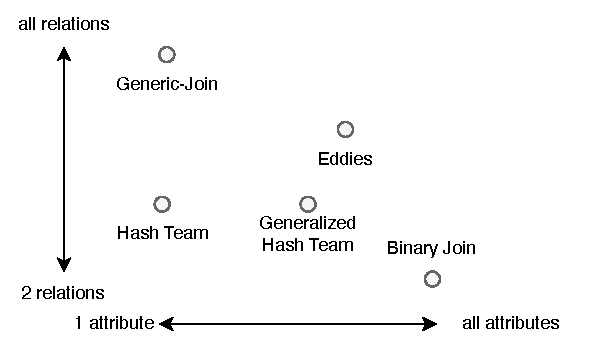
\includegraphics[width=0.55\linewidth]{free-join.pdf}
    \caption{Design space of join algorithms.}
    \label{fig:design-space}
\end{figure}

To explain these contributions we provide some context.
%
In this dissertation, we focus on algorithms based on hashing,
  and choose \GJ~\cite{DBLP:journals/sigmod/NgoRR13} as a representative of \WCOJ algorithms.
A crucial difference between \GJ and binary join lies 
  in the way they process each join operation. 
Binary join processes two relations at a time, 
  and joins on \emph{all attributes} 
  shared between these two relations. 
In contrast, \GJ processes one attribute at a time, 
  and joins \emph{all relations} that share that attribute.
This suggests a design space of join algorithms, 
  where each join operation may process any 
  number of attributes and relations.
Figure~\ref{fig:design-space} shows this design space
  which also covers classic multiway join algorithms 
  like Hash Team~\cite{DBLP:conf/vldb/GraefeBC98}, 
  Generalized Hash Team~\cite{DBLP:conf/vldb/KemperKW99}
  and Eddies~\cite{DBLP:conf/sigmod/HellersteinA00}.
Being able to join on any number of variables and relations
  frees us from the constraints of all existing algorithms 
  mentioned above. 
% } \yell{I suggest removing the boldface}

Our new framework, \FJ,
  covers the entire design space, 
  thereby generalizing and unifying existing algorithms.
The starting observation is that the execution of a {\em left-deep linear 
  binary join plan} (reviewed in Sec.~\ref{sec:background:fj}) is already very similar to \GJ.
While \GJ (also reviewed in Sec.~\ref{sec:background:fj}) is traditionally specified as a series of nested loops~\cite{DBLP:journals/sigmod/NgoRR13},
  the push-based model~\cite{DBLP:journals/pvldb/Neumann11,DBLP:journals/pvldb/KerstenLKNPB18} for executing a left-deep linear binary plan
  is also implemented, similarly, as nested loops.
% \rw{Should I add an example of the loop nest, or is that too much detail?}
% \ds{Not here, but please explain this point again in the technical
%   sections, and give an example there.}
The two algorithms also process each join operation similarly:
  each binary hash join iterates over tuples on one relation, 
  and for each tuple probes into the hash table of another relation;
  each loop level in \GJ iterates over the keys of a certain trie,
  and probes into several other tries for each key.
This inspired us to unify hash tables and hash tries into the same data structure, 
  and develop \FJ using iteration and probing as key operations.
This finer-grained view of join algorithms allows \FJ
  to generalize and unify existing algorithms,
  while precisely capturing each of them.

  \FJ takes as input an already optimized binary join plan, and
  converts it into a new kind of plan that we call a \FJ plan.  It
  then optimizes the \FJ plan, resulting in a plan that sits in
  between binary join and \GJ, combining the benefits of both.  On one
  hand \FJ fully exploits the design space in
  Figure~\ref{fig:design-space}.  On the other hand, by starting from
  an already optimized binary plan, \FJ takes advantage of existing
  cost-based optimizers; in our system we used binary plans produced by
  the optimizer of DuckDB~\cite{DBLP:conf/cidr/RaasveldtM20,DBLP:conf/vldb/Raasveldt22}.

Next, we address the main source of
  inefficiency in \GJ: the need to construct a trie on each relation
  in the query~\cite{DBLP:journals/pvldb/MhedhbiS19,DBLP:journals/pvldb/FreitagBSKN20}.  
In contrast,  a binary join plan needs to build a hash map only for each relation 
  on the right-hand side of a join,
  and simply iterates over the relation on the left.
As a result, a query optimizer commonly places the largest relation on the left
 to minimize the cost of hash building.
One simple optimization in \FJ is that we do not built a trie for
tables that are left children, mimicking the binary plans.
%
However, we go a step further, and introduce the {\em Column-Oriented
  Lazy Trie} (\COLT) data structure, which builds the inner subtries
  lazily, by creating each subtrie on demand.  
We note that this builds on an earlier idea
in~\cite{DBLP:journals/pvldb/FreitagBSKN20}.  As the name suggests,
\COLT adapts the lazy trie data structure
in~\cite{DBLP:journals/pvldb/FreitagBSKN20} to use a column-oriented
layout.  And unlike the original lazy trie which builds at least one
trie level per table, \COLT completely eliminates the cost of trie
building for left tables.


Finally, we describe a method for incorporating vectorized
  processing in \FJ, allowing it to collect multiple data values
  before entering the next iteration level.  
The standard \GJ processes one data value at a time, but, as is the
  case in traditional query engines, this leads to poor cache
  locality.  
Vectorized execution~\cite{DBLP:conf/icde/PadmanabhanAMJ01} was proposed for binary join
  to improve its locality by processing data values in batch.
By breaking down join operations into iterations and probes, 
  \FJ gives rise to a simple vectorized execution algorithm
  that breaks each iteration into chunks and groups together 
  batches of probes.
Our proposal is to our knowledge the first vectorized execution algorithm for \GJ.

We implemented \FJ as a standalone Rust library, and
compared it with two baselines:
  \begin{enumerate*}
    \item our own \GJ implementation in Rust, and
    \item the binary hash join implemented in
      DuckDB~\cite{DBLP:conf/cidr/RaasveldtM20,DBLP:conf/vldb/Raasveldt22},
      a state-of-the-art in-memory database.
    \end{enumerate*}
    %%%%%%%%%% No need for experimental details here, just some highlights
%%%   We conduct experiments on the popular Join Order
%%%   Benchmark~\cite{DBLP:journals/pvldb/LeisGMBK015} and the
%%%   LSQB~\cite{} benchmark.
  We found that, on acyclic queries, \FJ is up to \imdbmaxfjbj
  faster than binary join, and up to \imdbmaxfjgj faster than \GJ; on
  cyclic queries, \FJ is up to 15.45x faster than binary join, and up
  to 4.08x faster than \GJ.
  % \FJ also retains its advantage even when the optimizer chooses a poor plan.
%%%   We conduct additional experiments on
%%%   synthetic data for star and chain queries, as well as ablation
%%%   studies on the optimizations.  Finally, we compare \FJ and binary
%%%   hash join on their robustness against bad query plans.  Given a bad
%%%   query plan, \FJ runs up to \hjbad and \gjbad faster than binary join
%%%   and \GJ, respectively.

  While optimizers for binary plans have been developed and improved
  over decades~\cite{DBLP:conf/sigmod/SelingerACLP79}, little
  is known about optimizing \GJ.  A \GJ plan consists of a total order
  on its variables, and its run time depends on the choice of this
  order.  But since the theoretical analysis of \GJ guarantees worst
  case optimality for {\em any} variable order, it is a folklore
  belief that \GJ is more robust than binary join plans 
  when the optimizer makes a bad choice.
  To test the robustness of binary join, \GJ, and \FJ, 
  We also conducted experiments measuring their 
  performance when given a bad query plan.
  We found that \GJ is indeed the
  least sensitive, while \FJ, like binary joins, suffers more from the
  poor optimization choices of the optimizer, since both rely on a
  cost-based optimized plan.  However, \GJ starts from worse baseline
  than \FJ.  In other words, \FJ takes better advantage of a good
  plan, when available, than \GJ does.


  
In summary, we make the following contributions in this dissertation:
% \ds{Please reference the sections where these contributions are
%   described.  Currently the do NOT align with the contributions
%   mentioned earlier and discussed in the introduction.  This needs to
%   be fixed.}
% \rw{Fixed.}
\begin{enumerate}
  \item \FJ, a framework unifying existing join algorithms (Section~\ref{sec:free-join}).
  \item An algorithm to converting a binary plan into an
    optimized \FJ plan (Section~\ref{sec:bj-to-fj}).
  \item \COLT, a column-oriented lazy trie data structure (Section~\ref{sec:colt}).
  \item A vectorized execution algorithm for \FJ (Section~\ref{sec:vectorized-execution}).
  \item Experiments evaluating the algorithms and optimizations (Section~\ref{sec:eval}).
\end{enumerate}

\section{Background}\label{sec:background:fj}

This section defines basic concepts and reviews background on binary
join and \GJ.

\subsection{Basic Concepts}\label{sec:basic-concepts}

In previouse chapters we have used upper case variables for key values, 
 and reserved lower case variables for semiring values. 
As we do not deal with semirings in this chapter, 
 we will use lower case variables for key values to reduce clutter.
Recall from Section~\ref{sec:join} that a \emph{full conjunctive query} 
 has the following form:
%
\begin{align}
  Q(\bm x) \cd & R_1(\bm x_1), \ldots, R_m(\bm x_m). \label{eq:cq}
\end{align}
%
where each variable in a body atom $R_i({\bm x_i})$ also appears 
 in the head $R({\bm x})$.
We will assume that the query does not have {\em self-joins},
 meaning no two atoms share the same relation name.
This is without loss of generality: if two atoms have the same
relation name, then we simply rename one of them.  
Our system also supports selections, projections, and aggregation.  
We assume that the selections are pushed down to the base tables, thus the atom $R_i$
in~\eqref{eq:cq} may include a selection over a base table; in
particular, all variables in the atom $R_i(\bm x_i)$ are distinct.
Similarly, projections and aggregates are performed after the full
join, hence none of them is shown in~\eqref{eq:cq}.


\begin{ex} \label{ex:triangle} Consider the following SQL query:
\begin{lstlisting}[
    language=SQL,
    showspaces=false,
    basicstyle=\ttfamily\small,
    % numbers=left,
    % numberstyle=\tiny,
    commentstyle=\color{gray}
 ]
SELECT r.x, s.u, t.u
  FROM R as r, M as s, M as t -- schema: R(x,y), M(u,v,w)
 WHERE s.w > 30 AND t.v = t.w
   AND r.y = s.u AND s.v = t.u AND t.v = r.x
\end{lstlisting}
%
Then we denote by $S = \Pi_{uv}(\sigma_{w>30}(M))$ and $T =
\Pi_{uv}(\sigma_{v=w}(M))$, and write the query as:
$$Q_{\triangle}(x,y,z) \cd R(x, y), S(y,z), T(z, x).$$
%
We call this query the \emph{triangle query} over the relations $R$, $S$,
$T$.
\end{ex}

It is often convenient to view the conjunctive query~\eqref{eq:cq} as
a hypergraph.  The \emph{query hypergraph} of $Q$ consists of vertices
$\mathcal{V}$ and edges $\mathcal{E}$, where the set of nodes
$\mathcal{V}$ is the set of variables occurring in $Q$, and the set of
hyperedges $\mathcal{E}$ is the set of atoms in $Q$.  The hyperedge
associated to the atom $R(\bm x_i)$ is defined as the set consisting
of the nodes associated to the variables $\bm x_i$.  As standard, we
say that the query $Q$ is {\em acyclic} if its associated hypergraph
is $\alpha$-acyclic~\cite{DBLP:journals/jacm/Fagin83}


\subsection{Binary Join}\label{sec:binary-join}

The standard approach to computing a conjunctive query~\eqref{eq:cq} is
to compute one binary join at a time.  A {\em binary plan} is a binary
tree, where each internal node is a join operator $\Join$, and each
leaf node is one of the base tables (atoms) $R_i(\bm x_i)$ in the
query~\eqref{eq:cq}.  The plan is a \emph{left-deep linear plan}, or
simply left-deep plan, if the right child of every join is a leaf
node.  If the plan is not left-deep, then we call it \emph{bushy}.
For example, $(R \Join S) \Join (T \Join U)$ is a bushy plan, while
$((R \Join S) \Join T) \Join U$ is a left-deep plan.  We do not treat
specially right-deep or zig-zag plans, but simply consider them to be
bushy.

In this dissertation we consider only hash-joins, which are the most
common types of joins in database systems. 
The standard way to execute a bushy plan is to
decompose it into a series of left-deep linear plans.  Every join node
that is a right child becomes the root of a new subplan, which is
first evaluated, and its result materialized, before the parent join
can proceed.  As a consequence, every binary plan, bushy or not,
becomes a collection of left-deep plans. 
In our system we decompose bushy
plans exactly this way, and we will focus on left-deep linear
plans in the rest of this chapter.  For example, the bushy plan
$(R \Join S) \Join (T \Join U)$ is converted into two plans:
$P_1 = T \Join U$ and $P_2 = (R \Join S) \Join P_1$; both are
left-deep plans.

To reduce clutter, we represent a left-deep plan
$(\cdots ((R_1 \Join R_2) \Join R_3) \cdots \Join R_{m-1}) \Join R_m$
as $[R_1, R_2, \ldots, R_m]$.  Evaluation of a left-deep plan is done
using pipelining.  The engine iterates over each tuple in the
left-most base table $R_1$; each tuple is probed in $R_2$; each of the
matching tuple is further probed in $R_3$, etc.


\begin{figure}
  \begin{subfigure}[b]{0.5\linewidth}
\centering
\begin{tabular}{c}
\begin{lstlisting}
for (x, y) in R:
  s = S[y]?
  for (y, z) in s:
    t = T[x,z]?
    for (x, z) in t:
      output(x, y, z)
\end{lstlisting}
\end{tabular}
\caption{Binary join.}
\label{fig:background:binary-join}
  \end{subfigure}
% \hspace{2cm}
  \begin{subfigure}[b]{0.45\linewidth}
\centering
\begin{tabular}{c}
\begin{lstlisting}
for a in R.x $\cap$ T.x:
  r = R[a]; t = T[a]
  for b in r.y $\cap$ S.y:
    s = S[b]
    for c in s.z $\cap$ t.z:
      output(a, b, c)
\end{lstlisting}
\end{tabular}
    \caption{\GJ.}
    \label{fig:background:gj}
  \end{subfigure}
%  \Description[TODO]{TODO}
  \caption{Execution of binary join and \GJ for $Q_\triangle$.  The
    notation \lstinline|S[y]?| performs a lookup on $S$ with the key
    $y$, and continues to the enclosing loop if the lookup fails.
    Binary join iterates over {\em tuples}, \GJ iterates over {\em
      values}.}
\end{figure}

\begin{ex}
  A possible left-deep linear plan for $Q_\triangle$ is $[R, S, T]$,
  which represents $(R(x,y) \Join S(y,z)) \Join T(z,x)$.  To execute
  this plan, we first build a hash table for $S$ keyed on $y$, where
  each $Y$ maps to a vector of $(y,z)$ tuples, 
  % \yell{Remy: this is not
  %   correct.  The hash table contains tuples.  Think of a table that
  %   has 30 attributes $S(x_1,\ldots, x_{30})$.  If you join on
  %   $x_{12}$, you don't create a new tuple with 29 attributes, but
  %   store the whole tuple in the hash table.  Some systems actually
  %   store a pointer to the real tuple in the buffer pool.}
  and a hash table for $T$ keyed on $x$ and $z$, each mapped to a
  vector of $(x,z)$ tuples\footnote{When the relations are bags, then
    the hash table may contain duplicate tuples, or store separately
    the multiplicity.  We also note that the question what exactly to
    store in the hash table (e.g. copies of the tuples, or pointers to
    the tuple in the buffer pool) has been studied for a long time,
    see~\cite{DBLP:journals/csur/Graefe93}.}.  Then the execution
  proceeds as shown in Figure~\ref{fig:background:binary-join}.  For each
  tuple $(x, y)$ in $R$, we first probe into the hash table for $S$
  using $y$ to get a vector of $(y, z)$ tuples.  We then loop over
  each $(y, z)$ and probe into the hash table for $T$ using $x$ and
  $z$.  Each successful probe will return a vector of $(x, z)$ tuples,
  and we output the tuple $(x, y, z)$ for each $(x, z)$.
\end{ex}

\subsection{\GJ}\label{sec:background:gj}

\GJ was introduced in~\cite{DBLP:journals/sigmod/NgoRR13} and is the
simplest worst-case optimal join algorithm.  It is based on the
earlier Leapfrog Triejoin algorithm~\cite{DBLP:conf/icdt/Veldhuizen14}.
%
\GJ computes the query $Q$ in~\eqref{eq:cq} through a series of nested
loops, where each loop iterates over a variable (not a tuple).
Concretely, \GJ chooses arbitrarily a variable $x$, computes the
intersection of all $x$-columns of all relations containing $x$, and
for each value $a$ in this intersection it computes the residual query
$Q[a/x]$, where every relation $R$ that contains $x$ is replaced with
$\sigma_{x=a}(R)$.  In pseudocode:
%
\begin{lstlisting}
GJ: for a in $\bigcap \setof{\Pi_x(R_i)}{R_i \mbox{ contains } x}$
      compute Q[a/x]  \\ run GJ on Q with one fewer variable
\end{lstlisting}
%
If the query $Q$ has $k$ variables, then there are $k$ nested loops in
\GJ.  In the inner most loop, \GJ outputs the tuple of constants, one
from each iteration.\footnote{For bag semantics, it multiplies their
  multiplicities.}  We notice that a plan for \GJ consists of a total
order of the variables of the query, which we denote as
$[x_1, x_2, \ldots, x_k]$.  Assuming that the intersection above is
done optimally (see below), the algorithm is provably
worst-case-optimal, for any choice of the variable order.

\begin{ex}
  Fig.~\ref{fig:background:gj} illustrates the pseudocode for \GJ on the
  query $Q_\triangle$, using the variable order $[x,y,z]$.  We denoted
  $\Pi_x(R)$ by $R.x$, and denoted (with some abuse) $\sigma_{x=a}(R)$
  by $R[a]$.
\end{ex}


While binary joins use hash tables, an implementation of \GJ uses a
\emph{hash trie}, one for each relation in the query.  The hash-trie
is a tree, whose depth is equal to one plus the number of attributes
of the relation, and where each node is either an empty leaf
node,\footnote{For bag semantics, we store in the leaf the
  multiplicity of the tuple.} or a hash map mapping each atomic value
to another node.  We will call the \emph{level} of a node to be the
distance from the root, i.e. the root has level 0, its children level
1, etc.  The hash-trie completely represents the relation: every
root-to-leaf path corresponds precisely to one tuple in the relation.
\GJ uses the hash-trie as follows.  In order to compute
$\sigma_{x=a}(R)$, it simply probes the current hash table for the
value $x=a$, and returns the corresponding child.  To compute an
intersection $\Pi_x(R_1) \cap \Pi_x(R_2) \cap \cdots$, it selects the
trie with the fewest keys, say $R_1$, then iterates over every value
$a$ in the keys for $R_1$ and probes it in each of the hash-maps for
$R_2, R_3, \ldots$; this is a provably optimal algorithm for the
intersection.

\begin{ex}
  Consider the query $Q_\triangle$ and the \GJ plan $[x, y, z]$.  We
  first build a hash trie each for $R$, $S$, and $T$.  Each trie has
  three levels including the leaf.  Level 0 of $R$ is keyed on $x$,
  level 1 is keyed on $y$, level 2 contains empty leaf nodes, and
  similarly for $S$ and $T$.  Consider again the pseudocode in
  Figure~\ref{fig:background:gj}.  The first loop intersects level 0
  of the $R$-trie and the $T$-trie.  For each value $a$ in the
  intersection, we retrieve the corresponding children $R[a]$ and
  $T[a]$ respectively; these are at level 1.  The second loop
  intersects the hash map $R[a]$ (at level 1) with the level 0
  hash-map of $S$.  For each value $b$ in the intersection it
  retrieves the corresponding children (levels 2 and 1 respectively),
  and, finally, the innermost loop intersects the $S$- and $T$-hash
  maps (both at level 2), and outputs $(a,b,c)$ for each $c$ in the
  intersection.  So far we have assumed set semantics; if the
  relations have bag semantics, then we simply multiply the tuple
  multiplicities on the leaves (level 3).
\end{ex}

%%% The original \GJ algorithm was specified for set semantics,
%%% however~\cite{DBLP:journals/pvldb/FreitagBSKN20} showed the algorithm
%%% can be easily extended to bag semantics.  We therefore ignore the
%%% difference between the two semantics for the rest of this dissertation.

\subsection{Binary Join v.s. \GJ}
Binary join and \GJ each have their own advantages and disadvantages.
\GJ became popular because of its asymptotic performance guarantee:
\cite{DBLP:journals/sigmod/NgoRR13} proved the algorithm is
\emph{worst-case optimal} for \emph{any variable order}, in the sense
that its run time is bounded by the largest possible size of its
output, called AGM bound~\cite{DBLP:journals/siamcomp/AtseriasGM13}.
For example, \GJ executes $Q_\triangle$ in time
$\sqrt{|R|\cdot |S| \cdot |T|}$, which is $n^{3/2}$ when all relations
have size $n$; in contrast, a binary join plan can take $\Omega(n^2)$.
We note, however, that this formula does not include the preprocessing
time needed to construct the tries.  For example, if $T$ is
significantly larger than $R, S$, then the run time of \GJ is
$\ll |T|$, yet during preprocessing \GJ needs to read the entire
relation $T$.  On the other hand, binary join has been a staple of
database systems for decades.  The hash table data structure is
simpler than hash tries and is cheaper to build.  Techniques like
vectorized execution and column-oriented layout have also made binary
join practically efficient, but these optimizations have not been
adapted for \GJ.  Binary join plans are known to be very sensitive to
the choice of the optimizer: poor plans perform catastrophically
bad~\cite{DBLP:journals/pvldb/LeisGMBK015}.  In contrast, although the
runtime performance of \GJ does depend on the variable order, some
researchers believe that \GJ is less sensitive to poor variable
orders, in part because it is worst-case optimal.

\section{\FJ}\label{sec:free-join}

In this section we introduce the \FJ framework.
We start by presenting the Generalized Hash Trie (\GHT) which
 is the data structure used in \FJ (Section~\ref{sec:ght}).
Next we introduce the \FJ plan that specifies 
  how to execute a query with \FJ (Section~\ref{sec:fj-plan}).
Finally, we describe the \FJ algorithm, 
  which takes as input a collection of \GHTs 
  and a \FJ plan,
  and computes the query according to the plan (Section~\ref{sec:free-join-algorithm}).
  
We will show how each of the above components generalizes 
  and unifies the corresponding components in binary join 
  and \GJ: 
  the \GHT generalizes hash tables and hash tries,
  the \FJ plan generalizes binary plans and \GJ plans, and
  the \FJ algorithm generalizes binary join and \GJ.

\begin{figure}
\begin{subfigure}[b]{0.49\linewidth}
\begin{align*}
  Q_{\clubsuit}(x,a,b,c) \cd R(x,a),S(x,b),T(x,c)
\end{align*}
\begin{alignat*}{4}
  R & = \set{(x_0, a_0)} && \cup \{(x_1, a_i^l), (x_2, a_i^r &&) \mid i \in [1 \ldots n] \} \\
  S & = \set{(x_0, b_0)} && \cup \{(x_2, b_i^l), (x_3, b_i^r &&) \mid i \in [1 \ldots n] \} \\
  T & = \set{(x_0, c_0)} && \cup \{(x_3, c_i^l), (x_1, c_i^r &&) \mid i \in [1 \ldots n] \} 
  % R & = \set{(x_0, a_0)} \cup \bigcup_{i \in [1 \ldots n]} \set{(x_1, a_i^l), (x_2, a_i^r)} \\
  % S & = \set{(x_0, b_0)} \cup \bigcup_{i \in [1 \ldots n]} \set{(x_2, b_i^l), (x_3, b_i^r)} \\
  % T & = \set{(x_0, c_0)} \cup \bigcup_{i \in [1 \ldots n]} \set{(x_3, c_i^l), (x_1, c_i^r)} 
\end{alignat*}
\caption{$Q_\clubsuit$ and inputs.}
\label{fig:clover-query}
\end{subfigure}
\begin{subfigure}[b]{0.5\linewidth}
  \centering
  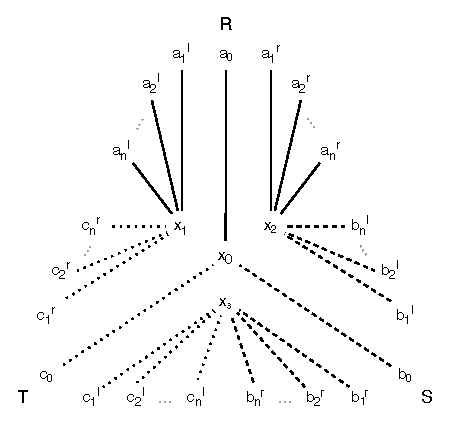
\includegraphics[width=0.8\linewidth]{sand-dollar.pdf}
  \caption{Visualization of the input relations.}
  \label{fig:clover-vis}
\end{subfigure}
\caption{(\ref{fig:clover-query}) the clover query $Q_\clubsuit$, and an input instance.
(\ref{fig:clover-vis}) visualization of the instance in
    Fig.~\ref{fig:clover-query}. The solid (top) edges form the relation
    \texttt{R}, the dashed (right) edges form the relation \texttt{S},
    and the dotted (left) edges form the relation \texttt{T}.  The
    relations join on the attribute in the center.  The only output
    tuple consists of the three edges in the center. }
\end{figure}

Throughout this section we will make use of the {\em clover query}
$Q_\clubsuit$ in Figure~\ref{fig:clover-query}.
Figure~\ref{fig:clover-vis} visualizes the input relations for this query.
Note that $Q_\clubsuit$ is
\emph{acyclic}.

\subsection{The Generalized Hash Trie}\label{sec:ght}

\begin{figure}
\begin{lstlisting}
interface GHT {
  # fields
  relation: String, vars: Vec<String>  
  # constructor
  fn new(name: String, schema: Vec<Vec<String>>) -> Self
  # methods
  fn iter() -> Iterator<Tuple>
  fn get(key: Tuple) -> Option<GHT> }
\end{lstlisting}
\caption{The \GHT interface.}
\label{fig:ght}
\end{figure}

To unify binary join and \GJ, 
  we first need to unify the data structures they work over.
We propose the Generalized Hash Trie 
  which generalizes both the hash table used in binary join 
  and the hash trie used in \GJ.

\begin{defn}[Generalized Hash Trie (\GHT)]
  A \GHT is a tree where each leaf is a vector of tuples, and
  each internal node is a hash map whose keys are tuples, and each key
  maps to a child node.
\end{defn}

We will reuse the terminology defined for tries, including
\emph{level}, \emph{node}, and \emph{leaf}, etc., for \GHTs.  We will
also use the terms \GHT and \emph{trie} interchangeably when the
context is clear.  The {\em schema} of a \GHT is the list
$[\bm y_0,\bm y_1, \ldots, \bm y_\ell]$ where $\bm y_k$ are the
attribute names of the key at level $k$. 

The hash trie used in \GJ is a \GHT where each key is a tuple of size one,
  and the last level stores empty vectors, each of which represents a leaf.
The hash table used in binary join is very similar to a \GHT with only two levels,
  where level 0 stores the keys and level 1 stores
  vectors of tuples.
A small difference is that, in the \GHT, the concatenation of 
  a tuple from level 0 with a tuple from level 1 forms a tuple in the relation, 
  whereas each whole tuple is stored directly in a hash table.
We will show in Section~\ref{sec:colt} how the \COLT data structure
  more faithfully captures the structure of a hash table.
Figure~\ref{fig:ght-examples} shows two examples of \GHTs.

We use \GHTs to represent relations,
  and attach metadata as well as access methods 
  to each \GHT, to be used by the \FJ algorithm.
The \GHT interface is shown in Figure~\ref{fig:ght}.
The \lstinline|relation| field stores the relation name.
A sub-trie inherits its name from its parent.
The \lstinline|vars| field stores parts of the relation's schema:
  if the trie is a vector of tuples, 
  \lstinline|vars| is the schema of each tuple;
  if the trie is a map, 
  \lstinline|vars| is the schema of each key.
The constructor method \lstinline|new| creates a new \GHT from the named relation, 
  where an $n$-th level trie has variables
  matching the $n$-th element of the \lstinline|schema| argument,
  and the values along each path from the root to a leaf of the \GHT 
  form a tuple in the relation.

\begin{ex}
  Both \GHTs in Figure~\ref{fig:ght-examples} represent relation $S$ from the
  clover query $Q_\clubsuit$ in Figure~\ref{fig:clover-query}.  The
  \GHT on the left (a hash trie) was created by calling the
  constructor method \lstinline|new| with the schema
  \lstinline|[[x],[b],[]]|, so the top-level trie has the schema
  \lstinline|[x]|, each second-level trie has the schema
  \lstinline|[b]|, and each third-level trie (a leaf) has the empty
  schema \lstinline|[]|.  The \GHT on the right (a hash table) was
  created by calling \lstinline|new| with the schema
  \lstinline|[[x],[b]]|.  It has only two levels, with schema
  \lstinline|[x]| and \lstinline|[b]|, respectively.  Note that each
  $b$ value in the hash trie is hashed and stored as a key, while the
  $b$ values in the hash table are simply stored in vectors.
\end{ex}

The methods \lstinline|iter| and \lstinline|get| 
  provide access to values stored in the trie.
If the trie is a map, 
  \lstinline|get(key)| returns the sub-trie mapped to \lstinline|key|,
  if any.
Calling \texttt{get} on a vector returns \lstinline|None|.
If the trie is a vector, 
  \lstinline|iter()|
  returns an iterator over the tuples in the vector;
  calling \texttt{iter} on a map 
  returns an iterator over the keys.

\begin{figure}
  \centering
  \begin{subfigure}[c]{0.3\linewidth}
  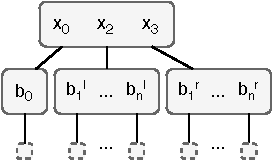
\includegraphics[width=\textwidth]{trie}
  \end{subfigure}\hspace{1.5cm}%
  \begin{subfigure}[c]{0.3\linewidth}
  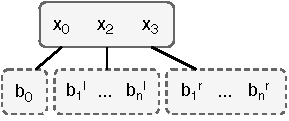
\includegraphics[width=\textwidth]{map}
  \end{subfigure} 
  \caption{
    Two \GHTs. The one on the left is also a hash trie, 
      and the one on the right is similar to a hash table.
    Each box with solid border stores hash keys, 
    and each box with dashed border is a vector of tuples.
    An empty box is an empty vector, representing a leaf.
  }
  \label{fig:ght-examples}
\end{figure}

\begin{ex}
  On the second \GHT in Figure~\ref{fig:ght-examples},
    calling \texttt{iter} returns an 
    iterator over the values $[x_0, x_2, x_3]$.
    Calling \texttt{get} with the key $x_2$ 
    returns the sub-trie which is the vector $[b_1^l, \ldots, b_n^l]$.
  Calling \texttt{iter} on this sub-trie
    returns an iterator over $[b_1^l, \ldots, b_n^l]$.
\end{ex}


\subsection{The \FJ plan}\label{sec:fj-plan}

% \ds{The section tile doesn't seem right.  What about ``The \FJ plan''}

A \FJ plan specifies how the \FJ algorithm should be executed.
It generalizes and unifies binary join plans and \GJ plans. 
Recall that a left-deep linear plan for binary join
  is a sequence of relations;
  it need not specify the join attributes, 
  since all shared attributes are joined.
In contrast, a \GJ plan is a sequence of variables;
  it need not specify the relations, 
  since all relations on each variable are joined.
A \FJ plan may join on any number of variables and relations at each step,
  and therefore needs to specify both explicitly.

  To help define the \FJ plan, we introduce two new concepts, called
  \emph{subatom} and \emph{partitioning}.  Fix the query $Q$ in
  Eq.~\eqref{eq:cq}:

\begin{defn}
  A \emph{subatom} of an atom $R_i(\bm x_i)$ is an expression
  $R_i(\bm y)$ where $\bm y$ is a subset of the variables $\bm x_i$.
  A \emph{partitioning} of the atom $R_i(\bm x_i)$ is a set of
  subatoms $R_i(\bm y_1), R_i(\bm y_2), \ldots$ such that
  $\bm y_1, \bm y_2, \ldots$ are a partition of $\bm x_i$.
\end{defn}

We now define the \FJ plan using these concepts.

\begin{defn}[\FJ Plan]
  Fix a conjunctive query $Q$.  A \FJ \emph{plan} is a list
  $[\phi_1, \ldots, \phi_m]$, where each $\phi_k$ is a list of
  subatoms of $Q$, called a {\em node}.  The nodes are required to
  {\em partition the query}, in the sense that, for every atom
  $R_i(\bm x_i)$ in the query, the set of all its subatoms occurring
  in all nodes must form a partitioning of $R_i(\bm x_i)$.  We denote
  by $vs(\phi_k)$ the set of variables in all subatoms of $\phi_k$.
  The variables \emph{available to} $\phi_k$ are all the variables of the
  preceding nodes:
%
$$avs(\phi_k) = \bigcup_{j < k} vs(\phi_j)$$
%
\end{defn}

%%% Since the partitioning of each atom into subatoms can be inferred 
%%%   from the sequence of nodes, we will omit the partitioning 
%%%   when specifying a \FJ plan.

We will define shortly a {\em valid plan}, but first we show an example.

%%% While a \GJ plan consists of total order of the variables, a \FJ plan
%%% defines only a partial order, if we set
%%% $vs(\Phi_i) < vs(\Phi_2) < \cdots$.


\begin{ex}\label{ex:fj-plan}
  The following is an \FJ plan for $Q_\clubsuit$:
\begin{align}
&  [[R(x, a), S(x)], [S(b), T(x)], [T(c)]]\label{eq:bj-plan}
\end{align}
%
To execute the first node we iterate over each tuple $(x, a)$ in $R$
and use $x$ to probe into $S$; for each successful probe we execute
the second node: we iterate over each $b$ in $S[x]$, then use
$x$ to probe into $T$; finally the third node iterates over $c$ in
$T[x]$.  The reader may notice that this corresponds precisely to the
left-deep plan $(R(x,a) \Join S(x,b))\Join T(x,c)$.
%
Another \FJ plan for $Q_\clubsuit$ is: 
%
\begin{align}
  [[R(x), S(x), T(x)], [R(a)], [S(b)], [T(c)]]\label{eq:gj-plan}
\end{align}
%
This plan corresponds to the \GJ plan $[x,a,b,c]$.  Intuitively, here
we start by intersecting $R.x \cap S.x \cap T.x$, then, for each $x$
in the intersection, we retrieve the values of $a$, $b$, and $c$ from
$R$, $S$, and $T$, and output their Cartesian product.
\end{ex}

% \begin{figure}
%   \begin{subfigure}[t]{0.4\linewidth}
%     \centering
%     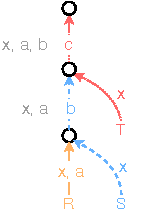
\includegraphics[height=35mm]{fj.pdf}
%     \caption{Plan in Eq.~\eqref{eq:bj-plan} (binary)}
%     \Description[TODO]{TODO}
%     \label{fig:bj-plan}
%   \end{subfigure}
%   \begin{subfigure}[t]{0.5\linewidth}
%     \centering
%     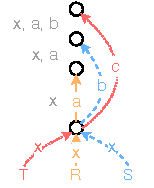
\includegraphics[height=32mm]{gj.pdf}
%     \caption{Plan in Eq.~\eqref{eq:gj-plan} (\GJ)}
%     \label{fig:gj-plan}
%   \end{subfigure}
%   \caption{Visualization of \FJ plans using notations from tensor
%     algebra~\cite{DBLP:journals/pacmpl/KjolstadKCLA17}.  Each circle
%     is a join node.  Arrows pointing to a node indicate the subatoms
%     in that node.  The same color and line style signify the same
%     relation. Grey text shows available variables.}
%   \label{fig:fj-plans}
% \end{figure}

% Readers familiar with tensor algebras may view \FJ as an
% \emph{iteration graph}~\cite{DBLP:journals/pacmpl/KjolstadKCLA17}, as
% shown in Figure~\ref{fig:fj-plans}.  We can ``read off'' the binary
% join plan $[R, S, T]$ from Figure~\ref{fig:bj-plan} by ignoring the
% variables.  Similarly, if we follow the variables in
% Figure~\ref{fig:gj-plan} bottom-up and ignore duplicates, we obtain the \GJ
% plan $[x, a, b, c]$.

Not all \FJ plans are valid, and only valid plans can be executed.  We
execute each \FJ node by iterating over one relation in that node, and
probe into the others.  Therefore, the values used in each probe must
be available, either from the same node or a previous one.

\begin{defn}
  A \FJ plan is \emph{valid} if for every node $\phi_k$ the following
  two properties hold.  (a) No two subatoms share the same relation,
  and (b) there is a subatom containing all variables in
  $vs(\phi_k) - avs(\phi_k)$.  We call such an subatom a \emph{cover}
  for $\phi_k$, and write $cover(\phi_k)$ for the set of covers.
\end{defn}

We will assume only valid plans in the rest of the paper.  To simplify
the presentation, in this section we assume that each node $\Phi_k$,
has {\em one} subatom designated as cover, and will always list it as
the first subatom in $\Phi_k$.  We will revisit this assumption in
Sec.~\ref{sec:optimization}, and allow for multiple covers.

%%% By this definition, every node must contain at least one subatom.  In
%%% addition, since we rename relations in a self-join as described in
%%% Section~\ref{sec:background}, a variable cannot appear in more than
%%% one subatom with the same relation name, and the same variable cannot
%%% appear more than once in the same subatom.

\begin{ex}
  Both plans in Example~\ref{ex:fj-plan} are valid.  The covers for
  the 3 nodes for Eq.~\eqref{eq:bj-plan} are $R(x, a)$, $S(b)$, and
  $T(c)$, respectively. For the plan in Eq.~\eqref{eq:gj-plan}, the
  covers for the 4 nodes are $R(x), R(a), S(b), T(c)$; for the first
  node we could have also chosen $S(x)$ or $T(x)$ as cover.
\end{ex}
 
% \ds{A few issues in the paragraph above and earlier.  You need to
%   define an atom, since this seems to be nonstandard: I assume you
%   mean that an atom consists of a relation name and a subset of the
%   variables.  The statement ``we do not allow self-joins'' raises
%   eyebrows; I don't think you mean that, please clarify.  The last
%   restriction (no atom contains the same variable twice) is OK, but
%   should be stated and explained in Sec.~\ref{sec:background}.}
% \rw{Will clarify in Backgroud.
%  For self-joins, we do allow them, but we rename the relation names to be different,
%  so that it looks like a join between different relations.
%  I'll also clarify this in Backgroud.  }
% \rw{Add because we rename them.}
% \rw{Use partial atom instead of an atom.}

% \ds{Before the next example add a brief explanation why the plans in
%   Ex.~\ref{ex:fj-plan} are valid.}
\begin{ex}
  An example of an \emph{invalid} plan for the clover query has one
  single node containing all relations and variables:
%
  $$[[R(x, a), S(x, b), T(x, c)]]$$
%
  Intuitively, we cannot execute it: if we iterate over, say $R$, then
  we bind two variables $x$ and $a$, but to lookup $S$ we
  need the key $(x,b)$.
\end{ex}

% \rw{We partition each atom to subatoms, 
% and define a plan for the query.
% }
% \begin{defn}
%   Given a \FJ plan $[\phi_1, \ldots, \phi_n]$, where 
% $\phi_i = \set{R_1(\overline{x_{i,1}}), \ldots, R_m(\overline{x_{i,m}})}$,
% \FJ computes the query:
% $$Q(*) \cd R_1(\overline{x_{1,1}}, \ldots, \overline{x_{n,1}}), \ldots, R_m(\overline{x_{1,m}}, \ldots, \overline{x_{n,m}}).$$
% That is, for each relation, we concatenate all its variables in the plan in order to form the query. 
% \end{defn}

% \begin{ex}
%   Both plans in Eq.~\eqref{eq:bj-plan} and Eq.~\eqref{eq:gj-plan} 
%   compute the clover query $Q(x,a,b,c) \cd R(x,a), S(x,b), T(x,c).$
% \end{ex}

% \ds{Add a definition saying ``Given a plan $P$, the query computed by
%   $P$ is $\ldots$'' Then illustrate this defintion with
%   Example~\ref{ex:fj-plan} and the example below.}

% \begin{ex}
%   The plan $[\phi=\set{R(), S(), T()}]$ is valid and computes the three-way 
%   Cartesian product of the relations (it does not compute the clover query).
%   The plan is vacuously valid because $vs(\phi) = \emptyset$.
%   Both plans in Eq.~\eqref{eq:bj-plan} and Eq.~\eqref{eq:gj-plan} are also valid.
% \end{ex}

% \ds{Equation numbers should be referred to using $\backslash$eqref
%   instead of $\backslash$ref.  I changed them in this file.}

\subsection{Execution of the \FJ Plan}\label{sec:free-join-algorithm}

% \ds{Suggestion: I would call this section ``Execution of the \FJ
%   Plan'' to better connect it to the previous section.}

The execution of a \FJ plan has two phases: the build phase and the
join phase.  The build phase constructs the \GHTs for the relations in
the query, by calling the constructor method \lstinline|new| on each
relation with the appropriate schema.  The join phase works over the
\GHTs to compute the join of the relations.

% fn ght_schema(relation, plan):
%   schema = []
%   for node in plan:
%     for atom in node:
%       if atom.relation == relation:
%         schema.append(atom.variables)
%   return schema 

\begin{figure}
  \begin{lstlisting}[
    commentstyle=\color{gray},
    escapeinside={(*}{*)},
    ]
fn join(all_tries, plan, tuple):
  if plan == []:
    output(tuple) (* \label{lst:output} *)
  else:
    tries = [ t $\in$ all_tries | t.relation $\in$ plan[0] ] (* \label{lst:select} *)
    # iterate over the cover
    @outer for t in tries[0].iter(): (* \label{lst:outer} *)
      subtries = [ iter_r.get(t) ] (* \label{lst:inner} *)
      tup = tuple + t
      # probe into other tries
      for trie in tries[1..]:     
        key = tup[trie.vars] (* \label{lst:key} *)
        subtrie = trie.get(key)
        if subtrie == None: continue @outer
        subtries.push(subtrie) (* \label{lst:inner-end} *)
      new_tries = all_tries[tries $\mapsto$ subtries] (* \label{lst:tuple} *)
      join(new_tries, plan[1:], tup) (* \label{lst:join} *)
\end{lstlisting}
  \caption{The \FJ algorithm.}
  \label{fig:fj-algo}
\end{figure}

\subsubsection*{Build Phase}
The build phase constructs a \GHT for each relation (atom)
$R_i(\bm x_i)$, as follows.  If the plan partitions the atom into the
subatoms $R_i(\bm y_0), R_i(\bm y_1), \ldots, R_i(\bm y_{\ell-1})$,
then the schema of its \GHT is the list
$[\bm y_0, \bm y_1, \ldots, \bm y_{\ell-1}, []]$.  Recall that the
last level of a \GHT is a vector instead of a hash map. As an
optimization, if the last subatom $R_i(\bm y_{\ell-1})$ is the cover
of its node, then we drop the last $[]$ from the schema, in other
words, we construct a vector for the $\bm y_{\ell-1}$.  After
computing the schema for each relation, we call the constructor method
\lstinline|new| on each relation and its computed schema to build the
\GHTs.

\begin{ex}
  Consider the plan in Eq.~\eqref{eq:bj-plan} for the clover query
  $Q_\clubsuit$.  The \GHT schemas for $R$, $S$, and $T$ are
  $[[x, a]]$, $[[x], [b]]$, and $[[x], [c]]$ respectively.  Thus, $R$
  is a flat vector of tuples, and each of $S$ and $T$ is a hash map of
  vectors of values.  Consider now the triangle query $Q_{\triangle}$
  and the plan $[[R(x,y),S(y),T(x)],[S(z),T(z)]]$.  The \GHT
  schemas for $R, S, T$ are $[[x,y]]$, $[[y],[z]]$, and $[[x],[z],[]]$:
  in other words $R$ is stored as a vector, $S$ is a hash-map of
  vectors, and $T$ is a hash-map of hash-maps of vectors.
\end{ex}

\subsubsection*{Join Phase}
The pseudo-code for the \FJ algorithm is shown in Figure~\ref{fig:fj-algo}.
The \lstinline|join| method takes as input the \GHTs, the \FJ plan, 
  and the current tuple initialized to be empty.
If the plan is empty, we output the tuple (line~\ref{lst:output}).
Otherwise, we work on the first node in the plan
  and intersect relevant tries (line~\ref{lst:select}).
We iterate over tuples in the covering relation, 
  which is the first trie in the node (line~\ref{lst:outer}).
%
% First we pick the trie to iterate over (line~\ref{lst:iter}).
% If any trie is a vector, we iterate over it.
% % \dan{I think it's clearer if you always iterate over the first
% %   subatom, which is the cover of the node.  We just need to make sure
% %   that this subatom is a vector, when that's possible.}
% % For now, we assume for each join node, at most one trie is a vector.
% % %
% % \yell{At this point there is nothing left to assume.  The \GHT is well
% %   defined, and only its last level is a vector, and the \GHT schema
% %   for a plan is well defined.  Everything is well defined.}
% % %
% We will relax this assumption in Section~\ref{sec:colt}.
% If all tries are hash maps, we iterate over the one with the fewest keys.
% After picking the trie to iterate over, 
%   we sort the other tries by some estimated cost to probe into them (line~\ref{lst:probe}).
% For example, we can probe into the smaller trie first, 
%   since it is likely to be selective, and may fit into the cache.
%
% In the outer for loop (line~\ref{lst:outer})
%   we iterate over each tuple \lstinline|t| in the trie we have picked.
Then, we use values from \lstinline|t| 
  and the \lstinline|tuple| argument
  as keys to probe into the other tries 
  (line~\ref{lst:inner}-\ref{lst:inner-end}).
To construct a key for a certain trie, 
  we find the values mapped from the trie's schema variables
  in \lstinline|t| and \lstinline|tuple| (line~\ref{lst:key}).
If any probe fails, we continue to the next tuple in the outer loop.
If all probes succeed, we replace the original tries with the 
  subtries returned by the probes,
  and recursively call \lstinline|join| 
  on the new tries and the rest of the plan (line~\ref{lst:tuple}-\ref{lst:join}).

The recursive definition may obscure the essence of the \FJ algorithm,
  so we provide some examples where we unroll the recursion.
We introduce some convenient syntax to simplify the presentation.
We write \lstinline|for (x,y,...) in T:| 
  to introduce a for-loop iterating over \lstinline|T|, 
  binding the values of each tuple in \lstinline|T.iter()| 
  to the variables \lstinline|x,y,...|.
We write \lstinline|r = R[t]?| to bind the result of 
  \lstinline|R.get(t)| to \lstinline|r|;
  if the lookup fails, we continue to the next iteration of the 
  enclosing loop.
In other words, \texttt{r = R[t]?} is equivalent to:
%
\begin{lstlisting}
r = R.get(t); if r.is_none(): continue
\end{lstlisting}

\begin{figure*}
  \begin{subfigure}[b]{0.3\linewidth}
\begin{lstlisting}[escapeinside={(*}{*)}]
R = GHT("R",[["x","a"]])
S = GHT("S",[["x"],["b"]])
T = GHT("T",[["x"],["c"]])
for (x, a) in R:
  s = S[x]?
  for b in s:
   (* \underline{t = T[x]?} *)
    for c in t:
      output(x, a, b, c)
\end{lstlisting}
    \caption{Binary \FJ.}
    \label{fig:bj-loop}
  \end{subfigure}
\hspace{1.5em}
  \begin{subfigure}[b]{0.3\linewidth}
    \centering
\begin{lstlisting}[
    escapeinside={(*}{*)}
]
# same as the left
# ...
# ...
for (x, a) in R:
  s = S[x]?
 (* \underline{t = T[x]?} *)
  for b in s:
    for c in t:
      output(x, a, b, c)
\end{lstlisting}
    \caption{Factorized \FJ.}
    \label{fig:factorized-loop}
  \end{subfigure}
  \hspace{.5em}
  \begin{subfigure}[b]{0.3\linewidth}
    \centering
\begin{lstlisting}
R = GHT("R",[["x"],["a"]])
# same as the left
# ...
for x in R:
  r=R[x]?; s=S[x]?; t=T[x]?
  for a in r:
    for b in s:
      for c in t:
        output(x, a, b, c)
\end{lstlisting}
    \caption{Generic \FJ.}
    \label{fig:gj-loop}
  \end{subfigure}
  \caption{Execution of \FJ for the clover query.}
\end{figure*}

\begin{ex}\label{ex:binary-free-join}
  Consider the plan in Eq.~\eqref{eq:bj-plan} for the clover query $Q_\clubsuit$.
  Figure~\ref{fig:bj-loop} shows its execution; ignore the underlined
  instruction for now.
%%%   Here we have omitted all ``setup'' code, 
%%%     showing only the nested loops performing iteration and lookup.
  In the build phase, 
    we construct a flat vector for $R$ and a hash table for each of $S$ and $T$.
  In the join phase, for the  node $[R(x, a), S(x)]$  we 
   iterate over $R$ and probe into $S$, while for the second node $[S(b), T(x)]$,
    we iterate over the second level of $S$ and probe into $T$.
  Finally, the third loop iterates over the second level of $T$ and outputs the result.
\end{ex}

\begin{ex}\label{ex:generic-free-join}
  Consider now the plan in Eq.~\eqref{eq:gj-plan} for  $Q_\clubsuit$.
  Its execution is shown in Figure~\ref{fig:gj-loop}.
  We construct  hash tables for $R$, $S$, and $T$, keyed on $x$.
  The first loop level intersects the three relations on $x$, 
    and subsequent loop levels take the Cartesian product of the relations on $a$, $b$, and $c$.
\end{ex}

Note that Fig.~\ref{fig:bj-loop}
  follows the execution of binary hash join with the plan $[R, S, T]$,
  whereas Fig.~\ref{fig:gj-loop} follows the execution of \GJ
   with the plan $[x, a, b, c]$.  We will describe
   Fig.~\ref{fig:factorized-loop} later.

\subsection{Discussion}

\FJ plans generalize both traditional binary plans and \GJ.  
% We will describe in the next section a simple optimization that allows us to
% cover the full spectrum in Fig.~\ref{fig:design-space}.  
One
limitation so far is our assumption that the cover is chosen at
optimization time.  This was convenient for us to illustrate how
to avoid constructing some hash maps, by storing the last level of a
\GHT as vector, when it corresponds to a cover.  In contrast, \GJ
computes the intersection $R_1.x\cap R_2.x\cap \cdots$ by iterating
over the smallest set, hence it chooses the ``cover'' at run time.  We
will address this in the next section by describing \COLT, a data
structure that constructs the \GHT lazily, at run time, allowing us to
choose the cover during the {\em join phase}.

\section{Optimizing the \FJ Plan}

\label{sec:optimization}

In the previous section we have introduced \FJ plans and their associated
data structures, the \GHTs.  We have seen that a \FJ plan is capable
of covering the entire design space in Fig.~\ref{fig:design-space},
from traditional join plans to \GJ.  In this section we describe how
to build, optimize, and speedup the execution of a \FJ plan.  We start
from a conventional binary plan produced by a query optimizer, and convert
it into an optimized \FJ plan (Section~\ref{sec:bj-to-fj}). Next, we
introduce the \COLT data structure to greatly reduce the cost of
building the hash tries (Section~\ref{sec:colt}).  We present a simple
vectorized execution algorithm for \FJ
(Section~\ref{sec:vectorized-execution}), and finally, we discuss how
\FJ relates to \GJ (Section~\ref{sec:fj-gj-multijoin}).

%%% In the previous section we have described how \FJ can simulate either binary
%%% join or \GJ, by simulating their data structures, query plans, and execution
%%% algorithms.  This allows \FJ to match the performance of either binary join or
%%% \GJ, if we simply instantiate \FJ to be the same as either algorithm. In this
%%% section we describe three key techniques that improve \FJ's performance
%%% beyond that of binary join and \GJ. First, we describe how to convert a binary
%%% plan into an efficient \FJ plan (Section~\ref{sec:bj-to-fj}). Next, we
%%% introduce the \COLT data structure to greatly reduce the cost of building
%%% the hash tries (Section~\ref{sec:colt}).  Then we present a simple
%%% vectorized execution algorithm for \FJ that improves cache locality
%%% (Section~\ref{sec:vectorized-execution}).  Finally, we conclude this section
%%% by discussing how \FJ relates to \GJ and other multiway join algorithms (Section~\ref{sec:fj-gj-multijoin}).

\subsection{Building and Optimizing a \FJ Plan}\label{sec:bj-to-fj}

Our system starts from an optimized binary plan produced by a
traditional cost-based optimizer; in particular, we use DuckDB's
optimizer~\cite{DBLP:conf/cidr/RaasveldtM20,DBLP:conf/vldb/Raasveldt22}. We
decompose a bushy plan into a set of left-deep plans, as described in
Sec.~\ref{sec:background:fj}, then convert each left-deep plan into an
equivalent \FJ plan.  Finally, we optimize the converted \FJ plan,
resulting in a plan that can be anywhere between a left-deep plan or a
\GJ plan.

% fn gj2fj(gj_plan):
%   fj_plan = []
%   for x in gj_plan:
%     node = { r(x) | r $\in$ relations, x $\in$ r.schema }
%     fj_plan.push(node)
%   return fj_plan

\begin{figure}
  \begin{lstlisting}
fn binary2fj(bin_plan):
  fj_plan = []; r = bin_plan[0]
  $\phi_0$ = [ r(r.schema) ]; $\phi$ = $\phi_0$ # iterate over left relation
  for s in bin_plan[1:]:
    $\phi$.push(s(s.schema $\cap$ $avs(\phi)$)) # probe w/ available vars
    fj_plan.push($\phi$)
    $\phi$ = [ s(s.schema - $avs(\phi)$) ] # iterate over probe result
  fj_plan.push($\phi$)
  return fj_plan
\end{lstlisting}
  \caption{Translating a binary plans to a \FJ plan.}
  \label{fig:bj2fj}
\end{figure}

The conversion from a binary plan to an equivalent \FJ plan is done by the function
\lstinline|binary2fj| in Figure~\ref{fig:bj2fj}.  We begin by adding the full atom of the left
relation as the first subatom in the first \FJ plan node.  Then we iterate over
the remaining relations in the binary join plan.  For each relation, we add a
subatom whose variables are the intersection of the relation's schema with the
available variables at the current \FJ plan node. Then we create a new join
node, adding to it the relation with the remaining variables.  

\begin{ex}
  The binary plan $[R, S, T]$ for the clover query $Q_\clubsuit$ is
  converted into the \FJ plan shown in Eq.~\eqref{eq:bj-plan}.  For
  another example, consider a chain query:
$$Q \cd R(x, y), S(y, z), T(z, u), W(u, v).$$
The left-deep plan $[R, S, T, W]$ is converted into:
$$[[R(x, y), S(y)], [S(z), T(z)], [T(u), W(u)], [W(v)]]$$
\end{ex}

So far the algorithm in Figure~\ref{fig:bj2fj} produces a \FJ plan
that is equivalent to the left-deep plan.  Next, we
optimize the \FJ plan. The main idea behind our optimization is to
bring the query plan closer to \GJ, without sacrificing the benefits
of binary join.

For intuition, let us revisit the clover query $Q_\clubsuit$, and its
execution depicted in Fig.~\ref{fig:bj-loop} (as explained in
Example~\ref{ex:binary-free-join}).  Consider the input shown in
Fig.~\ref{fig:clover-vis}.  Both relations $R$ and $S$ are skewed on
the value $x_2$, and their join will produce $n^2$ tuples, namely
$\setof{(x_2, a_i, b_j)}{i, j \in [1..n]}$.  This means the body of
the second loop in Figure~\ref{fig:bj-loop} is executed $n^2$ times.
However, the $n^2$ tuples are only to be discarded by the join with
$T$ which does not contain $x_2$.

There is a simple fix to the inefficiency: we can pull the underlined
lookup on $T$ in Figure~\ref{fig:bj-loop} out of the loop over $s$ to
filter out redundant tuples early.  This results in the nested loops
in Figure~\ref{fig:factorized-loop} which runs in $O(n)$ time, because
the two lookups in the first loop already filter the result to a
single tuple.  At the logical level, we convert the first \FJ plan
into the second \FJ plan:
  %
  \begin{align*}
&\mbox{Naive plan (Eq.~\eqref{eq:bj-plan}):}&& [[R(x, a), S(x)], [S(b), T(x)], [T(c)]]\\
&\mbox{Optimized plan:} && [[R(x, a), S(x), T(x)], [S(b)], [T(c)]]
  \end{align*}
  %
  While this is closer to the \GJ in Figure~\ref{fig:gj-loop}, it
  differs in that it still uses the same \GHTs built for original
  plan, without the need for an additional hash table for $R$.

\begin{figure}
  \begin{lstlisting}
fn factor(plan):
  @outer: for i in [1..n-1].reverse():
    $\phi$ = plan[i]; $\phi'$ = plan[i-1]
    for $\alpha$ in $\phi$:
      if $\alpha$.vars $\subseteq avs(\phi) \wedge \alpha$.relation $\notin \phi':$
        $\phi$.remove($\alpha$); $\phi'$.push($\alpha$)
      else: continue @outer
\end{lstlisting}
  \caption{Factorizing a \FJ plan.}
  \label{fig:factorize-plan}
\end{figure}

More generally, we will optimize a \FJ plan by \emph{factoring out}
lookups, i.e. by moving a subatom from a node $\Phi_i$ to the node
$\Phi_{i-1}$.  In doing so we must ensure that the plan is still
valid, and also avoid accidental slowdowns.  For example, we cannot
factor the lookups on $S$ and $T$ beyond the outermost loop, because
that loop binds the variable $x$ used in the lookups.

The optimization algorithm for \FJ plans is shown in
Figure~\ref{fig:factorize-plan}. We traverse the plan in reverse order
visiting each node. For each node, if there is an atom whose variables
are all available before that node, and if the previous node does not
contain an atom of the same relation, we move the atom to the previous
node. These two checks ensure the factored plan remains valid.  The
last line in the algorithm ensures we factor lookups
\emph{conservatively}. That is, we factor out a lookup only if all
previous lookups in the same node have also been factored out. Doing
so respects the lookup ordering given by the original cost-based
optimizer, since scrambling this ordering may inadvertently slow down
the query. It should be clear that factoring out any lookup will always improve
performance.


%%%%%  the ideas in this example are already included earlier, so I
%%%%%  commented it out
%%% \begin{ex}
%%%   Given the \FJ plan in Eq.~\eqref{eq:bj-plan},
%%%   the algorithm in Figure~\ref{fig:factorize-plan} returns the plan 
%%%   $[[R(x, a), S(x), T(x)], [S(b)], [T(c)]]$. 
%%%   Figure~\ref{fig:bj-loop} shows the execution of the original plan, 
%%%   and Figure~\ref{fig:factorized-loop} shows the execution of the optimized plan.
%%% \end{ex}


\subsection{\COLT: Column-Oriented Lazy Trie}\label{sec:colt}

The original \GJ algorithm builds a hash trie for each input relation.
A left-deep plan avoids building a hash table on the left most
relation, since it only needs to iterate over it, and this is an
important optimization, since the left most relation is often the
largest one.  Building a subtrie can also be wasteful when that
subtrie's parent is pruned away by an earlier join, in which case the
subtrie will never be used.  To address that, we describe here how to
build the tries \emph{lazily}: we only build the trie for a
(sub-)relation at runtime, if and when we need to perform a lookup, or
need to iterate over a prefix of its tuples.  This idea leads to our
new data structure called Column-Oriented Lazy Trie, or \COLT for
short.  In our system  the raw data is stored column-wise, in main
memory, and each column is stored as a vector, as standard in
column-oriented databases~\cite{DBLP:journals/ftdb/AbadiBHIM13}.
%
\begin{defn}
  A \emph{\COLT} is a tree where each leaf is a vector of offsets into
  the base relation, and each internal node is a hash map mapping a
  tuple to a child node.
\end{defn}


\begin{figure}
  \centering
  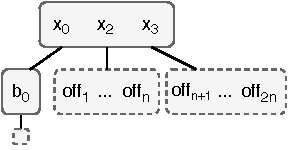
\includegraphics{colt.pdf}
  \caption{A \COLT for the relation $S$ in
    Fig.~\ref{fig:clover-query}. Each off$_i$ is an integer
    representing an offset into the table $S$.}
  \label{fig:colt}
\end{figure}

A \COLT tree need not be balanced, and there can be both hash maps and
vectors at the same tree level.  Fig.~\ref{fig:colt}
illustrates a \COLT tree for the instance $S$ of the clover query
$Q_\clubsuit$.

%%% \begin{ex}\label{ex:colt}
%%%   Recall the relation $S$ for the clover query $Q_\clubsuit$, 
%%%   whose \GHTs are shown in Figure~\ref{fig:ght-examples}.
%%%   Figure~\ref{fig:colt} shows a \COLT for $S$.
%%% \end{ex}


\begin{figure}
  \begin{lstlisting}
struct COLT {
  relation, schema, vars, 
  data = Map(HashMap<Tuple, COLT>) | Vec<Vec<u64>> }

impl GHT for COLT:
  fn new(relation, schema):
    COLT { relation, schema, schema[0],
           data = [ 0, 1, ..., relation.len - 1 ] }

  fn iter():
    match self.data:
      Map(m) => m.keys().iter(),
      Vec(v) => 
          if is_suffix(self.vars, relation.schema):
            v.map(|i| cols = self.relation[self.vars];
                      cols.map(|c| c[i]) )
          else: self.force(); self.iter()

  fn get(key): self.force(); self.get_map.get(key)

  fn force():
    match self.data:
      Map(m) => {} # already forced, do nothing
      Vec(v) => 
        map = new()
        for i in v:
          cols = self.relation[self.vars]
          k = cols.map(|col| col[i])
          if map[k] is None: # make a new, empty COLT
            map[k] = COLT { relation: self.relation, 
                            schema: self.schema[1..], 
                            data: [] }
          map[k].data.push(i)
        self.data = Map(map)
\end{lstlisting}
  \caption{The \COLT data structure.}
  \label{fig:colt-impl}
\end{figure}

% \ds{I did not understand the rest of this section.  What is needed:
%   (a) explain how the raw data is stored.  For example, how is a
%   relation $R(x,y,z)$ stored: row-wise? column-wise? sorted? (b) where
%   are the indices pointing to?  For example, if I construct the first
%   level of $R(x,y,z)$, then for each value of $x$ I have a set of
%   indices: where are these indices pointing to?}
% \rw{I added an example to explain this.}

\COLT Implements the \GHT interface in Figure~\ref{fig:ght}, and its
implementation is shown in Figure~\ref{fig:colt-impl}. As before,
\COLT stores a reference to the relation it represents, as well as the
\GHT schema computed from the plan.
%%% Recall the $i$-th element of the schema contains the variables at
%%% the $i$-th level of the trie.  For a (sub-)\COLT at level $k$,
%%% \lstinline|vars| is the same as the $k$-th element of the
%%% schema. the $0$-th element of the schema.
Consider a relation with $n$ tuples.  The \COLT tree is initialized
with a single node consisting of the vector $[0, \ldots, n-1]$,
i.e. one offset to each tuple.  
\COLT
implements the \lstinline|get| and \lstinline|iter| methods lazily.  
When
\lstinline|get| is called, we check if the current node is a hash
map or a vector.  In the first case, we simply perform a lookup in the
map.  In the second case, we first replace the current vector with a
hash map, whose children are vectors of offsets.  Notice that this
requires iterating over the current vector of offsets, accessing the
tuple in the base table, inserting the key in the hash map, and
inserting the offset in the corresponding child.  Consider now a call
to \lstinline|iter|.  If the current node is a hash map, then we
return an iterator over it.  If it is a vector, then we check if it is
a suffix of the relation schema: if yes, then we simply iterate over
that vector (and access the tuples via their offsets), otherwise we
first materialize the current hash map as explained above, and return
an iterator over the hash map.

As a simple but effective optimization, we do not initialize the \COLT
tree to the single node $[0,1,\ldots,n-1]$, but instead iterate
directly over the base table, if required.  If no \lstinline|get|
is performed on this table, then we have completely eliminated the
cost of building any auxiliary structure on this table.  Thus, the \FJ
plan can be equivalent to a left-deep plan that avoids building a hash
table on the left-most relation.  \COLT is also closer to the structure of
traditional hash tables, which, in some implementations, map a key to
a vector of pointers to tuples.
%
%%% Note that the \COLT for each relation of size $n$ is always initialized to be the 
%%%   vector $[0, \ldots, n-1]$.
%%% Since we can only iterate over this vector, 
%%%   we did not have to materialize it in the first place.
%%% Instead, we can simply loop over the tuples in the original relation 
%%%   when \lstinline|iter| is called.
%%% This means when the \FJ plan is equivalent to a binary plan, 
%%%   we completely eliminate the cost of trie building for the left relation, 
%%%   recovering the behavior of binary join.
%
%%% \COLT also captures the structure of hash tables more closely than
%%% \GHTs.  Recall that a hash table maps each key to an entire tuple in
%%% the relation.  Equivalently, we can also map the key to the row index
%%% of the tuple.  But that is precisely a \COLT whose first level is
%%% materialized.

\begin{ex}\label{ex:colt-clover}
Consider an extension of the clover query $Q_\clubsuit$:
\begin{align*}
  Q(x, a, b, c) \cd R(x,a), S(x,b), T(x, c), \underline{U(b)}.
\end{align*}
  % 
%   \begin{lstlisting}[
%     language=SQL,
%     showspaces=false,
%     basicstyle=\ttfamily\small,
%     commentstyle=\color{gray},
%     escapeinside={(*}{*)},
%  ]
% SELECT * FROM R,S,T,U -- schema: R(x,a),S(x,b),T(x,c),U(b)
%  WHERE R.x = S.x AND S.x = T.x AND T.x = R.x AND (*\underline{S.b = U.b}*)
% \end{lstlisting}
%
\GJ builds a 2-level hash trie for each of $R$, $S$, and $T$, as well
as a 1-level hash trie for $U$.  Consider the \FJ plan
$[[R(x,a),S(x),T(x)],[U(b),S(b)],[T(c)]]$.  \FJ executes the first
node of the plan by iterating over $R$ directly, without constructing
any auxiliary structure. For each tuple $(x, a)$ in $R$, it looks up
$x$ in $S$ and $T$.  Upon the first lookup, \COLT builds the first
level of the \GHT for $S$ and $T$, i.e. a hash map indexed by the $x$
values.  Assuming the database instance for $R,S,T$ shown in
Fig.~\ref{fig:clover-query}, the result of $R.x \cap S.x \cap T.x$ has
only one value, $x_0$, thus, $\FJ$ executes the second node for only
one value $x_0$.  Here it needs to intersect $U(b)$ and $S(b)$.
Assume for the moment that \FJ chooses $U(b)$ to be the cover, on the
first lookup in $S$, \COLT will expand the second level, arriving at
Figure~\ref{fig:colt}: notice that all other $b$ values in $S$ will
never be inserted in the hash table.  More realistically, \FJ follows
the principle in \GJ and chooses $S(b)$ as cover, because it is the
smallest: it builds a hash map for $U$, but none for the 2nd level of
$S$.
\end{ex}

The example highlights a divergence between \GJ and traditional plans.
To intersect $R_1.x \cap R_2.x \cap \ldots$, \GJ choose to iterate
over the smallest relation, which results in the best runtime {\em
  ignoring} the build time.  A traditional join plan will iterate over
the largest relation, because then it needs to build hash tables only
on the smaller relations.  Currently, we follow \GJ, and plan to
explore alternatives in the future.

% \ds{Remy please check the example and the discussion}


% \ds{The example doesn't help.  Once we have identified the single
%   value $b_0$, we only need to look it up in $U(b)$.  But since we
%   haven't constructed anything for $U$ yet, this requires a full scan
%   of $U$.  This is modestly better than scanning $U$ to create a
%   hash-table, but I don't see how this savings generalizes.  If the
%   previous joins return the values $b_0, b_1, b_2, \ldots$, then how
%   can we look them up in $U$ more efficiently than computing a hash
%   table on $U$?}
% \rw{Scanning $U$ while probing into the small trie is much faster than 
% building a hash table for $U$, since the latter needs to allocate memory.
% But the main point is not about $U$, but rather we avoid building a large 
% part of the second level of $S$.  }

\subsection{Vectorized Execution}\label{sec:vectorized-execution}
The \FJ algorithm as presented in Figure~\ref{fig:fj-algo}
  suffers from poor temporal locality.
In the body of the outer loop, 
  we probe into the same set of relations for each tuple.
However, these probes are interrupted by the recursive 
  call at the end, 
  which is itself a loop interrupted by further recursive calls.

\begin{figure}
  \begin{lstlisting}
@outer for ts in tries[0].iter_batch(batch_size):
  tup_subtries = [(tuple + t, [ tries[0].get(t) ]) | t $\in$ ts]
  for trie in tries[1..]:
    for (tup, subtries) in tup_subtries:
      subtrie = trie.lookup(tup[trie.vars])
      if subtrie is None:
        tup_subtries.remove((tup, subtries))
      else: subtries.append(subtrie)
  for (tup, subtries) in tup_subtries:
    new_tries = all_tries[tries $\mapsto$ subtries]
    join(new_tries, plan[1:], tup)
\end{lstlisting}
  \caption{Vectorized execution for \FJ.}
  \label{fig:vectorized-execution}
\end{figure}

A simple way to improve locality is to perform a batch of probes 
  before recursing, just like the classic vectorized execution 
  for binary join.
Concretely, we replace the \lstinline|iter| method 
  with a new method \lstinline|iter_batch(batch_size)|
  which returns up to \lstinline|batch_size| tuples at a time.
If there are less than \lstinline|batch_size| tuples left, 
  it returns all the remaining tuples.
Then we replace the outer loop in Figure~\ref{fig:fj-algo} 
  with the one in Figure~\ref{fig:vectorized-execution}.
For each batch of tuples, 
  we create a vector pairing each tuple to its subtrie in 
  \lstinline|tries[0]|.
Then for each trie to be probed,
  we iterate over the vector and look up each tuple 
  from the trie.
If the lookup succeeds, we append the subtrie to the vector of tries paired with the tuple.
If it fails, we remove the tuple to avoid probing it again.
Finally, with each tuple and the subtries it pairs with, 
  we recursively call \lstinline|join|.

\subsection{Discussion}\label{sec:fj-gj-multijoin}

\COLT is a lazy data structure, sharing a similar goal with database
cracking~\cite{DBLP:conf/cidr/IdreosKM07,DBLP:conf/sigmod/IdreosKM07}, where an
index is constructed incrementally, by performing a little work during each
lookup. 
% \rw{Dan, can you check the following?}
Another connection is to Factorized Databases~\cite{DBLP:journals/sigmod/OlteanuS16} -- we
intentionally used the term ``factor'' when describing how we optimize \FJ plans to
suggest this connection. 
Concretely, we can view the trie data structure as a
factorized representation of a relation, where keys of the same hash map are
combined with union, and tuples are formed by taking the product of values at
different levels. Practically, we can use this factorized representation to 
compress large outputs, saving time and space during materialization.

As we discussed at the end of Section~\ref{sec:free-join}, in order
match the optimality of \GJ, the \FJ algorithm needs to choose
dynamically the ``cover'', i.e. the relation over which to iterate.  To
achieve this, we first find {\em all} covers for each node, then make a simple
change to the \FJ algorithm in Figure~\ref{fig:fj-algo}: we simply
choose to iterate over the cover whose trie has the fewest keys.  For
that we insert the following code right before the outer loop in
Figure~\ref{fig:fj-algo}:
%
\begin{lstlisting}
trie[0] = covers(plan[0]).min_by(|t| t.keys().len)
trie[1..] = # the rest of the tries
\end{lstlisting}
%
When we use \COLTs, we cannot know the exact number of keys in a vector unless
  we force it into a hash map. In that case we use the length of the vector as
  an estimate.

\begin{ex}
  Consider the triangle query $Q_\triangle$, and the following \FJ plan:
  $$[[R(x), T(x)], [R(y), S(y)], [S(z), T(z)]]$$  Each subatom is a
  cover of its own node.  On the outermost loop, we iterate over $R$
  if it has fewer $x$ values, and otherwise we iterate over $T$.  On
  the second loop level we make a decision picking between $S$ and a
  subtrie of $R$, \emph{for each subtrie of $R$}.  Finally, on the
  innermost loop we pick between the subtries of $S$ and $T$.
\end{ex}

% \ds{I recommend removing the paragraph below}
% Another small tweak allows \FJ to further capture other classic
% multiway joins. Just like how \GJ dynamically choose the relation to iterate
% over, various classic multiway joins, such as Hash Team~\cite{} and Eddies~\cite{},
%  also dynamically orders the relations to
% probe into. We support this by inserting another line right before the 
% inner loop of Figure~\ref{fig:fj-algo}:
% %
% \begin{lstlisting}
% tries[1..].sort_by(probe_cost)
% \end{lstlisting}
% %
% Here \lstinline|probe_cost| estimates the cost of probing into each trie.
% The simplest cost function returns the size of the trie;
% a more advanced one may perform some form of selectivity estimation;
% and a sophisticated cost model can even receive feedback from previous 
% iterations of the loop.

\section{Experiments}\label{sec:eval}

% \ds{The section looks good overall.  I made only stylistic changes,
%   mostly in the beginning.  Regarding the Latex layout, I don't
%   onecolumn should be the solution, but instead you should use a
%   figure$*$, then subfigures.  Also, I think you can squeeze in
%   another graph, i.e. arrange them $3 \times 3$.}

We implemented \FJ as a standalone Rust library.  The main entry point
of the library is a function that takes a binary join plan (produced
and optimized by DuckDB), and a set of input relations.  The system
converts the binary plan to a \FJ plan, optimizes it, then runs it
using \COLT and vectorized execution.
%%% The binary plan can be produced by any query optimizer, and we
%%% convert the binary plan into a \FJ plan and further optimize it as
%%% described in Section~\ref{sec:bj-to-fj}.
% In addition to joins, our implementation supports 
%   projection and aggregation, 
%   but relies on an external system for selection.
We compare \FJ against two baselines: our own \GJ implementation in
Rust, and the binary hash join implemented in the state-of-art
in-memory database
DuckDB~\cite{DBLP:conf/cidr/RaasveldtM20,DBLP:conf/vldb/Raasveldt22}.
We evaluate their performance on the popular Join Order Benchmark
(JOB)~\cite{DBLP:journals/pvldb/LeisGMBK015} and the LSQB
benchmark~\cite{DBLP:conf/sigmod/MhedhbiLKWS21}.  
In addition, we compare against K\`uzu~\cite{kuzu:cidr}, 
 a system that implements \GJ.
K\`uzu is the current iteration of the Graphflow system~\cite{DBLP:journals/pvldb/MhedhbiS19}.
We ask three research questions:
\begin{enumerate}
    \item How does \FJ compare to binary and \GJ, on acyclic and cyclic queries?
    \item What is the impact of \COLT and vectorization on \FJ?
    \item How sensitive is \FJ to the query optimizer's quality?
\end{enumerate}

% \clearpage
% \onecolumn
\subsection{Setup}

While we had easy access to optimized join plans produced by DuckDB,
we did not find any system that produces optimized \GJ plans, 
or can take an optimized plan as input.
%%% 
%%% In addition to using DuckDB as a baseline implementation of binary
%%% join, we use its query optimizer to generate the starting binary plan
%%% that we convert into a \FJ plan.
%%% %
%%% Compared to binary join implementations, 
%%%   there are few systems that implement \GJ, 
%%%   and none of them outputs a machine-readable query plan,
%%%   or can take one as input.
We therefore implement a \GJ baseline ourselves,
by modifying \FJ to fully construct all tries, and removing
vectorization.  We chose as variable order for \GJ the same as for
\FJ.\footnote{\FJ defines only a partial order; we extended it to a
  total order.}

%%% It is essentially \FJ but without the optimizations:
%%%   its execution is not vectorized, and
%%%   instead of using \COLT, it fully constructs every trie ahead of time.
%%% We are not aware of any other algorithm converting a binary plan into a \GJ plan, 
%%%   so we use the same plan for both \FJ and \GJ to ensure a fair comparison.

Both  the JOB and the LSQB benchmarks  focus on joins.
JOB contains 113 acyclic queries with an average of 8 joins per query,
  whereas LSQB contains both cyclic and acyclic queries.
Each query in the benchmarks only contains base-table filters, 
  natural joins, and a simple group-by at the end,
  and no null values.
JOB works over real-world data from the IMDB dataset, 
  and LSQB uses synthetic data.
We exclude 5 queries from JOB that return empty results, 
  since such empty queries are known to introduce reproducibility issues\footnote{
    See GitHub issue: \url{https://github.com/gregrahn/join-order-benchmark/issues/11}
  }.
We use the first 5 queries from LSQB; the other 4 queries require 
  anti-joins or outer joins which we do not support.

We ran all our experiments on a MacBook Air laptop with Apple M1 chip and 16GB memory. 
All systems are configured to run single-threaded in main memory, 
  and we leave all of DuckDB's configurations to be the default.
All systems are given the same binary plan optimzed by DuckDB.
To answer our third research question, 
  we needed to hijack DuckDB's optimizer to produce a poor plan.
We did this by modifying its cardinality estimator to always return 1.
Since we are only interested in the performance of the join algorithm, 
  we exclude the time spent in selection and aggregation 
  when reporting performance.
This excluded time takes up on average less than 1\% of the total execution time.

\begin{figure*}
  \centering
  \begin{minipage}[t]{.45\textwidth}
    \centering
    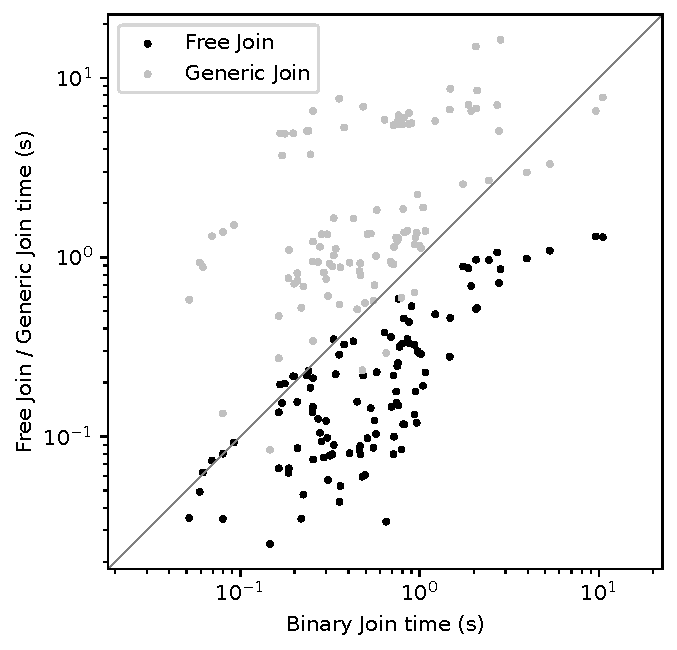
\includegraphics[width=\linewidth]{imdb.pdf}
    \captionof{figure}{Run time comparison on JOB. 
    Each black dot compares the run time of a query on \FJ and binary join, 
    and a black dot below the diagonal means \FJ is faster.
    The gray dots compare \GJ and binary join similarly.
    }
    \label{fig:eval:imdb}
  \end{minipage}%
  \hspace{1em}
  \begin{minipage}[t]{.45\textwidth}
    \centering
    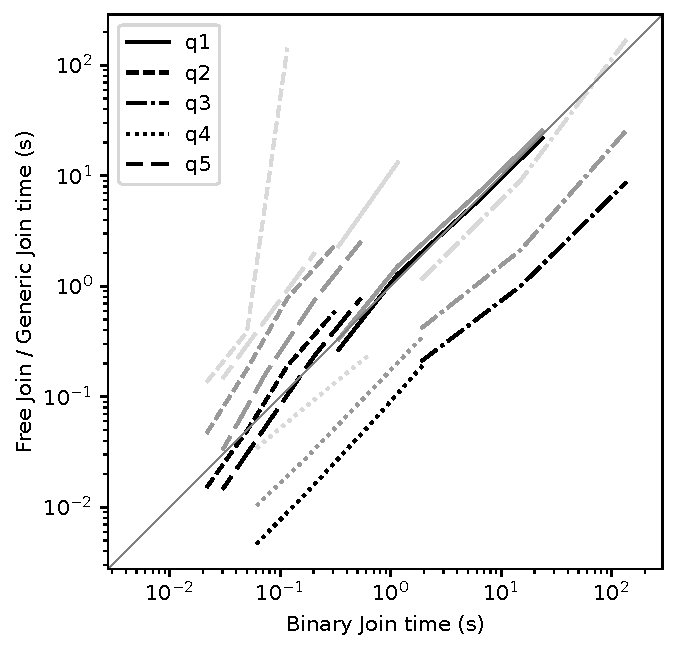
\includegraphics[width=\linewidth]{lsqb-slow.pdf}
    % \captionof{figure}{\FJ and \GJ v.s.\ binary join on LSQB queries.
    % Each line is a query running on increasing scaling factors (0.1-3).
    % Grey lines are for \GJ, and black lines are for \FJ.
    % }
    \captionof{figure}{Run time comparison on LSQB.
    Each line is a query running on increasing scaling factors (0.1, 0.3, 1, 3).
    The black lines compare \FJ with binary join, 
     the gray lines compare our \GJ baseline with binary join, 
     and the light gray lines compare K\`uzu with binary join.
    }
    % Grey lines are for \GJ, and black lines are for \FJ.
    % }
    \label{fig:eval:lsqb}
  \end{minipage}
  \end{figure*}


\subsection{Run time comparison}\label{sec:run-time-comparison}
Our first set of experiments compare the performance of \FJ, \GJ, and binary join
  on the JOB and LSQB benchmarks.
For each query in the benchmarks, we invoke DuckDB to obtain an optimized binary plan,
  and provide the plan to our \FJ and \GJ implementation.
We run LSQB with the scaling factors 0.1, 0.3, 1, and 3, 
  as some queries run out of memory with larger scaling factors.

Figure~\ref{fig:eval:imdb} compares the run time of \FJ and \GJ against binary join on JOB queries.
We see that almost all data points for \FJ are below the diagonal, 
  indicating that \FJ is faster than binary join.
On the other hand, the data points for \GJ are largely above the diagonal, 
  indicating that \GJ is slower than both binary join and \FJ.
On average (geometric mean), \FJ is \imdbavgfjbj faster than binary join 
  and \imdbavgfjgj faster than \GJ.
The maximum speedups of \FJ against binary join and \GJ 
  are \imdbmaxfjbj and \imdbmaxfjgj, respectively, 
  while the minimum speedups are \imdbminfjbj (\imdbmaxbjfj slowdown) and \imdbminfjgj.

We zoom in onto a few interesting queries for a deeper look.
The slowest query under DuckDB is Q13a, taking over 10 seconds to finish.
  \GJ runs slightly faster, taking 7 seconds, 
  whereas \FJ takes just over 1 second.
The query plan for this query reveals the bottleneck for binary join:
  the first 3 binary joins are over 4 very large tables, 
  and two of the joins are many-to-many joins, exploding the 
  intermediate result to contain over 100 million tuples.
However, all 3 joins are on the same attribute;
in other words they are quite  similar to our clover query $Q_\clubsuit$.
As a result, \GJ and \FJ simply intersects the relations 
  on that join attribute, 
  expanding the remaining attributes only after 
  other more selective joins.
This data point appears to confirm a folklore that claims
  \WCOJ algorithms are more resistant to poor query plans.
After all, binary join could have been faster, had the query plan 
  ordered the more selective joins first.
We expand on this point with more experiments evaluating 
  each algorithm's robustness against poor plans in Section~\ref{sec:robustness}.

On a few queries \FJ runs slightly slower than binary join, 
  as shown by the data points over the diagonal.
The binary plans for these queries are all bushy, 
  and each query materializes a large intermediate relation.
We have not spent much effort optimizing for materialization, 
  and we implement a simple strategy: for each intermediate 
  that we need to materialize, we store the tuples containing 
  all base-table attributes in a simple vector.
Future work may explore more efficient materialization strategies, 
  for example only materializing attributes that 
  are needed by future joins.


Figure~\ref{fig:eval:lsqb} compares the performance of \FJ and \GJ against binary join on LSQB queries.
Each line corresponds to one query running on scaling factors 0.1, 0.3, 1, and 3.
The black lines are for \FJ, gray lines for our own \GJ baseline, and light gray lines for K\`uzu.
K\`uzu errors when loading data for SF3;
it did not finish after 10 minutes for q1 SF 1. 
DuckDB also took over 10 minutes running q3 SF 3. 
These instances do not show up in the figure.
We can see K\`uzu takes consistently longer than our \GJ implementation
 on all queries across scaling factors.
This shows that our \GJ implementation is a reasonable baseline to compare against.
On cyclic queries, \FJ is up to 15.45x (q3) faster than binary join, 
  and up to 4.08x (q2) faster than \GJ.
On acyclic queries \FJ is up to 13.07x (q4) and 3.25x (q5) faster than binary join and \GJ, respectively.
On q3 and q4 both \FJ and \GJ consistently outperform binary join on all scaling factors.
q3 contains many cycles, whereas q4 is a star query, so the superior performance of \FJ and \GJ is expected.
% q1, however, is a chain query, where \WCOJ algorithms are expected to be inefficient.
% A deeper look reveals q1 to have an output much larger than its inputs, 
%   but uses a \lstinline|COUNT(*)| at the top.
% An unintended benefit of \GJ and \FJ is that any attributes that 
%   do not participate in a join are not expanded, 
%   so the output result is naturally stored in a \emph{factorized} form.
% We compute the \lstinline|COUNT| aggregate directly on the factorized output, 
%   which is much faster than expanding and counting.
Surprisingly, despite q2 being a cyclic query, 
  \FJ is only slightly faster on smaller inputs
  and is even slightly slower on larger inputs.
This is the opposite of the common believe that \WCOJ algorithms
  should be faster on cyclic queries.
The query plan reveals that there are no skewed joins,
  and so binary join suffers no penalty.
Our experience shows that, in practice, 
  the superiority of \WCOJ algorithms like \FJ and \GJ
  is not solely determined by the cyclicity of the query;
  the presence of skew in the data is another important factor.

\begin{figure}
  \centering
  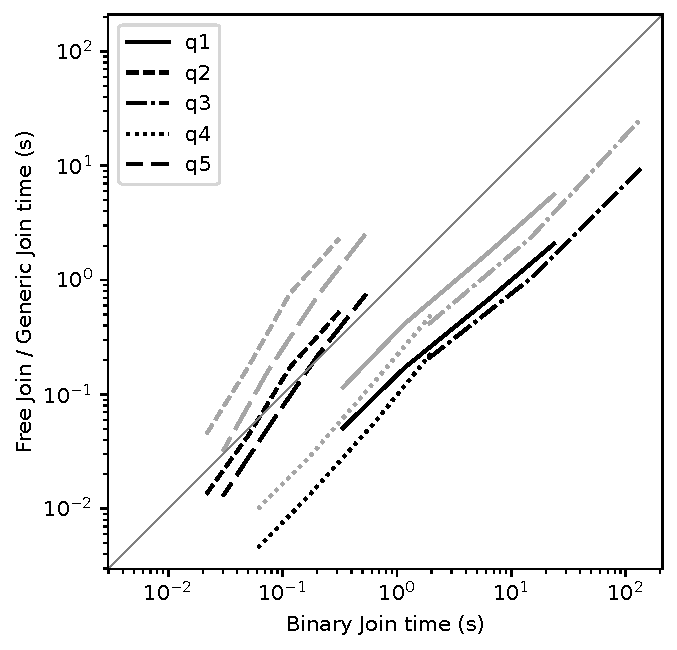
\includegraphics[width=.45\linewidth]{lsqb.pdf}
  \caption{Run time comparison on LSQB w/ factorization.}
  \label{fig:eval:lsqb-factor}
\end{figure}

Unlike the JOB queries, in LSQB the output size (before aggregation)
  is much larger than the input size.
This leads to a large amount of time spent in constructing the output, 
  which involves random accesses to retrieve the data values for each tuple.
We therefore implemented the optimization in Section~\ref{sec:fj-gj-multijoin}
  to factorize the output.
This made q1 significant faster, as shown in Figure~\ref{fig:eval:lsqb-factor},
  while other queries are not affected.

\begin{figure*}
  \centering
  \begin{minipage}{.45\textwidth}
    \centering
    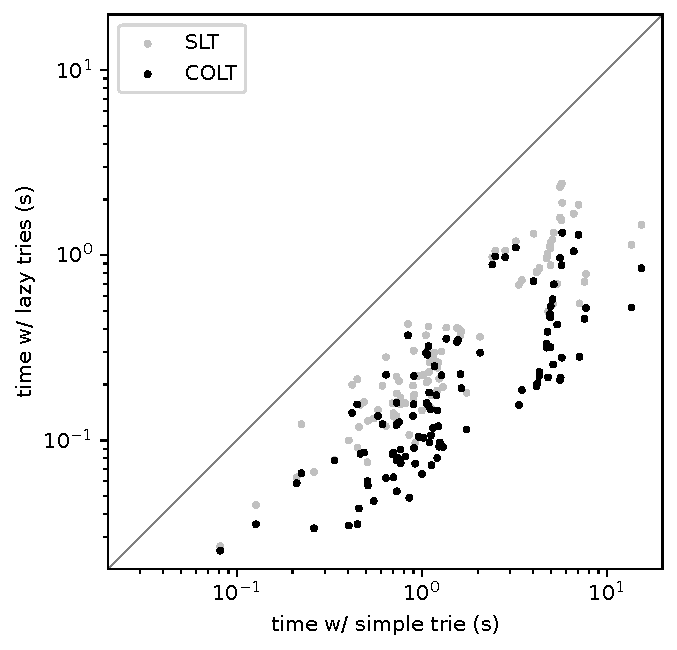
\includegraphics[width=\linewidth]{colt-ab.pdf}
    \captionof{figure}{Impact of \COLT.}
    \label{fig:eval:colt-ab}
  \end{minipage}%
  \hspace{1em}
  \begin{minipage}{.45\textwidth}
    \centering
    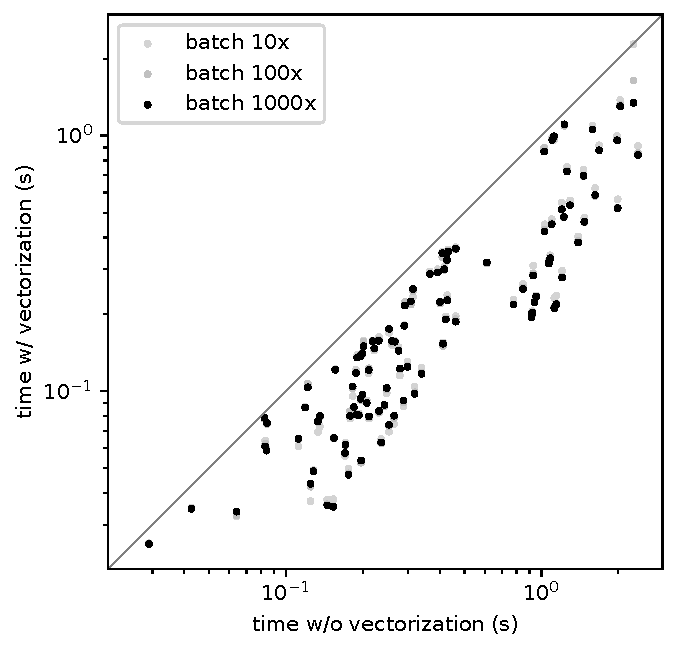
\includegraphics[width=\linewidth]{vec-ab.pdf}
    \captionof{figure}{Impact of vectorization.}
    \label{fig:eval:vec-ab}
  \end{minipage}
  \end{figure*}
  \subsection{Impact of \COLT and Vectorization}
  % \ds{Try to choose section titles that are related to the question
  %   that the section addresses}
The three key ingredients that make \FJ efficient 
  are \begin{enumerate*}
    \item our algorithm to optimize the \FJ plan by factoring,
    \item the \COLT data structure, and
    \item the vectorized execution algorithm.
  \end{enumerate*}
We conduct an ablation study to evaluate the performance impact of these components. 
But if we do not optimize the \FJ plan converted from a binary plan 
  and execute it as-is, \FJ would behave identically to binary join.
Since we have already compared \FJ with binary join in Section~\ref{sec:run-time-comparison},
  we do not repeat it here.
Therefore, our ablation study includes two sets of experiments, 
  evaluating the impact of \COLT and vectorization respectively.



Figure~\ref{fig:eval:colt-ab} compares the run time of \FJ using different trie data structures.
The baseline fully expands each trie ahead of time, and we call this \emph{simple trie}.
Another data structure, \emph{simple lazy trie} (SLT), expands the first level of each trie 
  ahead of time, while expanding the inner levels lazily.
This is the same strategy as proposed by~\cite{DBLP:journals/pvldb/FreitagBSKN20}.
Finally, \COLT is our column-oriented lazy trie.
In all three cases, we use the default vectorization batch size 1000.
The experiments show the average (geometric mean) speedup of \COLT 
  is 1.91x and 8.47x, over SLT and simple trie respectively,
  and the maximum speedup over them is 11.01x and 26.29x, respectively.


Figure~\ref{fig:eval:vec-ab} compares the run time of \FJ using different vectorization batch sizes.
The baseline uses no vectorization, i.e., we set the batch size to 1.
Then we adjust the batch size among 10, 100, and 1000.
The data does not show significant performance differences among
  the different batch sizes -- 
  it appears \emph{any amount of vectorization is better than none}.
For short-running queries, a smaller batch size perform slightly better,
  and for longer running queries a larger batch size wins.
We conjecture this is due to a smaller batch having less overhead, 
  leading to lower latency, 
  while a larger batch size speeds up large joins better,
  leading to better throughput. 
Overall, using the default batch size 1000
  leads to an average (geometric mean) speedup of 2.12x, 
  and a maximum speedup of 5.33x over non-vectorized \FJ.

\begin{figure*}
\begin{minipage}{.48\linewidth}
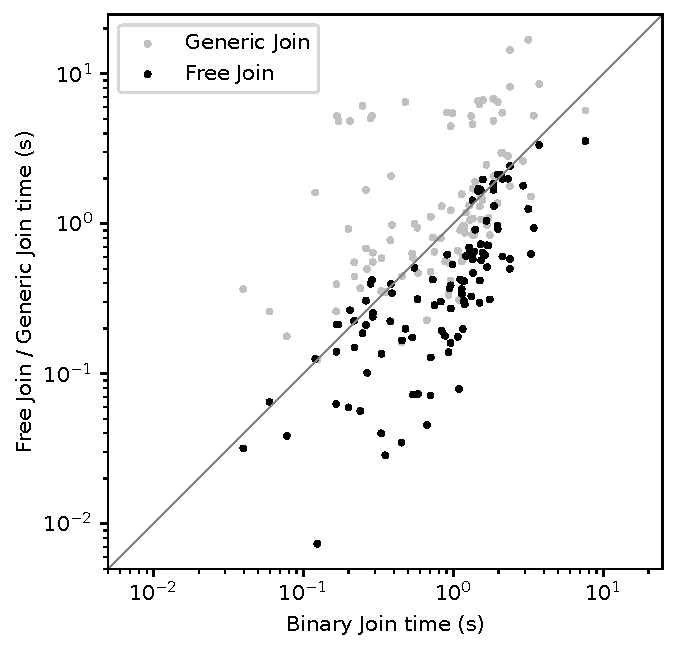
\includegraphics[width=\linewidth]{robust.pdf}
\end{minipage}
\begin{minipage}{.48\textwidth}
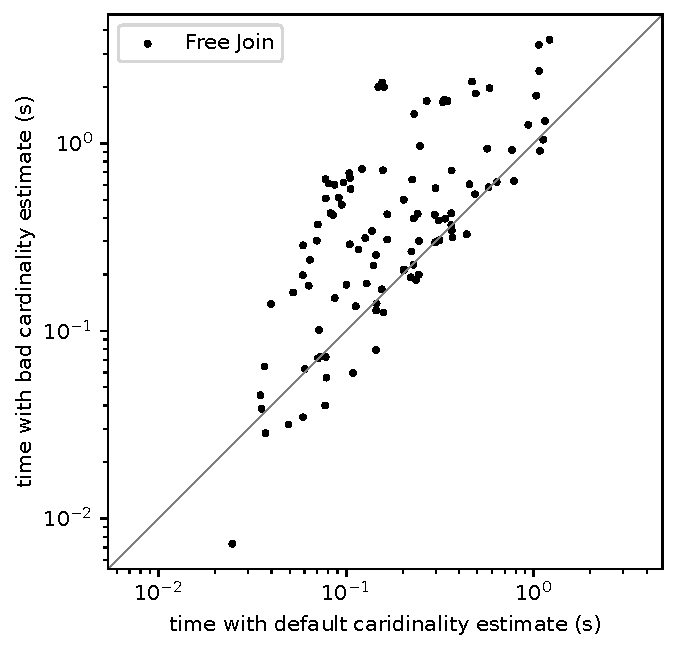
\includegraphics[width=\linewidth]{robust_fj.pdf}
\end{minipage}

\begin{minipage}{.48\textwidth}
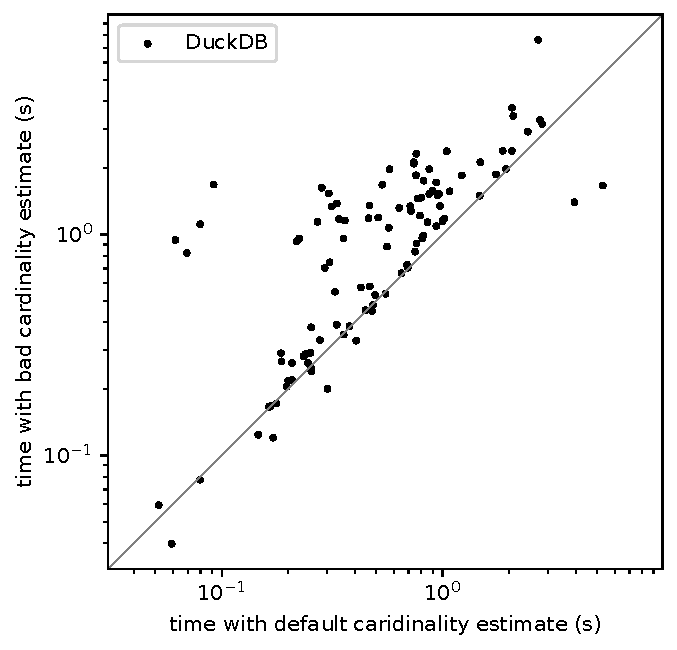
\includegraphics[width=\linewidth]{robust_bj.pdf}
\end{minipage}
\begin{minipage}{.48\textwidth}
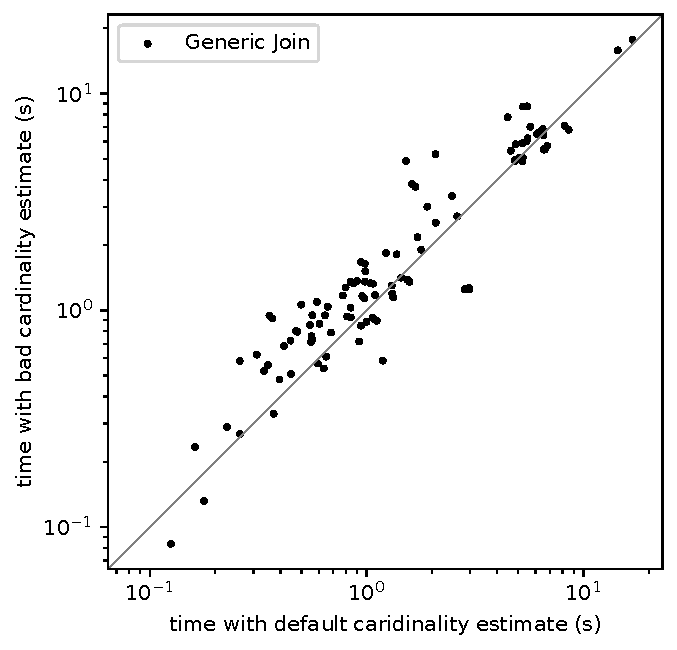
\includegraphics[width=\linewidth]{robust_gj.pdf}
\end{minipage}
\caption{Run time of join algorithms with good and bad cardinality estimates.
The first plot compares the run time of \FJ, \GJ and binary join
  on JOB with bad cardinality estimates.
The remaining three plots compare the run time of each algorithm 
with good and bad cardinality estimates on JOB.
}
\label{fig:sensitivity}
\end{figure*}

\subsection{Robustness Against Poor Plans}\label{sec:robustness}

Our last set of experiments compares \FJ, \GJ and binary join 
  on their sensitivity to the quality of the query plan.
Many believe \WCOJ algorithms suffer less from poor query planning,
  due to its asymptotic guarantees.
Our experience with Q13 from Section~\ref{sec:run-time-comparison}
  also seems to confirm this intuition.
However, our experimental results tell a different story.
As the first plot in Figure~\ref{fig:sensitivity} shows, 
  the relative performance of the three algorithms stays 
  the same with good and bad plans, with \FJ being the fastest,
  \GJ the slowest, and binary join in the middle.
However, as shown in Figure~\ref{fig:sensitivity},
  \FJ seems to slow down as much as binary join 
  when the plan is bad (there are many points far above the diagonal).
It turns out with a poor cardinality estimate, 
  DuckDB routinely outputs bushy plans that materialize large results.
We have noted in Section~\ref{sec:run-time-comparison} that 
  our materialization strategy is simplistic, 
  so with larger intermediates it leads to more severe slowdown.
In comparison, \GJ slows down less (the data points are close to the diagonal).
However, it was the slowest to begin with,
  and since overheads like trie building dominates \GJ's run time, 
  a bad plan does not make it much slower.
Overall, we believe \FJ can be more robust to bad plans with 
  faster materialization.

\chapter{Optimizing Nonrecursive Queries}
\label{chapter:spores}


Consider the Linear Algebra (LA) expression $sum((X-UV^T)^2)$ which
defines a typical loss function for approximating a matrix $X$ with a
low-rank matrix $UV^T$. Here, $sum()$ computes the sum of all matrix
entries in its argument, and $A^2$ squares the matrix $A$
element-wise. Suppose $X$ is a sparse, 1M x 500k matrix, and suppose
$U$ and $V$ are dense vectors of dimensions 1M and 500k respectively.
Thus, $UV^T$ is a rank 1 matrix of size 1M x 500k, and computing it
naively requires 0.5 trillion multiplications, plus memory allocation.
Fortunately, the expression is equivalent to
$sum(X^2) - 2U^TXV + U^TU * V^TV$.  Here $U^TXV$ is a scalar that can
be computed efficiently by taking advantage of the sparsity of $X$,
and, similarly, $U^TU$ and $V^TV$ are scalar values requiring only 1M
and 500k multiplications respectively.

Optimization opportunities like this are ubiquitous in machine
learning programs. State-of-the-art optimizing compilers such as
SystemML~\cite{DBLP:reference/bdt/Boehm19},
OptiML\cite{DBLP:conf/icml/SujeethLBRCWAOO11}, and
Cumulon\cite{DBLP:conf/sigmod/HuangB013} commonly implement syntactic
rewrite rules that exploit the algebraic properties of the LA
expressions. For example, SystemML includes a rule that rewrites the
preceding example to a specialized operator\footnote{See the
  \href{https://systemml.apache.org/docs/0.12.0/engine-dev-guide.html}{SystemML
    Engine Developer Guide} for details on the weighted-square loss
  operator \texttt{wsloss}. } to compute the result in a streaming
fashion.  However, such syntactic rules fail on the simplest
variations, for example SystemML fails to optimize $sum((X+UV^T)^2)$,
where we just replaced $-$ with $+$.  Moreover, rules may interact
with each other in complex ways.  In addition, complex ML programs
often have many common subexpressions (CSE), that further interact
with syntactic rules, for example the same expression $UV^T$ may occur
in multiple contexts, each requiring different optimization rules.

In this chapter we describe \sys, a novel optimization approach for
complex linear algebra programs that leverages relational algebra as
an intermediate representation to completely represent the search
space. SPORES first transforms LA expressions into traditional
Relational Algebra (RA) expressions consisting of joins, unions 
and aggregates.  It then performs a cost-based optimizations on
the resulting Relational Algebra expressions, using only standard
identities in RA.  Finally, the resulting RA expression is converted
back to LA, and executed.

A major advantage of \sys\ is that the rewrite rules in RA are
complete.  Linear Algebra seems to require an endless supply of clever
rewrite rules, but, in contrast, by converting to RA, we can prove
that our set of just 13 rules are complete. The RA expressions in this dissertation are
over $K$-relations~\cite{DBLP:conf/pods/GreenKT07}; a tuple $X(i,j)$
is no longer true or false, but has a numerical value, e.g. $5$,
%
which could be interpreted, e.g., as the multiplicity of that tuple.
%
In other words, the RA expressions that result from LA expressions are
interpreted over bags instead of sets. 
\rvo{The problem of checking equivalence of
queries under bag semantics has a unique history.  Chaudhuri and Vardi
first studied the containment and equivalence problem under bag
semantics, and claimed that two conjunctive queries are equivalent iff
they are isomorphic: Theorem 5.2
in~\cite{DBLP:conf/pods/ChaudhuriV93}.  However, a proof was never
produced.  A rather long proof for this claim was given for the
bag-set semantics in~\cite{DBLP:journals/tocl/CohenSN05}.  Green
provided a comprehensive proof, showing that two unions of conjunctive
queries (UCQ) are equivalent under bag semantics iff they are
isomorphic, by using sophisticated techniques involving multiple
semirings~\cite{DBLP:conf/icdt/Green09}.  The completeness result of
our 13 rules relies on a similar result, but stated for tensors rather
than bags; we present here a simple and self-contained proof in
Sec.~\ref{ranf}.  We note that, in contrast, {\em containment} of two
UCQs with bag semantics is
undecidable~\cite{DBLP:journals/tods/IoannidisR95}; we do not consider
containment in this dissertation.
}
Finally, we prove that our optimizer rules are
sufficient to convert any RA expression into its {\em canonical form},
i.e.  to an UCQ, and thus can, in principle, discover all equivalent
rewritings.

However, we faced a major challenge in trying to exploit the
completeness of the rules.  The search space is very large,
typically larger than that encountered in standard database
optimizers, because of the prevalence of unions $+$, large number of
aggregates $\sum$, and frequent common subexpressions. To tackle this,
\sys\ adopts and extends a technique from compilers called {\em
  equality saturation}~\cite{DBLP:journals/corr/abs-1012-1802}.
It uses a data structure called the E-Graph \cite{10.5555/909447} to
compactly represent the space of equivalent expressions, and equality
rules to populate the E-Graph, then leverages constraint solvers to
extract the optimal expression from the E-Graph. \rvo{We extend equality
saturation with rule sampling and use a greedy extraction algorithm
to quickly cover vast portions of the search space, and trade the
guarantee of optimality for shorter compile time.} 

We have integrated \sys\ into
SystemML~\cite{DBLP:reference/bdt/Boehm19}, and show that it can
derive all hand-coded rules of SystemML.  We evaluated \sys\ on a
spectrum of machine learning tasks, showing competitive performance
improvement compared with more mature heuristic-based optimizers. Our
optimizer rediscovers all optimizations by the latter, and also finds
new optimizations that contribute to \rvo{up to 10X speedup}.

We make the following contributions in this dissertation:
\begin{enumerate}
\item We describe a novel approach for optimizing complex Linear
  Algebra expressions by converting them to Relational Algebra, \rvo{and
  prove the completeness of our rewrite rules} (Sec.~\ref{sec:la:to:ra}).
\item We present a search algorithm based on Equality Saturation that
  can explore a large search space while reusing memory (Sec.~\ref{explore}).
\item We conduct an empirical evaluation of the optimizer using
  several real-world machine learning tasks, and demonstrate it's
  superiority over an heuristics-driven optimizer in SystemML
  (Sec.~\ref{sec:evaluation}).
\end{enumerate}{}

\section{Representing the Search Space} \label{sec:la:to:ra}

\subsection{Rules \texorpdfstring{$R_{LR}$}{R\_LR}: from  LA to RA and Back}
In this section we describe our approach of optimizing LA expressions
by converting them to RA.  The rules converting from LA to RA and back
are denoted $R_{LR}$.

To justify our approach, let us revisit our example loss function
written in LA and attempt to optimize it using standard LA identities.
Here we focus on algebraic rewrites and put aside concerns about the
cost model. Using the usual identities on linear algebra expressions,
one may attempt to rewrite the original expression as follows:
\begin{align*}
& sum((X-UV^T)^2) \\
= &sum((X-UV^T)*(X-UV^T)) \\
=&sum(X^2-2X*UV^T+(UV^T)^2) \\
= & sum(X^2) - 2sum(X*UV^T) + sum((UV^T)^2)
\end{align*}
% \dan{$(UV^T)^2$ should be $sum(UV^T)^2$.}
At this point we are stuck trying to rewrite $sum(X*UV^T)$ (recall
that $*$ is element-wise multiplication); it turns out to be equal to
$sum(U^TXV)$, for any matrices $X,U,V$ (and it is equal to the scalar
$U^TXV$ when $U, V$ are column vectors), but this does not seem to
follow from standard LA identities like associativity, commutativity,
and distributivity.  Similarly, we are stuck trying to rewrite
$sum((UV^T)^2)$ to $sum(U^TU * V^TV)$.  Current systems manually add
syntactic rewrite rules, whenever such a special case is deemed
frequent enough to justify extending the optimizer.


\begin{table}
\caption{Representation of expressions in LA and RA.}
\vspace{3pt}
\centering
%%% (Dan: I replaced the multiplicies 1,2 with different ones so
%%% readers don't confuse them with indices in the matrix)
\begin{tabular}{@{}ccccc@{}}
&
     $A$ & $x$ & $A * x^T$ & $Ax$\\
     \hline
     \\[-1em]
LA &
     $\begin{bmatrix}
    0 & 5 \\
    7 & 0
    \end{bmatrix}$ & $\begin{bmatrix}
    3\\
    2
    \end{bmatrix}$ & $\begin{bmatrix}
    0 & 10 \\
    21 & 0
    \end{bmatrix}$ & $\begin{bmatrix}
    10 \\
    21
    \end{bmatrix}$ \\
    \\[-0.8em]
    \hline
RA &
    \begin{tabular}{|c|c|c}
    $i$ &$j$&\# \\
    \hline
        $1$ & $2$ & 5 \\
        $2$ & $1$ & 7
    \end{tabular}{} &
    \begin{tabular}{|c|c}
         $j$ &\# \\
         \hline
         1 & 3\\
         2 & 2
    \end{tabular}{} &
    \begin{tabular}{|c|c|c}
    $i$ &$j$ & \# \\
    \hline
        $1$ & $2$ & 10 \\
        $2$ & $1$ & 21
    \end{tabular}{} &
    \begin{tabular}{|c|c}
         $i$ & \# \\
         \hline
         1 & 10 \\
         2 & 21
    \end{tabular}{} 
\end{tabular}{}
    % \caption{Top: Linear Algebra manipulates matrices and vectors.
%   $A*x^T$ is (broadcasting) element-wise multiplication, computing the matrix
%   $(A_{ij}x_j)_{ij}$, while $Ax$ is standard matrix-vector
%   multiplication.  Bottom: their translations into $K$-relations and
%   Relational Algebra operations.  Each relation is a bag, where the
%   attribute $\#$ represents the multiplicity, i.e. $A(1,2)$ has
%   multiplicity $5$ etc.  Then $A*x^T$ becomes a standard query
%   $Q(i,j) = A(i,j) \times x(j)$, while $Ax$ is a query with a group-by and
%   aggregate, $Q(i) = \sum_j A(i,j) \times x(j)$.}
    \label{matrixkrel}
    \vspace*{8pt}
\end{table}{}

Instead, our approach is to expand out the LA expression element-wise.
For example, assuming for simplicity that $U,V$ are column vectors, we
obtain
\begin{align*}
& sum((UV^T)^2) = \textstyle{\sum_{i,j}} (U_i \times V_j) \times (U_i \times V_j) \\
& = \textstyle{\sum_{i,j}}(U_i \times U_i) \times (V_j \times V_j) \\
& = ( \textstyle{\sum_i} U_i \times U_i) \times ( \textstyle{\sum_j} V_j \times V_j)  \\
& = U^TU \times V^TV
\end{align*}
%
The expressions using indices represent Relational Algebra
expressions.  More precisely, we interpret every vector, or matrix, or
tensor, as a $K$-relation~\cite{DBLP:conf/pods/GreenKT07} over the
reals. In other words we view $X_{ij}$ as a tuple $X(i,j)$ whose
``multiplicity'' is the real value of that matrix element.  We
interpret point-wise multiply as natural join; addition as union; sum
as aggregate; and matrix multiply as aggregate over a join\footnote{In
  the implementation, we use outer join for point-wise multiply and
  addition, where we multiply and add the matrix entries
  accordingly. In this chapter we use join and union to simplify
  presentation.}.
%
Table~\ref{matrixkrel} illustrates the correspondence between LA and
RA.  We treat each matrix entry $A_{ij}$ as the multiplicity of tuple
$(i, j)$ in relation $A$ under bag semantics. For example
$A_{2,1} = 7$, therefore the tuple $(2,1)$ has multiplicity of $7$ in
the corresponding relation. \rvt{The relation schema stores the size of each dimension.}
$A*x^T$ denotes element-wise
multiplication, where each element $A_{ij}$ of the matrix is
multiplied with the element $x_j$ of the row-vector $x^T$.  In RA it
is naturally interpreted as the natural join $A(i,j) \Join x(j)$,
which we write as $A(i,j) \times x(j)$.  Similarly, $Ax$ is the standard
matrix-vector multiplication in LA, while in RA it becomes a query
with a group by and aggregate, which we write as $\sum_j A(i,j) \times x(j)$.
Our $K$-relations are more general than bags, since the entry of a
matrix can be a real number, or a negative number; they correspond to
$K$-relations over the semiring of reals $(\R, 0, 1, +, \times)$.

% Of course, a matrix can have an entry that is not an integer, which
% would not make sense as multiplicity. In general, the matrix entries
% corresponds to the semiring of reals which serve as relation
% annotations \cite{DBLP:conf/pods/GreenKT07} in the $K$-relation.
\begin{table}
\caption{LA and RA operators. The type $M_{M,N}$ is a matrix of size $M \times
  N$; $[i,j]$ is a list of attribute names; $R_{i:M,j:N}$ is a relation with
  attributes $i$ of size $M$ and $j$ of size $N$; $S_1, S_2, S,$ and $U$ are
  sets of attributes. \rvt{\texttt{elemmult} and \texttt{elemplus} are broadcasting.}}
\begin{tabular}{llll}
&name & type & syntax \\ \hline \multirow{7}{*}{\rotatebox[origin=c]{90}{LA}}
  &mmult & $M_{M,L} \times M_{L,N} \rightarrow M_{M,N}$ & $AB$ 
  \\ &elemmult & $M_{M,N} \times M_{M,N} \rightarrow M_{M,N}$ & $A*B$
  \\ &elemplus & $M_{M,N} \times M_{M,N} \rightarrow M_{M,N}$ & $A+B$ \\ &rowagg
  & $M_{M,N} \rightarrow M_{M,1}$ & $sum_{row} A$ \\ &colagg & $M_{M,N}
  \rightarrow M_{1,N}$ & $sum_{col} A$ \\ &agg & $M_{M,N} \rightarrow M_{1,1}$ &
  $sum A$ \\
%&power & $M  \times Int \rightarrow M$ & $A^k$ \\
&transpose & $M_{M,N} \rightarrow M_{N,M}$ & $A^\tr$ \\ \hline
  \multirow{2}{*}{\rotatebox[origin=c]{90}{conv.}} &bind & $M_{M,N} \times [i,j]
  \rightarrow R_{i:M,j:N}$ & $\bind{i,j} A$ \\ &unbind & $R_{i:M,j:N} \times
              [i,j] \rightarrow M_{M,N}$ & $\unbind{i}{j} A$ \\ \hline
              \multirow{2}{*}{\rotatebox[origin=c]{90}{RA}} &join & $R_{S_1}
              \times R_{S_2} \rightarrow R_{S_1 \cup S_2}$ & $A \rmul B$
              \\ &union & $R_{S_1} \times R_{S_2} \rightarrow R_{S_1 \cup S_2}$
              & $A \radd B$ \\ &agg & $R_S \times U \rightarrow R_{S \setminus
                U}$ & $\sum_{U} A$ \\
\end{tabular}

\label{tPlanOps}
\end{table}
\begin{figure}
\begin{enumerate}
\itemsep0em
  \item $A*B \rightarrow \unbind{i}{j}(\bind{i,j}A \rmul \bind{i,j}B)$.
  \item $A+B \rightarrow \unbind{i}{j}(\bind{i,j}A \radd \bind{i,j}B)$.
  \item $sum_{row} A \rightarrow [-i,\_ ] \sum_j \bind{i,j} A$. Similar for
    $sum_{col}$, $sum$.
  \item $AB \rightarrow \unbind{i}{k} \sum_j (\bind{i,j}A \rmul \bind{j,k}B)$.
  \item $A^\tr \rightarrow \unbind{j}{i} \bind{i,j}A$.
  \item $A - B \rightarrow A + (-1) * B$
\end{enumerate}
\caption{LA-to-RA Ruleset $R_{LR}$.}
\vspace*{3pt}
\label{RMR}
\end{figure}

% Following our relational semantics, $sum((X-UV^T)^2)$ is interpreted
% as
% $\sum_{ij} (X_{ij} - U_{i} \bowtie V_{j}) \bowtie (X_{ij} - U_{i}
% \bowtie V_{j})$. Note that because $U$ and $V$ are vectors, the
% aggregate in their matrix product $\sum_{\varnothing} U_i \bowtie V_j$
% is over an empty set of attributes and therefore eliminated.
% Hereafter we will overload $*$ for join and $+$ for union to keep our
% formulas intuitive.  Table~\ref{tPlanOps} provides the list of LA and
% RA operators.  

We now describe the general approach in \sys.  The definition
of LA and RA are in Table~\ref{tPlanOps}.  LA consists of seven
operators, which are those supported in
SystemML~\cite{DBLP:reference/bdt/Boehm19}. \rvt{These operators all 
implement sum-product operations and take up the majority of run
time in machine learning programs as we show in Section~\ref{perf}.
We also support common operations like division and logarithm as we
discuss in Section~\ref{udfs}.} RA consists of only three
operators: $\times$ (natural join), $+$ (union), and $\sum$ (group-by
aggregate).  Difference is represented as $A-B = A + (-1)B$ (this is
difference in $\R$; we do not support bag difference, i.e.  difference
in $\N$ like $3-5=0$, because there is no corresponding operation in
LA), while selection can be encoded by multiplication with relations
with 0/1 entries.  We call an expression using these three RA
operators an {\em RPlan}, for Relational Plan, and use the terms RPlan
and RA/relational algebra interchangeably.  Finally, there are two
operators, {\em bind} and {\em unbind} for converting between
matrices/vectors and $K$-relations.


The translation from LA to RA is achieved by a set of rules, denoted
$R_{LR}$, and shown in Figure~\ref{RMR}. The bind operator
$\bind{i,j}$ converts a matrix to a relation by giving attributes
$i,j$ to its two dimensions; the unbind operator $\unbind{i}{j}$
converts a relation back to a matrix. For example,
$\unbind{j}{i}\bind{i,j}A$ binds $A$'s row indices to $i$ and its
column indices to $j$, then unbinds them in the opposite order,
thereby transposing $A$.

\sys\ translates a complex LA expression into RA by first applying the
rules $R_{LR}$ in Figure~\ref{RMR} to each LA operator, replacing it
with an RA operator, preceded by {\em bind} and followed by {\em
  unbind}. Next, it eliminates consecutive unbind/bind operators,
possibly renaming attributes, e.g.  $\bind{k,l} \unbind{i}{j} A$
becomes $A[i \to k, j \to l]$, which indicates that the attributes $i$
and $j$ in $A$'s schema should be renamed to $k$ and $l$, by
propagating the rename downward into $A$.  As a result, the entire LA
expression becomes an RA expression (RPlan), with {\em bind}
on the leaves and {\em unbind} at the top.

\begin{figure}
\begin{enumerate}
\itemsep0em
  \item\label{RRC_mp} $A \rmul (B \radd C) = A \rmul B \radd A \rmul C$
  \item\label{RRC_ap} $\sum_i (A \radd B) = \sum_i A \radd \sum_i B$
  \item\label{RRC_ma} If $i \not\in A$, $A \rmul \sum_i B = \sum_i (A \rmul B)
    \quad$ (else rename $i$)
  \item\label{RRC_aa} $\sum_i \sum_j A = \sum_{i,j} A$
%   \item $\sum_i A \rightarrow \sum_{i,j} A$
  \item\label{RRC_ac} If $i \not\in Attr(A)$, then $\sum_i A = A \rmul dim(i)$
  \item\label{RRC_pp} $A \radd (B \radd C) = +(A, B, C) \quad$ (assoc. \& comm.)
  \item\label{RRC_mm} $A \rmul (B \rmul C) = \times (A, B, C) \quad$ (assoc. \& comm.)
\end{enumerate}
\caption{RA equality rules $R_{EQ}$.}
\label{RRC}
\vspace*{3pt}
\end{figure}


% \begin{figure}
%     \centering
%     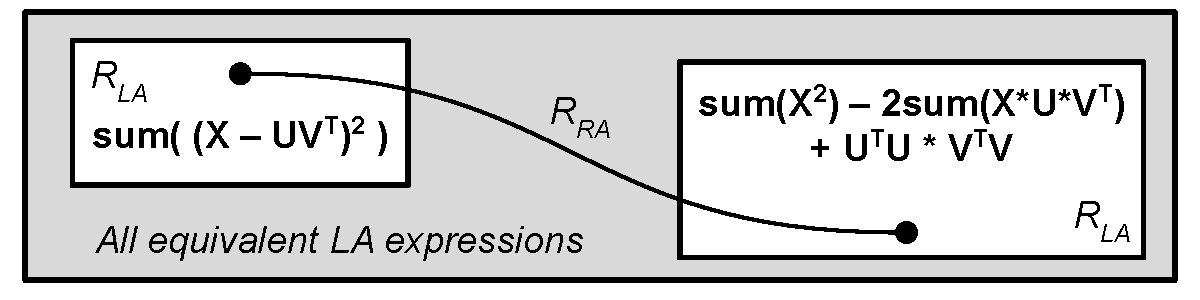
\includegraphics[width=0.8\linewidth]{wormhole}
%     \caption{Venn diagram of LA and/or RA expressions.}
%     \label{wormhole}
% \end{figure}{}

% \begin{figure}
%     \centering
% \begin{tikzcd}
% e_{LA} \arrow[rr, "=" description, no head, dotted] \arrow[d, "R_{LR}"'] &           & e'_{LA} \arrow[d, "R_{LR}"]  \\
% e_{RA} \arrow[r, "R_{EQ}"]                                               & \mathcal{C}(e_{RA}) \equiv \mathcal{C}(e'_{RA})  & e'_{RA} \arrow[l, "R_{EQ}"']
% \end{tikzcd}
    
%     \caption{Two LA expressions $e_{LA}$ and $e'_{LA}$ are equivalent \textit{iff} their
%     relational counterparts $e_{RA}$ and $e'_{RA}$ have isomorphic
%       canonical forms $\mathcal{C}(e_{RA}), \mathcal{C}(e'_{RA})$. $R_{LR}$ translates a LA expression to RA and $R_{EQ}$ are the relational equality rules. }
%     \label{proofsketch}
% \end{figure}{}

% \begin{figure}
%     \centering
%     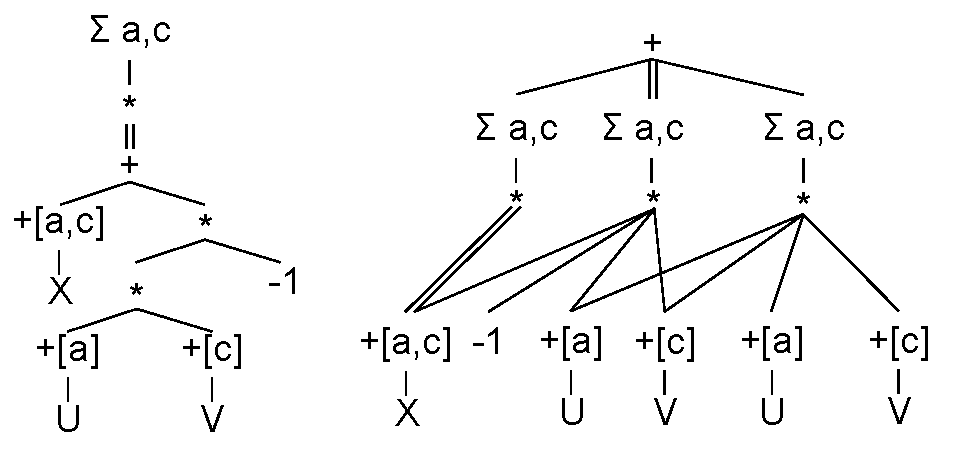
\includegraphics[width=0.9\linewidth]{img/radags.pdf}
%     \caption{RA DAGs for $sum((X-UV^T)^2)$ (left) and its canonical form (right). 
%     % \label{fig:radags}
% \end{figure}{}

% \begin{figure*}
%     \centering 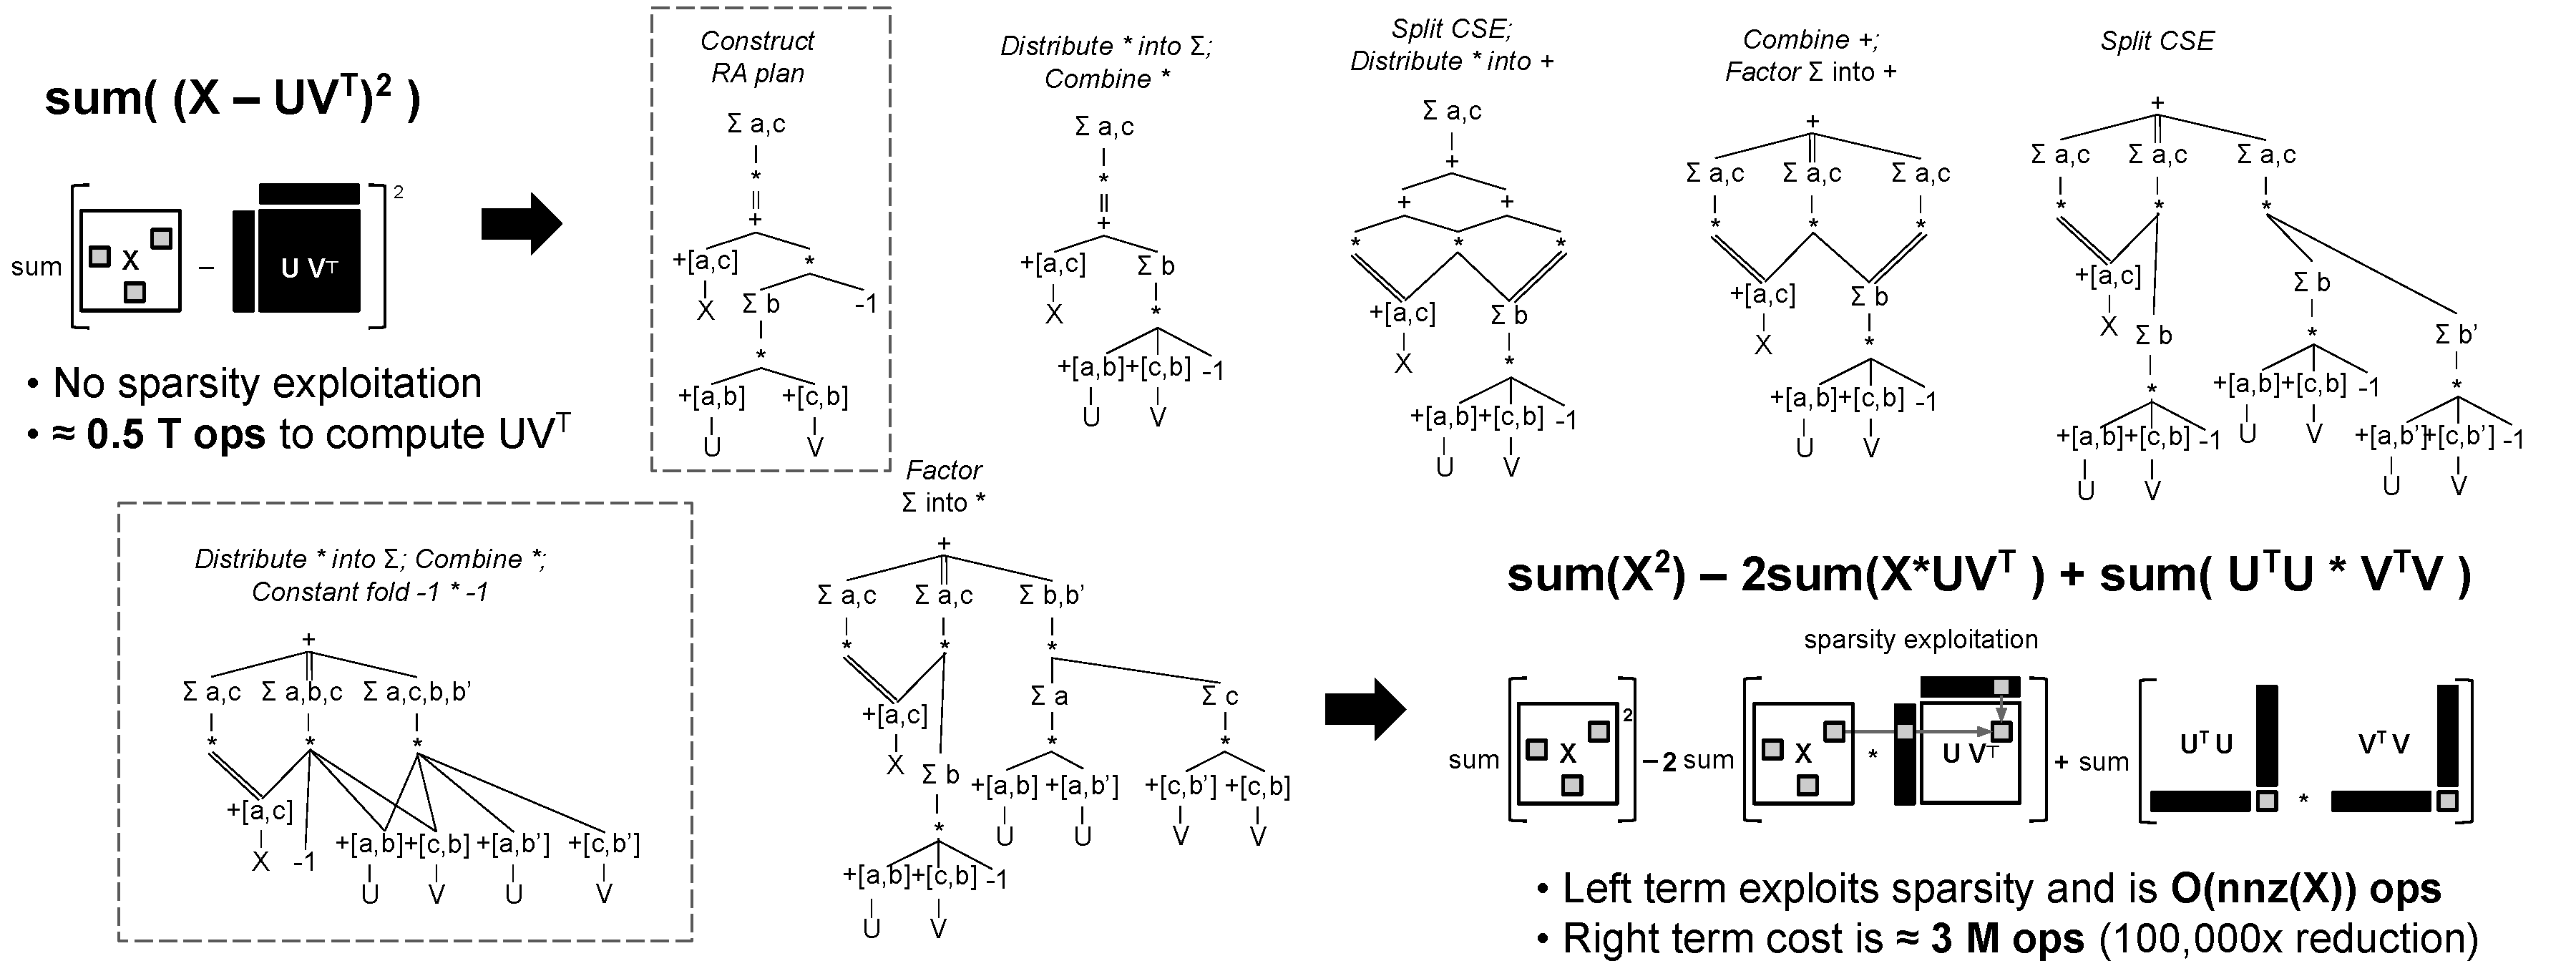
\includegraphics[width=\textwidth]{parrot}
%     \caption{Rewriting details using $R_{LR}$ and $R_{EQ}$ and the
%       optimization's impact on execution cost. Here we show the general case
%       where $U$ and $V$ are matrices, and $X*UV^T$ is computed with a fused
%       chain multiplication operator that exploits sparsity. Dashed lines
%       highlight the initial RPlan and its canonical form. }
%     \label{parrot}
% \end{figure*}




\subsection{Rules \texorpdfstring{$R_{EQ}$}{R\_EQ} : from RA to RA}

The equational rules for RA consists of seven identities shown in
Figure~\ref{RRC}, and denoted by $R_{EQ}$.  The seven rules are
natural relational algebra identities, where $\times$ corresponds to
natural join, $+$ to union (of relations with the same schema) and
$\sum_i$ to group-by and aggregate.  In rule~\ref{RRC_ac},
$i \notin Attr(A)$ means that $i$ is not an attribute of $A$, and
$dim(i)$ is the dimension of index $i$.  For a very simple
illustration of this rule, consider $\sum_i 5$.  Here $5$ is a
constant, i.e. a relation of zero arity, with no attributes.  The rule
rewrites it to $5 dim(i)$, where $dim(i)$ is a number representing the
dimension of $i$.

%%% (Dan: I think the example below is wrong. In RA you must have
%%% indices, can't write $x+1$.
%  $\sum_i (x + 1)$ where $x$ is a vector of length 10 and
% $x + 1$ adds $1$ with each entry of $x$. Following rule~\ref{RRC_ap},
% pushing down the summation rewrites the expression to
% $\sum_i x + \sum_i 1$, and now rule~\ref{RRC_ac} rewrites $\sum_i 1$
% to $|i| * 1 = 10$.


\subsection{\rvo{Completeness of the Optimization Rules}}\label{ranf}

As we have seen at the beginning of this section, when rewriting LA
expressions using identities in linear algebra we may get stuck. Instead, by
rewriting the expressions to RA, the seven identities in $R_{EQ}$ are
much more powerful, and can discover more rewrites.
We prove
here that this approach is {\em complete}, meaning that, if two LA
expressions are semantically equivalent, then their equivalence can be
proven by using rules $R_{EQ}$.  The proof consists of two parts: (1)
the rules $R_{EQ}$ are sufficient to convert any RA expression $e$ to
its {\em normal form} (also called {\em canonical form})
$\mathcal{C}(e)$, and back, (2) two RA expressions $e, e'$ are
semantically equivalent iff they have isomorphic normal forms,
$\mathcal{C}(e) \equiv \mathcal{C}(e')$.
% 
% 
% 
% In general, any equivalent LA expressions can be rewritten to each other using
% our RA representation and equalities. In other words, the relational equalities
% $R_{EQ}$ are \textit{complete} w.r.t. linear algebra semantics. For
% optimization, this means RPlan and its equalities completely represent the
% search space of the optimization problem: we can rewrite an LA expression to any
% of its equals if we first translate it into RA, then apply a chain of equalities
% from $R_{EQ}$, and finally translate the result back to LA. As
% Figure~\ref{wormhole} illustrates, while the usual linear algebra identities
% $R_{LA}$ can only create disjoint equality space for our example expression pre-
% and post-optimization, the relational rules connects the space and rewrite the
% slow expression to the fast one. We sketch a proof of completeness in this
% section.
% 
% Figure~\ref{proofsketch} shows the main steps at a high level: two LA
% expressions are semantically equivalent if and only if their canonical
% form in RA are isomorphic, where $R_{LR}$ translates each expression
% to RA and $R_{EQ}$ takes the RA expression to its canonical form.

% Throughout this section we write $e\ R_{EQ}^*\ e'$ when $e, e'$ can be
% proven equal by using the identities in $R_{EQ}$ (Fig.~\ref{RRC}).

% By semantically equivalent, we
% mean two expressions evaluate to the same result given any same input (variable
% assignment). We define isomorphism of RA canonical forms in Section~\ref{ranf}.
We first give formal definitions for several important constructs. First, we interpret a relation as a function from {\em tuples} to a {\em semiring}. For simplicity we assume all attributes have the same domain $\D$. 
\begin{defn}{{\em (Relations)}}
  Fix a semiring $\SR$.  An {\em $\SR$-\textbf{relation}} is a function $A: \D^a \rightarrow \SR$ where $a$ is the {\em arity} of the relation.
% We write $|\D|$ for the size of domain $\D$. 
\end{defn}
When $\SR=\N$, then an $\N$-relation is a standard relation under bag semantics. When the domain is $\D = [n]$ for some natural number $n$ and $\SR=\R$, then an $\R$-relation is a tensor over the reals.  Next we define expressions over operators from Table~\ref{tPlanOps}. 

\begin{defn}{{\em (Expressions)}}\label{raexpr}
An expression in RA is either \begin{enumerate*}
    \item an \emph{\textbf{atom}} $r$ of the form $R(x_1, ..., x_a)$ where $R$ is a relation name and $(x_1, ..., x_a)$ a tuple of variables and/or constants, or
    \item a {\em natural join} of two expressions $e_1 \times e_2$, or 
    \item a {\em  union} of two expressions, $e_1 + e_2$, or
    \item an {\em aggregate},  $\sum_x e$. 
\end{enumerate*}{}
\end{defn}{}
Because the order of consecutive aggregates does not matter, we write $\sum_{\set{x_1, \dots, x_n}} e$ for $\sum_{x_1} \dots \sum_{x_n} e$. 
Given an expression $e$, we say that a variable $x$ is \emph{\textbf{bound}} in $e$, if $e$ contains an aggregate of the form $\sum_x e'$; 
otherwise it is \emph{\textbf{free}}. We write $vars(e)$ for the set of variables in $e$, $bv(t)$ for the set of bound variables, and $fv(t)$ for the set of free variables.
We interpret every expression $e$ as a lambda expression $\lambda fv(e) . e$ where the parameters $fv(e)$ may follow a given order, e.g. from an unbind operator if $e$ was converted from LA\footnote{A bind operator $[i,j]$ converts a matrix $A$ to an atom $A(i,j)$.}.
 In the body of the lambda expression, any atom $R(x_1, \dots , x_a)$ evaluates to some $s \in \SR$, and $+, \times$ and $\sum$ compute over $\SR$. We say two RA expressions are equivalent iff they evaluate to the same result given any same inputs: 

\begin{defn}{\em (Equivalence of Expressions)} Fix  expressions $e_1, e_2$ over the relation symbols $R_1, \ldots, R_n$.  We say that $e_1, e_2$ are {\em \textbf{equivalent}} over the semiring $\SR$ and the domain $\D$ if they have the same free variables, and for all interpretations $\pmb{I} = (R_1^I, \ldots, R_n^I)$ where $R_j^I : \D^{a_j} \rightarrow \SR$ for $j=1, \ldots, n$ the two expressions return the same answer, $e_1(\pmb{I}) = e_2(\pmb{I})$.  We write $e_1 =_{\SR, \D} e_2$ to mean $e_1$ and $e_2$ are equivalent.  When $e_1 =_{\SR, \D} e_2$ for all domains $\D$, then we abbreviate $e_1 =_\SR e_2$; when this holds for all semirings $\SR$, then we write $e_1 = e_2$.
\end{defn}{}

Now we give names for special forms of expressions at each level of the normal form.
\begin{defn}{{\em (R-monomials, Terms, R-polynomials)}}\label{forms} 
 An \emph{\textbf{R-monomial}}, $m$, is a product of any number of atoms. A \emph{\textbf{term}}, $t$, is a summation expression of the form $\sum_{\pmb{x}} m$, where $\pmb{x}$ is a set of variables and $m$ is an R-monomial.  An \emph{\textbf{R-polynomial}}, $e$, is an expression of the form $c_0 + c_1 t_1 + \dots + c_n t_n$ where $c_0,\ldots,c_n$ are constants in the semiring $\SR$ and $t_1, \ldots, t_n$ are  terms. 
 In summary:
\begin{alignat}{3}
      &m & & := r_1 \times \dots \times r_n && \mbox{R-monomials} \label{eq:r:monomial} \\
      &t & & := \textstyle \sum_{\pmb{x}} m  &&  \mbox{terms} \label{eq:term} \\
      &e & & := c_0 + c_1 t_1 + \dots + c_n t_n \, && \mbox{R-polynomials} \label{eq:r:polynomial}
\end{alignat}{}
We identify the R-monomial $m$ with a bag of atoms denoted by $bag(m) \defeq \set{r_1, \ldots, r_n}$.
\end{defn}{}

\begin{ex}{} An R-polynomial over $\N$-relations is a union of conjunctive queries precisely.  For example, the polynomial $\sum_{j} A(i,j) \times A(i,j) \times B(j,k) \times B(j,k) + \sum_{\ell} A(i,\ell) \times C(\ell,k)$ is precisely the UCQ $Q(i,k) \equiv \exists j (A(i, j) \wedge A(i, j) \wedge B(j, k) \wedge B(j, k)) \vee \exists \ell (A(i, l) \wedge C(l, k))$ under bag semantics.  Notice that
% When the relations are matrices, the polynomial also represents the linear algebra expression $A^2B^2 + AC $, where $A^2$ squares the matrix element-wise. 
  the monomial $A(i,j) \times A(i,j) \times B(j,k) \times B(j,k)$ is the same as $A(i,j) \times B(j,k) \times A(i,j) \times B(j,k)$, and we view it as the bag $\{A(i,j), A(i,j), B(j,k), B(j,k)\}$, and also abbreviate it as $A^2(i,j) \times B^2(j,k)$.
\end{ex}
Before we formally define our canonical form, we need to define two syntactical relationships between our expressions, namely {\em homomorphism} and {\em isomorphism}. Fix terms $t = \sum_{\pmb{x}} m$ and $t' = \sum_{\pmb{x'}} m'$, and let $f: \pmb{x} \rightarrow \pmb{x}'$ be any function. Let $r \in bag(m)$ be an atom of $m$. We write $f(r)$ for the result of applying $f$ to all variables of $r$. We write $f(bag(m))$ for the bag obtained by applying $f$ to each atom $r \in bag(m)$. 
\begin{defn}{\em (Homomorphism)}
  Fix two terms $t, t'$.  A \emph{\textbf{homomorphism}}, $f : t \rightarrow t'$, is a function $f: \pmb{x} \rightarrow \pmb{x}'$ such that $f(bag(m))=bag(m')$.
% Note that $f$ is a one-to-one mapping between $bag(m)$ and $bag(m')$.
\end{defn}{}
\begin{ex}
  Let $t_1 = \sum_{vws} A(i,v) \times B(v,w) \times A(i,s)$ $t_2= \sum_{jk} A^2(i,j) \times B(j,k)$ and $t_3 = \sum_{jk} A(i,j) \times B(j,k)$, and consider the function $f: \set{v,w,s} \rightarrow \set{j,k}$ defined by $v \mapsto j, w \mapsto k, s \mapsto j$.  Then this is a homomorphism $f : t_1 \rightarrow t_2$.  On the other hand $f$ is {\em not} a homomorphism from $t_1 \rightarrow t_3$, because $f(bag(t_1)) = \set{A(i,j), B(j,k), A(i,j)}$ contains the atom $A(i,j)$ twice, while $bag(t_3)$ contains it only once.
\end{ex}
Notice that $t_1, t_2$ must have exactly the same free variables.  By convention, we extend $f$ to be the identity on the free variables.  The following facts are easily verified:
% Otherwise we have $x \in vars(t_2)$ and $x \not\in f(vars(t_1))$, but $f(vars(t_1)) \not = vars(t_2)$. Further, because a homomorphism is a function, it is closed under composition. In summary we have the following facts:
\begin{fact}\label{surjective}
Every homomorphism $f : t_1 \rightarrow t_2$ is a \emph{\textbf{surjective}} function $vars(t_1) \rightarrow vars(t_2)$.
\end{fact}
% \begin{proof}
% Suppose for the sake of contradiction that a homomorphism $f: t_1 \rightarrow t_2$ is not 
% surjective. Then there exists an variable $x \in vars(t_2)$ that is not in $f(vars(t_1))$, 
% and so the atom containing $x$ does not appear in $f(t_1)$. That implies the monomial in $f(t_1)$ cannot be equal to the monomial in $t_2$, so $f$ is not a homomorphism -- contradiction. 
% \end{proof}{}
\begin{fact}\label{compose}
  Homomorphisms are closed under composition.
\end{fact}
% \begin{proof}
% A homomorphism is a function on variables, so composing homomorphisms is just composing functions. 
% \end{proof}{}
A stronger correspondence between terms is an isomorphism:
\begin{defn}[Term Isomorphism]
  Fix two terms $t, t'$.  An \emph{\textbf{isomorphism}} is a homomorphism $f : t \rightarrow t'$ that is a bijection from $vars(t)$ to $vars(t')$.  If an isomorphism exists, then we say that $t, t'$ are \emph{\textbf{isomorphic}} and write $t \equiv t'$.
\end{defn}

\begin{lmm}\label{homocycle}
  Fix two terms $t_1$ and $t_2$.  If there exists hommorphisms $f : t_1 \rightarrow t_2$ and $g: t_2 \rightarrow t_1$ then the terms are isomorphic, $t_1 \equiv t_2$.  More generally, any cycle of homomorphisms $t_1 \rightarrow t_2 \rightarrow t_3 \rightarrow \ldots \rightarrow t_n \rightarrow t_1$ implies that all terms are isomorphic.
\end{lmm}{}
\begin{proof}
  The composition $g \circ f$ is a homomorphism $t_1 \rightarrow t_1$ which, by Fact~\ref{surjective}, is a surjective function $vars(t_1) \rightarrow vars(t_1)$; since $vars(t_1)$ is a finite set, it follows that $g \circ f$ is a bijection, hence so are $f$ and $g$.
%%%% 
%%%% a pair of homomorphisms between two terms are a pair of surjective maps between the terms' variables. A pair of surjective maps induce a bijective map which is an isomorphism.  By Fact~\ref{compose}, if $t_1$ and $t_2$ are on a cycle of homomorphism, we can retract the homomorphism chains between them to obtain a pair of homomorphisms $f: t_1 \rightarrow t_2$ and $g: t_2 \rightarrow t_1$, which implies $t_1 \equiv t_2$.
\end{proof}{}
We are now ready to formally define the canonical form for RA expressions: 

\begin{defn}{\em (Canonical Form)} An RPlan expression (as defined in Table~\ref{tPlanOps}) is {\em \textbf{canonical}} if it is a R-polynomial (Definition~\ref{forms}) containing no isomorphic terms. 
\end{defn}{}

We can canonicalize any expression by pulling $+$ to the top and pushing $\times$ to the bottom, while combining isomorphic terms $c_1 t + c_2 t$ into $(c_1 + c_2) t$: 

\begin{lmm}\label{lCanonPreservesSemantics}
For every RPlan expression there is a canonical expression equivalent to it. 
\end{lmm}{}
\begin{proof}
The proof is a standard application of the rewrite rules $R_{EQ}$ in Figure~\ref{RRC}. 
\end{proof}{}

We can identify canonical expressions syntactically using term isomorphism: 

\begin{defn}{\em (Isomorphic Canonical Expressions)} 
  Fix two R-polynomials $e = c_0 + c_1 t_1 + \dots + c_n t_n$ and $e' = c_0' + c_1' t_1' + \dots + c_m' t_m'$.  We say that $e$ and $e'$ are \emph{\textbf{isomorphic}} if $m=n$, $c_0=c_0'$, and there exists a permutation $\sigma: [n] \rightarrow [n]$ such that $\forall i \in [n]$, $c_i = c_{\sigma(i)}'$, and $t_i \equiv t_{\sigma(i)}'$.
\end{defn}{}

In other words, $e, e'$ are isomorphic if they are essentially the same expression, up to commutativity of $+$ and up to replacing terms $t_i$ with isomorphic terms $t'_{\sigma(i)}$.  In particular,  isomorphic expressions have same free variables.
Our ultimate goal is to identify canonical form isomorphism with equivalence. That is, two canonical expressions are equivalent iff they are isomorphic. For any R-polynomial $e = c_0 + c_1t_1 + \cdots c_nt_n$, we denote by $|vars(e)| \defeq \max_i(|vars(t_i)|)$.  Our main result is the following:

\begin{thm}{(\textbf{Isomorphism Captures Equivalence})}\label{lemma:unique:nf} Let $e_1, e_2$ be two  canonical expressions.  Then the following conditions are equivalent:
  \begin{enumerate}
\itemsep0em
  \item \label{item:1} $e_1 \equiv e_2$ 
  \item \label{item:2} $e_1 = e_2$
  \inlineitem \label{item:3} $e_1 =_\C e_2$
  \inlineitem \label{item:4} $e_1 =_\R e_2$
  \inlineitem \label{item:5} $e_1 =_\N e_2$
  \item \label{item:6} $e_1 =_{\N, \D} e_2$, for some finite domain $\D$ s.t. $|\D| \geq \max(|vars(e_1)|, |vars(e_2)|)$. 
  \end{enumerate}
\end{thm}{}

The implications (\ref{item:1}) $\Rightarrow$ (\ref{item:2}) $\Rightarrow\cdots\Rightarrow$ (\ref{item:6}) are straightforward.  We prove below that (\ref{item:6}) $\Rightarrow$ (\ref{item:1}).  In other words, we prove that, if $e_1, e_2$ are equivalent over the semiring of natural numbers $\N$ and over some domain ``large enough'', then their canonical forms must be isomorpic.  Requiring $|\D|$ to be large enough is necessary, because otherwise two non-isomorphic expressions may be equivalent. For example, if we restrict the relations $X, Y$ to be matrices of dimensions $1 \times 1$, then the expressions $\sum_{i,j} X(i,j) \times Y(i,j)$ and $\sum_{i,j} X(i,j) \times Y(j,i)$ have the same semantics, but different canonical form.  For another example, if $x,y,z$ are vectors of length $2$, these two expressions are equivalent: $\sum_{i,j,k} x(i) \times y(j) \times z(k)+2\sum_i x(i)\times y(i)\times z(i)$ and $\sum_{i,j}x(i)\times y(i)\times z(j)+\sum_{i,j}x(i)\times y(j)\times z(i)+\sum_{i,j}x(j)\times y(i)\times z(i)$, although they are not equivalent when $x,y,z$ are vectors of length $\geq 3$.

\begin{proof} We prove (\ref{item:6}) $\Rightarrow$ (\ref{item:1}).
% $$\forall \D \mbox{ s.t. } |\D|\geq |vars(e_1)| \wedge |\D|\geq |vars(e_2)| : e_1 =_{\N, \D} e_2 \Rightarrow e_1  \equiv e_2 $$
  Assume that $e_1(\pmb{I})=e_2(\pmb{I})$ for all interpretations $\pmb{I}$ over the domain $\D$.  We start by observing that the constant terms in $e_1$ and $e_2$ must be equal, i.e. if $e_1 = c_0 + \ldots, e_2 = c_0' + \ldots$ then $c_0 = c_0'$.  This follows by choosing $\pmb{I}$ to consists of empty relations, in which case $e_1(\pmb{I})=c_0$ and $e_2(\pmb{I})=c_0'$, proving $c_0=c_0'$.  Thus, we can cancel the constant terms and assume w.l.o.g. that $e_1,e_2$ have no constant terms.
Next, we show that we can  assume w.l.o.g. that  $e_1$ and $e_2$ have no free variables.  Otherwise, denote by $\pmb{x}$ the free variables in $e_1$ and $e_2$ (they must be the same in order for $e_1$, $e_2$ to be equivalent), and define $e_1' = \sum_{\pmb{x}} e_2$ and $e_2' = \sum_{\pmb{x}} e_2$.  It is easy to check that $e_1', e_2'$ are also equivalent and, if we prove that they are isomorphic, then so are $e_1, e_2$.  Thus, we will assume w.l.o.g. that $e_1, e_2$ have no free variables.
%
%  where $\pmb{i}$ is the set of free variables of $e_1$ and $e_2$. We can easily show $e_1 = e_2 \Rightarrow e_1' = e_2'$ and $e_1' \equiv e_2' \Rightarrow e_1 \equiv e_2$, and with a proof of $e_1' = e_2' \Rightarrow e_1' \equiv e_2'$ it follows $e_1 = e_2 \Rightarrow e_1 \equiv e_2$. 
% 
% We now prove the right-to-left direction through its contrapositive: 
% 
% $$e_1 \not \equiv e_2 \Rightarrow e_1 \not = e_2$$
% 
Suppose that $e_1$ and $e_2$ contain two terms that are isomorphic: that is, $e_1$ contains $c_it_i$, $e_2$ contains $c_j't_j'$, and $t_i \equiv t_j'$.  In particular, $t_i=t_j'$ i.e. they are also equivalent.  Assuming $c_i \geq c_j'$, we subtract $c_j't_j'$ from both $e_1$ and $e_2$; now $e_1$ contains $(c_i - c_j')t_i$, while $e_2$ no longer contains $t_j'$.  By repeating this process, we remove any pair of isomorphic terms from $e_1, e_2$.  If $e_1, e_2$ were isomorphic, then after this process we remove all terms and both $e_1, e_2$ becomes 0.  Suppose by contradiction that this is not the case, thus $e_1 = c_1 t_1 + c_2 t_2 + \ldots c_m t_m$, $e_2 = c_1' t_1' + \cdots + c_n' t_n'$, and, denoting $T \defeq \set{t_1, \ldots, t_m, t_1', \ldots, t_n'}$ the set of terms in both expressions, no two terms in $T$ are isomorphic.  Assuming $m >0$ or $n > 0$, we prove that $e_1 =_{\N,\D} e_2$ is a contradiction.


Let us denote by $t < t'$ when there exists a homomorphism
$t \rightarrow t'$.  Then $<$ defines a partial order on $T$,
i.e. there is no $<$-cycle, otherwise Lemma~\ref{homocycle} would
imply that some terms are isomorphic.  Let $t_1 \in T$ be any minimal
element under $<$, in other words there is no $t' \in T$ s.t.
$t' < t_1$.  Assume w.l.o.g. that $t_1$ is a term in $e_1$.  We will
construct an instance $\pmb{I}$ that is ``canonical'' for $t_1$, and
prove that $e_1(\pmb{I}) \neq e_2(\pmb{I})$.  Assume
$t_1 = \sum_{\pmb{x}} r_1^{k_1} \times \cdots r_m^{k_m}$, where
$r_1, \ldots, r_k$ are distinct atoms, and
$r_i^{k_i} \defeq r_i \times \cdots \times r_i$ ($k_i$ times).  Let
$n = |\pmb{x}|$, and recall that, by assumption, $|\D| \geq n$.
Choose any injective function $\theta : \pmb{x} \rightarrow \D$; to
reduce clutter we assume w.l.o.g. that $\D = \set{1,2,\ldots, n}$ and
$\theta(x_1) = 1, \ldots, \theta(x_n) = n$.  Let $u_1, \ldots, u_m$ be
$m$ variables over $\N$, one for each distinct atom in $t_1$.  We define
the canonical $\pmb{I}$ as follows.  For each relational symbol $R$,
and for any atom $r_i = R(x_{j_1}, \ldots, x_{j_a})$ that uses the
symbol $R$, we define $R^I(j_1, \ldots, j_a) \defeq u_i$; for all
other tuples in $\D^a$ we define $R(\ldots) = 0$.  This completes the
definition of $\pmb{I}$.  We make two claims.  First,
$t_1(\pmb{I})$ is a multivariate polynomial containing the monomial $c u_1^{k_1} \cdots u_m^{k_m}$. 
% where $c$ is the number of isomorphisms $t \rightarrow t$.
% This claim
% follows immediately from the semantics of $t_1(\pmb{I})$: any function
% $\tau : \pmb{x} \rightarrow \D$ is either an isomorphism
% $t_1 \rightarrow t_1$ (up to the identification of $\D$ with
% $vars(t_1)$), or has a factor that is $=0$.
To see this, write
$t = \sum_{\pmb{y}} r_1' \times \cdots \times r_q'$, and observe that
$t(\pmb{I}) = \sum_{\tau: \pmb{y} \rightarrow \D} \tau(r_1') \times
\cdots \times \tau(r_q')$. When $\tau = \theta$ the R-monomial $\tau(r_1') \times
\cdots \times \tau(r_q') = \theta(r_1') \times
\cdots \times \theta(r_q')$ is precisely $ u_1^{k_1} \cdots u_m^{k_m}$. Second, we claim that,
for any other term $t \in T$, its value $t(\pmb{I})$ on the canonical
instance is some multivariate polynomial in $u_1, \ldots, u_m$ that
does {\em not} contain the monomial $u_1^{k_1} \cdots u_m^{k_m}$.
Indeed, suppose it contained this monomial: then we prove that there
exists a homomorphism $t \rightarrow t_1$, contradicting the
assumption that $t_1$ is minimal.  To see this, consider again $t(\pmb{I}) = \sum_{\tau: \pmb{y} \rightarrow \D} \tau(r_1') \times
\cdots \times \tau(r_q')$.  If this expression includes the monomial
$u_1^{k_1} \cdots u_m^{k_m}$, then for some function
$\tau : \pmb{y} \rightarrow \D$, the bag
$\set{\theta'(r_1'), \ldots, \theta'(r_q')}$ must contain precisely
the atom $\theta(r_1)$ $k_1$-times, the atom $\theta(r_2)$
$k_2$-times, etc.  But that means that $\tau$ is a homomorphism
$t \rightarrow t_1$ (since $\D$ and $vars(t_1)$ are isomorphic via
$\theta$), contradicting our assumption that $t_1$ is minimal.

Thus, we have established that both $e_1(\pmb{I})$ and  $e_2(\pmb{I})$
are multivariate polynomials in $u_1, \ldots, u_m$, but the first
expression contains the monomial  $u_1^{k_1} \cdots u_m^{k_m}$ while
the second does not contain it.  Since $e_1 = e_2$, these two
polynomials must have the same values for all choices of natural
numbers $u_1, \ldots, u_m \in \N$.  It is well known from classical
algebra that, in this case, the two polynomials are identical,
which is a contradiction. 

For a simple illustration, assume $e_1 = t_1$ and $e_2 = t_2$, where
$t_1 = \sum_{x,y,z} R(x,y) \times R(y,z) \times R(z,x)$ and
$t_2 = \sum_{i} R(i,i)^3$.  They are not isomorphic, and our proof
essentially constructs an instance $\pmb{I}$ on which their answers
differ.  Since we have a homomorphism $t_1 \rightarrow t_2$ but not
vice versa, the instance is the canonical instance for $t_1$, i.e.
$R^I(1,2) \defeq u_1$, $R^I(2,3) \defeq u_2$, $R^I(3,1) \defeq u_3$,
and all the other entries are 0.  Then it is easy to verify that
$t_1(\pmb{I})= 3 u_1u_2u_3$ (there are three isomorphisms
$t_1 \rightarrow t_1$), while $t_2(\pmb{I}) = 0$.  Notice that the
canonical instance for $t_2$, $R^I(1,1) \defeq u_1$ and all other
entries are 0, does not make the two expressions different:
$t_1(\pmb{I}) = t_2(\pmb{I}) = u_1^3$.
% 
% 
% 
% 
% 
% 
% We assume w.l.o.g. no term in $e_1$ is isomorphic to any term in $e_2$. 
% Otherwise if $e_1$ contains $c_1t_1$ and $e_2$ contains $c_2t_2$ with $t_1 \equiv t_2$, then we can write $e_1 = c_1 t_1 + e_1'$ and $e_2 = c_2 t_2 + e_2'$ where $e_1'$ and $e_2'$ are polyterms. Assume w.l.o.g that $c_1 \leq c_2$. Since $c_1t_1 + e_1' = c_2 t_2 + e_2'$, $e_1' = (c_2 - c_1)t_2 +e_2'$ and we have removed $t_1$ from $e_1$. 
% Furthermore, $e_1 = e_2 \Rightarrow e_1' = e_2'$ and $e_1' \equiv e_2' \Rightarrow e_1 \equiv e_2$. 
% Then by proving $e_1' = e_2' \Rightarrow  e_1' \equiv e_2'$ we can show the following:
% $$e_1 = e_2 \Rightarrow e_1' = e_2' \Rightarrow  e_1' \equiv e_2' \Rightarrow e_1 \equiv e_2$$
% 
% 
% Each expression can now be viewed as a set of terms, where each term has a constant factor and no two terms are isomorphic. Denoting by $t_1 < t_2$ if there is a homomorphism $t_1 \rightarrow t_2$, we observe homomorphism induces a partial order on the terms of $e_1$ and $e_2$. There is no cycle of homomorphisms, because by Lemma~\ref{homocycle} such a cycle implies isomorphisms, but we have assumed no isomorphic terms. 
% 
% We proceed by constructing a set of witness input relations given which $e_1$ and $e_2$ return different results. First define a bijective function $\phi: \pmb{x} \rightarrow \D$ mapping each variable to a unique value. 
% Define bijective function $\psi(r_n) = v_n$ that maps each atom $r_n = R_n(\pmb{x}_n)$ to a unique natural-valued variable $v_n$, and construct the corresponding input relation $I_n$ such that $I(\phi(\pmb{x}_n)) = v_n$. Finally, set all undefined entries of each input relation to $0$. 
% 
% Given the input relations defined above and some variable assignment $\alpha : \pmb{x} \rightarrow \D$, each atom $R(\pmb{x})$ evaluates to $\psi(R(\phi^{-1}(\alpha(\pmb{x}))))$ which is some $v_n$, if $\alpha(\pmb{x})$ is in the range of $\phi$, and evaluates to $0$ otherwise. Similarly, a R-monomial $m$ evaluates to a monomial over $\N$ on $\alpha$ if $\alpha(x)$ is in the range of $\phi$ for all $x$, and evaluates to $0$ otherwise. In the non-zero case when $m$ evaluates to a monomial $m_v = v_a v_b \dots$, there is a homomorphism $f: m \rightarrow \psi^{-1}(m_v) = \phi^{-1} \circ \alpha$. When $\alpha = \phi$, $f$ is an isomorphism from $m$ to itself. 
% 
% Now let $t_1 = \sum_{\pmb{x}} m_1$ be the minimal term under the partial order induced by homomorphism. Assume w.l.o.g $t_1 \in e_1$. Given the input tensors defined above, $t_1$ evaluates to a polynomial $p_1$. 
% As discussed above every monomial in $p_1$ induces a homomorphism from $m_1$ to some R-monomial over atoms in $m_1$, and one specific monomial $m_{id}$ induces the isomorphism $f_{id}: m_1 \rightarrow m_1$. $m_{id}$ must not appear in any polynomials from other terms in $e_1$ or $e_2$. Otherwise suppose it appears in $t_2$, it would induce a homomorphism $f_2 : m_2 \rightarrow m_1$. 
%  But that is impossible because we have picked $t_1$ to be the minimal term under homomorphism. Therefore, $p_1$ differs from any polynomial from terms in $t_2$. Two polynomials over $\N$ must be isomorphic to be equivalent, therefore $e_1 \not = e_2$. 
% 
\end{proof}{}

We are now ready to establish the completeness of RA equalities, by
showing any equivalent LA expressions can be rewritten to each other
through the translation rules $R_{LR}$ and the canonicalization rules
$R_{EQ}$:

\begin{thm} (\textbf{Completeness of $R_{EQ}$}) Two LA expressions
  are semantically equivalent if and only if their relational form can be rewritten to each other by following $R_{EQ}$. 
\end{thm}
In the following $R_{LR}(e)$ translates LA expression $e$ into RA and $\mathcal{C}(e)$ returns the normal form of $e$. 

\begin{proof}
  Translating $e_1$ and $e_2$ to RA preserves semantics under
  $R_{LR}$. By Lemma~\ref{lCanonPreservesSemantics}, normalizing
  $R_{LR}(e_1)$ and $R_{LR}(e_2)$ preserves semantics. By Theorem~\ref{lemma:unique:nf}, $$R_{LR}(e_1) =_{\R} R_{LR}(e_2) \iff \mathcal{C}(R_{LR}(e_1)) \equiv \mathcal{C}(R_{LR}(e_2))$$ Since every rule in $R_{EQ}$ is reversible, the right-hand-side is true iff $R_{LR}(e_1)$ and $R_{LR}(e_2)$ can be rewritten to each other via $R_{EQ}$. 
\end{proof}

\section{Exploring the Search Space} \label{explore}


With a complete representation of the search space by relational algebra, our
next step is to explore this space and find the optimal expression in it.
Traditional optimizing compilers commonly resort to heuristics to select from
available rewrites to apply. SystemML implements a number of heuristics for its
algebraic rewrite rules, and we discuss a few categories of them here.

\textsc{Competing or Conflicting Rewrites} The same expression may be eligible
for more than one rewrites. For example, $sum(AB)$ rewrites to
$sum(sum_{col}(A)^T*sum_{row}(B))$, but when both $A$ and $B$ are vectors the
expression can also be rewritten to a single dot product. SystemML then
implements heuristics to only perform the first rewrite when the expression is
not a dot product. In the worst case, a set of rules interacting with each other
may create a quadratic number of such conflicts, complicating the codebase.

\textsc{Order of Rewrites} Some rewrite should be applied after others to be
effective. For example, $X/y$ could be rewritten to $X*1/y$ which may be more
efficient, since SystemML provides efficient implementation for sparse
multiplication but not for division. This rewrite should occur before constant
folding; otherwise it may create spurious expressions like $X / (1/y)
\rightarrow X * (1/(1/y))$, and without constant folding the double division
will persist. However, a rewrite like $1/(1 + exp(-X)) \rightarrow sigmoid(X)$
should come after constant folding, in order to cover expressions like $(3-2)/(1
+ exp(-X))$. Since SystemML requires all rewrites to happen in one phase and
constant folding another, it has to leave out\footnote{Another reason to leave
  out this rewrite is that $X*1/y$ rounds twice, whereas $X/y$ only rounds
  once.} rewrites like $X/y \rightarrow X*1/y$.

\textsc{Dependency on Input/Program Properties} Our example optimization from 
$sum((X-UV^T)^2)$  to $sum(X^2) -2U^TXV + U^TU*V^TV$
improves performance only if $X$ is sparse. Otherwise,
computing $X^2$ and $X*UV^T$ would both create dense intermediates. Similarly,
some rewrites depend on program properties like common subexpressions. Usually,
these rewrites only apply when the matched expression shares no CSE with others
in order to leverage common subexpression elimination. Testing input and program
properties like this becomes boilerplate code, making implementation tedious and
adds burden to maintenance.

\textsc{Composing Rewrites} Even more relevant to us is the problem of composing
larger rewrites out of smaller ones. Our equality rules $R_{EQ}$ are very
fine-grained, and any rule is unlikely to improve performance on its own. 
Our example optimization from $sum((X-UV^T)^2)$ to $sum(X^2) - 2U^TXV + U^TU * V^TV$ 
takes around 10 applications of $R_{EQ}$ rules. 
 If an optimizer applies rewrites one by one, it is
then very difficult, if not impossible, for it to discover the correct sequence
of rewrites that compose together and lead to the best performance.

Stepping back, the challenge of orchestrating rewrites is known as the
\emph{phase-ordering problem} in compiler optimization. Tate
et al. \cite{DBLP:journals/corr/abs-1012-1802} proposed a solution  dubbed
\textit{equality saturation} which we adapt and extend in SPORES.

\subsection{Equality Saturation}

Equality saturation optimizes an expression in two steps:

\textit{Saturation}: given the input expression, the optimizer  enumerates
equivalent expressions and collects them into a compact representation called
the E-Graph \cite{10.5555/909447}.

\textit{Extraction}: given a cost function, the optimizer selects the optimal
expression from the E-Graph. An expression is represented by a subgraph of the
E-Graph, and the optimizer uses a constraint solver to find the subgraph
equivalent to the input that is optimal according to the cost function.

\subsubsection*{The E-Graph Data Structure}

\begin{figure}
\centering
    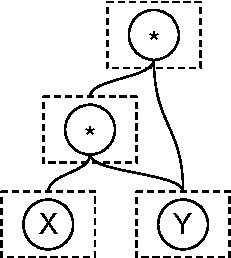
\includegraphics[scale=0.5]{XYY} \qquad 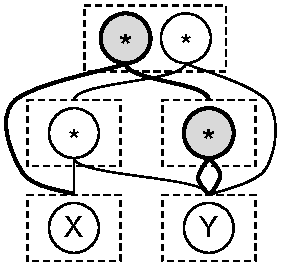
\includegraphics[scale=0.5]{assoc} \qquad 
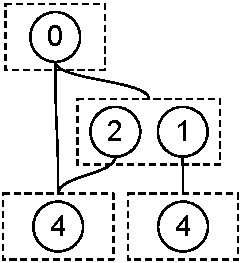
\includegraphics[scale=0.5]{CSE} 
    \vspace{7pt}
    \caption{Left: E-Graph representing $(X \times Y) \times Y$, and the graph after applying
      associativity to the root (middle). New nodes are in gray. Each dashed box is an E-Class.
      Right: the CSE problem. Each node shows its cost.}
    \label{assoc}
    \vspace{10pt}
\end{figure}

An E-Graph represents sets of equivalent expressions. A node in the graph is
called an E-Class, which contains the root operators of a set of equivalent
expressions. The edges are similar to the edges in an abstract syntax tree; but
instead of pointing from an operator directly to a child, each edge points from
an operator to an E-Class of expressions. For example, in Figure~\ref{assoc} the
top class in the middle represents the set of equivalent expressions \{$(X\times Y)\times Y,
X\times (Y\times Y)$\}. Note that the class represents two expressions, each with 2
appearances of $Y$ and one appearance of $X$, whereas each variable only appears
once in the E-Graph. This is because the E-Graph makes sure its expressions share
all possible common subexpressions. As the size of the graph grows, this
compression becomes more and more notable; in some cases a graph can 
represent a number of expressions exponential to its
size \cite{DBLP:journals/corr/abs-1012-1802}. We take advantage of this
compression in SPORES to efficiently cover vast portions of the search
space. If saturation, as described below, carries out to convergence, the E-Graph represents the search space exhaustively. 

An E-Graph can also be seen as an AND-OR DAG over expressions. Each E-Class is an OR node whose children are equivalent expressions from
which the optimizer chooses from. Each operator is an AND node whose children must all be picked if the operator itself is picked. In this dissertation we favor the terms E-Graph and E-Class to emphasize each OR node is an equivalence class. 

\subsubsection*{Saturating the E-Graph}
At the beginning of the optimization process, the optimizer instantiates the
graph by inserting the nodes in the syntax tree of the input expression one by
one in post order. For example, for input $(X\times Y)\times Y$, we construct the left graph
in Figure~\ref{assoc} bottom-up. By inserting in post order, we readily exploit
existing common subexpressions in the input. Once the entire input expression is
inserted, the optimizer starts to extend the graph with new expressions equivalent to
the input. It considers a list of equations, and matches either side of the
equation to subgraphs of the E-Graph. If an equation matches, the optimizer then
inserts the expression on the other side of the equation to the graph. For
example, applying the associativity rule extends the left graph in
Figure~\ref{assoc} with $X\times (Y\times Y)$, resulting in the right graph.
Figure~\ref{eqsat} shows the pseudo code for this process. While inserting new
expressions, the optimizer checks if any subexpression of the new expression is
already in the graph. If so, it reuses the existing node, thereby exploiting all
possible common-subexpressions to keep the E-Graph compact. In
Figure~\ref{assoc}, only two $\times$ are added since the variables $X$ and $Y$ are
already in the graph. Once the entire new expression has been added, the
optimizer then merges the newly created E-Class at its root with the E-Class
containing the matched expression, asserting them equal. Importantly, the
optimizer also propagates the congruent closure of this new equality. For
example, when $A+A$ is merged with $2\times A$, the optimizer also merges $(A+A)^2$
with $(2\times A)^2$. Figure~\ref{eqsat} shows the pseudo code for adding an
expression to E-Graph. This process of match-and-insert is repeated until the
graph stops changing, or reaching a user-specified bound on the number of 
saturation iterations. If this process does converge, that means no rule can add new
expressions to the graph any more. If the set of rules are complete, as is our
$R_{EQ}$, convergence of saturation implies the resulting E-Graph represents
the transitive closure of the equality rules applied to the initial expression.
In other words, it contains \textit{all} expressions equivalent to the input under the equality rules.

\begin{figure}
\begin{lstlisting}[language=Python]
def saturate(egraph, equations):
  for eq in equations: 
    matches = egraph.match(eq.lhs)
    for eclass in matches: 
      ec = egraph.add(eq.rhs)
      egraph.merge(eclass, c)

def add(expr):
  ID = egraph.find(expr)
  if ID != NULL:
    return ID
  else:
    cids = expr.children.map(add)
    ID = egraph.insert(expr.op, cids)
    return ID
\end{lstlisting}
    \caption{Equality saturation pseudocode. 
      % \texttt{match} returns the IDs of the root class of any matching subgraph;
      % \texttt{merge} combines two E-Classes given their IDs; it also propagates
      % the congruent closure of the new equality.
      % Figure~\ref{fig:egraphadd} defines \texttt{add}.
}
    \label{eqsat}
    \vspace{7pt}
\end{figure}
% \begin{figure}
% \begin{lstlisting}[language=Python]
% def add(expr):
%   ID = egraph.find(expr)
%   if ID != NULL:
%     return ID
%   else:
%     cids = expr.children.map(add)
%     ID = egraph.insert(expr.op, cids)
%     return ID
% \end{lstlisting}
%     \caption{Pseudo code for adding an expression to the E-Graph. 
%      % \texttt{find}
%      %  looks for the given expression in the E-Graph, and returns its root ID if
%      %  it already exists, or \texttt{NULL} otherwise. \texttt{insert} adds the
%      %  given operator to the E-Graph, and points its children to E-Classes with the
%      %  given class IDs. 
% }
%     \label{fig:egraphadd}
% \end{figure}

The outer loop that matches equations to the graph can be implemented by a more
efficient algorithm like the Rete algorithm \cite{DBLP:journals/ai/Forgy82} when
the number of equations is large. However, we did not find matching to be
expensive and simply match by traversing the graph. Our implementation uses the
E-Graph data structure from the \texttt{egg}~\cite{willsey2020egg} library. 
\subsubsection*{Dealing with Expansive Rules}
While in theory equality saturation will converge with well-constructed rewrite
rules, in practice the E-Graph may explode for certain inputs under certain rules. For example, a long
chain of multiplication can be rewritten to an exponential number of
permutations under associativity and commutativity (AC rules). If we 
apply AC rules everywhere applicable in each iteration, the graph would soon use
up available memory. We call this application strategy the \emph{depth-first}
strategy because it eagerly applies expansive rules like AC. 
AC rules by themselves rarely affect performance \rvb{\cite{DBLP:conf/edbt/KernertKL15}}, and
SystemML also provides the fused \texttt{mmchain} operator that efficiently computes
multiplication chains, so permuting a chain is likely futile. In practice, AC
rules are useful because they can enable other rewrites. Suppose we have a rule
$R_{factor}: A\times X + B\times X \rightarrow (A+B)\times X$ and an expression $U\times Y + Y\times V$.
Applying commutativity to $Y\times V$ would then transform the expression to be
eligible for $R_{factor}$. With this insight, we change each saturation
iteration to sample a limited number of matches to apply per rule, instead of
applying all matches. This amounts to adding \texttt{matches = sample(matches, limit)} between line 3 and line 4 in Figure~\ref{eqsat}. 
Sampling encourages each rule to be considered equally often
and prevents any single rule from exploding the graph. This helps ensure good
exploration of the search space when exhaustive search is impractical. 
But when it is
possible for saturation to converge and be exhaustive, it still converges with high probability
when we sample matches. Our experiments in Section~\ref{overhead} show sampling
always preserve convergence in practice.

\subsubsection*{Extracting the Optimal Plan}
\label{extraction}

A greedy strategy to extract the best plan from the saturated E-Graph is to
traverse the graph bottom-up, picking the best plan at each level. This assumes
the best plan for any expression also contains the best plan for any of its
subexpressions. However, the presence of common subexpressions breaks this
assumption. In the right-most graph in Figure~\ref{assoc} each operator 
node is annotated with its cost. 
Between the nodes with costs 1 and 2, a greedy strategy would choose 1, which
incurs total cost of $1+4=5$. The greedy strategy then needs to pick the root
node with cost 0 and the other node with cost 4, incurring a total cost of 9. 
However, the optimal strategy is to pick the nodes with 0, 2 and share the same
node with cost 4, incurring a total cost of 6. 

We handle the complexity of the search problem with a constraint
solver. We assign a variable to each operator and each E-Class, then construct
constraints over the variables for the solver to select operators that make up a
valid expression. The solver will then optimize a cost function defined over the
variables; the solution then corresponds to the optimal expression equivalent to
the input. \rvo{We implement both the greedy strategy and the solver-based strategy and compare them
in Section~\ref{overhead}.} 

\subsubsection*{Constraint Solving and Cost Function}
We encode the problem of extracting the cheapest plan from the E-Graph with
integer linear programming (ILP). Figure~\ref{ilp} shows this encoding. For each
operator in the graph, we generate a boolean variable $B_{op}$; for each E-Class
we generate a variable $B_c$. For the root class, we use the variable $B_r$.
Constraint $F(op)$ states that if the solver selects an operator, it must also
select all its children; constraint $G(c)$ states that if the solver selects an
E-Class, it must select at least one of its members. Finally, we assert $B_r$ must 
be selected, which constrains the extracted expression
to be in the same E-Class as the unoptimized expression. These three constraints together
ensure the
selected nodes form a valid expression equivalent to the unoptimized input.
Satisfying these constraints, the solver now minimizes the cost function given
by the total cost of the selected operators. Because each $B_{op}$ represents an
operator node in the E-Graph which can be shared by multiple parents, this
encoding only assigns the cost once for every shared common subexpression. In
our implementation, we use Gurobi~\cite{gurobi} to solve the ILP problem.

\begin{figure}
{\small
    \begin{align*}
Constraints &\equiv B_r \wedge \bigwedge_{op} F(op) \wedge \bigwedge_c G(c)
\\ F(op) &\equiv B_{op} \rightarrow \bigwedge_{c \in op.children} B_c \\ G(c)
&\equiv B_c \rightarrow \bigvee_{op \in c.nodes} B_{op}
\end{align*}
\[\textbf{minimize} \sum_{op} B_{op} \cdot C_{op} \textbf{ s.t. } Constraints\]
    \caption{ILP constraint and objective for extraction. }
    \vspace{-10pt}
    \label{ilp}
}%
\end{figure}
\begin{figure}
\begin{align*}
    \textbf{S}[X\times Y] &= min(\textbf{S}[X], \textbf{S}[Y]) \\ \textbf{S}[X+Y] &=
    min(1, \textbf{S}[X]+\textbf{S}[Y]) \\ \textbf{S}[\sum_i X] &= min(1, |i|
    \cdot \textbf{S}[X])
\end{align*}
    \caption[Sparsity estimation]{Sparsity estimation. We define $sparsity = nnz
      / size$, i.e. a 0 matrix has sparsity $0.0$\protect\footnotemark. $|i|$ is
      the size of the aggregated dimension. }
    \label{fig:cost}
\end{figure}
\footnotetext{Some may find this definition counter-intuitive; we define it so
  to be consistent with SystemML.}

Each operation usually has cost proportional to the output size in terms of
memory allocation and computation. Since the size of a matrix is proportional to
its the number of non-zeroes (nnz), we use SystemML's estimate of nnz as the
cost for each operation. Under our relational interpretation, this corresponds
to the cardinality of relational queries. We use the simple estimation scheme in
Figure~\ref{fig:cost}, which we find to work well. \rvb{We rely on SystemML's 
estimation for non-sum-product operators.} Future work can hinge on the
vast literature on sparsity and cardinality estimation to improve the cost
model.

\subsection{Schema and Sparsity as Class Invariant}
In the rules $R_{EQ}$ used by the saturation process, Rule~(\ref{RRC_ma}) If $i
\not\in A$, $A \times \sum_i B = \sum_i (A \times B)$ contains a condition on attribute
$i$ which may be deeply nested in the expression. This means the optimizer
cannot find a match with a simple pattern match. Fortunately, all expressions in
the same class must contain the same set of free attributes (attributes not
bound by aggregates). In other words, the set of free variables is invariant
under equality. This corresponds precisely to the schema of a database -
equivalent queries must share the same schema. We therefore annotate each class
with its schema, and also enable each equation to match on the schema.

In general, we find class invariants to be a powerful construct for programming
with E-Graphs. For each class we track as class invariant if there is a constant
scalar in the class. As soon as all the children of an operator are found to
contain constants, we can fold the operator with the constant it computes. This
seamlessly integrates constant folding with the rest of the rewrites. We also
treat sparsity as a class invariant and track it throughout equality saturation.
Because our sparsity estimation is conservative, equal expressions that use
different operators may have different estimates. But as soon as we identify
them as equal, we can merge their sparsity estimates by picking the tighter one,
thereby improving our cost function. Finally, we also take advantage of the
schema invariant during constraint generation. Because we are only interested in
RA expressions that can be translated to LA, we only generate symbolic variables
for classes that have no more than two attributes in their schema. This prunes
away a large number of invalid candidates and helps the solver avoid wasting
time on them. We implement class invariants using \texttt{egg}'s Metadata API.

\subsection{Translation, Fusion and Custom Functions}
\label{udfs}
Since equality saturation can rewrite any expression given a set of equations,
we can directly perform the translation between LA and RA within saturation,
simply by adding the translation rules $R_{LR}$ from Figure~\ref{RMR}.
Furthermore, saturation has flexible support for custom functions. The simplest
option is to treat a custom functions as a black box, so saturation can still
optimize below and above them. With a little more effort, we have the option to
extend our equations $R_{EQ}$ to reason about custom functions, removing the
optimization barrier. We take this option for common operators that are not part
of the core RA semantics, e.g. square, minus and divide. In the best scenario,
if the custom function can be modeled by a combination of basic operators, we
can add a rule equating the two, and retain both versions in the same graph for
consideration. In fact, this last option enables us to encode fused operators
and seamlessly integrate fusion with other rewrite rules. As a result, the
compiler no longer need to struggle with ordering fusion and rewrites, because
saturation simultaneously considers all possible ordering. 
\rvo{We note that although supporting custom functions require additional rules in
\sys, these rules are all identities, and they are much simpler than the heuristics
rules in SystemML which need to specify when to fire a rule and how each rule
interacts with another.} \rvt{Finally, although 
SystemML does not directly expose ``physical'' operators, e.g. different matrix
multiplication algorithms, \sys\ readily supports optimization of physical plans. 
For example, we could use two distinct operators for two matrix multiplication 
algorithms, and both would always appear in the same E-Class. Both operators
would share the same child E-Classes, therefore the additional operator only
adds one node for every class that contains a matrix multiply.}

\subsection{Saturation v.s. Heuristics}

Using equality saturation, SPORES elegantly remedies the drawbacks of
heuristics mentioned in the beginning of section~\ref{explore}. First, when two
or more conflicting rewrites apply, they would be added to the same E-Class, and
the extraction step will pick the more effective one based on the global cost
estimate. Second, there is no need to carefully order rewrites, because
saturation simultaneously considers all possible orders. For example, when rules
$R_1$ and $R_2$ can rewrite expression $e$ to either $R_1(R_2(e))$ or
$R_2(R_1(e))$, one iteration of saturation would add $R_1(e)$ and $R_2(e)$ to
the graph, and another iteration would add both $R_1(R_2(e))$ and $R_2(R_1(e))$
to the same E-Class. Third, rules do not need to reason about their dependency on
input or program properties, because extraction uses a global cost model that
holistically incorporates factors like input sparsity and common subexpressions.
Finally, every rule application in saturation applies one step of rewrite on top
of those already applied, naturally composing complex rewrites out of simple
ones.

\subsection{Integration within SystemML}

We integrate SPORES into SystemML to leverage its compiler
infrastructure. \sys\ plugs into the algebraic rewrite pass in SystemML; it
takes in a DAG of linear algebra operations, and outputs the optimized DAG.
Within \sys, it first translates the LA DAG into relational algebra,
performs equality saturation, and finally translates the optimal expression back
into LA. We obtain matrix characteristics such as dimensions and sparsity
estimation from SystemML. Since we did not focus our efforts in supporting
various operators and data types unrelated to linear algebra computation (e.g.
string manipulation), we only invoke SPORES on important LA expressions
from the inner loops of the input program.

% \begin{figure}
%     \centering 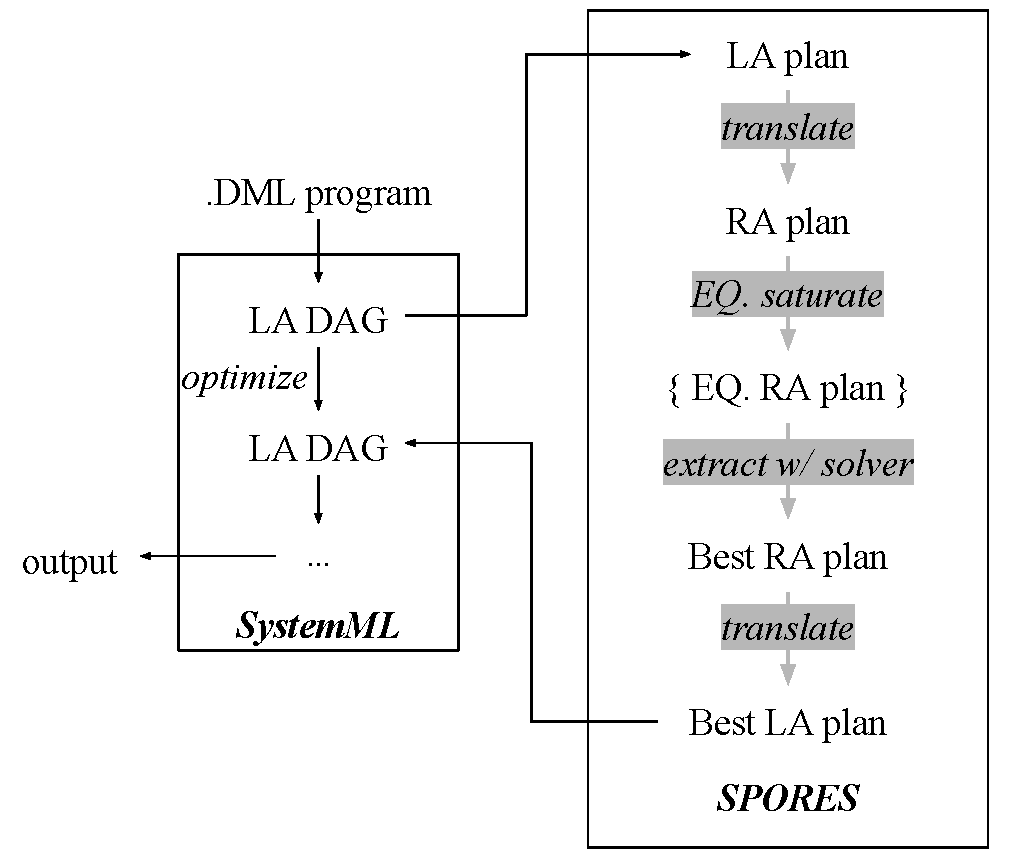
\includegraphics[width=0.6\linewidth]{arch}
%     \caption{Architecture of SPORES \& integration in SystemML}
%     \label{warp}
% \end{figure}{}

\section{Evaluation} \label{sec:evaluation}

We evaluate SPORES to answer three research questions about our
approach of relational equality saturation: 
\begin{itemize}
    \item \textbf{Section~\ref{relcomp}}: can SPORES derive hand-coded
      rewrite rules for sum-product optimization?
    \item \textbf{Section~\ref{perf}}: can SPORES find optimizations that
      lead to greater performance improvement than hand-coded rewrites and
      heuristics? 
      \item \textbf{Section~\ref{overhead}}: does SPORES induce compilation overhead afforded by its performance gain?  
\end{itemize}

We ran experiments on a single node with Intel E74890 v2 @ 2.80GHz with hyper-threading, 
1008 GB RAM, 1 Nvidia P100 GPU, 8TB
disk, and Ubuntu 16.04.6. We used OpenJDK 1.8.0, Apache Hadoop 2.7.3, and Apache
Spark 2.4.4. Spark was configured to run locally with 6 executors, 8
cores/executor, 50GB driver memory, and 100GB executor memory. Our baselines are
from Apache SystemML 1.2.0 and TensorFlow r2.1. We compile all TensorFlow functions
with XLA through \verb|tf.function|, and enable GPU.  

\subsection{Completeness of Relational Rules} \label{relcomp}
% \begin{figure}
% \begin{enumerate}
%   \item $sum(A+B) = sum(A)+sum(B)$
%   \item $sum(X^T) = sum(X)$
%   \item $sum(sum_{row}(X)) = sum(X)$,  $sum_{col}$ similar
%   \item $(UV)^T = V^TU^T$, $(U*V)^T=U^T*V^T$
%   \item $(A+B)^T=A^T + B^T$, $(X^T)^T=X$
%   \item $(X*Y)*Z = X*(Y*Z)$, $X*Y = Y*X$
%   \item $A * X + b * X =  (A+b)*X$
%   \item $a * UV = (a*U) V$
% \end{enumerate}
% \caption{LA equality rules $R_{LA}$ for comparison. \textcolor{red}{TODO fix caption}}
% \label{RLA}
% \end{figure}

% \begin{figure*}
%     \centering
%     \begin{tabular}{|l|c|l|}
%     \hline
%      Method Name & \# & Example Rewrite \\
%      \hline
     
% \verb|UnnecessaryOuterProduct| & 3 & \verb|X*(Y%*%1) ->| \verb| X*Y, if Y col vector |\\

% \verb|ColwiseAgg| & 3 & \verb|colsums(X) -> sum(X) or X, if col/row vector |\\

% \verb|RowwiseAgg| & 3 & \verb|rowsums(X) -> sum(X) or X, if row/col vector |\\

% \verb|ColSumsMVMult| & 1 & \verb|colSums(X*Y) -> t(Y) %*% X, if Y col vector |\\

% \verb|RowSumsMVMult| & 1 & \verb|rowSums(X*Y) -> X %*% t(Y), if Y row vector |\\

% \verb|UnnecessaryAggregate| & 9 & \verb|sum(X) -> as.scalar(X), if 1x1 dims |\\
% \verb|EmptyAgg| & 3 & \verb|sum(X) -> 0, if nnz(X)==0 |\\
% \verb|EmptyReorgOp| & 5 & \verb|t(X) -> matrix(0, ncol(X), nrow(X)) if nnz(X)==0|\\
% \verb|EmptyMMult| & 1 & \verb|X%*%Y -> matrix(0,...), if nnz(Y)==0|\\
% \verb|IdentityRepMatrixMult| & 1 & \verb|X%*%y -> X if y matrix(1,1,1) |\\
% \verb|ScalarMatrixMult| & 2 & \verb|X%*%y -> X*as.scalar(y), if y is a 1-1 matrix |\\
% \verb|pushdownSumOnAdd| & 2 & \verb|sum(A+B) -> sum(A)+sum(B) if dims(A)==dims(B) |\\

% \verb|DotProductSum| & 2 & \verb|sum(v^2) -> t(v)%*%v if ncol(v)==1 |\\
% \verb|reorderMinusMatrixMult| & 2 & \verb|(-t(X))%*%y -> -(t(X)%*%y) |\\

% \verb|SumMatrixMult| & 3 & \verb|sum(A%*%B) -> sum(t(colSums(A))*rowSums(B)) if not dot product|\\
% \verb|EmptyBinaryOperation| & 3 & \verb|X*Y -> matrix(0,nrow(X), ncol(X)) / X+Y->X / X-Y -> X |\\
% \verb|ScalarMVBinaryOperation| & 1 & \verb|X*y -> X*as.scalar(y), if y is a 1-1 matrix |\\
% \verb|UnnecessaryBinaryOperation| & 6 & \verb|X*1 -> X (dep: should come after rm unnecessary vectorize) |\\
% \verb|BinaryToUnaryOperation| & 3 & \verb|X*X -> X^2, X+X -> X*2, (X>0)-(X<0) -> sign(X) |\\
% \verb|MatrixMultScalarAdd| & 2 & \verb|eps+U%*%t(V) -> U%*%t(V)+eps, U%*%t(V)-eps -> U%*%t(V)+(-eps) |\\
% \verb|DistributiveBinaryOperation| & 4 & \verb|(X-Y*X) -> (1-Y)*X |\\
% \verb|BushyBinaryOperation| & 3 & \verb|(X*(Y*(Z%*%v))) -> (X*Y)*(Z%*%v) |\\
% \verb|UnaryAggReorgOperation| & 3 & \verb|sum(t(X)) -> sum(X) |\\
% \verb|UnnecessaryAggregates| & 8 & \verb|sum(rowSums(X)) -> sum(X) |\\
% \verb|BinaryMatrixScalarOperation| & 3 & \verb|as.scalar(X*s) -> as.scalar(X)*s |\\

% \verb|pushdownUnaryAggTransposeOperation| & 2 & \verb|colSums(t(X)) -> t(rowSums(X)) |\\
% \verb|pushdownCSETransposeScalarOperation| & 1 & \verb|a=t(X), b=t(X^2) -> a=t(X), b=t(X)^2 for CSE t(X) |\\

% \verb|pushdownSumBinaryMult| & 2 & \verb|sum(lamda*X) -> lamda*sum(X) if lamdba is scalar|\\
% \verb|UnnecessaryReorgOperation| & 2 & \verb|t(t(X))->X potentially introduced by other rewrites |\\
% \verb|TransposeAggBinBinaryChains| & 2 & \verb|t(t(A)%*%t(B)+C) -> B%*%A+t(C) |\\
% \verb|UnnecessaryMinus| & 1 & \verb|-(-X)->X potentially introduced by other rewrites |\\
% \hline
% \end{tabular}{}
%     \caption{Sum-product rewrites in SystemML. The first column lists the name for each rewrite method. Each 
%     method implements a number of rewrite patterns, and the second column shows how many. The last column shows an example rewrite for each method. Following SystemML's notation, scalars are in lower-case and matrices/vectors in upper-case. \texttt{\%*\%} is matrix multiply,  \texttt{t()} is transpose, and \texttt{nnz(X)} is the number of non-zeroes in $X$. 
%     Equality saturation derives rewrites form all 31 methods (84 patterns) with relational  rules. }
%     \label{rewritecomplete}
% \end{figure*}{}

Theoretically, our first hypothesis is validated by the fact that our relational
equality rules are complete w.r.t. linear algebra semantics. To test completeness in
practice\footnote{\textit{``I have only proved it correct, not tried it''} --
  Donald Knuth}, our first set of experiments check if SPORES
can derive the hand-coded sum product rewrite rules in SystemML. To do this, we
input the left hand side of each rule into SPORES, perform equality
saturation, then check if the rule's right hand side is present in the saturated
graph. The optimizer is able to derive
all 84 sum-product rewrite rules in SystemML using relational equality rules. 
Refer to the long version of this chapter \cite{SPORESarxiv} for a list of these rewrites. 
We believe replacing the 84 ad-hoc
rules with our translation rules $R_{LR}$ and equality rules $R_{EQ}$ would greatly
simplify SystemML's codebase. Together with equality saturation, our relational
rules can also lead to better performance, as we demonstrate in the next set of
 experiments.

% We then replace the RA equalities with the usual
% linear algebra equalities listed in Figure~\ref{RLA} and perform the same test.
% This time, the optimizer can only derive 33 out of 59 rules.
% TODO get number

% While we argue the experiment shows the benefit of RA rules over LA rules, one
% may wonder if we over-constrain the LA rules; perhaps 
% by adding a few additional rules, the LA rules can become complete as well. To
% this we answer that our RA rules can be viewed as an enhanced version of LA
% rules. While there may be other alternatives, we have shown our rules to be apt
% both in theory and in practice. From a different angle, the rules in
% Figure~\ref{rewritecomplete} from SystemML can also be regarded as an enhanced
% version of LA equalities. However, it is incomplete because it cannot derive 
% our example optimization of $sum((X-UV^T)^2)$. Practically, our RA rules are both more
% principled and simpler than the hand-coded rules, so adopting the former can
% simplify the codebase and alleviate maintenance burden. Together with equality saturation, our RA
% rules can also lead to better performance, as we demonstrate in the next set of
% experiments.

% TODO runtime evaluation 
\subsection{Run Time Measurement} \label{perf}
We compare SPORES against SystemML's native optimizations for their
performance impact. As baseline, we run SystemML with optimization level 2 (\texttt{opt2}),
which is its default and includes all advanced rewrites like constant folding
and common subexpression elimination. We additionally enable SystemML's native
sum-product rewrites and operator fusion. \rvo{When using SPORES, we disable SystemML's
native sum-product rewrites, which means disabling the 84 rules discussed in Section~\ref{relcomp}.
We compile and execute 5 real-world
algorithms including Generalized Linear Model (GLM), Multinomial
 Logistic Regression (MLR), Support Vector Machine (SVM), Poisson
 Nonnegative Matrix Factorization (PNMF), and Alternating Least Square
 Factorization (ALS). We configure GLM and MLR to learn a probit model as a binary classifier.
 We take the implementation of these algorithms from
 SystemML's performance benchmark suite \cite{smlperftest}. All algorithms were used as benchmarks in previous
 optimization research \cite{ElgamalLBETRS17} \cite{DBLP:journals/pvldb/BoehmRHSEP18}.
We use the same input datasets from
\cite{DBLP:journals/pvldb/BoehmRHSEP18}, specifically the Amazon books review dataset
(Amazon/A) \cite{DBLP:conf/www/HeM16}, the Airline on-time performance dataset (Flights/F) \cite{flights},
the Netflix movie rating dataset (Netflix/N) \cite{netflix}, and the MNIST8M dataset (MNIST/M) \cite{mnist}.
In order to fit the computation in memory, we down sample each dataset to obtain inputs of small, medium and large sizes.
For the Amazon and Netflix data, AS/NS contian 25k reviews, AM/NM 50k, and AL/NL 100k. We convert the data
to a review matrix, where columns are items and rows are customers, then use it as input to ALS and PNMF. 
For the Flights and MNIST
datasets, FS/MS contain 2.5M rows, FM/MM 5M, and FL/ML 10M. We use these datasets as input to GLM / MLR / SVM.
Each algorithm learns if a flight is delayed more than 5 hours, or if an image shows the digit 2. In TensorFlow experiments we generate random inputs
that match the size of the intermediate data in the corresponding benchmark.}  
\rvt{
Our approach focuses on optimizing sum-product operations with the assumption that these operations take up the
majority of run time in machine learning programs. We test this assumption by profiling our benchmark programs
on the largest version of each dataset. Figure~\ref{heavy} shows that for each program on each input dataset,
sum-product operations including matrix multiply, addition, point-wise multiply and summation together take up
the great majority of run time (from 77.4\% to 98.9\%). For other heavy-hitting operations, we implement
standard rewrite rules as discussed in Section~\ref{udfs}.} 
\begin{figure}
    \centering  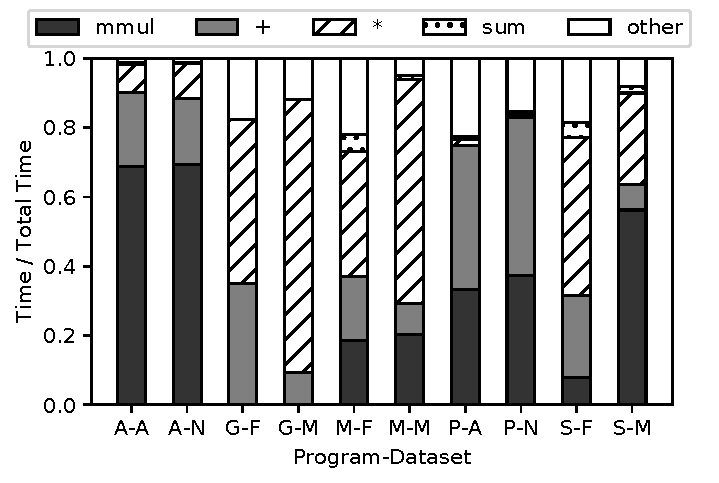
\includegraphics[width=0.8\linewidth]{heavy.pdf}
    \caption{\rvt{Run-time profile of benchmark programs.}}
    \label{heavy}
    \vspace*{5pt}
\end{figure}
Figure~\ref{eval} shows the program run time under \sys\ optimization against SystemML's
optimization. 
 \sys\ is competitive with the hand-coded rules
in SystemML: for GLM and SVM, \sys\ discovers the same
optimizations as SystemML does. For ALS, MLR and PNMF,
\sys\ found new optimizations that lead to \rvo{up to 10X speedup}.
We next analyze each benchmark in detail. 
\begin{figure}
    \centering  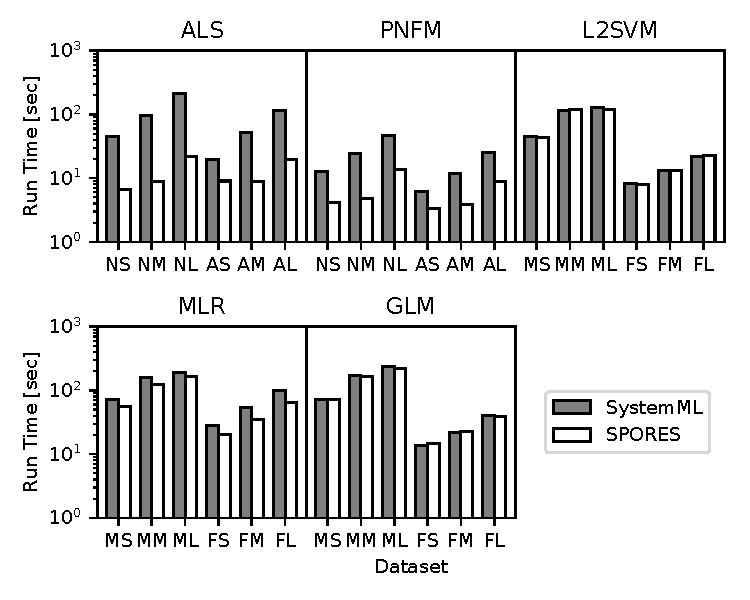
\includegraphics[width=0.9\linewidth]{runtime.pdf}
    \caption{\rvo{Run time under SystemML/SPORES compilation.}} 
    \label{eval}
    \vspace{5pt}
\end{figure}

% \begin{figure}[t]
% \begin{lstlisting}[language=R]
% H=H*(t(W)%*%(X/(W%*%H+eps)))/t(colSums(W))
% W=W*((X/(W%*%H+eps))%*%t(H))/t(rowSums(H))
% obj=sum(W%*%H)-sum(X*log(W%*%H+eps))
% \end{lstlisting}
%     \caption{PNMF main loop. $X$ is a sparse matrix, $W$ and $H$ are low-rank matrices, and
%       $eps$ is a scalar.}
%     \label{pnmf}
% \end{figure}
% \begin{figure}[t]
% \begin{lstlisting}[language=R]
% Q=P[,1:K] * (X %*% ssX_V)
% HV=t(X)%*%(Q - P[,1:K]
%       *(rowSums(Q)%*%matrix(1,1,K)))
% \end{lstlisting}
%     \caption{Part of MLogReg main loop. $X$ and $ssX\_V$ are matrices. In our experiment $K=1$ so
%       $P[,1:K]$ and $Q$ are column vectors, and $matrix(1,1,K)$ is a 1x1
%       matrix holding the value $1$. }
%     \label{mlogreg}
% \end{figure}



% TODO no section 
% \subsection{Rewrite Details} \label{optdetails}

For \textbf{ALS}, SPORES leads to up to 10X speedup beyond SystemML's
optimizations using our relational rules. Investigating the optimized code
reveals the speedup comes from a rather simple optimization: SPORES expands
$(UV^T - X)V$ to $UV^TV-XV$ to exploit the sparsity in $X$. Before the optimization,
all three operations (2 matrix multiply and 1 minus) 
in the expression create dense intermediates because $U$
and $V$ are dense. After the optimization, $XV$ can be computed efficiently thanks to
the sparsity in $X$. $UV^TV$ can be computed in one go without intermediates, taking advantage of
SystemML's \texttt{mmchain} operator for matrix multiply chains. Although the
optimization is straightforward, it is counter-intuitive because one expects
computing $A(B + C)$ is more efficient than $AB + AC$ if one does not consider
sparsity. For the same reason, SystemML simply does not consider distributing
the multiplication and misses the optimization.

For \textbf{PNMF}, the \rvo{speedup of up to 3.5X} using RA rules attributes to rewriting $sum(WH)$
to $sum_{col}(W) \cdot sum_{row}(H)$ which avoids materializing a dense
intermediate $WH$. Interestingly, SystemML includes this rewrite rule but did
not apply it during optimization. In fact, SystemML only applies the rule when
$WH$ does not appear elsewhere, in order to preserve common subexpression.
However, although $WH$ is shared by another expression in PNMF, the other
expression can also be optimized away by another rule. Because both rules uses heuristics to favor sharing CSE, neither fires. 
This precisely
demonstrates the limitation of heuristics. 

For \textbf{MLR}, \sys\ leads to \rvo{up to 1.3X speedup}. The important optimization\footnote{Simplified here for
  presentation. In the source code $P$ and $X$ are not variables but consist of
  subexpressions. } is $P * X - P * sum_{row}(P) * X$ to
$P*(1-P)*X$, where $P$ is a column vector. This takes advantage of the
\texttt{sprop} fused operator in SystemML to compute $P*(1-P)$, therefore
allocating only one intermediate. Note that the optimization factors out $P$, which
is the exact opposite to the optimization in ALS that distributes multiply. Naive
rewrite rules would have to choose between the two directions, or resort to
heuristics to break ties. 

% TODO check dimensions
% \begin{figure}[t]
% \begin{lstlisting}[language=R]
% out=1-Y*(Xw+step_sz*Xd);
% sv=(out>0);
% out=out*sv;
% g=wd+step_sz*dd-sum(out*Y*Xd); 
% h=dd+sum(Xd*sv*Xd);
% step_sz = step_sz - g/h;
% \end{lstlisting}
%     \caption{Part of L2SVM main loop. }
%     \label{l2svm}
% \end{figure}
% \begin{figure}[t]
% \begin{lstlisting}[language=R]
% t_gp=1.0/(1.0+abs(flt)*0.231641888)
% pt_gp = t_gp * ( 0.254829592 
%       + t_gp * (-0.284496736 
%       + t_gp * ( 1.421413741 
%       + t_gp * (-1.453152027 
%       + t_gp *   1.061405429))));
% \end{lstlisting}
%     \caption[gauss error function]{
%     Part of GLM main loop (approximates the Gauss error function~\cite{abramowitz+stegun}). $t\_gp$ is a matrix.}
%     \label{glm}
% \end{figure}
\rvb{
In summary, \sys\ improves performance consistently for ALS, PNMF and MLR across
different data sizes. The impact of sparsity on performance can be gleaned from the particular optimizations: ALS optimization takes advantage of sparsity, while PNMF and MLR optimizations apply for either dense or sparse inputs. }

For \textbf{SVM} and \textbf{GLM}, equality saturation finds the same optimizations as
SystemML does, leading to speedup mainly due to operator fusion. Upon
inspection, we could not identify better optimizations for \textbf{SVM}. For
\textbf{GLM}, however, we discovered a manual optimization that should improve
performance in theory, but did not have an effect in practice since SystemML
cannot accurately estimate sparsity to inform execution. 

\begin{figure}
    \centering  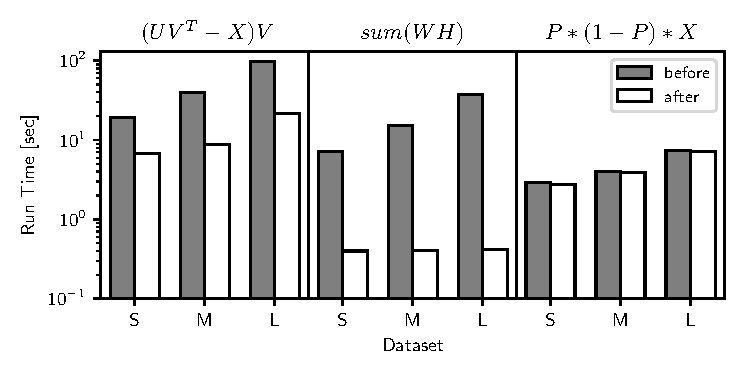
\includegraphics[width=0.9\linewidth]{tf.pdf}
    \caption{\rvb{Run time before- and after-rewrite in TensorFlow.}}
    \label{tfeval}
    \vspace{-10pt}
\end{figure}

\subsubsection*{Comparison Against TensorFlow}
\rvb{
We ran additional experiments in TensorFlow to see if it can also benefit from \sys's
optimizations. For each of the 3 rewrites we discussed in Section~\ref{perf}, we coded
the expressions before- and after-rewrite in TensorFlow. Then we compile each version
with TensorFlow XLA and measure its run time. Figure~\ref{tfeval} shows up to 90X and
50X speedup from the rewrites taken from ALS ($(UV^T-X)V$) and PNMF ($sum(WH)$) respectively. Upon inspection of
the compiled code, we found XLA performs no optimization on the input expressions, likely due
to certain heuristics preferring the unoptimized versions. For MLR ($P*(1-P)*X$),
XLA compiles the before- and after-rewrite expressions to the same code, so the run time
stays the same. We were unable
to compile our full benchmarks with XLA because the latter cannot compile certain operations
on sparse matrices. When this improves, we expect to see \sys\ bring its full potential
to TensorFlow. 
}
\subsection{Compilation Overhead} \label{overhead}
\begin{figure}
    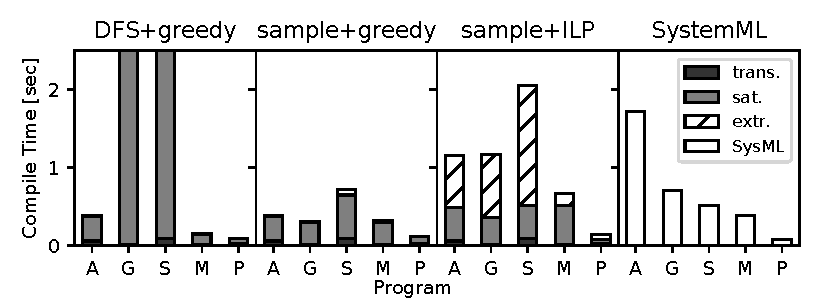
\includegraphics[width=\linewidth]{compiletime.pdf}
    \caption{Compile time breakdown for different saturation and extraction
      strategies. Depth-first saturation reaches the 2.5s timeout compiling GLM and SVM. }
    \label{compile}
    \vspace{5pt}
\end{figure}{}
\begin{figure}
    \centering  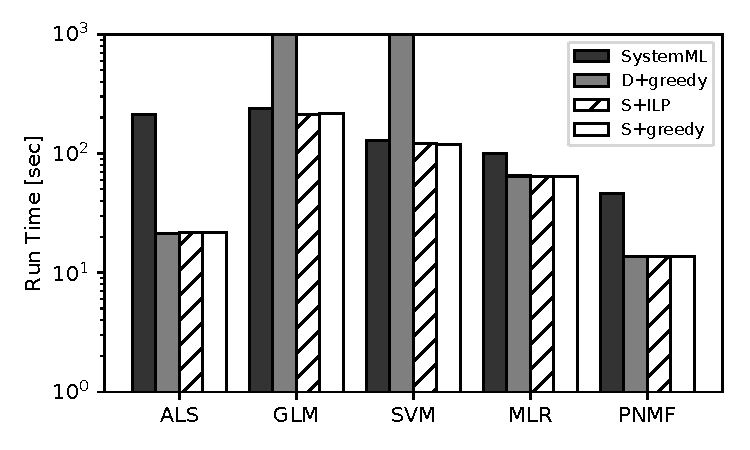
\includegraphics[width=0.8\linewidth]{strategy.pdf}
    \caption{\rvo{Performance impact of different saturation and extraction
      strategies. S is saturation with sampling, and D is depth-first saturation. Depth-first saturation runs into timeout compiling GLM and SVM.}} 
    \label{sampleeval}
\end{figure}

% TODO find number \textcolor{red}{TODO fix caption}}
In our initial experiments, SPORES induces nontrivial compilation
overhead compared to SystemML's native rule-based rewrites. Figure~\ref{compile}
 (sampling, ILP extraction) shows the compile time breakdown for each benchmark, and the majority of time is
spent in the ILP solver. We therefore experiment with the greedy algorithm 
described in Section~\ref{extraction}
 to see if we can trade off guarantees of optimality for a shorter
compile time. Figure~\ref{sampleeval}
shows the performance impact of greedy extraction, and Figure~\ref{compile} (sampling, greedy extraction)
shows the compile time with it. Greedy extraction significantly reduces compile
time without sacrificing \textit{any} performance gain! This is not surprising
in light of the optimizations we discussed in Section~\ref{perf}: all of
these optimizations improve performance regardless of common
subexpressions, so they are selected by both the ILP-based and the greedy
extractor.

We also compare saturation with sampling against depth-first saturation in terms of
performance impact and compile time. Recall the depth-first saturation strategy
applies all matches per rule per iteration. As Figure~\ref{compile} shows,
sampling is slightly slower for ALS, MLR and PNMF, but resolves the timeout for 
GLM and SVM. This is because sampling takes longer to converge when full
saturation is possible, and otherwise prevents the graph from blowing up before
reaching the iteration limit.
Indeed, saturation converges for ALS, MLR and PNMF, which means SPORES
can guarantee the optimality of its result under the given cost model. Saturation
does not not converge before reaching the iteration limit for GLM and SVM because
of deeply nested $*$ and $+$ in the programs. 
Convergence
may come as a surprise despite E-Graph's compaction -- expansive rules like
associativity and commutativity commonly apply in practice. However, the expression
DAGs we encounter are often small (no more than 15 operators), and large DAGs
are cut into small pieces by optimization barriers like uninterpreted functions. 

Figure~\ref{compile} compares the overall DAG compilation overhead of SystemML
against SPORES with different extraction strategies.
Note that the overhead of SystemML also includes optimizations unrelated to sum-product rewrites that are difficult to disentangle, therefore it only gives a sense of the base compilation time and does not serve as head-to-head comparison against SPORES. 
Although SPORES induces significant compilation overhead in light of the total DAG compilation time of SystemML, the overhead is afforded by
its performance gain. As we did not focus our efforts on
reducing compile time, we believe there is plenty room for improvement, for
example organizing rewrite rules to speed up saturation.

\subsection{Numerical Considerations} \label{evaldisc}
\rvt{
Although our rewrite rules preserve semantics for the reals, they do not
preserve semantics under floating point arithmetics. We therefore run experiments
to see if \sys\ sacrifices numerical accuracy. For L2SVM, we
compare the accuracy of the trained model under \sys\ / SystemML optimization; for
MLR and GLM we compare the $R^2$ value; PNMF and ALS terminate after some loss
falls below a threshold, therefore we compare the number of iterations until
termination. Table~\ref{tab:numeric} shows all these statistics are identical under
\sys\ / SystemML optimzation. Although \sys\ does not optimize for numerical accuracy,
equality saturation was used by Herbie \cite{DBLP:conf/pldi/PanchekhaSWT15} for that
exact purpose. We are actively collaborating with Herbie's authors to develop a
multi-objective optimizer for accuracy and run time. 
}
\begin{table}
    \centering
    \caption{\rvt{Numerical characteristics of compiled programs.}}
    \vspace*{7pt}
\scalebox{0.8}{
    \begin{tabular}{l|c|c|c|c}
    \hline
        Optimizer & SysML & SPORES & SysML & SPORES  \\
        \hline
        \hline
        Dataset & \multicolumn{2}{c|}{Airline} & \multicolumn{2}{c}{MNIST} \\
        \hline
        SVM ($acc.$) & $82.4\%$ & $82.4\%$ & $96.8\%$ & $96.8\%$ \\
        \hline
        MLR ($R^2$) & $0.773$ & $0.773$ & $0.742$ & $0.742$ \\
        \hline
        GLM ($R^2$) & 0.618 & 0.618 & 0.671 & 0.671 \\
        \hline
        \hline
        Dataset & \multicolumn{2}{c|}{Netflix} & \multicolumn{2}{c}{Amazon} \\
        \hline
        PNMF ($iter.$) & 18 & 18 & 36 & 36 \\
        \hline
        ALS ($iter.$) & 8 & 8 & 9 & 9 \\
        \hline
    \end{tabular}}
    \label{tab:numeric}
    \vspace*{5pt}
\end{table}{}

\section{Related Work}

% TODO emphasize SystemML
% TODO ADD Immanual Trummer, PILP
% Morpheus
% lara
% volcano
There is a vast body of literature for both relational query optimization and
optimizing compilers for machine learning. Since we optimize machine learning programs through a
relational lens, our work relates to research in both fields. As we have pointed
out, numerous state-of-the-art optimizing compilers for machine learning
 resort to syntactic rewrites and heuristics to optimize linear algebra
expressions~\cite{DBLP:reference/bdt/Boehm19}~\cite{DBLP:conf/icml/SujeethLBRCWAOO11}~\cite{DBLP:conf/sigmod/HuangB013}. We distinguish our work which performs optimization based on a
relational semantics of linear algebra and holistically explore the complex
search space. A majority of relational query optimization focus on join order
optimization \cite{Graefe95a} \cite{MoerkotteN06} \cite{MoerkotteN08}
\cite{selinger1979access}; we distinguish our work which optimizes programs with
join (product), union (addition), and aggregate (sum) operations. Sum-product optimization considers operators other than join while optimizing
relational queries. Recent years have seen a line of excellent theoretical and
practical research in this area \cite{KhamisNR16} \cite{Joglekar2016AJARAA}.
These work gives significant improvement for queries involving $\times$ and $\sum$,
but fall short of LA workloads that occur in practice. We step past these
frameworks by incorporating common subexpressions and incorporating addition
($+$). 

In terms of approach, our design of relational IR ties in to research that
explores the connection between linear algebra and relational algebra. Our
design and implementation of the optimizer ties into research that leverage
equality saturation and \textsc{and-or dag}s for query optimization and compiler
optimization for programming languages. Since we focus on optimizing sum-product
expressions in linear algebra, our work naturally relates to research in sum-product
optimization. We now discuss these three lines of research in detail. 

\subsection{Relational Algebra and Linear Algebra}
Elgamal et al. \cite{ElgamalLBETRS17} envisions \textsc{spoof}, a compiler for machine learning programs
that leverages relational query optimization techniques for LA sum-product optimization. 
We realize this vision by providing the translation
rules from LA to RA and the relational equality rules that completely represents
the search space for sum-product expressions. One important distinction is, Elgamal
et al. proposes \emph{restricted relational algebra} where every expression must
have at most two free attributes. This ensures every relational expression in every step of the
optimization process to be expressible in LA. In contrast, we remove this restriction and only require the 
optimized output to be in linear algebra. This allows us to trek out to spaces not
covered by linear algebra equality rules and achieve completeness. In addition 
to sum-product expressions, Elgamal et al. also considers selection and projection operations
like selecting the positive entries of a matrix. We plan to explore supporting
selection and projection in the future. Elgamal et al. also proposes compile-time generation of
fused operators, which is implemented by Boehm et al.~\cite{DBLP:journals/pvldb/BoehmRHSEP18}.
SPORES readily takes advantage of existing fused operators, and we
plan to explore combining sum-product rewrite with fusion generation in the future. 

MorpheusFI by Li et al.~\cite{DBLP:conf/sigmod/LiC019} and LARA by Hutchison et al.~\cite{DBLP:journals/corr/HutchisonHS17} explore optimizations across the interface of machine learning and database systems. In particular, MorpheusFI speeds up machine learning algorithms over large joins by pushing computation into each joined table, thereby avoiding expensive
materialization. LARA implements linear algebra operations with relational operations and
shows competitive optimizations alongside popular data processing systems. 
Schleich et al.\cite{DBLP:conf/sigmod/SchleichOC16} and Khamis et al.\cite{DBLP:journals/corr/NgoNOS17} explore in-database learning, which aims to push entire
machine learning algorithms into the database system. 
We contribute in this space by showing that even without a relational engine, the
relational abstraction can still benefit machine learning tasks as a powerful
intermediate abstraction. \rvt{Kotlyar et.al. \cite{DBLP:conf/europar/KotlyarPS97}
explore compiling sparse linear algebra via
a relational abstraction. We contribute by providing a simple set of rewrite rules
and prove them complete.}

\subsection{Equality Saturation and AND-OR DAGs}
Equality saturation and \textsc{and-or dag}s have been applied to optimize
low-level assembly code~\cite{DBLP:conf/pldi/JoshiNR02}, Java programs \cite{DBLP:journals/corr/abs-1012-1802}, 
database queries \cite{Graefe95a}, floating point arithmetics \cite{DBLP:conf/pldi/PanchekhaSWT15}, and even computer-aided
design models \cite{DBLP:journals/corr/abs-1909-12252}. The design of our relational IR brings unique challenges
in adopting equality saturation. Compared to database query optimizers 
that focus on optimizing join orders, unions and aggregates play a central
role in our relational IR and are prevalent in real-world programs. As
a result, our
equality rules depend on the expression schema which is not immediately accessible
from the syntax. We propose class invariants as a solution to access schema
information, and show it to be a powerful construct that enables constant
folding and improves cost estimation. Compared to optimizers for low-level
assembly code or Java program, we commonly encounter linear algebra expressions
that trigger expansive rules and make saturation convergence impractical. 
We propose to sample rewrite matches in order to achieve good exploration
without full saturation. Equality saturation takes advantage of constraint solvers which have also been applied to program optimization and query
optimization. In particular, the use of solvers for satisfiability
modulo theories by \cite{DBLP:conf/asplos/Solar-LezamaTBSS06} has spawned a paradigm now known as \textit{program synthesis}. 
In query optimization research, 
\cite{DBLP:conf/sigmod/Trummer017} applies Mixed Integer Linear Programming for optimizing join ordering. 
Although constraint solvers offer pleasing guarantees of optimality, our
experiments show their overhead does not bring significant gains for optimizing
LA expressions. 

\subsection{Low-level Code Generation}
\rvt{
Novel machine learning compilers including TACO \cite{DBLP:journals/pacmpl/KjolstadKCLA17},
TVM \cite{DBLP:conf/nips/ChenZYJMCGK18}, TensorComprehension \cite{DBLP:journals/corr/abs-1802-04730} and
Tiramisu \cite{DBLP:conf/cgo/BaghdadiRRSAZSK19} generate efficient low-level code
for kernel operators. These kernels are small expressions that consist of a few
operators. For example the MATTRANSMUL kernel in TACO implements $\alpha A^T x + \beta z$.
The kernels are of interest because they commonly appear in machine learning programs,
and generating efficient low-level implementation for them can greatly impact performance. 
However, these compilers cannot perform algebraic rewrite on large programs as \sys\ does.
For example, TACO
supports only plus, multiply and aggregate, whereas \sys\ supports any custom functions
as discussed in Section~\ref{udfs}; Tiramisu requires tens of lines of code just to
specify matrix multiply which is a single operator in \sys. Furthermore, the basic polyhedral
model in Tiramisu and TensorComprehension does not support sparse matrices. Sparse extensions exist, but require the
user to make subtle tradeoffs between expressivity and performance \cite{DBLP:journals/pieee/StroutHO18}.
At a high level,
we view these kernel compilers as complementary to \sys. The former can provide efficient kernel
implementation just like the fused operators in SystemML, and we can easily include these
kernels in \sys\ for whole-program rewrite. The TASO compiler \cite{DBLP:conf/sosp/JiaPTWZA19}
combines kernel-level rewrite with whole-program rewrite, and is
also driven by a set of equality rules like \sys. However, it induces significant overhead --
generating operator graphs with just up to 4 operators takes 5 minutes, and while \cite{DBLP:conf/sosp/JiaPTWZA19}
does not include detailed time for compiling whole programs, it reports the compilation
finishes in ``less than ten minutes''. In contrast, \sys\ takes seconds instead of minutes
in compilation.} 

% \subsection{Exploiting Sparsity}
% A number of optimizing compilers for linear algebra programs support sparse
% matrix operators . SystemML \cite{boehm2014systemml} and Cumulon
% \cite{DBLP:conf/sigmod/HuangB013} includes a variety of hand-fused sparse operators.
% \cite{ElgamalLBETRS17} further automates the generation of fused operator
% implementation. However, all existing approach either work on a per-operator
% basis, or rely on hand-coded rules to rewrite expressions to fused operators.
% Using equality saturation, we can automatically discover opportunity for
% operator fusion based on a simple set of equality rules. And even with the
% absence of operator fusion, we can still take advantage of sparsity in our
% optimization.

% \subsection{Multi-query Optimization}
% The research in Multi-query Optimization aims to share common subqueries among
% multiple queries to speed up processing \cite{Kathuria017}. This is closely
% related to our problem of exploiting CSEs in linear algebra, although our focus
% is intra-query instead of inter-query. Moreover, the majority of multi-query
% optimizers focus on joins, whereas union and aggregate are essential for linear
% algebra programs. One lesson we can learn from the literature multi-query
% optimization is to perform equality saturation for multiple expressions in the
% same egraph, thereby enabling sharing across optimization sessions and reducing
% compilation time.

\section{Limitations and Future Work}
\rvt{
We intend \sys\ to be used to optimize machine learning programs that perform
linear algebra operations. As such, \sys\ is not a linear algebra solver, and 
operations like matrix inversion and calculating eigenvalues are out of scope.
\sys\ does not include a matrix decomposition operator, but the programmer
can implement decomposition algorithms like our ALS and PNMF benchmarks. 
The operations we support already cover a variety of algorithms as we show in
the evaluation. Similar scope is shared by existing research \cite{DBLP:journals/pvldb/BoehmRHSEP18}
\cite{ElgamalLBETRS17}
\cite{DBLP:journals/pacmpl/KjolstadKCLA17}. Although
\sys\ does not focus on deep learning, its design can be adapted to optimize
deep models. We are experimenting to incorporate the identity rules from TASO
into our framework. It would be challenging to extend the completeness theorem to
the complex operators used in deep learning, 
but we expect our extension of equality saturation can find high-impact optimizations
with short compile time. Finally, although our rewrite rules are complete, we had to
resort to rule sampling and greedy extraction to cut down the overhead. Future work can 
investigate more intelligent rule application and extraction strategies. For example,
the optimizer can learn which rules more likely lead to performance improvement and
prioritizes firing those rules. Another direction is to incorporate plus into
theoretical sum-product frameworks like FAQ \cite{KhamisNR16} and guarantee optimality. 
}

\chapter{Optimizing Recursive Queries}
\label{chapter:fgh}

Most database systems are designed to support primarily non-recursive
(loop-free) queries.  Their optimizers are based on the rule-driven,
cost-based Volcano architecture, designed specifically for optimizing
non-recursive query plans.  However, most data science and machine
learning workloads today involve some form of recursion or iteration.
Examples include finding the connected components of a graph,
computing the page rank, computing the network centrality, minimizing
an objective function using gradient descent, etc.  The importance of
supporting recursive queries has been noted by system designers.
Some modern data analytics systems, like Spark or Tensorflow, support
for-loops. The SQL standard defines a limited
%  \footnote{The recursion is limited to a single IDB, with a single recursive rule,
%   and the rule must be linear.}
form of recursive queries, using the
\texttt{with} construct, and some popular engines, like Postgres or
SQLite, do support this restricted form of recursion.

%
The Datalog language, covered in Chapter~\ref{chap:background}, is
designed specifically for recursive queries, and it is gaining in
popularity~\cite{DBLP:conf/datalog/AlvaroMCHMS10,
DBLP:reference/db/RoscoeL18,
10.1145/3452021.3458815,
10.1145/1989323.1989456,
BigDatalog,
DBLP:journals/pvldb/FanZZAKP19,
DBLP:journals/tkde/SeoGL15,
10.14778/2824032.2824052,
francislandau-vieira-eisner-2020-wrla}.
But the optimization problem for recursive queries is
much less studied.  
The na\"ive evaluation of Datalog repeatly applies the 
 rules in a loop, until a fixpoint is reached. 
% A  Datalog program consists of multiple rules,
% defining several, mutually recursive relations, and one
% distinguished relation name which is the output of the program.  The
% effect of the program consist of repeatedly applying the rules,
% sometimes called the {\em body} of the program, until a fixpoint is
% reached, then it returns the output relation.
% A recursive query consists of some non-recursive
% expression, the {\em body}, which is evaluated repeatedly, in a loop,
% until either a fixpoint is reached, or some convergence criterion is
% met.  
Datalog engines typically optimize the loop body, without optimizing
the actual loop.  The few systems that do,
% (for example Soufflé) 
apply only limited optimization techniques, like magic set optimization and
semi-naive evaluation, which are restricted to positive queries.

In this chapter we describe a new query optimization framework for
recursive queries.  Our framework replaces a recursive program with
another, equivalent recursive program, whose body may be quite
different, and thus focuses on optimizing the recursive program as a
whole, not on optimizing its body in isolation; the latter can be done
separately, using standard query optimization techniques.  Our
optimization is based on a novel rewrite rule for recursive programs,
called the FGH-rule, which we implement using {\em program synthesis},
a technique developed in the programming languages and verification
communities. We introduce a new method for inferring loop invariants,
which extends the reach of the FGH-rule, and also show how to use
global constraints on the data for semantic optimizations using the
FGH-rule.  
% We explain these points in some details next.


{\bf The FGH-Rule} At the core of our approach is a novel, yet very
simple rewrite rule, called the FGH-rule (pronounced {\em fig-rule}),
which can be used to prove that two recursive programs are equivalent,
even when their loop bodies are quite different.  We show that the
FGH-rule can express previously known optimizations for Datalog,
including magic sets and semi-naive evaluation, and also a wide range
of new optimizations.  The optimized program is often significantly
more efficient than the original program, and sometimes can have a
strictly lower asymptotic complexity.  We implemented a
source-to-source optimizer using the FGH-rule, evaluated its
effectiveness on several Datalog systems, and observed speedups of up
to $4$ orders of magnitude (Sec.~\ref{sec:eval}).

For a taste of the FGH-optimization, consider the following example,
from~\cite{DBLP:journals/tplp/ZanioloYDSCI17,DBLP:conf/amw/ZanioloYIDSC18}:
compute the connected components of an undirected graph $E(x,y)$.  The
Datalog program in Fig.~\ref{fig:cc} (a) achieves this by first
computing the transitive closure relation $TC(x,y)$, then computing a
$\min$-aggregate query
assigning to every node $x$ the smallest label $L[y]$ of all nodes $y$ reachable from $x$.
In contrast, the optimized program in Fig.~\ref{fig:cc} (b)
computes directly the CC label of every node $x$ as the  minimum of its own label
and the smallest CC label of its neighbors,
using a single recursive rule with
$\min$-aggregation.
The space complexity of the transitive closure is
$O(n^2)$, which, in practice, is prohibitively expensive on large graphs.
On the other hand, the optimized query has space complexity $O(n)$.

\begin{figure}
  \centering
% \fcolorbox{black}{light-gray}{\parbox{0.45\textwidth}{
\begin{align*}
  TC(x,y) \cd &  [x=y] \vee \exists z(E(x,z) \wedge TC(z,y)) \\
  CC[x] \cd & \min_y \setof{L[y]}{TC(x,y)}
\end{align*}
% }}
% \newline
\null\hfill(a)\hfill\null

% \fcolorbox{black}{light-gray}{\parbox{0.45\textwidth}{
\begin{align*}
  CC[x] \cd & \min(L[x], \min_y \setof{CC[y]}{E(x,y)})
\end{align*}
% }}
% \newline
\null\hfill(b)\hfill\null

\caption{Unoptimized (a) and optimized (b) Datalog program for the connected components of an undirected graph.}
  \label{fig:cc}
\end{figure}


{\bf Pattern Matching vs.\ Query Synthesis} Applying the FGH-rule is
an instance of {\em query rewriting using views}.  In that problem we
are given a set of view expressions and a query, and the task is to
rewrite the query to use the view expressions rather than the base
relations. This problem has been extensively studied in the
literature~\cite{DBLP:journals/vldb/Halevy01}, and today's database
systems perform it using pattern
matching~\cite{DBLP:conf/sigmod/GoldsteinL01}.  This is a form of
transformational synthesis, where every candidate query rewriting is
guaranteed to be correct, because it is obtained by applying a limited
set of manually crafted rules (patterns), which are guaranteed to be
correct.  However, the FGH-rule often requires exploring a very large
space, which cannot be covered by a limited set of rules.  In this
paper we propose to use for this purpose {\em counterexample-guided inductive
  synthesis} (\cegis), a technique designed
for program
sketching~\cite{DBLP:conf/asplos/Solar-LezamaTBSS06,DBLP:conf/tacas/TorlakJ07}.
When applied to our context, we call this technique {\em query
  synthesis}.  Unlike pattern matching, query synthesis explores a
much larger space, by examining rewritings that are not necessarily
correct, and need to be checked for correctness by a verifier (\zzz\ in
our system).
The verifier also produces a small counterexample
database for each rejected candidate, and these counterexamples are
collected by the synthesizer and used to produce only candidate
rewritings that pass all the previous counterexamples, which
significantly prunes the search space of the synthesizer.  We report
in Sec.~\ref{sec:eval} synthesis times of less than 1 second, even for
complex queries that use global constraints and require inferring loop
invariants.

% \reinhard{Do the results in Sec.~\ref{sec:eval} really report run times in seconds? I thought
% the numbers are to be interpreted as percent relative to the run time of the unoptimized program?!}

%  \hqn{Perhaps briefly mention the idea that ``transformational synthesis'' is
%  in some sense an under approximation of the search space, while CEGIS
%  is an over approximation.}

{\bf Monotone Queries and Semiring Semantics} Datalog is, by
definition, restricted to monotone queries.
% This ensures that every
% query has a well-defined semantics, namely the least fixpoint of its
% immediate consequence operator.  Existing optimizations for Datalog,
% like semi-naive evaluation and magic set rewriting, apply mainly to
% monotone queries. Even stratified negation can (if at all)
% only be handled by imposing appropriate restrictions~\cite{DBLP:journals/corr/abs-1909-08246}.
%\hqn{There are a couple of papers~\cite{DBLP:journals/jlp/BalbinPRM91,DBLP:journals/corr/abs-1909-08246} with magic set transforms on queries with
%negations. Need to check what kind of stratification assumption is needed.}
%\reinhard{Hung, are you happy with the above formulation on stratified negation?}
% From Hung, YES : thanks Reinhard
But queries that contain aggregates or negation
(expressed in SQL via subqueries) are not monotone, and most systems
that support recursion prohibit the combination of aggregates and
recursion.  This has two shortcomings: it limits what kind of queries
the user can express, and also prevents many of our FGH-rewritings.
For example, the simple computation of connected components in
Fig.~\ref{fig:cc} (a) can be expressed in PostgreSQL, or in SQLite, or
in Soufflé,
% \footnote{These systems have a different syntax than in our
%   paper, but expressing the query in Fig.~\ref{fig:cc} (a) in any of
%   these systems is straightforward.}
because the first rule uses
only recursion and the second rule uses only aggregation.  However,
none of these systems accepts the query in Fig.~\ref{fig:cc} (b),
because it combines recursion and aggregation.\footnote{Prior
  work~\cite{DBLP:conf/pods/GangulyGZ91,DBLP:journals/tkde/SeoGL15}
  has proposed extending Datalog with $\min$ and $\max$ aggregates by
  explicitly re-defining the semantics of recursive rules with
  aggregates.  Our approach keeps the standard least fixpoint
  semantics, but generalizes the semiring.}  
In order to express such queries, we work with the \datalogo
 language introduced in Chapter~\ref{chap:datalogo}
that supports recursive aggregates by extending Datalog with semirings.

% in this chapter we propose an extension of Datalog, following
% the approach in~\cite{DBLP:conf/pods/GreenKT07}, where the relations
% are interpreted over {\em ordered semirings}.

% A semiring is an
% algebraic structure with two operations, $\oplus, \otimes$.
% Traditional Datalog corresponds to the Boolean semiring, where these
% two operators are $\vee, \wedge$, while the query in Fig.~\ref{fig:cc}
% (b) is over the Tropical semiring, where the two operators are
% $\min, +$ (reviewed in Sec.~\ref{sec:background}).
% We call this extension of Datalog to ordered semirings $\name$,
% pronounced ``Datalogo'', where the circle represents
% the semiring.  In $\name$ recursion is still restricted to monotone\footnote{This
% monotonicity is over the partial order from the ordered semiring.}
% queries, but monotone queries in $\name$ include queries with aggregates, over an
% appropriate semiring.  The query in Fig.~\ref{fig:cc} (b) is monotone
% over the (ordered) tropical semiring.

{\bf Loop Invariants} One difficulty in reasoning about loops in
programming languages is the need to discover loop invariants.  Some
(but not all) applications of the FGH-rule also require the discovery
of loop invariants.  We describe a novel technique for inferring loop
invariants for $\name$ programs, by combining symbolic execution with
equality saturation, and using a verifier.  We execute symbolically
the recursive program for a very small number of iterations (five in
our system), obtain query expressions for the IDBs (the recursive
predicates), and construct all identities satisfied by the IDBs.
Then, we retain only candidates that hold at each iteration, and check
each candidate for correctness using the SMT solver.  By inferring and
using loop invariants we show that we can significantly improve some
instances of magic-set optimizations from the literature: we call the
new optimization {\em beyond magic}.




% .  Each such identity is
% a candidate for a loop invariant, and we check it using a verifier.
% The challenge with this approach is the fact that the space of
% candidate invariants is very large, even infinite.  For the program
% in Fig.~\ref{fig:cc} (a), if we examine all identities satisfied at
% iteration 0, then $TC = \emptyset$, and any combination of
% joins of $TC$ and $E$ with at least one occurrence of $TC$ is empty,
% leading to an infinite set of equivalent expressions.  To cope with a
% potentially infinite space, we use a state-of-the art {\em equality
%   saturation system}
% (\eqsat)~\cite{DBLP:journals/pacmpl/WillseyNWFTP21}, which uses a
% finite representation of an infinite equivalence class.  This
% technique allows us to discover non-trivial loop invariants, which
% leads to powerful optimizations of recursive queries.  We also use
% the \eqsat\ system in several other places in our optimizer as we shall
% explain (see also Fig.~\ref{fig:arch}).


{\bf Constraints and Semantic Optimizations} Optimizations that are
conditioned on certain constraints on the database are known as {\em
semantic optimizations}~\cite{DBLP:journals/debu/RamakrishnanS94}.
SQL optimizers routinely use key constraints and foreign key
constraints to optimize queries.  More powerful optimizations can
be performed using the chase and back-chase
framework~\cite{DBLP:conf/vldb/DeutschPT99,DBLP:conf/sigmod/PopaDST00},
and these include optimizations under inclusion constraints, or
conditional functional dependencies, or tuple generating constraints.
However, all constraints that are useful for optimizing non-recursive
queries are {\em local}.  In contrast, the FGH-rule optimizes
recursive queries, and therefore it can also exploit {\em global}
constraints.  For example, suppose the database represents a graph,
and the global constraint states that the graph is a tree.  This
global constraint does not help optimize non-recursive queries, but
can be used to great advantage to optimize some recursive queries; we
give details in Sec.~\ref{subsec:constraints}.

{\bf Equality Saturation} Throughout our optimizer we need to
manage symbolic expressions of queries, and their equivalence classes,
as defined by a set of rules.  
This is achieved once again with equality saturation (\eqsat), 
 a technique introduced in Chapter~\ref{chapter:spores}.
We show how to use
\eqsat\ for checking equality under constraints, inferring loop
invariants, and ``denormalization'' (which is essentially query
rewriting using views).



%  For example, suppose
% the query computes for each node the number of its descendants.  If
% the query is written without this constraint in mind, then it needs to
% first compute the transitive closure of the graph, then compute a
% $\texttt{group-by, count(*)}$ on the transitive closure relation.  Our
% optimizer can use the tree-constraint and optimize this query into one
% that computes the number of descendants recursively, bottom up, in a
% single pass over the tree.



% To apply the FGH-rule, the optimizer
% needs to perform two steps: {\em synthesize} a candidate query, then
% {\em verify} the FGH-rule.  This is in contrast to traditional query
% optimizers, whose task is restricted to simply enumerating equivalent
% query plans by repeatedly apply rewrite rules from a knowledge base of
% rules.  Both program synthesis and verification of expression
% equivalence has been studied extensively in the programming language
% and verification
% communities~\cite{DBLP:conf/asplos/Solar-LezamaTBSS06,DBLP:conf/tacas/TorlakJ07}.
% Our approach adopts and extends some of those techniques to the
% specific task of synthesizing queries for the FGH-rule.  We use
% Rosette~\cite{DBLP:conf/oopsla/TorlakB13} and adopt the
% Conterexample-Guided Inductive Synthesis
% (CEGIS)~\cite{DBLP:conf/asplos/Solar-LezamaTBSS06} approach for
% synthesis, and use the EGG {\em equality saturation}
% system~\cite{DBLP:journals/pacmpl/WillseyNWFTP21} and \zzz~\cite{?????}
% for verification.

% dan{I'm not sure whether to keep the next paragraph}
%
% \bf Scope} There are three scenarios encountered in practice when
% pplying the FGH-rule is highly effective.  The first is when the
% ystem provides a library of recursive queries, and the user computes
%  final answer by applying some function on the result of the
% ecursive program.  In the connected-component example in
% ig.~\ref{fig:cc} (a), the recursive transitive-closure program may be
% rovided by the systems library, and the user only writes the second
% ine of the program.  Other examples include {\em magic set
%  optimizations}~\cite{DBLP:conf/pods/BancilhonMSU86,DBLP:conf/sigmod/MumickP94,DBLP:conf/sigmod/MumickFPR90},
% here a selection predicate is applied to the result of a recursive
% uery, and the $\prem$ condition for pushing aggregates over
% ecursion~\cite{DBLP:journals/tplp/ZanioloYDSCI17}.  The second
% cenario is when the optimized program is not expressible in the
% anguage supported by the system.  For example, the program in
% ig.~\ref{fig:cc} (b) is both recursive and requires the computation
% f an aggregate.  The  Datalog system
% ouffle~\cite{DBLP:conf/cav/JordanSS16} supports both recursive rules
%  and aggregates, but does not allow them to be combined.  Thus, the
%  only way to express connected components in Souffle is as
%  in\footnote{The optimizer may still be able to execute the program
%    using a physical plan similar to Fig.~\ref{fig:cc} (b), even if it
%    does not support aggregates in recursive rules in the language.}
%  Fig.~\ref{fig:cc} (a).  Finally, the third scenario is that of {\em
%    semantic optimization}~\cite{DBLP:journals/debu/RamakrishnanS94},
%  when the user's query can be optimized by using constraints over the
%  database.  Semantics optimizations have been studied extensively for
%  traditional, non-recursive queries; one of the best known is when a
%  SQL optimizer uses a key and foreign-key constraint to remove a
%  redundant join operation.  In our settings both the constraints and
%  the optimizations can be richer.  For example, consider the {\em
%    total-cost} problem, where we are given a hierarchy of parts,
%  subparts, sub-subparts, etc, and are asked to compute, for each
%  (sub)part the sum of costs of all its subparts.  The user needs to
%  compute the transitive closure first, because, in general, the
%  hierarchy can be a DAG and we need to avoid double counting of
%  shared subparts.  But given the constraint that the data is a tree,
%  our optimizer can apply the FGH-rule and optimize the program into a
%   simple bottom-up computation, which takes linear time.

% 
% The cited papers also propose techniques to speed up \cegis;
% since we implement our optimizer atop the general \cegis\ system Rosette,
% we can readily benefit from these new techniques when they are
% incorporated in Rosette.

{\bf Contributions} In summary, the main contribution of this chapter
consists of a new, principled and powerful method for optimizing
recursive queries.  We make the following specific contributions:
%
\begin{itemize}
\item We introduce a simple optimization rule for recursive queries,
  called the FGH-rule (Sec.~\ref{sec:fgh}).
\item We show the FGH-rule captures known optimizations (magic
  sets, $\prem$, semi-naive), (Sec.~\ref{subsec:simple:examples}), 
  new optimizations (Sec.~\ref{subsec:loop:invariants}), and
  optimizations under global constraints
  (Sec.~\ref{subsec:constraints}).
\item We present our novel framework for query optimization via
the FGH-rule  (Sec.~\ref{sec:optimization}).
%\item We describe how to check query equivalence using an SMT solver
%  (Sec.~\ref{sec:verification}).
%\item We describe how to perform query synthesis for the FGH-optimizer
%  using a \cegis\ system (Sec.~\ref{subsec:synthesis}).
\item We describe how an SMT solver
(Sec.~\ref{sec:verification}) and a
\cegis\ system (Sec.~\ref{subsec:synthesis})
 % to perform query synthesis
can be profitably integrated into our FGH-optimizer.
\item We describe how to use an \eqsat\ system for various tasks in
  the FGH optimizer: loop-invariant inference, denormalization,
  and checking equivalence under constraints (Sec.~\ref{sec:semantic-opt}).
%%% \item We describe our novel framework using an SMT solver  and an equality saturation
%%%   system for applying the FGH-rule in Sec.~\ref{sec:optimization}.
%%% \item Three crucial parts of our optimization process are described in detail
%%% in Secs.~\ref{sec:verification}, \ref{subsec:synthesis}, and \ref{sec:semantic-opt}:
%%% verification, synthesis, and equality saturation.
%%% \item We conduct an empirical evaluation of our optimization approach
%%%   by performing source-to-source rewritings and measuring their
%%%   effectiveness on several Datalog systems (Sec.~\ref{sec:eval}).
\end{itemize}
% \reinhard{Is the formulation in the penultimate bullet now safe (and not too weak)?}

%\reinhard{Should we mention the (very favorable) experimental results in an additional bullet?}

%%% Local Variables:
%%% mode: latex
%%% TeX-master: "main"
%%% End:

% \section{Background}

% \label{sec:background}

% %We provide here a brief background on Datalog and semirings.

% {\bf Datalog} \update{A {\em relation} of arity $k$ is a finite subset
%   of $D^k$, where $D$ is a fixed domain.  The abbreviations} EDB and
% IDB stand for {\em Extensional Database} and {\em Intensional
%   Database}, and represent the base relations and the computed
% relations respectively.  A {\em rule} has the form:
% %
% \begin{align*}
%   R_0(\texttt{vars}) \cd & R_1(\texttt{vars}_1) \wedge \cdots \wedge R_m(\texttt{vars}_m)
% \end{align*}
% %
% where $R_0$ is an IDB, and $R_1, \ldots, R_m$ are IDBs or EDBs.  The
% rule is {\em safe} if every variable occurs in at least some predicate
% in the body, and the rule is {\em linear} if its body contains at most
% one IDB.  A {\em Datalog program} consists of a set of possibly
% mutually recursive rules.  Usually, only a subset of the IDB
% predicates are returned to the user, and we will call them the {\em
%   answer} IDBs.  The {\em Immediate Consequence Operator}, ICO, is the
% mapping on the IDB predicates that consists of one application of all
% the Datalog rules.  The {\em semantics} of a Datalog program is given
% by the least fixpoint of its ICO.  The {\em naive evaluation
%   algorithm} consists of repeatedly applying the ICO until the IDBs no
% longer change.
% % The
% % {\em semi-naive evaluation algorithm} reduces the number of
% % rediscovered tuples by computing separately
% % $\Delta_n \defeq \bm R_n - \bm R_{n-1}$:
% % \begin{align}
% %   \Delta_0 = \bm R_1 \defeq & P(\emptyset) \nonumber \\
% %   \bm \Delta_n \defeq & \Delta P(\bm R_n, \Delta_{n-1}) - \bm R_n
% %                       & \bm R_{n+1} \defeq & \bm R_n \cup \Delta_n
% % \end{align}
% % %
% % Here $\Delta P$ is the {\em incremental view computation} query,
% % i.e., any expression that satisfies
% % $P(\bm R \cup \Delta) = P(\bm R) \cup \Delta P(\bm R, \Delta)$.  The
% % seminaive program terminates when $\Delta_n=\emptyset$.

% \update{
% %
%   In this chapter we will combine multiple rules with the same head into
%   a single rule by OR-ing their bodies, and writing explicitly all
%   existential quantifiers.  This is a common convention used in the
%   literature, see e.g.,~\cite{DBLP:journals/jlp/Fitting91}.  For
%   example the following  Datalog program, which computes the transitive
%   closure of a relation $E$,
% %
% \begin{align*}
%   TC(x,y) \cd & E(x,y) \\
%   TC(x,y) \cd & E(x,z) \wedge TC(z,y)
% \end{align*}
% %
% becomes $TC(x,y) \cd E(x,y) \vee \exists z (E(x,z) \wedge TC(z,y))$.
% }

% {\bf (Pre-)Semirings} A {\em pre-semiring} is a tuple
% $\bm S = (S, \oplus, \otimes, \zero, \one)$ where \update{$\oplus$ is
%   commutative,} both $\oplus, \otimes$ are associative, have
% identities $\zero$ and $\one$ respectively, and $\otimes$ distributes
% over $\oplus$.  \update{When $\otimes$ is commutative, then we call
%   $\bm S$ a {\em commutative} pre-semiring.  All pre-semirings in this
%   paper are commutative, and we will simply refer to them as
%   pre-semirings.}  When the equality $x \otimes \zero = \zero$ holds
% for all $x$, then it is called a {\em semiring}.  An {\em ordered}
% pre-semiring is a pre-semiring with a partial order $\preceq$, where
% both $\oplus, \otimes$ are monotone operations.  When the partial
% order is defined by $x\preceq y$ iff $\exists z, x\oplus z = y$ then
% it is called the {\em natural order}.  Examples of ordered
% (pre-)semirings are the Booleans
% $\B = (\set{0,1}, \vee, \wedge, 0, 1)$, the closed natural numbers
% $\N^\infty = (\N \cup \set{\infty},+,*,0,1)$, the tropical semiring
% $\trop = (\N \cup \set{\infty}, \min, +, \infty,0)$, the reversed
% tropical semiring $\trop^r=(\N, \max, +, 0, 0)$, the lifted naturals
% and lifted reals $\N_\bot = (\N \cup \set{\bot}, +, *, 0, 1)$,
% $\R_\bot = (\R \cup \set{\bot}, +, *, 0, 1)$, where
% $\bot + x = \bot * x = \bot$.  The structures $\B, \N^\infty, \trop$
% are semirings, the others are pre-semirings.  $\B$,
% $\N^\infty, \trop$, and $\trop^r$ are naturally ordered.  Confusingly
% (!!), the order relation on $\trop$ is the reverse one: $\infty$ is
% the smallest, and $0$ is the largest element.  The order relation in
% $\N_\bot$ and $\R_\bot$ is given by $\bot \preceq x$ for all $x$: they
% are ordered pre-semirings but not naturally ordered.%
% \footnote{Note that we define $\trop$ and $\trop^r$ over the natural
%   numbers rather than the reals. The motivation for this slight
%   deviation from the standard definition of these semirings will
%   become clear in Section \ref{sec:verification}: the support of
%   integer theories by the SMT-solver \zzz.}


% %  \hqn{May need to clarify why we define the tropical semiring over $\N$ instead of $\R$?
% %  The standard definition (from Wikipedia, e.g.) uses $\R$}

% {\bf $\bm S$-relations} An $\bm S$-relation $R$ is a function that
% associates to each tuple $t \in D^k$ a value in the semiring,
% $R[t] \in \bm S$.  In this context, $\bm S$ is called the {\em value
%   space} of the relation $R$, while the domain $D$ of its attributes
% is called the {\em key space}.  $\bm S$-relations were first
% introduced\footnote{Under the name $K$-relations.} by Green et
% al.~\cite{DBLP:conf/pods/GreenKT07} in order to model data provenance.
% A $\B$-relation is a set, an $\N^\infty$-relation is a bag (with
% possibly infinite multiplicities), an $\R_\bot$-relation is a tensor
% (with possibly undefined entries).

% {\bf Queries} Consider a relational schema $R_1, R_2, \ldots$ over a
% \update{pre-}semiring $\bm S$.  A positive (relational algebra) {\em
%   query} is a relational algebra expression using selections,
% projections, joins, and unions (no difference operator in the positive
% fragment).  \update{The most common definition of the relational
%   algebra restricts the predicates used in selections to equality
%   predicates, $x=y$.  In this chapter we
%   follow~\cite{DBLP:conf/pods/GreenKT07} and allow arbitrary
%   predicates $p(x,y,\ldots)$ over the value space, including
%   disequality $x\neq y$, inequality $x < y$, or any other interpreted
%   predicate.}  Green~\cite{DBLP:conf/pods/GreenKT07} showed that
% positive relational algebra extends naturally to an arbitrary
% semi\-ring $\bm S$.  When $\bm S$ is the Boolean semiring, then this
% coincides with the set semantics of relational algebra, and when
% $\bm S$ is the semiring of natural numbers, then it coincides with bag
% semantics.

% {\bf Normal Forms} Alternatively, a query can be described using
% rules, as follows.  A {\em sum-product} query is an expression
% %
% \begin{align}
%   T(x_1, \ldots, x_k) &\cd \bigoplus_{x_{k+1}, \ldots,x_p \in D} A_1 \otimes  \cdots \otimes A_m
%                         \label{eq:t:mono}
% \end{align}
% %
% where each $A_u$ is a {\em relational atom} of the form
% $R_i(x_{t_{1_{i}}}, \ldots, x_{t_{k_i}})$, or some interpreted predicate such as
% $x_i > 5x_j+3$.  The variables $x_1, \ldots, x_k$ are called {\em
%   free variables}, or {\em head variables}, and the others are called
% {\em bound variables}.
% % The body of the query (RHS of~\eqref{eq:t:mono}) is a {\em
% % sum-product expression}.
% A {\em sum-sum-product} query has the form:
% %
% \begin{align}
%   Q(x_1, \ldots, x_k) &\cd T_1(x_1, \ldots, x_k) \oplus \cdots \oplus T_q(x_1, \ldots, x_k)
% \label{eq:sum:sum:product}
% \end{align}
% %
% where $T_1, T_2, \ldots, T_q$ are sum-product expressions with the
% same head variables $x_1, \ldots, x_k$.  When the semiring is
% $\B, \N^\infty$ \update{and the interpreted predicates are restricted
%   to equality predicates}, these queries are (Unions of)
% Conjunctive Queries (UCQs) under set semantics, or under bag
% semantics; \update{when the semiring is $\R_\bot$, the
%   sum-products} are tensor expressions, sometimes called {\em Einsum
%   expressions}~\cite{einsum:rocktaschel}.
% %
% Every positive relational algebra query $Q$ can be converted into a
% sum-sum-product expression, which we call the {\em normal form} of
% $Q$.

% {\bf Datalog$^{\mathbf{o}}$} \update{Let $\bm S$ be an ordered
%   pre-semiring.} A $\name$ program consists of a set of (possibly
% recursive) sum-sum-product rules~\eqref{eq:sum:sum:product}
% \update{over $\bm S$-relations.} \update{We allow two extensions to
%   the expressions~\eqref{eq:t:mono}
%   and~\eqref{eq:sum:sum:product}}: the summation
% in~\eqref{eq:t:mono} may be restricted by some Boolean predicate,
% % an atom $A_i$ may be a variable
% % $x_j$, if the type of the variable is the value domain (i.e., the
% % semiring $\bm S$); 
% and we also allow \update{an atom $A$ in~\eqref{eq:t:mono} to be
%   an {\em interpreted function}.  One important interpreted function
%   is the cast operator $[-]_{\zero}^{\one} : \B \rightarrow \bm S$,
%   which maps $0$ to $\zero$ and $1$ to $\one$ and therefore, for any
%   predicate $P$, $[P]_{\zero}^{\one}$ is an atom in the pre-semiring
%   $\bm S$. For example, $[x < y]_{\zero}^{\one}$ is $\zero \in \bm S$
%   when $x \geq y$ and $\one \in \bm S$ when $x < y$; when $\zero,\one$
%   are clear from the context, we drop them and write simply $[x<y]$.}
% We treat interpreted functions in a similar way to negation in
% standard Datalog, and require a program to be {\em stratified}, such
% that the interpreted functions are applied only to EDBs or to IDBs
% defined in earlier strata. \update{This implies that the ICO of that
%   stratum is a monotone function in the IDBs defined by that stratum,
%   and its semantics is defined as its least fixpoint.}  Abo Khamis et
% al.~\cite{khamis21:_conver_datal_pre_semir} proved that any $\name$
% program over the semirings discussed in this section (except for
% $\N^\infty$ and $\trop^r$) converges in polynomial time in the size of
% the input database.

% \begin{ex}
%   Consider the body of the rule in Fig.~\ref{fig:cc}(b).
%   The relations $L, CC$ are over the tropical semiring, while $E$ is
%   over the Boolean semiring.  Formally, its body is a sum-sum-product
%   expression, with a Boolean predicate:
% %
%   \begin{align*}
%     & L[x] \oplus \bigoplus_y \setof{CC[y]}{E(x,y)}
%   \end{align*}
% %
%   \update{Here the summation $\bigoplus_y$ is restricted to those
%     values $y$ that satisfy the predicate $E(x,y)$.  Equivalently, we
%     can} rephrase it as:
% %
%   \begin{align*}
%     & L[x] \oplus \bigoplus_y \left(CC[y] \otimes [E(x,y)]_\infty^0\right)
%   \end{align*}
% %
%   where $[-]_\infty^0$ is the cast operator from $\B$ to $\trop$; it
%   maps $0,1$ to $\infty,0$ respectively.  Alternatively, suppose that
%   we represent a label $v=L[x]$ using a standard, Boolean-valued
%   relation $L(x,v)$, where $x$ is a key, and $v$ is the numerical
%   value (label).  Then, instead of the atom $L[x]$ we would write
%   $\bigoplus_v \setof{v}{L(x,v)}$, or
%   $\bigoplus_v \left(v \otimes [L(x,v)]_\infty^0\right)$.  Here $v$ is
%   considered to be an atom.
% \end{ex}

% %%% Local Variables:
% %%% mode: latex
% %%% TeX-master: "main"
% %%% End:

\section{The FGH-Rule}

\label{sec:fgh}

\update{
%
  In this section we introduce a simple rewrite rule that allows us to
  rewrite an iterative program to another, possibly more efficient
  program.  Then, we illustrate how this rule, when applied to $\name$
  programs, can express several known optimizations in the literature,
  as well as some new ones.
%
}


Consider an iterative program that repeatedly applies a function $F$
until some termination condition is satisfied, then applies a function $G$ that
returns the final answer $Y$:
%
\begin{align}
  & X \leftarrow  X_0 \nonumber \\
  & \texttt{loop } X \leftarrow F(X) \texttt{ end loop} \label{eq:f}\\
  & Y \leftarrow G(X) \nonumber
\end{align}
%
We call this an FG-program.  The FGH-rule (pronounced {\em FIG-rule})
provides a sufficient condition for the final answer $Y$ to be
computed by the alternative program, called the GH-program:
%
\begin{align}
  & Y \leftarrow  G(X_0) \nonumber \\
  & \texttt{loop } Y \leftarrow H(Y) \texttt{ end loop} \label{eq:h}
\end{align}

\begin{thm}[The FGH-Rule]\label{th:fgh} If the following identity
  holds:
%
  \begin{align}
    G(F(X)) = & \ H(G(X)) \label{eq:fgh}
  \end{align}
%
  then the FG-program~\eqref{eq:f} is equivalent to the
  GH-program~\eqref{eq:h}.
%
\end{thm}
%
\begin{proof}
  Let $X_0, X_1, X_2, \ldots$ denote the intermediate values of the
  FG-program, and $Y_0, Y_1, Y_2, \ldots$ those of the GH-program.
  By the FGH-rule,  the following diagram commutes, proving
  the claim:

% % https://q.uiver.app/?q=WzAsMTAsWzAsMCwiWF8wIl0sWzEsMCwiWF8xIl0sWzAsMSwiWV8wIl0sWzEsMSwiWV8xIl0sWzIsMCwiWF8yIl0sWzIsMSwiWV8yIl0sWzMsMCwiXFxjZG90cyJdLFszLDEsIlxcY2RvdHMiXSxbNCwwLCJYX24iXSxbNCwxLCJZX24iXSxbMCwxLCJGIl0sWzAsMiwiRyIsMl0sWzIsMywiSCJdLFsxLDMsIkciLDJdLFsxLDQsIkYiXSxbMyw1LCJIIl0sWzQsNSwiRyIsMl0sWzQsNiwiRiJdLFs1LDcsIkgiXSxbOCw5LCJHIiwyXSxbNiw4LCJGIl0sWzcsOSwiSCJdXQ==
\[\begin{tikzcd}
	{X_0} & {X_1} & {X_2} & \cdots & {X_n} \\
	{Y_0} & {Y_1} & {Y_2} & \cdots & {Y_n}
	\arrow["F", from=1-1, to=1-2]
	\arrow["G"', from=1-1, to=2-1]
	\arrow["H", from=2-1, to=2-2]
	\arrow["G"', from=1-2, to=2-2]
	\arrow["F", from=1-2, to=1-3]
	\arrow["H", from=2-2, to=2-3]
	\arrow["G"', from=1-3, to=2-3]
	\arrow["F", from=1-3, to=1-4]
	\arrow["H", from=2-3, to=2-4]
	\arrow["G"', from=1-5, to=2-5]
	\arrow["F", from=1-4, to=1-5]
	\arrow["H", from=2-4, to=2-5]
\end{tikzcd}\]
% \begin{diagram}
%   X_0   & \rTo^F & X_1 & \rTo^F & X_2 & \ldots & \rTo^F & X_n\\
%  \dTo^G  &            & \dTo^G    &            & \dTo^G    &        &            & \dTo^G\\
%   Y_0        & \rTo^H & Y_1 & \rTo^H & Y_2 & \ldots & \rTo^H & Y_n
% \end{diagram}
\end{proof}

In this chapter we will apply the FGH-rule to optimize $\name$ programs.
In this context, $F$ is the ICO of the $\name$ program, $X$ is the
tuple of all its IDB predicates, and $Y$ are the answer-IDB
predicates.  We will also make the natural assumption that $G$ maps
the initial state $X_0$ of the IDBs of the program~\eqref{eq:f} to the
initial state $Y_0$ of~\eqref{eq:h}.  For example, if both programs
are traditional Datalog programs, then the initial state consists of
all IDBs being the empty set, which we denote, with some abuse, by
$X_0 = \emptyset$, even when $X$ consists of several mutually
recursive IDBs.  Similarly, $Y_0=\emptyset$. Typically, $G$ is a
conjunctive query, which maps $\emptyset$ to $\emptyset$, and in that
case the theorem implies that, if Eq.~\eqref{eq:fgh} holds, then the
following $\name$ programs $\Pi_1, \Pi_2$ return the same answer $Y$:
\begin{align}
\Pi_1: &&  X \cd & F(X) & \Pi_2: && Y \cd & H(Y) \nonumber \\
     &&  Y \cd & G(X) \label{eq:p1:p2}
\end{align}

More generally, however, the theorem does not care about the
termination condition of the FG-programs~\eqref{eq:f}. It only assumes
that the GH-program is executed the same number of iterations as the
FG-program.  However, it follows immediately that, if $F$ reaches a
fixpoint, then so does $H$:

\begin{corollary} \label{cor:number:iterations}
  If the FG-program reaches a fixpoint after $n$ steps (meaning:
  $X_n=X_{n+1}$) then the GH-program also reaches a fixpoint after $n$
  steps ($Y_n = Y_{n+1}$).  The converse fails: the GH-program may
  converge much faster than the FG-program.
\end{corollary}


%%% We removed the program with infinite relations because of lack of space
% The converse fails: we will see an example where the FG-program does
% not reach the solution in a finite number of steps, while the
% GH-program does return the solution.

In summary, the optimization proceeds as follows.  Given an FG-program
defined by the query expressions $F$ and $G$, find a new query
expression $H$ such that the identity $G\circ F = H \circ G$ holds,
then replace the FG-program with the GH-program.  We will describe
this process in detail in Sec.~\ref{sec:optimization}.  In the
remainder of this section we present several examples showing that the
FGH-rule can express several known optimizations, like magic set
rewriting, and new optimizations, like semantic optimizations using
global constraints.


\subsection{Simple Examples}

\label{subsec:simple:examples}


\begin{ex}[Connected Components]\label{ex:fgh:cc} Consider the
computation of the connected components of a graph, which
is a well-known target of query optimization in the literature, 
see e.g.,~\cite{DBLP:conf/amw/ZanioloYIDSC18}.
%
The program is given in Fig.~\ref{fig:cc} (a), and its optimized version
  in Fig.~\ref{fig:cc} (b).  The three transformations $F,G,H$ are as follows:
%
\begin{align*}
  F(TC) \defeq & TC' &&\mbox{ where}&  TC'(x,y) \defeq & [x=y] \vee \exists z(E(x,z) \wedge TC(z,y))\\
  G(TC) \defeq & CC  &&\mbox{ where}&  CC[x] \defeq & \min_y \setof{L[y]}{TC(x,y)}\\
  H(CC) \defeq & CC' &&\mbox{ where}&  CC'[x] \defeq & \min(L[x], \min_y \setof{CC[y]}{E(x,y)})
\end{align*}
%
To check the FGH-rule, we compute $CC_1 \defeq G(F(TC)) = G(TC')$,
and
$CC_2 \defeq H(G(TC)) = H(CC)$, both shown in Fig.~\ref{fig:cc1:cc2}, and
observe that it becomes identical to $CC_1$ after renaming the
variables $y',y$ to $y,z$ respectively.
\end{ex}

\begin{figure}
% \fcolorbox{black}{light-gray}{\parbox{0.2\textwidth}{
  \begin{align*}
    CC_1[x]  \defeq & \min_y \setof{L[y]}{TC'(x,y)}\\
    = & \min_y \setof{L[y]}{[x=y] \vee \exists z(E(x,z) \wedge TC(z,y))}\\
    = & \min(L[x], \min_y\setof{L[y]}{\exists z(E(x,z) \wedge TC(z,y))})\\
    = & \min(L[x], \min_{y,z}\setof{L[y]}{E(x,z) \wedge TC(z,y)})\\
    CC_2[x] \defeq & \min(L[x], \min_y \setof{CC[y]}{E(x,y)}) \\
    =  & \min(L[x], \min_y \setof{\min_{y'} \setof{L[y']}{TC(y,y')}}{E(x,y)})\\
    = & \min(L[x], \min_{y',y}\setof{L[y']}{E(x,y) \wedge TC(y,y')})
  \end{align*}
% }}
  \caption{Computing $CC_1$ and $CC_2$ from Example~\ref{ex:fgh:cc}.}
  \label{fig:cc1:cc2}
\end{figure}

% \begin{figure}
% \fcolorbox{black}{light-gray}{\parbox{0.2\textwidth}{
% \footnotesize
%   \begin{align*}
%     CC_1[x]  \defeq & \min_y \setof{L[y]}{TC'(x,y)}\\
%     = & \min_y \setof{L[y]}{[x=y] \vee \exists z(E(x,z) \wedge TC(z,y))}\\
%     = & \min(L[x], \min_y\setof{L[y]}{\exists z(E(x,z) \wedge TC(z,y))})\\
%     = & \min(L[x], \min_{y,z}\setof{L[y]}{E(x,z) \wedge TC(z,y)})
%   \end{align*}
% }}
%   \caption{Computing $CC_1$ from Example~\ref{ex:fgh:cc}.}
%   \label{fig:cc1}
% \end{figure}
% 
% \begin{figure}
% \fcolorbox{black}{light-gray}{\parbox{0.2\textwidth}{
% \footnotesize
%   \begin{align*}
%     CC_2[x] \defeq & \min(L[x], \min_y \setof{CC[y]}{E(x,y)}) \\
%     =  & \min(L[x], \min_y \setof{\min_{y'} \setof{L[y']}{TC(y,y')}}{E(x,y)})\\
%     = & \min(L[x], \min_{y',y}\setof{L[y']}{E(x,y) \wedge TC(y,y')})
%   \end{align*}
% }}
% \caption{Computing $CC_2$ from Example~\ref{ex:fgh:cc}.}
%   \label{fig:cc2}
% \end{figure}
% 



\begin{ex}[$\prem$ Property] Zaniolo et
  al.~\cite{DBLP:journals/tplp/ZanioloYDSCI17} define the {\em
    Pre-mappability} rule ($\prem$), and prove that, under this
  rule, one Datalog program with ICO $F$ is equivalent to
  another program with a simpler ICO.
  The $\prem$ property is a
  restricted form of the FGH-rule, more precisely it asserts that the
  identity $G(F(X))=G(F(G(X)))$ holds.  In this case one can simply
  define $H$ as $H(X) = G(F(X))$, and the FGH-rule holds.  The $\prem$
  rule is more restricted than the FGH-rule, in two ways.  First, the
  types of the IDBs of the F-program and the H-program must be the
  same.  Second, the new query $H$ is uniquely
  defined, namely $H \defeq G\circ F$.  While this simplifies the
  optimizer significantly, it also limits the type of optimizations
  that are possible under $\prem$.
\end{ex}


\begin{ex}[Simple Magic]\label{ex:simple:magic} The simplest
  application of magic set
  optimization~\cite{DBLP:conf/pods/BancilhonMSU86,DBLP:conf/sigmod/MumickP94,DBLP:conf/sigmod/MumickFPR90}
  converts {\em transitive closure} to {\em reachability}.  More
  precisely, it rewrites this program:
%
  \begin{align}
\Pi_1: &&    TC(x,y) \cd & [x=y] \vee \exists z(TC(x,z) \wedge E(z,y))\nonumber\\
       &&    Q(y) \cd & TC(a,y) \label{eq:simple:magic:nonopt}
  \end{align}
%
  where $a$ is some constant, into this program:
%
  \begin{align}
\Pi_2: &&   Q(y) \cd & [y=a] \vee \exists z(Q(z) \wedge E(z,y)) \label{eq:simple:magic:opt}
  \end{align}
%
  This is a powerful optimization, because it reduces the run time from
  $O(n^2)$ to $O(n)$.  Several Datalog systems support some form of
  magic set optimizations.  We check
  that~\eqref{eq:simple:magic:nonopt} is equivalent
  to~\eqref{eq:simple:magic:opt} by verifying the FGH-rule.  The
  functions $F, G, H$ are shown in Fig.~\ref{fig:simple:magic}.  One
  can verify that $G(F(TC))=H(G(TC))$, for any relation $TC$.  Indeed,
  after converting both expressions to normal form, we obtain
  $G(F(TC))=H(G(TC)) = P$, where:
%
  \begin{align*}
    P(y) \defeq & [y=a] \vee \exists z(TC(a,z) \wedge E(z,y))
  \end{align*}
  We prove in~\cite{DBLP:journals/corr/abs-2202-10390} that, given a sideways information
  passing strategy (SIPS)~\cite{DBLP:journals/jlp/BeeriR91} every magic set
  optimization~\cite{DBLP:journals/jlp/BalbinPRM91} over a Datalog program can be
  proven correct using a sequence of applications of the FGH-rule.
\end{ex}

\begin{figure}
% \fcolorbox{black}{light-gray}{\parbox{0.45\textwidth}{
  \begin{alignat*}{3}
    F(TC) \defeq & TC' &&\mbox{ where } & TC'(x,y) \defeq &[x=y] \vee \exists z(TC(x,z) \wedge E(z,y)) \\
    G(TC) \defeq & Q   &&\mbox{ where } & Q(y) \defeq & TC(a,y) \\
    H(Q) \defeq & Q'   &&\mbox{ where } & Q'(y) \defeq & [y=a] \vee \exists z(Q(z) \wedge E(z,y))
  \end{alignat*}
% }}
\caption{Expressions $F,G,H$ in Example~\ref{ex:simple:magic}.}
  \label{fig:simple:magic}
\end{figure}

\begin{ex}[Generalized Semi-Naive Evaluation] The na\"ive evaluation
    algorithm for (positive) Datalog re-discovers each fact from step $t$ again at
    steps $t+1, t+2, \ldots$ The {\em semi-naive algorithm} aims at avoiding
  this, by computing only the new facts.  We {\em generalize} the semi-naive
  evaluation from the Boolean semiring to any ordered pre-semiring
  $\bm S$, and prove it correct using the FGH-rule.  We require
  $\bm S$ to be a complete distributive lattice and $\oplus$ to be
  idempotent, and define the ``minus'' operation as:
  $b \ominus a \defeq \bigwedge \setof{c}{b \preceq a \oplus c}$, then prove using
  the FGH-rule the following programs equivalent:
%
  \begin{align*}
    \begin{array}{ll|lll}
      \Pi_1: \hspace{-8mm} & & \Pi_2: \hspace{-8mm} && \\
      & X_0 := \emptyset;               && Y_0 := \emptyset;  & \Delta_0 := F(\emptyset)  \ominus \emptyset;\    (= F(\emptyset)) \\
      & \texttt{loop } X_t := F(X_{t-1}); && \texttt{loop } & Y_t := Y_{t-1} \oplus \Delta_{t-1};\\
      &                                 &&              & \Delta_t := F(Y_{t}) \ominus Y_{t};
    \end{array}
  \end{align*}
%
  To prove their equivalence, we define $G(X)\defeq (X, F(X)\ominus X)$,
  $H(X,\Delta) \defeq (X \oplus \Delta, F(X\oplus \Delta )\ominus (X\oplus \Delta))$, and then we prove
  that $G(F(X)) = H(G(X))$ by exploiting the fact that $\bm S$ is a
  complete distributive lattice. In practice, we compute the
  difference $\Delta_t = F(Y_{t})\ominus Y_{t} =
  F(Y_{t-1}\oplus \Delta_{t-1}) \ominus F(Y_{t-1})$
  using an efficient differential rule
  that computes
  $\delta F(Y_{t-1}, \Delta_{t-1}) =
  F(Y_{t-1}\oplus \Delta_{t-1}) \ominus F(Y_{t-1})$, where $\delta F$ is
  an {\em incremental update} query for $F$, i.e., it satisfies the
  identity $F(Y) \oplus \delta F(Y, \Delta) = F(Y\oplus \Delta)$.

  Thus, semi-naive query evaluation generalizes from standard Datalog
  over the Booleans to $\name$ over any complete distributive lattice
  with idempotent $\oplus$, and, moreover, is a special case of the
  FGH-rule.  However, the semi-naive program (more precisely, function
  $H$) is no longer monotone, while our synthesizer (described in
  Sec.~\ref{subsec:synthesis}) is currently restricted to infer 
  monotone functions $H$.  For that reason we do not synthesize the
  semi-naive algorithm; instead we apply it using pattern-matching as
  the last optimization step.
\end{ex}



% \begin{ex}[All Pairs Shortest Path (APSP)] Consider a graph where
%   each edge has a non-negative cost, $E(x,y,c)$, where $c \in \N$ is
%   the cost of the edge $x,y$.  The following $\name$
%   program\footnote{The first rule is not {\em safe}, because $x$ does
%     not occur in relational atom; one can convert it to a save rule by
%     restricting $x$ to range over the set of nodes in the graph, but
%     we omitted that in order to reduce clutter.  The same comment
%     applies to other examples in this section.} computes APSP:
% %
%   \begin{align}
%     D[x,x] \cd & 0 \nonumber \\
%     D[x,y] \cd & \min_{z,c} \setof{c+D[z,y]}{E(x,z,c)} \label{eq:apss:opt}
%   \end{align}
% %
%   The second rule is both recursive {\em and} contains an aggregate
%   operator, $\min$.  If one were to represent it in standard Datalog,
%   it would be something like this:
% %
%   \begin{align*}
%     D(x,y,\min(c+v)) \cd & E(x,z,c),D(z,y,v)
%   \end{align*}
% %
%   Rules with aggregates are not monotone in standard
%   Datalog\footnote{In order to incorporate aggregates in recursive
%     Datalog, prior work re-defined the semantics of
%     $\min$~\cite{DBLP:conf/pods/GangulyGZ91,DBLP:journals/tkde/SeoGL15}.
%     As we explained, there is no need for that in $\name$, where we
%     keep the standard fixpoint semantics, but over a different
%     semiring, in this case, the tropical semiring
%     $\trop = (\N \cup \set{\infty},\min,+,\infty,0)$.}, and for that
%   reason most Datalog systems today do not support recursive rules
%   with aggregates.  For example, APSP can be expressed in
%   Souffle~\cite{?????} as follows:
% %
%   \begin{align}
%     A(x,x,0) \cd & . \nonumber\\
%     A(x,y,c) \cd & \exists z,c_1,c_2(E(x,z,c_1) \wedge A(z,y,c_2)\wedge [c=c_1+c_2])\nonumber\\
%     D[x,y] \cd & \min_c \setof{c}{A(x,y,c)}\label{eq:apss:nonopt}
%   \end{align}
% %
%   The first two rules compute a relation $A(x,y,c)$ that, for every
%   pair of nodes $x,y$, contains {\em all} possible costs of getting
%   from $x,y$: $A(x,y,c_1), A(x,y,c_2), A(x,y,c_3), \ldots$, while the
%   second rule computes the $\min$-aggregate.  The FGH-rule enables the
%   system to rewrite~\eqref{eq:apss:nonopt} to~\eqref{eq:apss:opt}.
%   Notice that, if the graph has cycles, then the
%   program~\eqref{eq:apss:nonopt} diverges\footnote{The second rule is
%     unsafe: $c$ does not occur in any relational atom.}, while, in
%   contrast, the optimized program~\eqref{eq:apss:opt} always
%   terminates.
% \end{ex}

%
% Indeed, the functions $F, G, H$ are:
% %
% \begin{align*}
%   F(A)\defeq & A', \mbox{ where} & A'(x,y,c) \defeq &([x=y] \wedge [c=0]) \\
%     & & \vee & \exists z,c_1,c_2(E(x,z,c_1) \wedge A(z,y,c_2)\wedge [c=c_1+c_2])\\
%   G(A) \defeq & P, \mbox{ where} & P[x,y] \defeq & \min_c \setof{c}{A(x,y,c)}\\
%   H(P) \defeq & P', \mbox{ where} & P'[x,y] \defeq & \min_{z,c} \setof{c+P[z,y]}{E(x,z,c)}
% \end{align*}
% %
% One can verify using a tedious but straightforward calculation that
% $G(F(A))=H(G(A))$.

\subsection{Loop Invariants}

\label{subsec:loop:invariants}

More advanced uses of the FGH-rule require a loop-invariant,
$\phi(X)$.  By refining Theorem~\ref{th:fgh} with a loop invariant we
obtain the following corollary:

\begin{corollary}\label{cor:invariant}
  Let $\phi(X)$ be any predicate satisfying the
  following three conditions:
%
  \begin{align}
    & \phi(X_0) \label{eq:invariant:0}\\
    & \phi(X) \Rightarrow  \phi(F(X)) \label{eq:invariant:1}\\
    & \phi(X) \Rightarrow \left(G(F(X)) =  H(G(X))\right) \label{eq:invariant:2}
  \end{align}
%
  then the FG-program~\eqref{eq:f} is equivalent to the
  GH-program~\eqref{eq:h}.
\end{corollary}

To prove the corollary, we consider the restriction of the function
$F$ to values $X$ that satisfy $\phi$.
Conditions~\eqref{eq:invariant:0} and~\eqref{eq:invariant:1} state
that $\phi$ is a loop invariant for the FG-program~\eqref{eq:f}, while
condition~\eqref{eq:invariant:2} is the FGH-rule applied to the
restriction of $F$ to $\phi$.

\begin{ex}[Beyond Magic] \label{ex:more:magic} By using
  loop-invariants, we can perform optimizations that are more powerful
  than standard magic set rewritings.
%
  For a simple illustration, consider the following program:
%
\begin{align}
\Pi_1: &&  TC(x,y) \cd & [x=y] \vee \exists z(E(x,z) \wedge TC(z,y))\label{eq:magic:nonopt}\\
      &&  Q(y) \cd & TC(a,y) \nonumber
\end{align}
%
which we want to optimize to:
%
\begin{align}
\Pi_2: &&  Q(y) \cd & [y=a] \vee \exists z(Q(z) \wedge E(z,y)) \label{eq:magic:opt}
\end{align}
%
Unlike the simple magic program in Example~\ref{ex:simple:magic}, here
rule~\eqref{eq:magic:nonopt} is right-recursive.  As shown in
\cite{DBLP:journals/jlp/BeeriR91}, the magic set optimization using
the standard sideways information passing
optimization~\cite{DBLP:books/aw/AbiteboulHV95} yields a program that
is more complicated than our program~\eqref{eq:magic:opt}.  Indeed,
consider a graph that is simply a directed path
$a_0 \rightarrow a_1 \rightarrow \dots \rightarrow a_n$ with
$a = a_0$.  Then, even with magic set optimization, the
right-recursive rule~\eqref{eq:magic:nonopt} needs to derive {\em
  quadratically many\/} facts of the form $T(a_i, a_j)$ for
$i \leq j$, whereas the optimized program~\eqref{eq:magic:opt} can be
evaluated in linear time.  Note also that the FGH-rule cannot be
applied directly to prove that the program~\eqref{eq:magic:nonopt} is
equivalent to~\eqref{eq:magic:opt}.  To see this, denote by
$P_1 \defeq G(F(TC))$ and $P_2 \defeq H(G(TC))$, and observe that
$P_1, P_2$ are defined as:
%
\begin{align*}
  P_1(y) \defeq & [y=a] \vee \exists z(E(a,z) \wedge TC(z,y)) \\
  P_2(y) \defeq & [y=a] \vee \exists z(TC(a,z) \wedge E(z,y))
\end{align*}
%
In general, $P_1 \neq P_2$.  The problem is that the FGH-rule requires
that $G(F(TC))=H(G(TC))$ for {\em every} input $TC$, not just the
transitive closure of $E$.  However, the FGH-rule {\em does} hold if
we restrict $TC$ to relations that satisfy the following
loop-invariant $\phi(TC)$:
%
\begin{align}
  \exists z_1 (E(x,z_1)\wedge TC(z_1,y))\Leftrightarrow \exists z_2 (TC(x,z_2)\wedge E(z_2,y)) \label{eq:invariant:tc}
\end{align}
%
If $TC$ satisfies this predicate, then it follows immediately that
$P_1=P_2$, allowing us to optimize the program~\eqref{eq:magic:nonopt}
to~\eqref{eq:magic:opt}.  It remains to prove that $\phi$ is indeed an
invariant for the function $F$.  The base case~\eqref{eq:invariant:0}
holds because both sides of~\eqref{eq:invariant:tc} are empty when
$TC=\emptyset$.  It remains to check
$\phi(TC)\Rightarrow \phi(F(TC))$.  Let us denote $TC'\defeq F(TC)$,
then we need to check that, if~\eqref{eq:invariant:tc} holds, then the
predicate $\Psi_1(x,y) \defeq \exists z_1 (E(x,z_1)\wedge TC'(z_1,y))$
is equivalent to the predicate
$\Psi_2(x,y) \defeq \exists z_2 (TC'(x,z_2)\wedge E(z_2,y))$.  We
expand both predicates in Fig.~\ref{fig:more:magic:1:2}, where we
renamed $z$ to $z_2$ in the last line of $\Psi_1$, and renamed $z$ to
$z_1$ in $\Psi_2$.  Their equivalence follows from the
assumption~\eqref{eq:invariant:tc}.
\end{ex}

\begin{figure}
% \fcolorbox{black}{light-gray}{\parbox{0.45\textwidth}{
\begin{align*}
\Psi_1(x,y)
% \equiv &  \exists z_1 (E(x,z_1)\wedge TC'(z_1,y)) \\
  \equiv & \exists z_1 \left(E(x,z_1)\wedge \left(
                [z_1=y] \vee \exists z(E(z_1,z) \wedge TC(z,y))
                \right)\right)\\
  \equiv & \exists z_1 \left(E(x,z_1)\wedge [z_1=y]  \vee E(x,z_1)\wedge \exists z(E(z_1,z) \wedge TC(z,y))\right)\\
  \equiv & E(x,y) \vee \exists z_1 (E(x,z_1) \wedge \exists z(E(z_1,z) \wedge TC(z,y)))\\
  \equiv & E(x,y) \vee \exists z_1 (E(x,z_1) \wedge \exists z_2(E(z_1,z_2) \wedge TC(z_2,y)))\\
  \Psi_2(x,y) \equiv &  \exists z_2  \left(
                \left([x=z_2] \vee \exists z(E(x,z) \wedge TC(z,z_2))\right)
                \wedge E(z_2,y)
                \right) \\
  \equiv & E(x,y) \vee \exists z, z_2 (E(x,z) \wedge TC(z,z_2) \wedge E(z_2,y))\\
  \equiv & E(x,y) \vee \exists z (E(x,z) \wedge \exists z_2(TC(z,z_2) \wedge E(z_2,y)))\\
  \equiv & E(x,y) \vee \exists z_1 (E(x,z_1) \wedge \exists z_2(TC(z_1,z_2) \wedge E(z_2,y)))
\end{align*}
% }}
\caption{Predicates $\Psi_1$ and $\Psi_2$ from Example~\ref{ex:more:magic}.}
  \label{fig:more:magic:1:2}
\end{figure}

% \begin{figure}
% \fcolorbox{black}{light-gray}{\parbox{0.45\textwidth}{
% \footnotesize
% \begin{align*}
% \Psi_1(x,y)
% % \equiv &  \exists z_1 (E(x,z_1)\wedge TC'(z_1,y)) \\
%   \equiv & \exists z_1 \left(E(x,z_1)\wedge \left(
%                 [z_1=y] \vee \exists z(E(z_1,z) \wedge TC(z,y))
%                 \right)\right)\\
%   \equiv & \exists z_1 \left(E(x,z_1)\wedge [z_1=y]  \vee E(x,z_1)\wedge \exists z(E(z_1,z) \wedge TC(z,y))\right)\\
%   \equiv & E(x,y) \vee \exists z_1 (E(x,z_1) \wedge \exists z(E(z_1,z) \wedge TC(z,y)))\\
%   \equiv & E(x,y) \vee \exists z_1 (E(x,z_1) \wedge \exists z_2(E(z_1,z_2) \wedge TC(z_2,y)))
% \end{align*}
% }}
% \caption{Predicate $\Psi_1$ from Example~\ref{ex:more:magic}.}
%   \label{fig:more:magic:1}
% \end{figure}
% 
% \begin{figure}
% \fcolorbox{black}{light-gray}{\parbox{0.45\textwidth}{
% \footnotesize
% \begin{align*}
% \Psi_2(x,y) \equiv &  \exists z_2  \left(
%                 \left([x=z_2] \vee \exists z(E(x,z) \wedge TC(z,z_2))\right)
%                 \wedge E(z_2,y)
%                 \right) \\
%   \equiv & E(x,y) \vee \exists z, z_2 (E(x,z) \wedge TC(z,z_2) \wedge E(z_2,y))\\
%   \equiv & E(x,y) \vee \exists z (E(x,z) \wedge \exists z_2(TC(z,z_2) \wedge E(z_2,y)))\\
%   \equiv & E(x,y) \vee \exists z_1 (E(x,z_1) \wedge \exists z_2(TC(z_1,z_2) \wedge E(z_2,y)))
% \end{align*}
% }}
% \caption{Predicate $\Psi_2$ from Example~\ref{ex:more:magic}.}
%   \label{fig:more:magic:2}
% \end{figure}
% 

\subsection{Semantic Optimization Under Constraints}

\label{subsec:constraints}

{\em Semantic optimization} refers to optimization rules that hold
when the database satisfies certain
constraints~\cite{DBLP:journals/debu/RamakrishnanS94}.  For example,
most database systems today can optimize key/foreign-key joins by
simply removing the join when the table containing the key is not
used anywhere else in the query.

A priori knowledge on the structure of the underlying data
may often provide additional potential for optimization. For instance,
in \cite{DBLP:conf/pods/BancilhonMSU86}, the counting and reverse counting
methods are presented to further optimize the same-generation program if
it is known that the underlying graph is acyclic.
We present a principled way of exploiting such a priori knowledge.
As we show here, recursive queries
have the potential to use {\em global} constraints on the data during
semantic optimization; for example, the query optimizer may exploit
the fact that the graph is a tree, or the graph is connected.

Let $\Gamma$ denote a set of constraints on the EDBs.  Then, the
FGH-rule~\eqref{eq:fgh} needs to be be checked only for EDBs that
satisfy $\Gamma$.  We illustrate this with an example:

\begin{ex}[Semantic Optimization] \label{ex:fgh:constraints}
  Consider a hierarchy of subparts consisting of two relations:
  $\texttt{SubPart}(x,y)$ indicates that $y$ is a subpart of $x$, and
  $\texttt{Cost}[x] \in \N$ represents the cost of the part $x$.  We
  want to compute, for each $x$, the total cost $Q[x]$ of all its
  subparts, sub-subparts, etc.  Since the hierarchy can, in
  general, be a DAG, we first need to compute the transitive closure, before
  summing up the costs of all
  subparts,  sub-subparts, etc:
%
  \begin{align}
\Pi_1: &&    S(x,y) \cd & [x=y] \vee \exists z\left(S(x,z) \wedge \texttt{SubPart}(z,y)\right)\label{eq:cost:nonopt}\\
       &&    Q[x] \cd & \sum_y \setof{\texttt{Cost}[y]}{S(x,y)} \nonumber
  \end{align}
%
  The first rule, defining the $S$ predicate, is over the $\B$
  semiring, while the second rule, defining $Q$, is over the $\N_\bot$
  semiring.  Consider now the case when our subpart hierarchy is a
  tree.  Then, we can compute the total cost much more efficiently,
  using the following program:
%
  \begin{align}
\Pi_2: &&    Q[x] \cd & \texttt{Cost}[x] + \sum_z \setof{Q[z]}{\texttt{SubPart}(x,z)} \label{eq:cost:opt}
  \end{align}
%
%
%
  Optimizing the program~\eqref{eq:cost:nonopt} to~\eqref{eq:cost:opt}
  is an instance of {\em semantic optimization}, since this only holds
  if the database instance is a tree.  We do this in three steps. We
  define the constraint $\Gamma$ stating that the data is a tree;
  using $\Gamma$ we infer a loop-invariant $\Phi$ of the program
  $\Pi_1$; using $\Gamma$ and $\Phi$ we prove the FGH-rule, concluding
  that $\Pi_1$ is equivalent to $\Pi_2$.

%
%
% We show how we can use the
%   FGH-rule to prove that the two programs are equivalent, assuming the
%   tree constraint. Here, $F$ and $G$ are defined by the rules in \eqref{eq:cost:nonopt}, and
%   $H$ is defined by the rule in \eqref{eq:cost:opt}. Thus, $F$ is defined over the Boolean semiring
%   while $G$ and $H$ are defined over $\N_\bot$.
  The constraint $\Gamma$ is the conjunction of the following statements:
%
  \begin{align}
    & \forall x_1, x_2, y \left(\texttt{SubPart}(x_1,y) \wedge \texttt{SubPart}(x_2,y) \Rightarrow x_1=x_2\right) \label{eq:gamma:key}\\
    & \forall x,y\left(\texttt{SubPart}(x,y) \Rightarrow T(x,y)\right) \label{eq:gamma:et}\\
    & \forall x,y,z\left(T(x,z) \wedge \texttt{SubPart}(z,y) \Rightarrow T(x,y)\right)\label{eq:gamma:tc}\\
    & \forall x,y\left(T(x,y) \Rightarrow x\neq y\right) \label{eq:gamma:neq}
  \end{align}
%
  The first asserts that $y$ is a key in $\texttt{SubPart}(x,y)$.  The
  last three are an Existential Second Order Logic (ESO) statement: they assert that
  there exists some relation $T(x,y)$ that contains
  $\texttt{SubPart}$, is transitively closed, and irreflexive.
  Next, we infer the following loop-invariant of the program $\Pi_1$:
%  \footnote{Proof. When $S=\emptyset$ then
%      $S(x,y) \Rightarrow [x=y]\vee T(x,y)$ holds trivially.  Assuming
%  $S(x,y) \Rightarrow [x=y]\vee T(x,y)$ holds, we prove that it also
%      holds for $S' \defeq F(S)$.  We have
%      $S'(x,y) \defeq [x=y] \vee \exists z\left(S(x,z) \wedge
%        \texttt{SubPart}(z,y)\right)$, and:
%      \begin{align*}
%        [x=y]\vee &S'(x,y) \equiv [x=y]\vee \exists z\left(S(x,z) \wedge   \texttt{SubPart}(z,y)\right) \\
%          \Rightarrow & [x=y]\vee \exists z\left(([x=z] \vee T(x,z)) \wedge  \texttt{SubPart}(z,y)\right) %  \mbox{\ by  induction hypothesis} \\
%        \equiv & [x=y]\vee \texttt{SubPart}(x,y) \vee \exists  z\left(T(x,z) \wedge
%  \texttt{SubPart}(z,y)\right)\mbox{\ by  Eq.~\eqref{eq:gamma:neq}}\\
%        \Rightarrow & [x=y]\vee T(x,y) \vee T(x,y) \equiv [x=y]\vee T(x,y)
%  \mbox{\ by~\eqref{eq:gamma:et} and~\eqref{eq:gamma:tc}}
%      \end{align*}
%  }:
%
  \begin{align}
\Phi: S(x,y) \Rightarrow [x=y] \vee T(x,y) \label{eq:invariant:tree}
  \end{align}
%
%
%
  Finally, we check the FGH-rule, under the assumptions
  $\Gamma, \Phi$.  Denote by $P_1 \defeq G(F(S))$ and
  $P_2 \defeq H(G(S))$.  To prove $P_1=P_2$ we simplify $P_1$ using
  the assumptions $\Gamma, \Phi$, as shown in
  Fig.~\ref{fig:fgh:constraints}. We explain each step.  Line 2-3 are
  inclusion/exclusion.  \update{Line 4 uses the fact that} the term on
  line 3 is $=0$, because the loop invariant implies:
%
  \begin{align*}
     S(x,z) \wedge \texttt{SubPart}(z,y)& \Rightarrow  ([x=z] \vee T(x,z)) \wedge  \texttt{SubPart}(z,y) & \mbox{\update{by~\eqref{eq:invariant:tree}}}\\
&  \equiv \texttt{SubPart}(x,y) \vee (T(x,z) \wedge \texttt{SubPart}(z,y))\\
& \Rightarrow T(x,y) \vee T(x,y) & \mbox{\update{by~\eqref{eq:gamma:tc}}}\\
& \equiv  T(x,y) \\
& \Rightarrow  x\neq y & \mbox{\update{by~\eqref{eq:gamma:neq}}}
  \end{align*}
%
\update{Line 5} follows from the fact that $y$ is a key in
$\texttt{SubPart}(z,y)$.  A direct calculation of $P_2 = H(G(S))$
results in the same expression as line 5 of
Fig.~\ref{fig:fgh:constraints}, proving that $P_1=P_2$.
\end{ex}

\begin{figure}
% \fcolorbox{black}{light-gray}{\parbox{0.45\textwidth}{
  \begin{align*}
   P_1[x] = & \sum_y \setof{\texttt{Cost}[y]}{[x=y] \vee \exists z\left(S(x,z) \wedge \texttt{SubPart}(z,y)\right)}\\
    = & \texttt{Cost}[x]+\sum_y \setof{\texttt{Cost}[y]}{\exists z\left(S(x,z) \wedge \texttt{SubPart}(z,y)\right)}\\
      & \ \ \ - \sum_y\setof{\texttt{Cost}[y]}{[x=y] \wedge \exists z\left(S(x,z) \wedge \texttt{SubPart}(z,y)\right)}\\
    = & \texttt{Cost}[x]+\sum_y \setof{\texttt{Cost}[y]}{\exists z\left(S(x,z) \wedge \texttt{SubPart}(z,y)\right)}\\
    = & \texttt{Cost}[x]+\sum_y \sum_z \setof{\texttt{Cost}[y]}{\left(S(x,z) \wedge \texttt{SubPart}(z,y)\right)}
  \end{align*}
% }}
%
  \caption{Transformation of $P_1 \defeq G(F(S))$ in Example~\ref{ex:fgh:constraints}.}
  \label{fig:fgh:constraints}
\end{figure}

% \subsection{Complex Examples}
%
% PLAN: (1) Network Centrality (if I can understand it), and (2)
% Seminaive
%
% \begin{corollary}
%   Let $G_1, G_2$ be two functions such that the following two
%   identities hold:
% %
%   \begin{align}
%     G(X) = & G_2(G_1(X)) & G_1(F(X)) = & H(G_1(X)) \label{eq:fggh}
%   \end{align}
% %
%   Then the FG-program~\eqref{eq:f} is equivalent to the following:
% \begin{align*}
%   & Z \leftarrow  G_1(X_0) \nonumber \\
%   & \texttt{loop } Z \leftarrow H(Z) \texttt{ end loop}\\
%   & Y \leftarrow G_2(Z)
% \end{align*}
% \end{corollary}
%
%%% Local Variables:
%%% mode: latex
%%% TeX-master: "main"
%%% End:

\section{Architecture of FGH-Optimization}\label{sec:optimization}

\begin{figure}
  \centering
  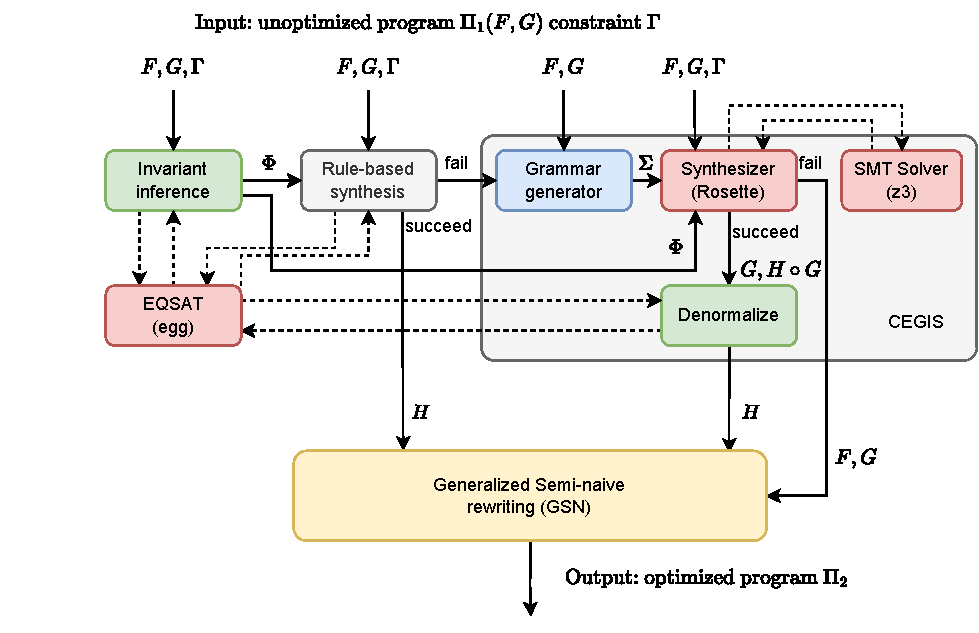
\includegraphics[width=\linewidth]{fgh-optimizer-architecture}
  \caption{The architecture of the FGH-optimizer.  The input is the
    unoptimized program $\Pi_1$, consisting of the functions $F, G$ and
    the database constraint $\Gamma$. The output consists of the
    optimized program $\Pi_2$, see Eq.~\eqref{eq:p1:p2}.  Blue boxes are
    described in Section~\ref{subsec:synthesis} and the green boxes in
    Section~\ref{sec:semantic-opt}.  The yellow box
    (generalized semi-naive optimization) is described in
    Section~\ref{subsec:simple:examples}.  The red boxes represent
    three state-of-the-art systems: Rosette is a \cegis\ system~\cite{DBLP:conf/asplos/Solar-LezamaTBSS06,DBLP:conf/tacas/TorlakJ07,DBLP:conf/oopsla/TorlakB13}, \zzz\ is
    an SMT solver~\cite{10.1007/978-3-540-78800-3_24}, and EGG is an \eqsat\ system~\cite{DBLP:journals/pacmpl/WillseyNWFTP21}.}\label{fig:arch}
\end{figure}


In the rest of the paper we describe our synthesis-based
FGH-optimizer, whose architecture is shown in Fig.~\ref{fig:arch}.  We
optimize one stratum at a time.  We denote by $\Pi_1$ one stratum of
the input program, denote by $X$ its recursive IDBs, by $Y$ its output
IDBs, and by $F,G$ the ICO and the output operator respectively; see
Eq.~\eqref{eq:p1:p2}.  The optimizer also takes as input a database
constraint, $\Gamma$.  The optimizer starts by inferring the loop
invariant $\Phi$; this is discussed in Sec.~\ref{sec:semantic-opt}.
Next, the optimizer needs to find $H$ such that
$\Gamma \wedge \Phi \models \left(G(F(X)) = H(G(X))\right)$.  To
reduce clutter we will often abbreviate this to
$\Gamma \models \left(G(F(X)) = H(G(X))\right)$, assuming that
$\Gamma$ incorporates $\Phi$.  The optimizer makes two attempts at
synthesizing $H$: it first tries using a simpler rule-based
synthesizer, and, if that fails, then it tries the state-of-the-art
Counterexample-Guided Inductive Synthesis (\cegis).  This is described
in Sec.~\ref{subsec:synthesis}.  Finally, $H$ (or the original program
if the FGH-optimization failed) is further transformed using
generalized semi-naive optimization, as we already described in
Sec.~\ref{subsec:simple:examples}.  Notice that stratification ensures
that no interpreted functions are applied to the IDBs $X$; they can
still be applied to the EDBs, or occur in predicates.

The FGH-optimization is an instance of {\em query rewriting using
  views}~\cite{DBLP:journals/vldb/Halevy01,DBLP:conf/sigmod/GoldsteinL01}.
Denoting by $Q \defeq G(F(X))$ and $V \defeq G(X)$, one has to rewrite
the query $Q$ using the view(s) $V$, in other words $Q = H(V)$.  This
is a {\em total} rewriting, in the sense that $H$ may no longer 
refer to the IDBs $X$.  This problem is NP-complete for UCQs with
set semantics~\cite{DBLP:conf/pods/LevyMSS95}, in NP for UCQs with bag
semantics\footnote{This follows from the fact that, under bag semantics, two UCQ queries are
  equivalent iff they are
  isomorphic.~\cite{DBLP:conf/icdt/Green09,DBLP:journals/pvldb/WangHSHL20}.},
and undecidable for realistic SQL queries that include aggregates and
arithmetic~\cite{DBLP:conf/sigmod/GoldsteinL01}.
%
Systems that support query rewriting using views are rule-based, and
apply a set of hand crafted, predefined patterns; our first attempt to
synthesize $H$ is also rule-based.  Such synthesizers usually cannot take advantage
of database constraints, but we will show in
Sec.~\ref{sec:semantic-opt} how to exploit the constraint $\Gamma$ in
the rule-based synthesizer.  However, rule-based rewriting explores a
limited space, which is insufficient for many FGH-optimizations.
In a seminal paper~\cite{DBLP:conf/asplos/Solar-LezamaTBSS06}
Solar{-}Lezama proposed an alternative to rule-based transformation,
called {\em Counterexample-Guided Inductive Synthesis}, \cegis: the
synthesizer produces potentially incorrect candidates, and an SMT
solver verifies their correctness.  In the FGH-optimizer we use a
program synthesizer, Rosette~\cite{DBLP:conf/oopsla/TorlakB13}, to synthesize $H$.

At a conceptual level, program synthesis has two abstract steps: {\em
  generate} $H$, and {\em verify} $G(F(X))=H(G(X))$.  While the
verifier is not used explicitly, it is used implicitly in the
synthesizer, and we describe it in Sec.~\ref{sec:verification}.  Then we
describe the synthesizer in Sec.~\ref{subsec:synthesis}.


% Our optimizer also uses three state of the art tools
% from verification and programming languages: \zzz\ for model checking,
% Rosette for program synthesis, and EGG for equality saturation.  We
% describe them in sections~\ref{sec:verification},
% ~\ref{subsec:synthesis}, and \ref{?????} respectively.


% Any query optimizer can be seen as a theorem prover, capable of
% proving the equivalence of its input and output. From this perspective,
% the rewrite rules in traditional optimizers can be seen as
% {\em axioms}, and the chain of program transformations done by the optimizer
% following these axioms is a calculational proof of equivalence.
% The optimizer's ability to explore alternatives translates to
% its ability to prove programs equal.
% Following this line of thinking, we first demonstrate how to
% {\em verify} the FGH-rule holds. That is, given $F, G$ and $H$,
% we verify $\forall X . G(F(X)) = H(G(X))$.
% Then, building on this verification procedure, we {\em synthesize}
% the function $H$ given $G$ and $F$.


%%% Local Variables:
%%% mode: latex
%%% TeX-master: "main"
%%% End:

\section{Verification}
\label{sec:verification}

\update{
%
  We introduced the FGH-rule in Sec.~\ref{sec:fgh} and showed several
  examples.  In order to apply the rule, one needs to check the
  identity~\eqref{eq:fgh}, $F(G(X))=G(H(X))$. In this section we
  describe how we verify this identity.
%
}
%
This step is implicit in both boxes {\em Rule-based Synthesis} and
\cegis\ in Fig~\ref{fig:arch}.
%
\update{
%
  The identity can be checked in one of two ways: by applying a
  predefined set of identity rules (as currently done by most query
  optimizers), or by using an SMT solver.
%
}

\subsection{Rule-based  Test}\label{sec:axiomatic-rewrite}
% This test consists of first normalizing both expressions, then
% checking for isomorphism.  We describe the rule-based test assuming
% there is no database constraint $\Gamma$: the extension to $\Gamma$
% can be done using a \eqsat\ system, discussed in
% Sec.~\ref{sec:semantic-opt}.


% to handle interpreted functions.
% To simplify implementation, we preprocess the input
%  Datalog program by mapping all semirings in the program to
% the semiring used in $G$.
% For example, the boolean semiring in $CC_{1}$ is mapped to
% the Tropical semiring as shown in Figure~\ref{fig:cc1:semiring}.
% Unifying to a single semiring saves us from enumerating
% tedious axioms describing how different semirings interact
% with each other, and also simplifies the encoding to SMT
% expressions.
%
Let $P_{1} = G(F(X))$, $P_{2} = H(G(X))$.  To check $P_1=P_2$, the
{\em rule-based test} first normalizes both expressions into a
sum-sum-product expression (Eq.~\eqref{eq:sum:sum:product})
via the semiring axioms, then checks if the expressions are isomorphic:
if yes, then $P_{1} = P_{2}$, otherwise we assume $P_{1}\neq P_{2}$.
The treatment of  a constraint $\Gamma$ will be discussed in Sec.~\ref{sec:semantic-opt}.
This test can be visualized as follows:
%
\begin{align}
  P_{1} \xrightarrow[]{\text{axioms}} \text{normalize}(P_{1})
  \simeq
  \text{normalize}(P_{2}) \xleftarrow[]{\text{axioms}} P_{2}
\label{eq:equality:isomorphism}
\end{align}
%
where $\simeq$ denotes isomorphism.  The Rule-based test is sound.
%i.e., there are no false positives.
When both $P_1, P_2$ are over the
$\N^\infty$ semiring and have no interpreted functions then it
is also
complete~\cite{DBLP:conf/icdt/Green09,DBLP:journals/pvldb/WangHSHL20}.
%
This simple test motivates the need for a complete set of axioms that
allows any semiring expression to be normalized.  The axioms include
standard semiring axioms, and axioms about summations and free
variables \texttt{fv}.  For example, in order to
prove $CC_1 = CC_2$ in Example~\ref{ex:fgh:cc} (with
semiring notation in Figure~\ref{fig:cc1:semiring}) one needs
all three axioms below:
%
\begin{align}
  \bigoplus_x \bigoplus_y \left(\cdots\right) = \ &  \bigoplus_{x,y}\left( \cdots \right)  \label{eq:axiom:plus:plus} \\
  A \otimes \bigoplus_{x} B = \ & \bigoplus_{x} A \otimes B \text{ when } x \not \in \texttt{fv}(A) \label{eq:axiom:pullmul}\\
  \bigoplus_x \left(A(x) \otimes [x=y]\right) = \ & A(y)  \label{eq:axiom:plus:equal}
\end{align}
%

%
%
%
%
% \begin{example} We illustrate how to check of the FGH-rule in
%   Example~\ref{ex:fgh:cc}.  The two expressions $P_1, P_2$ were denote
%   $CC_1, CC_2$ and are shown in Figures~\ref{fig:cc1}
%   and~\ref{fig:cc2}.  We first de-sugar them and write them as
%   semiring expressions, as shown in Figure~\ref{fig:cc1:semiring}.
%   Recall that the cast operator $[-]_\infty^0$ maps the Boolean values
%   $0,1$ to the tropical values $\infty, 0$. We normalize both
%   expressions, using semiring axioms such as:
% %
%   \begin{align}
%     \bigoplus_x \bigoplus_y \left(\cdots\right) = &  \bigoplus_{x,y}\left( \cdots \right)  \label{eq:axiom:plus:plus} \\
%     A \otimes \bigoplus_{x} B = & \bigoplus_{x} A \otimes B \text{ when } x \not \in \texttt{fv}(A) \label{eq:axiom:pullmul}\\
%     \bigoplus_x \left(A(x) \otimes [x=y]\right) = & A(y)  \label{eq:axiom:plus:equal}
%   \end{align}
% %
%   We have designed a complete set of semiring axioms for converting
%   into a sum-sum-product expression, similar to axioms found
%   elsewhere,
%   e.g., \cite{DBLP:journals/pvldb/ChuMRCS18,DBLP:journals/pvldb/WangHSHL20}.
%   After normalization, we obtain:
% %
%   \begin{align*}
%     \text{normalize}(CC_{1}[x]) & = L[x] \oplus \bigoplus_{y,z} L[y] \otimes \totrop{E(x,z)} \otimes [TC(z,y)]_{\infty}^{0}\\
%                                 & \simeq \text{normalize}(CC_{2}[x])
%   \end{align*}
% %
%   proving their equivalence.
% %   Each rewrite step during normalization applies some semiring axioms,
% %   for example: where $\texttt{fv}(A)$ is the set of free variables in
% %   $A$.  We use standard semiring identities like the commutativity and
% %   associativity of $\oplus$ and $\otimes$ in the normalization step.
% %   We omit the exhaustive list of axioms, and refer the reader
% %   to~\cite{??} for details.
% \end{example}
%

% In some cases this mapping is lossless;
% for example boolean disjuction $x \vee y$ can be mapped
% via inclusion-exclusion to $[x] + [y] - [x] \times [y]$,
% where $[\cdot]$ casts \texttt{true} to $1$ and
% \texttt{false} to $0$.
% In other cases this mapping is lossy.
% For example we map $\min(x,y)$ to $x+y$,
% however $\min(x,x) = x$ but $x+x \neq x$.
% In general, mapping to the sum-product semiring is always
% sound:
% \begin{theorem}[Equality over $(\N, +, \times, 0, 1)$ is canonical]\label{th:soundness}
%   $[e_{1}]_{\N} = [e_{2}]_{\N} \Rightarrow e_{1} = e_{2}$,
%   where $e_{1}$ and $e_{2}$ are over the same semiring, and
%   $[\cdot]_{\N}$ maps an expression in any semiring to the sum-product semiring.
% \end{theorem}
% We note that it is possible, albeit tedious, to skip this
% processing step and apply axioms specific to each semiring,
% and to directly encode each semiring in SMT formulas.
% An industrial-strength optimizer may opt to do so to achieve
% better coverage.
\begin{figure}
% \fcolorbox{black}{light-gray}{\parbox{0.2\textwidth}{
  \begin{align*}
    CC_{1}[x] & = \bigoplus_{y} L[y] \otimes \big([x=y]_{\infty}^{0} \oplus \bigoplus_{z} [E(x,z)]_{\infty}^{0} \otimes [TC(z,y)]_{\infty}^{0}\big) \\
    CC_{2}[x] & = L[x] \oplus \bigoplus_{y} \big( \bigoplus_{y'} L[y'] \otimes [TC(y,y')]_{\infty}^{0}\big) \otimes [E(x,y)]_{\infty}^{0}
  \end{align*}
% }}
  \caption{$CC_{1}$ and $CC_{2}$ in semiring notation; their normal
    forms are isomorphic.}
  \label{fig:cc1:semiring}
\end{figure}
% \begin{figure}
% \fcolorbox{black}{light-gray}{\parbox{0.2\textwidth}{
% \footnotesize
%   \begin{align*}
%     CC_{2}[x] \defeq L[x] \oplus \bigoplus_{y} 1_{E(x,y)} \otimes \bigoplus_{y'} L[y'] \otimes 1_{TC(y,y')}
%   \end{align*}
% }}
%   \caption{$CC_{2}$ in semiring notation.}
%   \label{fig:cc2:semiring}
% \end{figure}

\subsection{SMT Test} \label{subsubsec:smt:test} When the
expressions $P_1, P_2$ are over a semiring other than $\N^\infty$, or
they contain interpreted functions, then the rule-based test is
insufficient and we use an SMT solver for our verifier.
We still normalize the
expressions using our axioms, because today's solvers cannot reason
about bound/free variables (as needed in
axioms~\eqref{eq:axiom:plus:plus}-\eqref{eq:axiom:plus:equal}).  The
{\em SMT test} is captured by the following figure:
% After we normalize both expressions
% $P_{1}$ and $P_{2}$, if the isomorphism test fails, then we check
% their equivalence using an SMT solver: $\Gamma \models (P_1=P_2)$.
% More precisely, we ask the solver to find a {\em counterexample}, i.e.,
% IDB and EDB instances for which
% $\Gamma \wedge (\text{normalize}(P_1)\neq \text{normalize}(P_2))$.  If
% the solver fails, i.e., returns \textsf{UNSAT}, then we know that
% $P_1 = P_2$.  The following figure captures this process:
%
%
% If the equality is
% valid, $P_{1}$ and $P_{2}$ are equivalent; otherwise they are not, and
% the solver will return a {\em counterexample} input to $P_{1}$ and
% $P_{2}$ on which they evaluate to different results.  We illustrate
% this process as follows:
\begin{align}
  P_{1} \xrightarrow[]{\text{axioms}} \text{normalize}(P_{1})
  \xleftrightarrow{\text{SMT}} &
  \text{normalize}(P_{2}) \xleftarrow[]{\text{axioms}} P_{2} \label{eq:equality:smt}
\end{align}

\begin{ex}[APSP100]\label{ex:sssp100}
  Consider a labeled graph $E$ where $E[x,y]$ represents the cost of
  the edge $x,y$.  The following query over $\trop$
  computes the all-pairs shortest
  path up to length of 100:
%
{
  \begin{align}
    D[x,y] \cd & \texttt{if } x=y \texttt{ then } 0 \texttt{ else } \min_{z} \left(D[x,z] +E[z,y]\right) \nonumber \\
    Q[x,y] \cd & \min(D[x,y],100)  \label{eq:apss:opt}
  \end{align}
}
%
  % The first rule is not {\em safe}, because $x$ does not occur in
  % relational atom; one can convert it to a safe rule by restricting
  % $x$ to range over the set of nodes in the graph, but we omit that in
  % order to reduce clutter.  The second rule is both recursive {\em
  %   and} contains an aggregate operator, $\min$.  If one were to
  % represent it in standard Datalog, it would be something like this:
%
  % \begin{align*}
  %   D(x,y,\min(v+c)) \cd & D(x,z,v),E(z,y,c)
  % \end{align*}
%
  % In standard  Datalog rules with aggregates are not monotone.  In
  % order to add such rules to Datalog, prior
  % work~\cite{DBLP:conf/pods/GangulyGZ91,DBLP:journals/tkde/SeoGL15}
  % has re-defined the semantics of the $\min$ operator, whenever it
  % occurs in the head of a recursive rule.  Instead, in $\name$ our
  % approach is to use a standard semantics, by generalizing from the
  % Boolean semiring to an arbitrary ordered semiring.  The
  % program~\eqref{eq:apss:opt} is interpreted over the tropical
  % semiring $\trop = (\N \cup \set{\infty},\min,+,\infty,0)$.  The
  % program is monotone and has a unique least fixpoint.
  The program is inefficient because it first computes the full path
  length, only to cap it later to 100.  By using the FGH-rule we get:
%
{
  \begin{align}
    Q[x,y] \cd & \texttt{if } x=y \texttt{ then } 0 \texttt{ else } \min\left(\min_{z} \left(Q[x,z]+E[z,y]\right),100\right) \label{eq:apss:opt:opt}
  \end{align}
}
%
We show how to verify
that~\eqref{eq:apss:opt:opt} is equivalent to~\eqref{eq:apss:opt}.
Denote by $P_1 \defeq G(F(D))$ and $P_2 \defeq H(G(D))$ (where $F,G,H$
are the obvious functions in the two programs defining $Q$).  After we
de-sugar, convert to semiring expressions, and normalize,
they become:
%
{
\begin{alignat*}{2}
  P_{1}[x,y] & =  \left(0 \otimes \totrop{x=y}\right) \oplus \left(\bigoplus_{z} D[x,z] \otimes E[z,y]\right) && \oplus 100 \\
  P_{2}[x,y] % & = 0 \otimes \totrop{x=y} \oplus 100 \oplus \bigoplus_{z} (D[x,z] \oplus 100) \otimes E[z,y] \\
             % & = 0 \otimes \totrop{x=y} \oplus 100 \oplus \bigoplus_{z} D[x,z] \otimes E[z,y] \\
             % & \hskip 59pt \oplus \bigoplus_{z} 100 \otimes E[z,y] \\
%              & = 100 \oplus 0 \otimes \totrop{x=y} \oplus \bigoplus_{z} D[x,z] \otimes E[z,y] \\
%              & \hskip 25pt \oplus 100 \otimes \bigoplus_{z} E[z,y] \\
             & = \left(0 \otimes \totrop{x=y}\right) \oplus \left(\bigoplus_{z} D[x,z] \otimes E[z,y]\right) && \oplus \left(100 \otimes\bigoplus_{z} E[z,y]\right) \\
             &&& \oplus 100
\end{alignat*}
}
%
In the normalized expressions we push the summations past the joins,
i.e., we apply rule~\eqref{eq:axiom:pullmul} from right to left, thus
we write $100 \otimes \bigoplus (\cdots)$ instead of
$\bigoplus (100 \otimes \cdots)$: we give the rationale below.  At
this point, the normalized $P_{1}$ and $P_{2}$ are not isomorphic, yet
they are equivalent if they are interpreted in $\trop$.
We explain below in detail how the solver can check that.
In this particular semiring,
the
identity
$
  100 = \left(100 \otimes \bigoplus_{z} E[z,y]\right)  \oplus 100
$
holds since it becomes
$
100 = \min(100 + \min_{z} E[z,y],100)
$
with $E[z,y] \geq 0$,
once we replace the uninterpreted operators
$\oplus, \otimes$ with $\min, +$.
%
% As we explain below, an SMT solver can prove this identity given that
% $E[z,y] \geq 0$.  More precisely, using the \zzz\ solver, we discover
% that the following is \textsf{UNSAT}:
% \[
% x \geq 0 \wedge 100 \neq \min(100 + x, 100)
% \]
% from which we can conclude
% $\forall x . x \geq 0 \Rightarrow 100 = \min(100, 100 + x)$.
\end{ex}


{\bf Implementation} We describe how we implemented the SMT test
$\Gamma \models P_1 = P_2$ using a solver, now also taking
the database constraint $\Gamma$ into account, where
$P_1, P_2$ are the expressions $G\circ F$
and $H \circ G$. We used the \zzz\ solver~\cite{10.1007/978-3-540-78800-3_24}, but our
discussion applies to other solvers as well. We need to normalize
$P_1, P_2$ before using the solver, because solvers require all axioms
to be expressed in First Order Logic. They cannot encode the
axioms~\eqref{eq:axiom:plus:plus}-\eqref{eq:axiom:plus:equal}, because
they are referring to free variables, which is a
meta-logical condition not expressible in First Order Logic.
Once normalized, we encode the equality as a first-order logic
formula, and assert its negation, asking the solver to check if
$\Gamma \wedge \left(P_1 \neq P_2\right)$ is satisfiable.  The solver
returns $\textsf{UNSAT}$, a counterexample, or
$\textsf{UNKNOWN}$.  $\textsf{UNSAT}$ means the
identity holds.  When it returns a counterexample, then the identity
fails, and the counterexample is given as input to the synthesizer
(Sec.~\ref{subsec:synthesis}).  $\textsf{UNKNOWN}$ means that it could
neither prove nor disprove the equivalence and we
assume $P_1 \neq P_2$.  For the theory of reals with $+, *$, despite its
decidability,  \zzz\ often timed out in our experiments.
We therefore used the theory of integers, and
\zzz\ never timed out or returned $\textsf{UNKNOWN}$ in our experiments.



We encode every $\bm S$-relation
$R(x_1, \dots, x_n)$ as an uninterpreted function
$R : \N \times \cdots \times \N \rightarrow \bm S$, where $\bm S$ is
the {\em interpreted} semiring, i.e., $\B$, $\trop$, $\N^\infty$, etc.
We represent natural numbers as
integers with nonnegativity assertions, and represent
the sets $\N^\infty, \N_\bot, \R_\bot$ as union types.
Operators supported by the solver, like $+, *, \min, -$,
are entered unchanged; we treat other operators
as uninterpreted functions.  Unbounded aggregation, like
$\bigoplus_{x} e(x)$, poses a challenge:  there is no
such  operation in any SMT theory.
%%% One may attempt to unfold
%%% the aggregate over some bounded values of $x$, say replace
%%% $\min_{x} e(x)$ with $\min(e(0), \dots, e(20))$, but this approach is
%%% unsound.
Here we use the fact that $P_1$ and $P_2$ are normalized
sum-sum-product~expressions:
%
\begin{align*}
P_1 = & \left(\bigoplus_{x_1} e_1\right) \oplus \left(\bigoplus_{x_2}  e_2\right) \oplus \cdots
&
P_2 = & \left(\bigoplus_{x_1'} e_1'\right) \oplus \left(\bigoplus_{x_2'} e_2'\right) \oplus \cdots
\end{align*}
%
Assume first that each $x_i$ is a single variable. We
ensure that all the variables $x_1, x_2, \ldots$ in $P_1$ are
distinct, by renaming them if necessary.  Next, we replace each
expression $\bigoplus_{x_i} e_i$ with $u(x_i,e_i)$ where $u$ is an
uninterpreted function.  Finally, we ask the solver to check
%
\begin{align}
\Gamma \models \left(u(x_1,e_1) \oplus u(x_2,e_2) \oplus \cdots =  u(x_1',e_1') \oplus u(x_2',e_2') \oplus \cdots\right)
\nonumber
% \label{eq:ui:uj}
\end{align}
%
This procedure is sound, because if the identity $u(x,e) = u(x',e')$
holds, then $x=x'$ (they are the same variable) and $e=e'$, which
means that $\bigoplus_x e = \bigoplus_{x'} e'$.  Moreover,
when synthesizing $P_2$, we will
ensure that the generator includes the variables $x_1, x_2, \ldots$
present in $P_1$ to achieve a limited form of completeness,
see
Sec.~\ref{subsec:synthesis}. Finally, if a
summation is over multiple variables, we simply nest the uninterpreted
function, i.e., write $\bigoplus_{x,y} e$ as $u(x,u(y,e))$.

\begin{ex}  We now finish Example~\ref{ex:sssp100}.
After introducing the
  uninterpreted functions described above, we obtain:
%
  \begin{align*}
    P_1 = & \min(0+w(x,y), u(z,D[x,z]+E[z,y]), 100) \\
    P_2 = & \min(0+w(x,y), u(z,D[x,z]+E[z,y]), 100+u(z,E[z,y]), 100)
  \end{align*}
  where $w(x,y)$ is an uninterpreted function representing
  $[x=y]_\infty^0$, and $u$ is our uninterpreted function encoding
  summation.  The solver proves that the two expressions are equal,
  given that $w \geq 0$ and $u \geq 0$.  Notice that it was critical
  to factorize the term 100: had we not done that, then the expression
  $100+u(z,E[z,y])$ would be $u(z,100 + E[z,y])$ and the identity
  $P_1=P_2$ no longer holds.
\end{ex}

\required{
%
  {\bf Discussion} Readers unfamiliar with First Order Logic may be
  puzzled by our statement that the identity $u(x,e)=u(x',e')$ holds
  iff $x=x'$ and $e = e'$.  In order to explain this, it helps to
  first review the basic definitions of validity and satisfiability in
  logic.  A statement is ``valid'' if it is true for all
  interpretations of its uninterpreted symbols.  For example, the
  equality $f(x)+y=y+f(x)$ is valid over integers, because it holds
  for all function $f$ and all values of $x$ and $y$.  A statement is
  ``satisfiable'' if there exists interpretations of its uninterpreted
  symbols that make the statement true.  A statement is valid iff its
  negation is not satisfiable.  In our case, the statement
  $u(x,e)=u(x',e')$ is valid if the equality is true for all possible
  interpretations of $u, x, x'$.  For example, suppose we asked the
  solver to check whether $u(x,2(x+1)) = u(y,2y+2)$ is valid.  To
  answer this question, we negate the statement and ask the \zzz\
  solver whether the negation is satisfiable:
  $u(x,2(x+1))\neq u(y,2y+2)$.  One can easily satisfy this with pen
  and paper, e.g.,  $x=1, y=2, u(a,b)=a+b$, then $u(x,2(x+1))=5$,
  $u(y,2y+2)=8$.  \zzz\ also answers ``yes'', and provides the
  following example for the inequality\footnote{Please refer to the
    documentation of \zzz\ for how models for uninterpreted functions
    are constructed.}:
  \[x=0, y=38, u(a,b)= \text{if } a=38\wedge b=78 \text{ then } 6 \text{ else } 4\]
  Therefore, the identity $u(x,2(x+1)) = u(y,2y+2)$ is not valid.  In
  contrast, suppose we asked the solver whether
  $u(x,2(x+1)) = u(x,2x+2)$ is valid.  Its negation is
  $u(x,2(x+1)) \neq u(x,2x+2)$, and \zzz\ returns $\textsf{UNSAT}$,
  which means that the identity is valid.  In general, the identity
  $u(x,e)=u(x',e')$ is valid iff $x=x'$ and $e=e'$.
%
}


% \reinhard{uniform notation: $p_1$ and $p_2$ vs. $P_1$ and $P_2$?}
% \dan{done; hope  i didn't missed anything}

% This encoding of aggregates is complete
% in the following sense:
% %
% \begin{theorem}[Encoding $\bigoplus$ with uninterpreted functions]
%   $\bigoplus_{x} e = \bigoplus_{x'} e' \Leftrightarrow f_{\bigoplus}(x, e) = f_{\bigoplus}(x',e')$
%   where $\bigoplus_{x} e$ and $\bigoplus_{x'} e'$ are in normal form.
% \end{theorem}
% %
% The following shows the SMT encoding of $Q_{1}$ and $Q_{2}$:
% \begin{align*}
%   Q_{1} & : \min(100, 0 + \totrop{x=y}, f_{\min}(z, f_{D}(x,z) + f_{E}[z,y])) \\
%   Q_{2} & : \min(100, 0 + \totrop{x=y}, f_{\min}(z, f_{D}(x,z) + f_{E}[z,y]), \\
%         & \hskip 26pt 100 + f_{\min}(z, f_{E}[z,y]))
% \end{align*}

%%% \subsubsection{Discussion} In summary, our verifier checks $p_1 = p_2$
%%% by first normalizing both expressions, checking for isomorphism,
%%% \eqref{eq:equality:isomorphism} and, if that fails, then using the
%%% \zzz\ solver to check their equivalence, \eqref{eq:equality:smt}.  The
%%% reader may wonder why we don't bypass normalization altogether and
%%% perform the entire verification pipeline in the solver.  The reason is
%%% that the solver requires all axioms to be expressed in First Order
%%% Logic, while some crucial axioms needed for identities of
%%% sum-sum-product expressions require checking for free variables, as in
%%% example~\eqref{eq:axiom:pullmul}, which is a meta-logical condition,
%%% and not expressible in First Order Logic.  In other words, we are
%%% extending the solver with specialized knowledge about the semiring.

%
% Moreover, other axioms
% expressible in FOL usually require quantification and can easily make
% SMT-solving undecidable or intractable. \dan{I don't understand the
%   last sentence}

% In summary, the verification process first normalizes the pair of expressions
% to be checked.
% If the normal forms are isomorphic, the expressions are equivalent and verification succeeds.
% Otherwise, we encode the expressions in an SMT formula that asserts their equivalence,
% then checks the validity of this formula with an SMT solver.
% The entire pipeline looks like the following:

%%% Local Variables:
%%% mode: latex
%%% TeX-master: "main"
%%% End:

\section{Synthesis}

\label{subsec:synthesis}

%%% \dan{currently: 1.5 pages.  GOAL: 1 PAGE.  Reinhard: the section is
%%%   complete, but can use lots of polishing, feel free to edit it.}

\update{
%
We have seen in Sec.~\ref{sec:verification} how to use an SMT solver
to check the identity $G(F(X))=H(G(X))$.
%
}
%
We are now ready to discuss the core of the FGH-optimizer: given 
the query expressions $F, G$, find $H$ such that the
identity $G(F(X)) = H(G(X))$ holds; recall that we denote these
expressions by $P_1, P_2$. As for verification, this can be done by
using only rewriting, or using program synthesis with an SMT solver.
We are also given a database constraint $\Gamma$, and we assume that
 we have already added to it the loop invariant $\Phi$.


\subsection{Rule-based Synthesis}
\label{subsec:rule:based:synthesis}

The optimizer first attempts to synthesize $H$ using rule-based
rewriting.  This process is akin to our initial verifier that relies
only on normalization and isomorphism checking.
%
\begin{align}
  P_{1} \xrightarrow[]{\text{axioms}} \text{normalize}(P_{1}) \xrightarrow[]{\text{axioms}} P_{2}
  \label{eq:synthesis:isomorphism}
\end{align}
%
There is no obvious way to ``denormalize'' an expression, since many
expressions share the same normal form.  We used for this purpose
an equality saturation system (\eqsat), also used for multiple tasks
of the FGH-optimizer, see Fig~\ref{fig:arch}.  We describe \eqsat\ in Sec.~\ref{sec:semantic-opt}.
% One possibility is to apply one of the query rewriting using views
% algorithms, like MiniCon~\cite{DBLP:journals/vldb/PottingerH01} or
% pattern-matching as used in SQL
% Server~\cite{DBLP:conf/sigmod/GoldsteinL01}.  Instead, we use for
% this purpose an equality saturation system, described in
% Sec.~\ref{sec:semantic-opt}.

% \reinhard{Can we give a short justification for our decision to use
% an equality saturation system?}


%%% Instead, we chose to use for this purpose a state of the art {\em
%%%   equality saturation} system (\eqsat) developed in the programming
%%% language community, called
%%% EGG~\cite{DBLP:journals/pacmpl/WillseyNWFTP21}.  Using an open source
%%% \eqsat\ system simplifies considerably the development of our
%%% optimizer, but, conceptually, it does not bring anything new to {\em
%%%   this task} over what was previously known in the literature, so we
%%% delay its description to Sec.~\ref{sec:semantic-opt}.

% A brute-force approach is
% to rewrite the input $P_{1}'$ to as many equivalent expressions as
% possible, and then look for an expression of the form $H(G(X))$ among
% the results.  This naive idea is implemented efficiently by an
% innovation in programming languages dubbed {\em equality saturation}
% (\eqsat).



\subsection{Counterexample-based Synthesis}

The rule-based synthesis~\eqref{eq:synthesis:isomorphism} explores
only correct rewritings $P_2$, but its space is limited by the
hand-written axioms. The alternative approach, pioneered in the
programming language
community~\cite{DBLP:conf/asplos/Solar-LezamaTBSS06}, is to synthesize
candidate programs $P_2$ from a much larger space, then using an SMT
solver to verify their correctness.  This technique, called
Counterexample-Guided Inductive Synthesis, or \cegis, can find
rewritings $P_2$ even in the presence of interpreted functions,
because it exploits the theory of the underlying domain.  As a first
attempt it can be described as follows (we will revise it below):
%
\begin{align}
  P_{1} \xrightarrow[]{\text{axioms}} \text{normalize}(P_{1}) \xrightarrow[]{\cegis} P_{2}
  \label{eq:synthesis:cegis}
\end{align}
%

\subsubsection{Brief Overview of \cegis} We give a brief overview of
the \cegis\ system,
Rosette~\cite{DBLP:conf/tacas/TorlakJ07,DBLP:conf/oopsla/TorlakB13},
that we used in our optimizer.  Understanding its working is
important in order to optimize its usage for FGH-optimization.  The
input to Rosette consists of a {\em specification} and a {\em
  grammar}, and the goal is to synthesize a program defined by the
grammar and that satisfies the specification.
% The \cegis\ algorithm is illustrated by Figure~\ref{fig:cegis}.
The main loop is implemented with a pair of {\em dueling} SMT-solvers,
the {\em generator} and the {\em checker}.  In our setting, the inputs
are the query $P_1$, the database constraint $\Gamma$, and a small
grammar $\Sigma$ (described below).  \update{The specification is
  $\Gamma \models (P_1 = P_2)$, where $P_2$ is defined by the grammar
  $\Sigma$.}  The generator generates syntactically correct programs
$P_2$, and the verifier checks $\Gamma \models (P_1 = P_2)$.  In the
most naive attempt, the generator could blindly generate candidates
$P_2, P_2', P_2'', \ldots$, until one is found that the verifier
accepts.  This is hopelessly inefficient.  The first optimization in
\cegis\ is that the verifier returns a small counterexample database
instance $D$ for each unsuccessful candidate $P_2$, i.e.,
$P_1(D)\neq P_2(D)$.  When considering a new candidate $P_2$, the
generator checks that $P_1(D_i) = P_2(D_i)$ holds for all previous
counterexamples $D_1, D_2, \ldots$, by simply evaluating the queries
$P_1,P_2$ on the small instance $D_i$.  This significantly reduces the
search space of the generator.

\cegis\
applies a second optimization, where it uses the SMT solver itself to
generate the next candidate $P_2$, as follows.  It requires a fixed
recursion depth for the grammar $\Sigma$; in other words we can assume
w.l.o.g. that $\Sigma$ is non-recursive.  Then it associates a
symbolic Boolean variable $b_1, b_2, \ldots$ to each choice of the
grammar.  The grammar $\Sigma$ can be viewed now as a BDD (binary
decision diagram) where each node is labeled by a choice variable
$b_j$, and each leaf by a completely specified program $P_2$.  The
search space of the generator is now completely defined by the choice
variables $b_j$, and Rosette uses the SMT solver to generate values
for these Boolean variables such that the corresponding program $P_2$
satisfies $P_1(D_i) = P_2(D_i)$, for all counterexample instances
$D_i$.  This significantly speeds up the choice of the next candidate
$P_2$.


% The \eqsat-based optimization of pure $\name$ can be
% understood in parallel to the normalization-based verification
% process: both rely on axiomatic rewrites of the input expressions.
% Similarly, our optimizer for $\name$ with interpreted functions
% builds on the solver-aided verification procedure.
% In verifying the FGH-rule we start from the expressions
% $G(F(X))$ and $H(G(X))$ and ``meet in the middle'';
% the optimization problem requires us to start from the initial
% program $G(F(X))$ and arrive at the optimized program $H(G(X))$.
% We summarize our query synthesis pipeline as follows:
% \[
%   G(F(X)) \xrightarrow[]{\text{axioms}} \text{normalize}(P_{1})
%   \xrightarrow[]{\cegis}
%   P_{2}' \xrightarrow[]{\eqsat} H(G(X))
% \]
% We first normalize the input program $G(F(X))$
% to $\text{normalize}(P_{1})$ by applying semiring axioms.
% Then we leverage counterexample-guided inductive synthesis (\cegis),
% a novel technique from programming languages,
% to synthesize $P_{2}'$ such that $ P_{2}' = \text{normalize}(P_{1})$;
% furthermore, $P_{2}'(X)$ must be the normal form of $H(G(X))$ for some $H$.
% Finally, we denormalize $P_{2}'(X)$ into $H(G(X))$ with \eqsat\
% and extract the optimized recursive definition $H$.

% \subsubsection{Query synthesis with \cegis}

% \begin{figure}
%   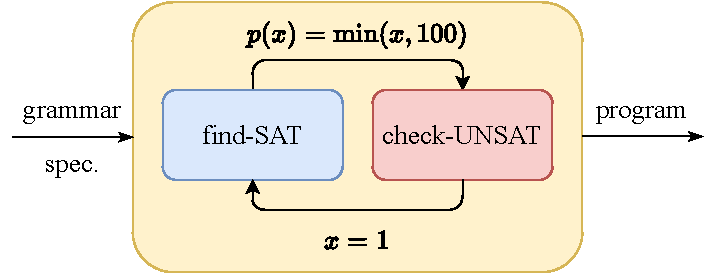
\includegraphics[width=0.8\linewidth]{duel}
%   \caption{Architecture of \cegis.}\label{fig:cegis}
% \end{figure}

% \cegis~takes a grammar $\Gamma$ and a specification $\psi$,
% and outputs a program $p$ drawn from $\Gamma$ that satisfies $\psi$.
% $\psi$ is a first-order formula where the input variables to $p$
% are $\forall$-quantified;
% $\Gamma$ is a conjunction of implications,
% where each implication specifies one alternative in the grammar.


% \begin{example}[Simple \cegis\ Problem]\label{ex:simple:cegis}
%   The following specifies a \cegis\ problem
%   to find a $p$ such that $\forall x . 100 = 100 + p(x)$,
% given the grammar $p(x) \coloneqq 100 + x \mid \min(100, x)$.
%   \begin{gather*}
%     \psi \defeq \forall x . 100 = 100 + p(x)\\
%     \Gamma \defeq (b \Rightarrow p(x) = 100 + x) \wedge (\neg b \Rightarrow p(x) = \min(100, x))
%   \end{gather*}
%   Each pair of $b$ and $\neg b$ correspond to
%   a choice operator ``$\mid$'' in the grammar.
%   Note this is the main step checked by the SMT solver
%   in verifying Example~\ref{ex:sssp100}.
% \end{example}

% The essence of the \cegis\ algorithm is illustrated by Figure~\ref{fig:cegis}.
% The main loop is implemented with a pair of {\em dueling} SMT-solvers,
% one called the {\em generator} (in blue)
% and the other the {\em checker} (in red).
% The generator maintains an initially empty set of counterexamples \textsf{CE}.
% At every iteration of the loop, it draws a program from the grammar that
% satisfies $\psi$ on all existing counterexamples.
% To do so, it solves the following formula:
% $$\Gamma \wedge \bigwedge_{v\in \textsf{CE}} \psi(v)$$
% where $\psi(v)$ means to substitute the quantified variable in $\psi$ with $v$.
% For example, given $\Gamma$ and $\psi$ in Example~\ref{ex:simple:cegis}
% with $\textsf{CE} = \{ 0\}$ the generator solves:
% \begin{gather*}
%   \Gamma \defeq (b \Rightarrow p(x) = 100 + x) \wedge (\neg b \Rightarrow p(x) = \min(100, x)) \\
%   \Gamma \wedge x = 0 \wedge 100 = 100 + p(x)
% \end{gather*}
% This is satisfiable by assigning either \texttt{true} or \texttt{false} to $b$;
% suppose the generator binds $b$ to \texttt{false},
% therefore proposing $p(x) = \min(100, x)$ as a candidate solution.
% It sends this candidate to the checker to verify its correctness against $\psi$.
% Upon receiving a candidate $p$, the checker instantiates $\psi$ with it
% and checks the validity of the resulting formula, by solving its negation:
% \begin{gather*}
%   \text{SAT?}\Big(
%   \neg\big(100 = 100 + p(x) \big)
% \Big)
%   \text{ where } p(x) \defeq \min(100, x)
% \end{gather*}
% This is satisfied when $x=1$, so the candidate $p(x) = \min(100, x)$ is not correct.
% The checker then adds $1$ to \textsf{CE} as feedback
% explaining why the candidate is wrong.
% As this generate-check loop continues,
% the proposed candidate will satisfy $\psi$ on more and more inputs.
% When the checker returns \textsf{UNSAT},
% it has found a correct $p$ and outputs it as the solution.
% On the other hand,
% an \textsf{UNSAT} result from the generator indicates the \cegis\ problem has no solution.
% Indeed, the generator would propose the correct $p$ on the next iteration
% on our example problem, because $b$ must be set to \texttt{true}
% to satisfy $\Gamma \wedge \psi(1)$.
%
% To incorporate \cegis\ into our synthesis pipeline,
% we define the specification to be:
% \[
% \psi \defeq \forall X .  \text{normalize}(P_{1})(X) = p(X)
% \]
% The challenge now is to define the grammar $\Gamma$,
% such that any $p(X)$ drawn from $\Gamma$ can be denormalized into $H(G(X))$
% for some $H$.
% We can design such a grammar by analyzing the possible forms $H(G(X))$ may take.

\subsubsection{Using Rosette} To use Rosette, we need to define the
specification and the grammar. A first attempt is to simply define
some grammar for $H$, with the specification
$\Gamma \models \left(G(F(X)) = H(G(X))\right)$.  This does not work,
since Rosette uses the SMT solver to check the identity: as explained
in Sec.~\ref{subsubsec:smt:test}, modern SMT solvers have limitations
that require us to first normalize $G(F(X))$ and $H(G(X))$ before
checking their equivalence.
Even if we modify Rosette
to normalize $H(G(X))$ during verification,
there is still no obvious way to incorporate normalization
into the program generator driven by the SMT solver.
Instead,
we define a grammar $\Sigma$ for $\text{normalize}(H(G(X)))$ rather
than for $H$, and then specify:
\[
\Gamma \models \text{normalize}(G(F(X))) = \text{normalize}(H(G(X)))
\]
Then, we denormalize the result
returned by Rosette, in order to extract $H$, using the {\em
  denormalization} module in Fig.~\ref{fig:arch}, described in
Sec.~\ref{sec:semantic-opt}.  In summary, our \cegis-approach for
FGH-optimization can be visualized as follows:
%
\begin{align}
  P_{1} \xrightarrow[]{\text{axioms}} \text{normalize}(P_{1}) \xrightarrow[]{\cegis} \text{normalize}(P_{2}) \xrightarrow[]{\text{axioms}} P_{2}
  \label{eq:synthesis:cegis2}
\end{align}
%
The choice of the grammar $\Sigma$ is critical for the FGH-optimizer.
If it is too restricted, then the optimizer will be limited too, if it
is too general, then the optimizer will take a prohibitive amount of
time to explore the entire space.  We briefly describe our design at a
high level.  Recall that $X$ denotes multiple IDBs, and the query
$G(X)$ may also return multiple intermediate relations. In our system
$G(X)$ is restricted to return a single relation, so we will assume
that $Y = G(X)$ is a single IDB.  The expression $G$ is known to us,
and is a sum-sum-product expression, see
Eq.~\eqref{eq:sum:sum:product},
%
\begin{align*}
  G(X) = & G_1(X) \oplus \cdots \oplus G_m(X)
\end{align*}
%
where each $G_i(X)$ is a sum-product expression,
Eq.~\eqref{eq:t:mono}, using the IDBs $X$ and/or the EDBs.

To generate $\texttt{normalize}(H(G(X)))$, \update{we group its
  sum-products by the number of occurrences of $Y$:}
%
\begin{align*}
  \texttt{normalize}(H(Y)) = &  H^{(0)} \oplus H^{(1)}(Y) \oplus
  \cdots \oplus H^{(k_{\max})}(Y)
\end{align*}
%
where $H^{(k)}$ is a sum-sum-product
$H^{(k)} = Q_1 \oplus Q_2 \oplus \cdots$ s.t. each $Q_i$ contains
exactly $k$ occurrences of $Y$, and an arbitrary number of EDBs (it
may not contain the IDBs $X$).  We choose $k_{\max}$ as the largest
number of recursive IDBs $X$ that occur in any rule of the original
program $F(X)$, e.g.,  if the original program was linear, then
$k_{\max} \defeq 1$.  We obtain:
%
{
\begin{align*}
  & \texttt{normalize}(H(G(X))) = \\
  & \ \ \ \   H^{(0)} \oplus \texttt{normalize}(H^{(1)}(G(X))) \oplus \cdots \oplus \texttt{normalize}(H^{(k_{\max})}(G(X)))
\end{align*}
}
%
%
The grammar $\Sigma$ is shown in Fig.~\ref{fig:grammar}.  The start
symbol, $A$, generates a sum matching the expression above.  $A_0$
generates $H^{(0)}$, which is a sum of sum-product terms without any
occurrence of $Y$.  Recall from Sec.~\ref{subsubsec:smt:test} that the
expression $u(z,Q)$ denotes $\bigoplus_z Q$.  $E$ is one of the EDBs,
and $Z$ is a non-terminal for which we define rules
$Z \rightarrow z_1 | z_2 | \cdots | z_m | z_1' | z_2' \cdots$ where
$z_1, \ldots, z_m$ are variables that already occur in
$\texttt{normalize}(G(F(X)))$, and $z_1', z_2', \ldots$ is some fixed
set of fresh variable names. $A_k$ generates
$\texttt{normalize}(H^{(k)}(G(X)))$, which is a sum of sum-products,
each with exactly $k$ occurrence of $Y$.  \update{As stated in
  Fig.~\ref{fig:grammar}, the rules for $A_k$ are incorrect.  For
  example consider $A_1$:}
% The reader may notice that
% the rule for $A_1$ is incorrect as stated.  The reason is that 
the $m$ non-terminals $A_{11}, \ldots, A_{1m}$ \update{should have
  identical derivations, instead of being expanded independently}.
% are independent, but they should instead make precisely the same
% choices.
For example, assume $G = G_1 \oplus G_2$ (thus $m=2$) and we want $H$
to be one of $E_1 \otimes Y$ or $E_2 \otimes Y$ or $E_3 \otimes Y$.
Then, $\texttt{normalize}(H(G(X)))$ can be one of the following three
expressions $E_1\otimes G_1 \oplus E_1 \otimes G_2$ or
$E_2 \otimes G_1 \oplus E_2 \otimes G_2$ or
$E_3 \otimes G_1 \oplus E_3 \otimes G_2$.  However, the grammar
\update{$A_1 \rightarrow A_{11}\oplus A_{12}$} also generates
incorrect expressions $E_1 \otimes G_1 \oplus E_2 \otimes G_2$,
\update{because $A_{11}, A_{12}$ can choose independently the IDB
  $E_1, E_2$, or $E_3$}.  We fix this by exploiting the choice
variables in Rosette: we simply use the same variables in
$A_{11}, A_{12}, \ldots$ ensuring that all these non-terminals make
exactly the same choices.  We note that our current system is
restricted to linear programs, hence $k_{\max}=1$.
% For that reason we do not show $A_k$ for $k \geq 2$ in
% Fig.~\ref{fig:grammar}.

\begin{figure}
\begin{alignat*}{3}
A \rightarrow \ & \parbox{15mm}{\mbox{$A_0 \oplus A_1 \oplus \cdots \oplus A_{k_{\max}},$}} \\
A_0 \rightarrow \ & \parbox{15mm}{\mbox{$Q_0 \mid Q_0 \oplus A_0,\ \ Q_0 \rightarrow \ u(Z,Q_0) \mid Q_0 \otimes Q_0 \mid E(Z,Z,\cdots, Z),$}}\\
A_1\rightarrow \ & \parbox{15mm}{\mbox{$A_{11} \oplus \cdots \oplus A_{1m},\ \ A_2\rightarrow  \  A_{211} \oplus \cdots \oplus A_{2mm}, \ \ A_3 \rightarrow A_{3111}\oplus \cdots$}}\\
A_{1i} \rightarrow \ & Q_{1i} \mid Q_{1i} \oplus A_{1i}, & Q_{1i} \rightarrow \ & u(Z,Q_{1i}) \mid Q_{1i} \otimes Q_0 \mid G_i(X), &i=&1,m\\
A_{2ij} \rightarrow \ & Q_{2ij} \oplus A_{2ij}, & Q_{2ij} \rightarrow \ & u(Z,Q_{2ij}) \mid Q_{1i} \otimes G_j(X), &i,j=&1,m\\
A_{3ij\ell} \rightarrow \ & Q_{3ij\ell} \oplus A_{3ij\ell}, &Q_{3ij\ell} \rightarrow \ & u(Z,Q_{3ij\ell}) \mid Q_{2ij} \otimes G_\ell(X), &i,j,\ell=&1,m
  \end{alignat*}
% }}
\caption{Grammar $\Sigma$ for $\texttt{normalize}(H(G(X)))$, for $k_{\max}=3$.}
  \label{fig:grammar}
\end{figure}




\subsubsection{Discussion}\label{sec:grammar}\ \update{Even though our grammar is
  restricted to $k_{\max}=1$,} it is more complex than
Fig~\ref{fig:grammar}, in order to further reduce the search space.
We use more non-terminals to better control which variables $z$ can be
used where, and we also consider the choice of including entire
subexpressions that occur in the original program $P_1$, since they
are often reused in the optimized program. The synthesizer would
require many trials to find them, had we not included them explicitly.


%
%
% We describe the grammar $\Sigma$ that generates
% $\text{normalize}(P_2)$. In this chapter we only consider $H$ programs
% that are ``linear'' in its argument.  That is, $X$ only appears once
% in the normal form of $H(X)$.  This restriction limits the search
% space and speeds up synthesis, and can still capture the optimizations
% we encounter in practice.  With this restriction, the normal form of
% $H(X)$ has the following form:
% \[\text{normalize}(H(X)): e^{?} \oplus \bigoplus_{\mathbf{V}^{?}} h^{?} \otimes X\]
% where $e^{?}$ is some sum-sum-product expression,
% $\mathbf{V}^{?}$ is a (possibly empty) set of variables,
% and $h^{?}$ is a product of (possibly zero) atoms.
% The superscript $\cdot^{?}$ signifies that the definition of $H$ is not given,
% as we need to synthesize it.
% Suppose $G(X)$ has the normal form:
% \[
%   \text{normalize}(G(X)): \bigoplus_{\mathbf{U}_{1}} g_{1} \oplus \cdots \oplus \bigoplus_{\mathbf{U}_{k}} g_{k}
% \]
% where each $\mathbf{U}_{i}$ is a (possibly empty) set of variables,
% and each $g_{i}$ a product of atoms.
% From the above we can deduce the normal form of $H(G(X))$,
% which must be of the form:
% \[
%   \text{normalize}(H(G(X))):
%   e^{?} \oplus \bigoplus_{\mathbf{U}_{1} \cup \mathbf{V}^{?}} h^{?} \otimes g_{1}
%   \oplus \cdots \oplus
%   \bigoplus_{\mathbf{U}_{k} \cup \mathbf{V}^{?}} h^{?} \otimes g_{k}
% \]
% Using this template as $\Gamma$ ensures any program drawn from it
% can be denormalized to $H(G(X))$.
% We refine the grammar further to prune away programs that have
% no chance of satisfying $\psi$.
% Recall $\psi$ requires the solution $P_{2}'(X)$ to be equal to
% $\text{normalize}(G(F(X)))$.
% Because our SMT encoding treats $\bigoplus$ as uninterpreted,
% $P_{2}'(X)$ must have the same ``shape'' as $\text{normalize}(G(F(X)))$
% at the $\bigoplus$-level.
% That is, given $\text{normalize}(G(F(X)))$ of the form:
% \[
%   \text{normalize}(G(F(X))): \bigoplus_{\mathbf{W}_{1}} f_{1} \oplus \cdots \oplus \bigoplus_{\mathbf{W}_{k}} f_{k}
% \]
% every $\mathbf{U}_{i} \cup \mathbf{V}^{?}$ in $\text{normalize}(H(G(X)))$
% should coincide with a $\mathbf{W}_{j}$ from $\text{normalize}(G(F(X)))$;
% every $\mathbf{W}_{j}$ should coincide with a $\mathbf{U}_{i} \cup \mathbf{V}^{?}$,
% or some aggregated variables in $e^{?}$.
% We therefore define $\Gamma$ as follows:
% \[
%   \Gamma \defeq e^{?} \oplus \bigoplus_{\mathbf{Z}_{1}^{?}} h^{?} \otimes g_{1}
%   \oplus \cdots \oplus
%   \bigoplus_{\mathbf{Z}_{k}^{?}} h^{?} \otimes g_{k}
% \]
% where each $\mathbf{Z}_{i}$ is the unification of $\mathbf{U}_{i} \cup \mathbf{V}^{?}$
% with $\mathbf{W}_{j}$ for some $j$;
% if no such unification exists, there is no $H(G(X))$ that can be equal to $F(G(X))$.
% $e^{?}$ is a sum-sum-product expression that contains exactly the sum-product
% expressions $\bigoplus_{\mathbf{W}_{i}}f_{i}$ that do not participate in the unification.
% Finally, $h^{?}$ is a product of atoms as before;
% we additionally allow an atom in $h^{?}$ to be a comparison like $\leq$.
% After synthesizing $P_{2}'$,
%
% it remains to denormalize $P_{2}'$ into $H(G(X))$.
% But this is precisely the problem of optimizing pure $\name$!
% Therefore we turn to \eqsat\ once again as described in
% Section~\ref{sec:eqsat:fgh} to denormalize $P_{2}$.
% So far, we have used \eqsat\ to implement rewrite-driven optimization;
% \eqsat\ will again play a major role in invariant inference,
% as we discuss in Section~\ref{sec:eqsat:fgh}.


%%% Local Variables:
%%% mode: latex
%%% TeX-master: "main"
%%% End:

\section{Equality Saturation}
\label{sec:semantic-opt}

%%% \dan{I tried to keep this section very short.  If we want to expand
%%%   it, we can get material from the old version which is in the file
%%%   \texttt{semantic-opt.tex} GOAL: KEEP IT 1 PAGE MAX.  Reinhard: feel
%%%   free to edit.}

\begin{figure}
\centering
  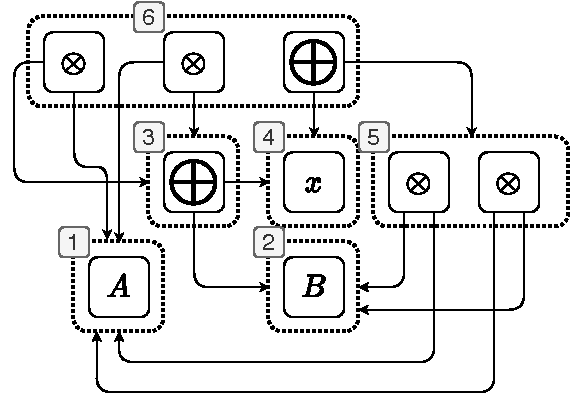
\includegraphics[width=0.45\linewidth]{egraph}
  \caption{Example \egraph.}\label{fig:eqsat}
\end{figure}

Throughout the FGH-optimizer we need to manipulate expressions, apply
rules, and manage equivalent expressions.  This problem is common to
all query optimizers.  Instead of implementing our own expression
manager, 
 we again leverage the equality saturation (\eqsat) system 
 as we did in Chapter~\ref{chapter:spores}.
Specifically, we used
egg~\cite{DBLP:journals/pacmpl/WillseyNWFTP21} to implement the green
boxes in the architecture shown in Fig.~\ref{fig:arch}.

% An \eqsat\ system maintains a data structure called an
% \egraph\ that compactly represents a set of expressions, together with
% an equivalence relation over this set.  Each \egraph\ consists of a set
% of \eclasses, each \eclass\ consists of a set of \enodes, and each
% \enode\ is a function symbol with \eclasses\ as children.
% As a refresher, Figure~\ref{fig:eqsat} shows an \egraph\ representing the two
% expressions in Eq.~\eqref{eq:axiom:pullmul}, their subexpressions, and
% other equivalent expressions.  Each \eclass\ (dotted box) represents a class of
% equivalent expressions.  For example \eclass\ 5 represents
% $A \otimes B$ and $B \otimes A$, which are equivalent by
% commutativity.  \eclass\ 6 represents four equivalent expressions
% (including the two choices in \eclass\ 5).

% The \eqsat\ system maintains separately a collection of {\em rules},
% each represented by a pair of patterns.  For example, one rule may
% state that $\otimes$ is commutative: $x \otimes y = y \otimes x$.  The
% \egraph\ can efficiently add a new expression to its collection,
% insert a new rule, and match a given expression against the \egraph.

We describe how we use EGG in the FGH-optimizer.  First, we use it to
extend the Rule-based test (Sec.~\ref{sec:axiomatic-rewrite}) to
account for a constraint $\Gamma$.  By design, the \egraph\ makes it
easy to infer the equivalence $P_1 = P_2$ from a set of rules.
Suppose we want to check such an equivalence conditioned on $\Gamma$.
We may assume w.l.o.g.\ that $\Gamma$ is a logical implication,
$\Delta \Rightarrow \Theta$ since all database constraints are
expressed this way.  We convert it into an equivalence
$\Delta \wedge \Theta = \Delta$, and insert it into the \egraph, then
check for equivalence $P_1 = P_2$.

Second, we use the \egraph\ to denormalize an expression.  More
precisely, recall from Sec.~\ref{subsec:rule:based:synthesis} that we
attempt to synthesize $H$ by denormalizing
$P_1 \defeq \text{normalize}(F(G(X)))$, in other words, writing it in
the form $H(G(X))$.  For that we add $G(X)$ to the \egraph, observe in
which \eclass\ it is inserted, and replace that \eclass\ with a new
node $Y$.  The root of the new \egraph\ represents many equivalent
expressions, and each of them is a candidate for $H$.  We choose the
expression $H$ that has the smallest AST {\em and} does not have any
occurrence of the IDBs $X$.

Finally, we use the \egraph\ to infer the loop invariants.  We do this
by symbolically executing the recursive program $F$ for up to 5
iterations, and compute the symbolic expressions of the IDBs $X$:
$X_0, X_1, \ldots$  Using an \egraph\ we represent all identities
satisfied by these (distinct!) expressions.  The identities that are
satisfied by every $X_i$ are candidate loop invariants: for each of
them we use the SMT solver to check if they satisfy
Eq.~\eqref{eq:invariant:1} from 
Sec.~\ref{subsec:loop:invariants}.

%%% Local Variables:
%%% mode: latex
%%% TeX-master: "main"
%%% End:

\begin{figure*}
    {\small
      \begin{center}
        \begin{tabular}{|l|l|l|l|l|l|} \hline
          Program & Type & Con. & Inv. & Dataset & \required{\#op} \\ \hline
          Beyond Magic (BM) & rule-based & No & Yes & twitter, epinions, wiki & \required{6} \\ \hline
          Connected Components (CC) & rule-based & No & No & twitter, epinions, wiki & \required{6} \\ \hline
          Single Source Shortest Path (SSSP) & rule-based & No & No & twitter, epinions, wiki & \required{17} \\ \hline
          Sliding Window Sum (WS) & \cegis\ & No & Yes & Vector of Numbers & \required{15} \\ \hline
          Betweenness Centrality (BC) & \cegis\ & No & No & Erdős–Rényi Graphs & \required{43} \\ \hline
          Graph Radius (R) & \cegis\ & Yes & Yes & Random Recursive Trees & \required{12} \\ \hline
          Multi-level Marketing (MLM) & \cegis\ & Yes & Yes & Random Recursive Trees & \required{6} \\ \hline
        \end{tabular}
      \end{center}
    }
      \caption{Experimental Setup.
       ``Type'' is the type of synthesis required to optimize the program.
       ``Con.'' means whether the input
        database has constraints. ``Inv.'' means whether optimizing the program
        requires loop invariants.
        ``\#op'' is the number of operations in the program. }
      \label{fig:setup}
    \end{figure*}
    
    \begin{figure*}
      \centering
      \begin{subfigure}[b]{0.48\textwidth}
        \centering
        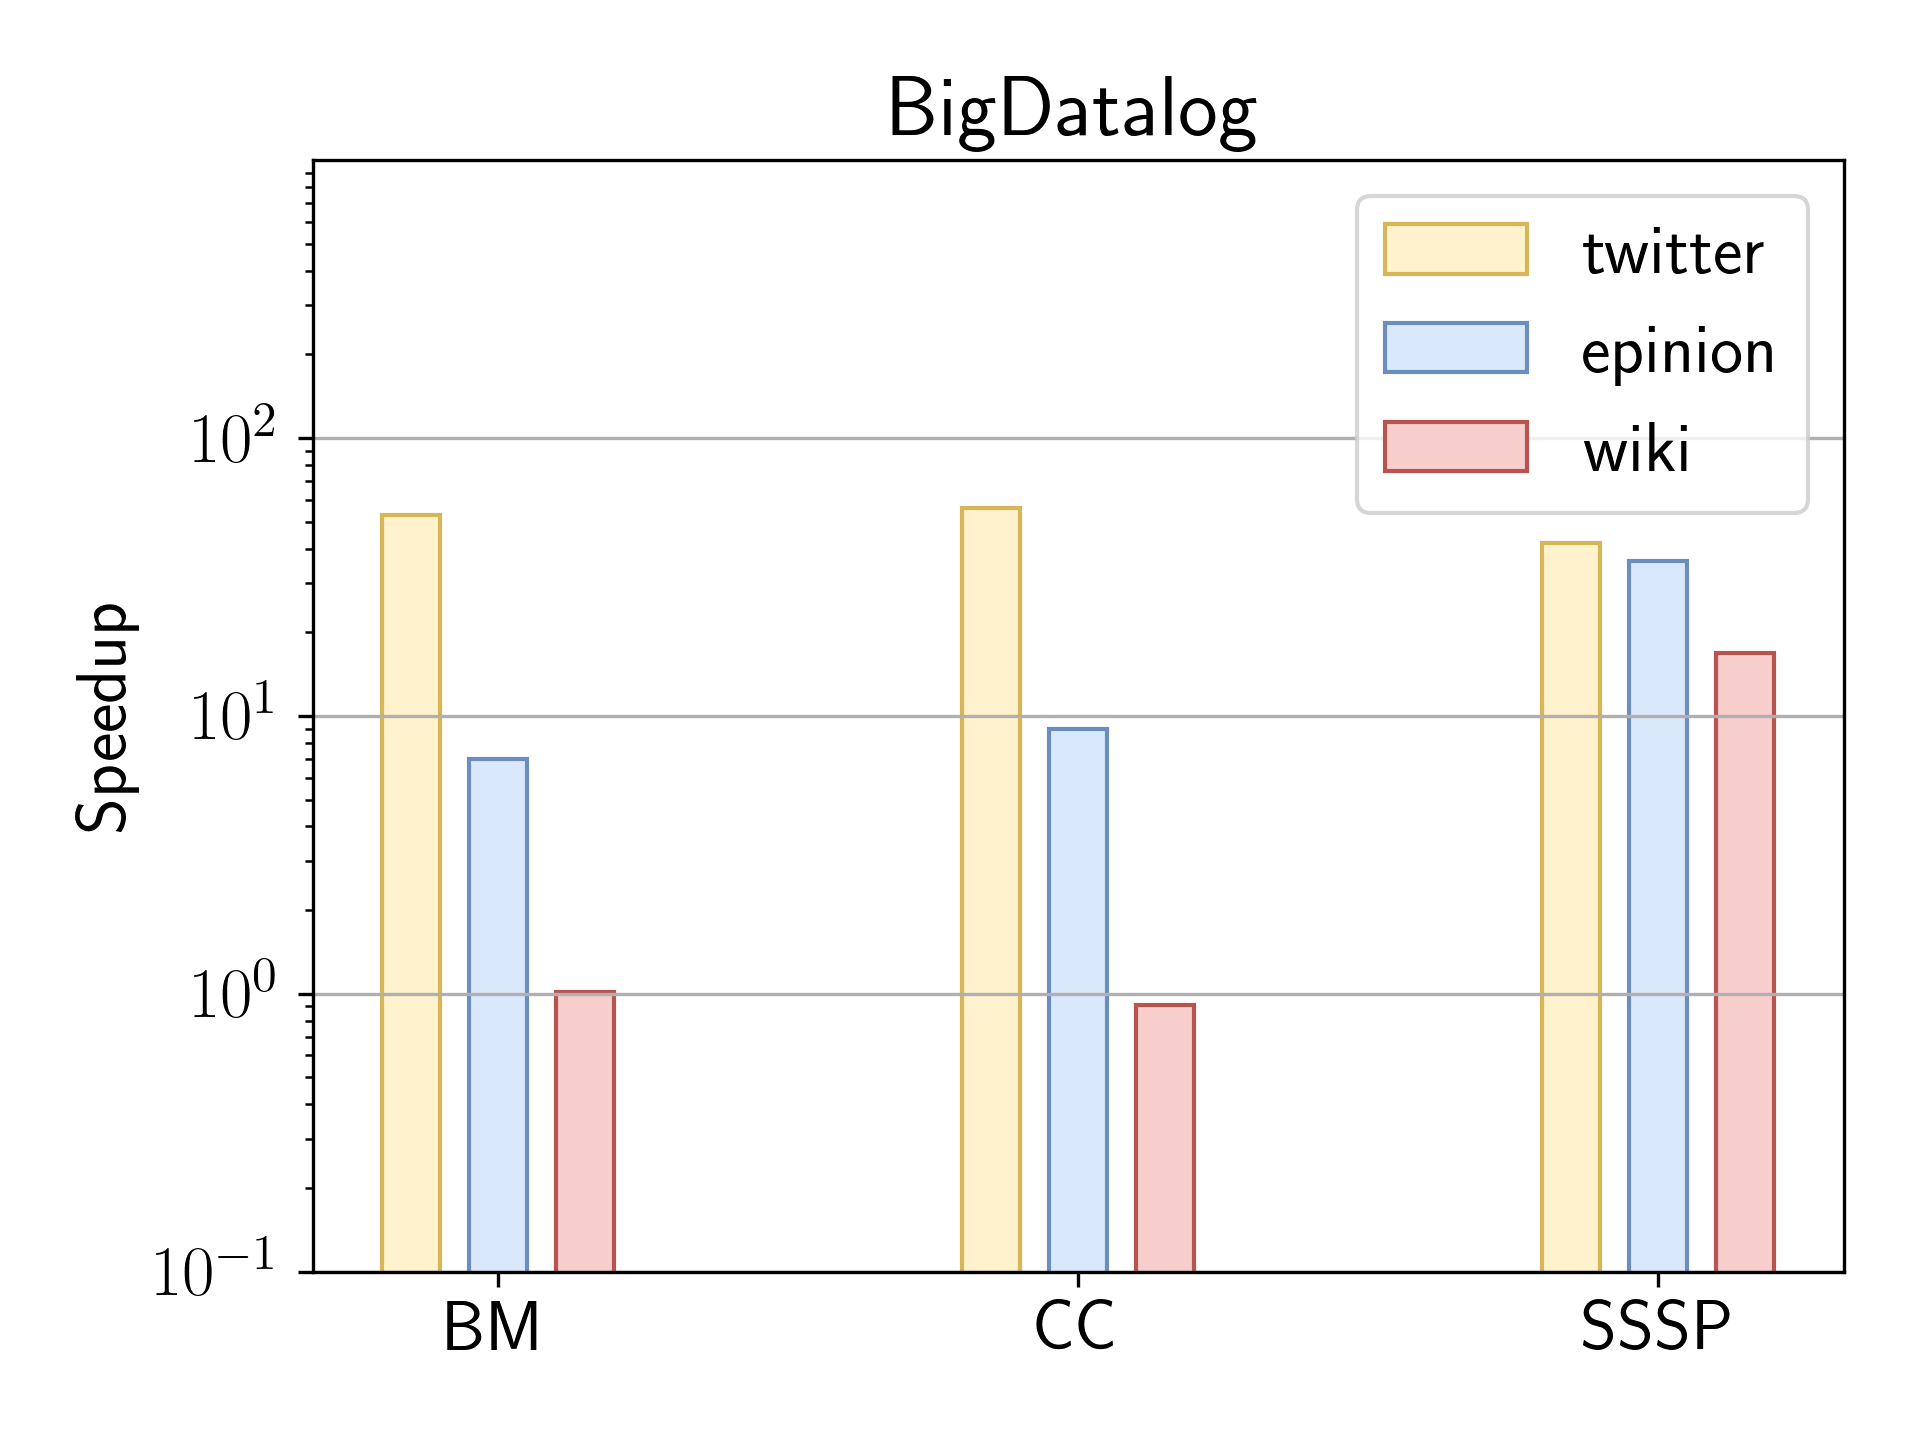
\includegraphics[width=\textwidth]{basic-bd}
        % \caption{BigDatalog}\label{fig:eval:basic:bd}
      \end{subfigure}

      \begin{subfigure}[b]{0.48\textwidth}
        \centering
        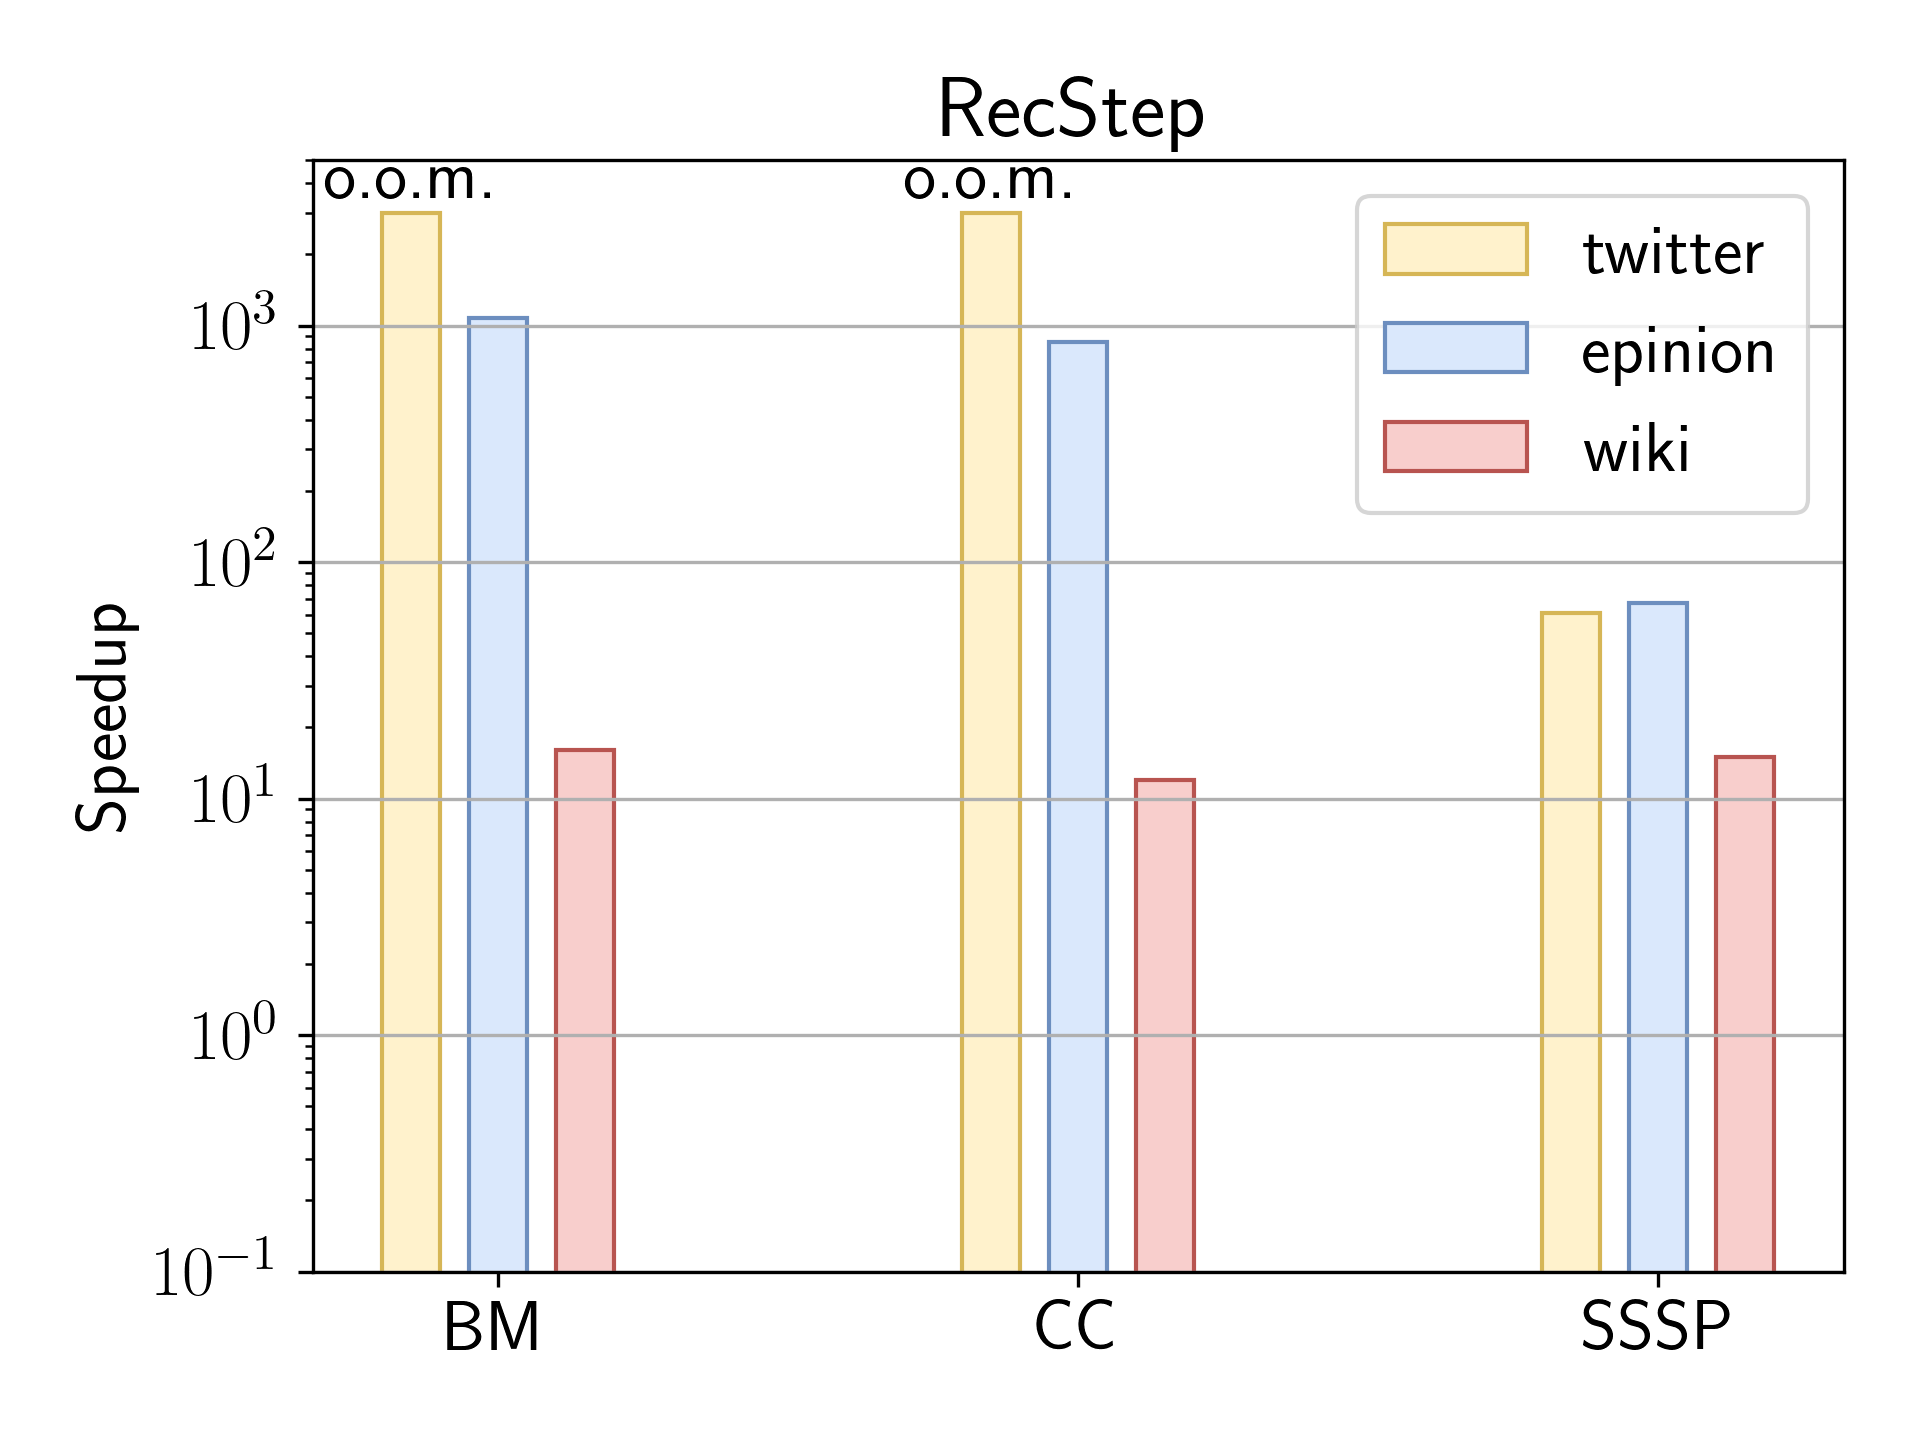
\includegraphics[width=\textwidth]{basic-rs}
        % \caption{RecStep}\label{fig:eval:basic:rs}
      \end{subfigure}
      \hfill
      \begin{subfigure}[b]{0.48\textwidth}
        \centering
        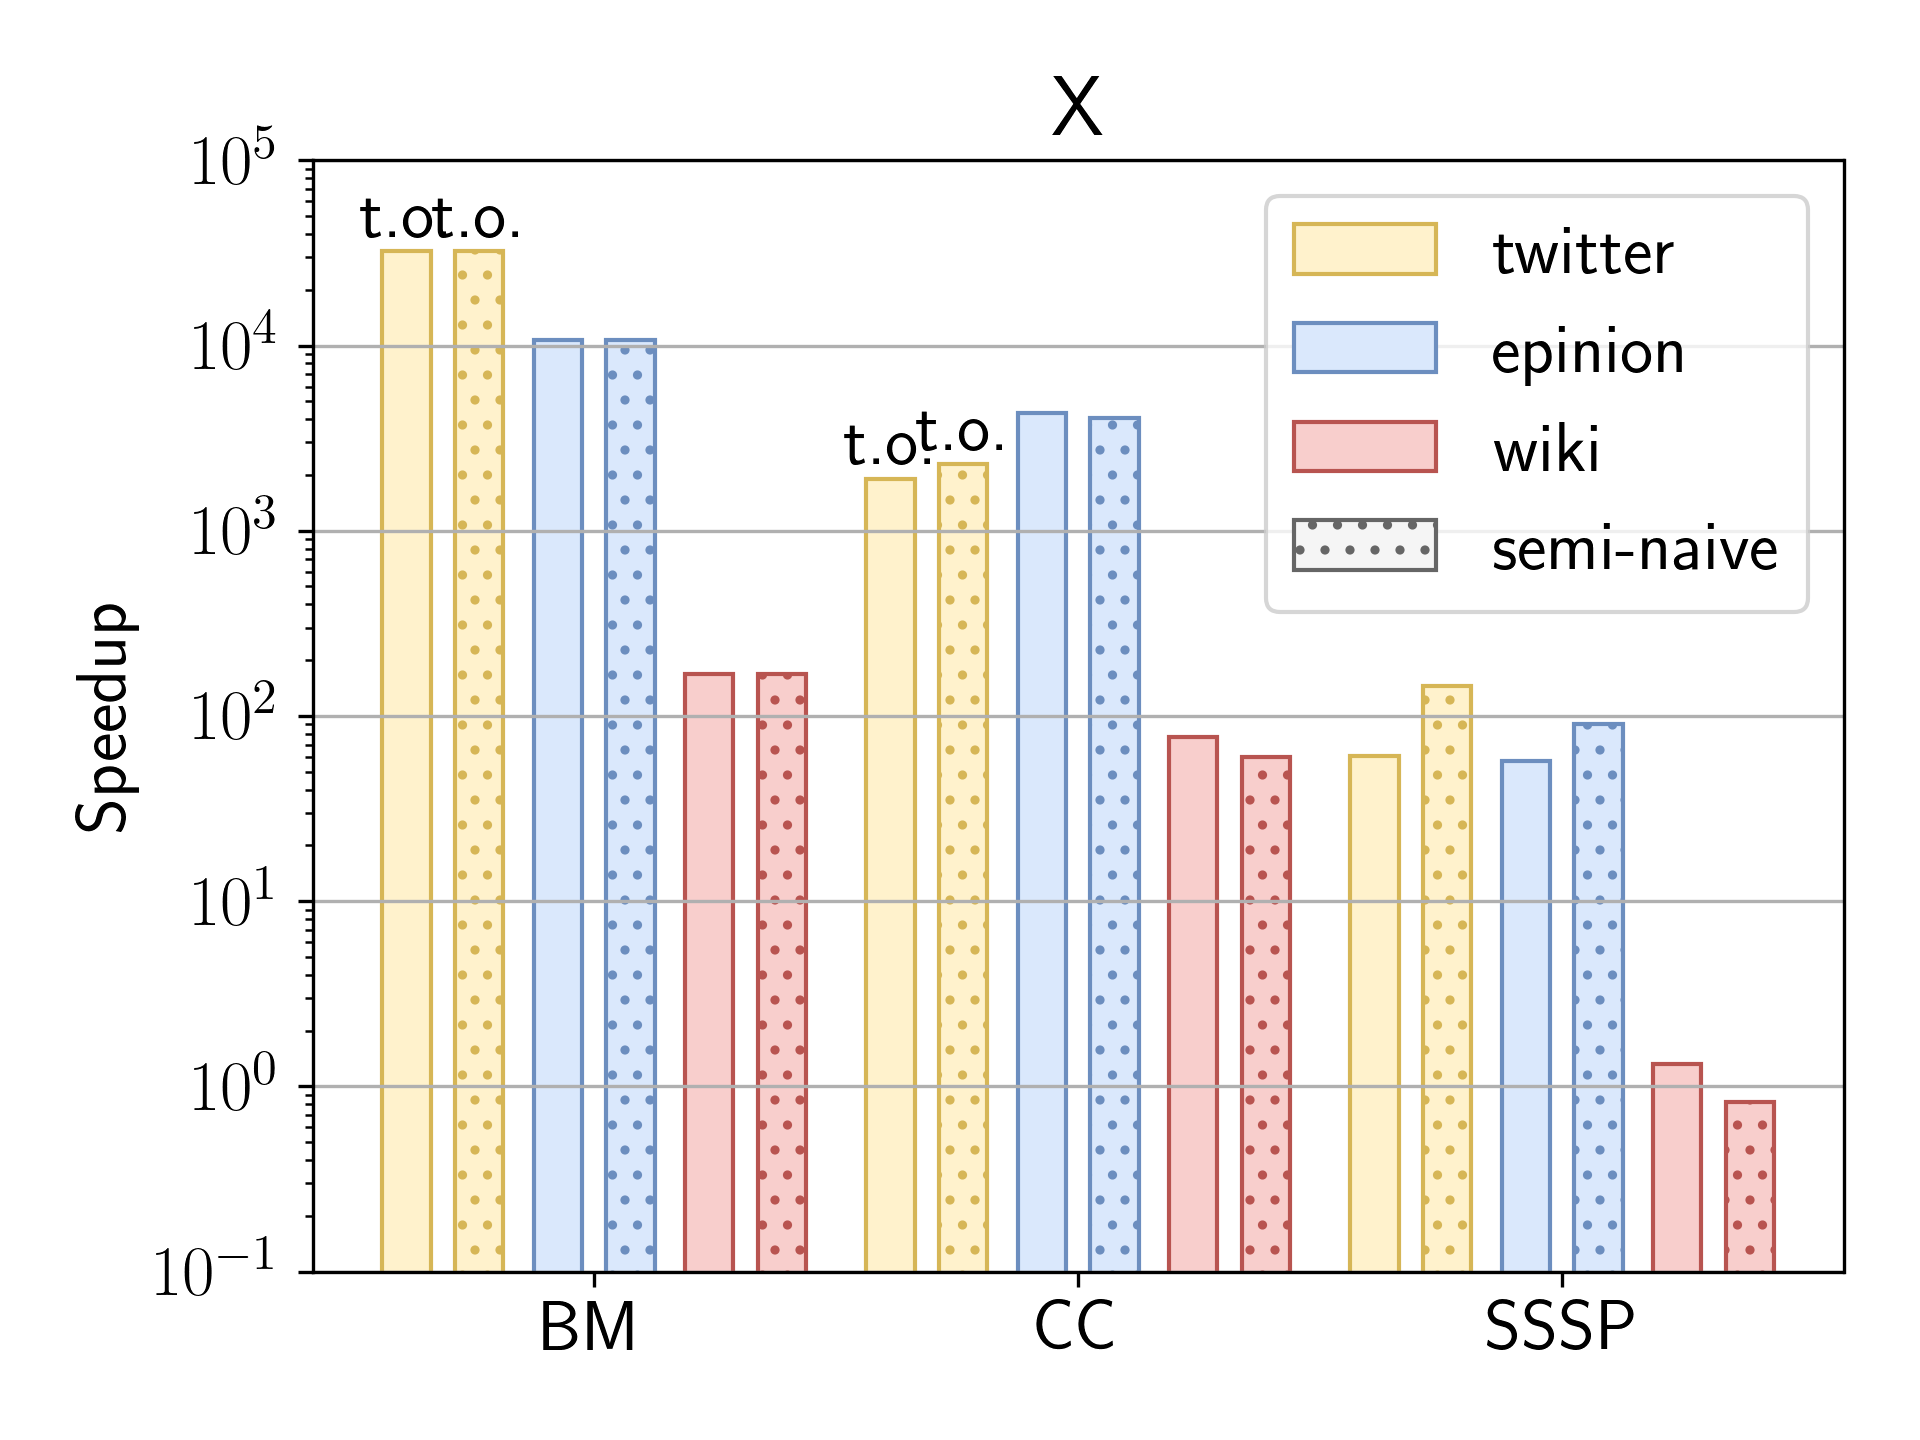
\includegraphics[width=\textwidth]{basic-x}
        % \caption{X}\label{fig:eval:basic:x}
      \end{subfigure}
      \caption{Speedup of the optimized v.s.\ original program; higher is better; 
      \required{t.o. means the original program timed out after 3 hours, in which case we report the speedup against 3 hours; o.o.m. means the original program ran out of memory.}}\label{fig:eval:eqsat}
    \end{figure*}
    
    \begin{figure*}
        \centering
        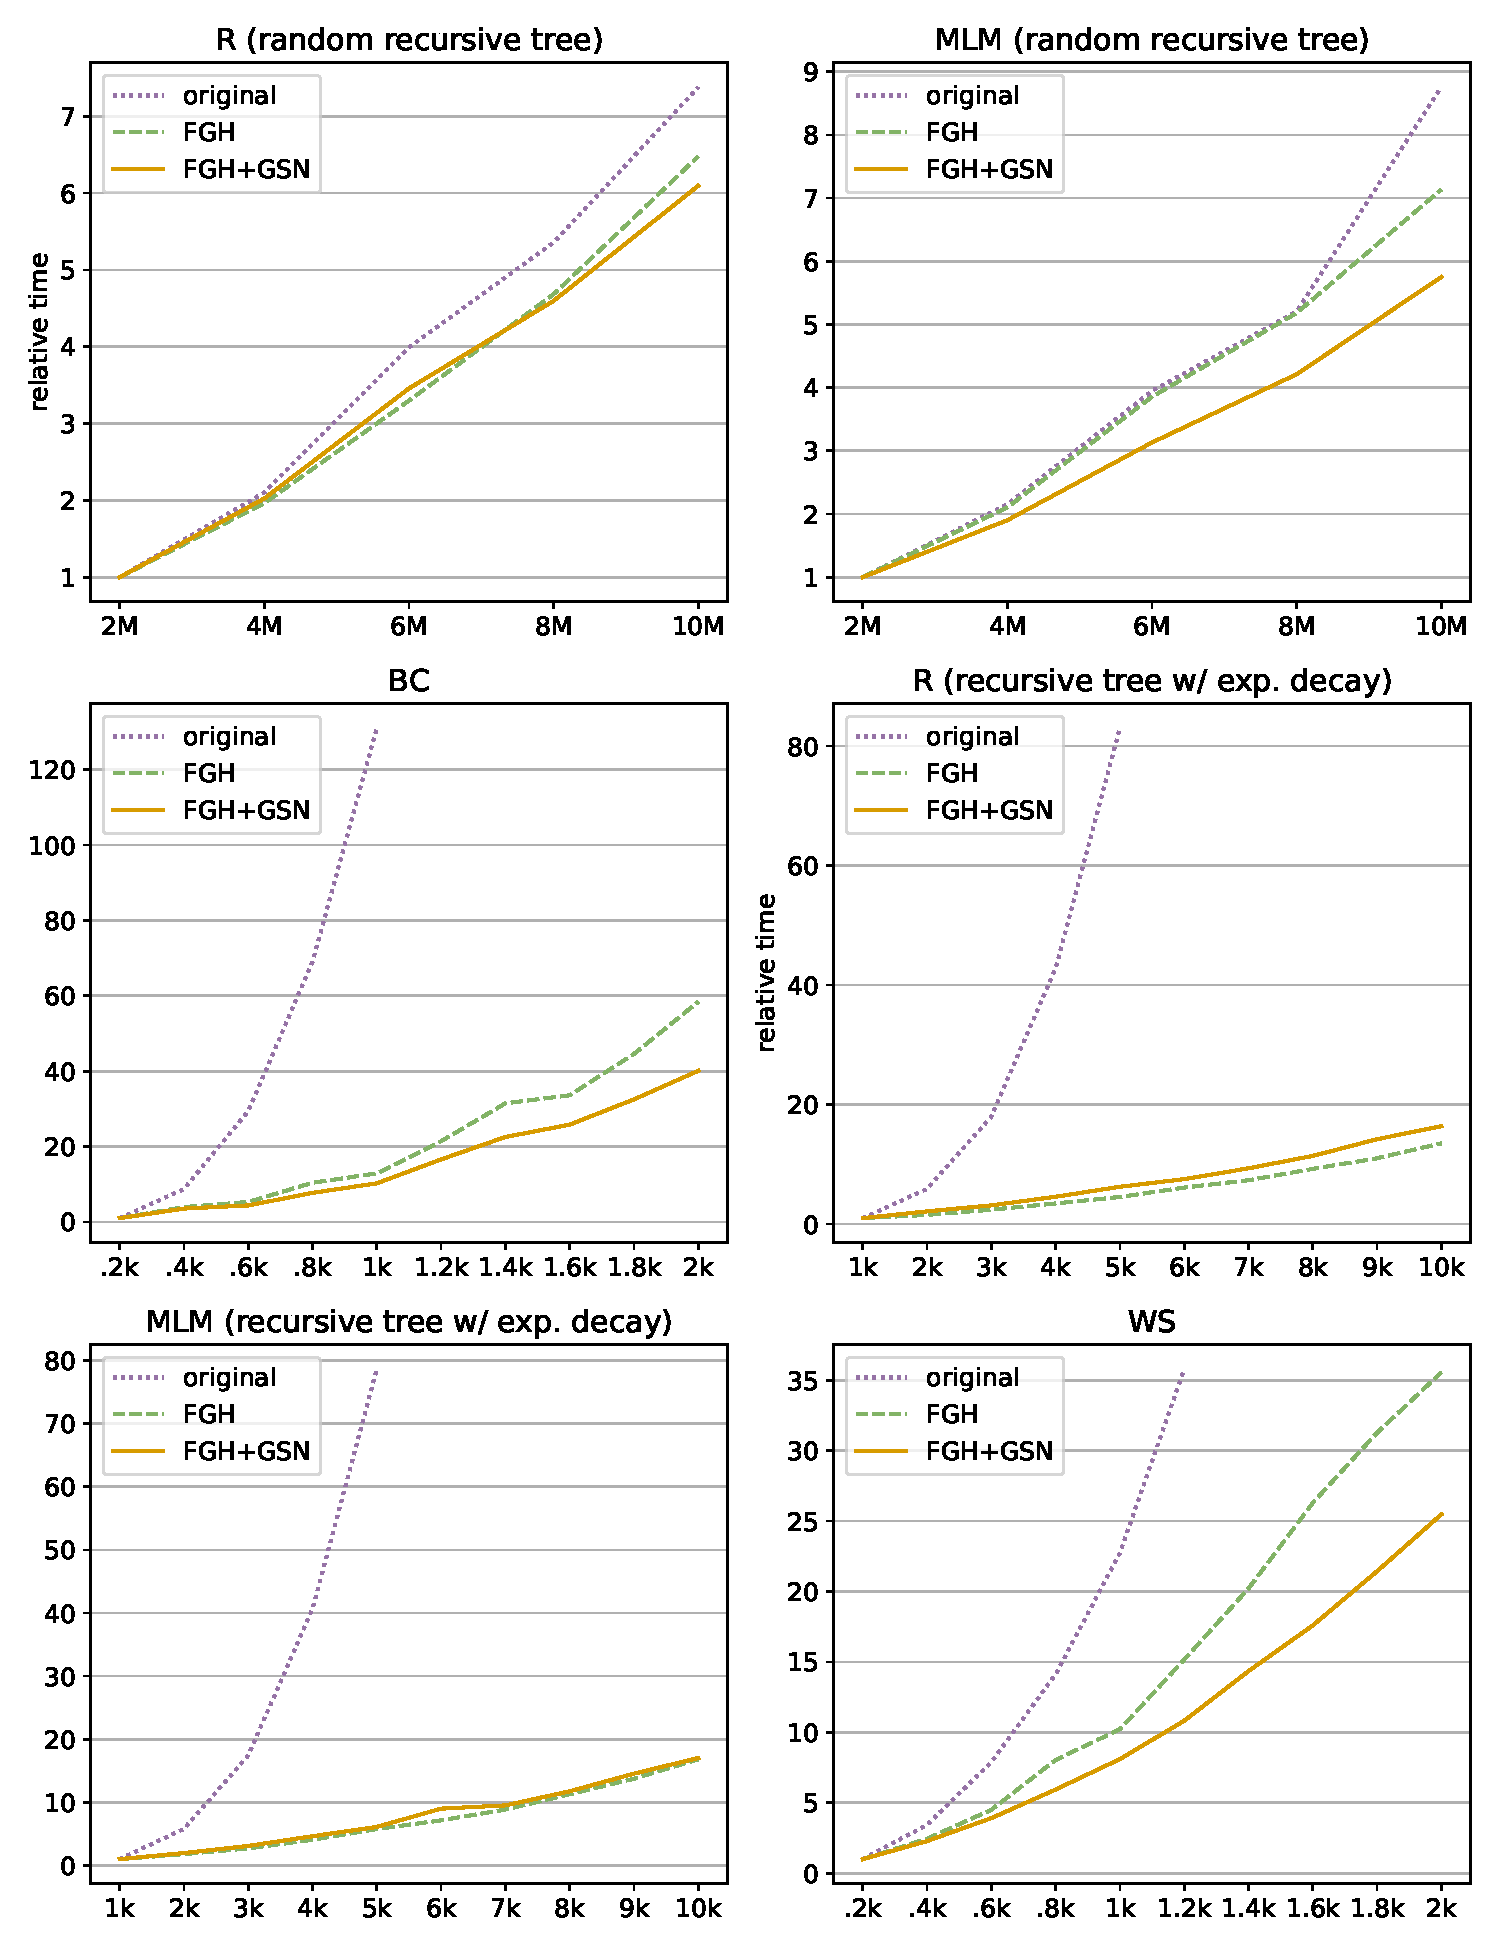
\includegraphics[width=\textwidth]{hard_bench}
        \caption{Runtime increase as a function of the data size; lower is  better.}\label{fig:eval:hard}
    \end{figure*}
    
    \begin{figure*}
      \centering
     \begin{tabular}{ c | c c c | c c c c }
     Program & BM & CC & SSSP & R & MLM & BC & WS \\
     \hline
     Invariance inference & 0.092 & 0 & 0 & 0.129 & 0.132 & 0 & 0\\
     Synthesis & 0.004 & 0.005 & 0.004 & 0.284 & 0.299 & 1.2 & 0.821 \\
     \hline
     Total & 0.096 & 0.005 & 0.004 & 0.413 & 0.431 & 1.2 & 0.821 \\
     Opt. / Exec. (max\%-min\%) & .82 - .16 & .04-.01 & .24-.002 & .41-.07 & .76-.09 & 6.3-.51 & 7.4-.66
    \end{tabular}

    \vspace{1em}

    \begin{tabular}{ c | c c c c }
     Program & R & MLM & BC & WS \\
     \hline
     Search space & 10 & 20 & 132 & 94 \\
    \end{tabular}
      \caption{Optimization time in seconds, 
      \required{optimization time over execution time,}
       and  size of the search space. }
      \label{fig:synthesis:time:space}
    \end{figure*}
    
    \section{Evaluation}\label{sec:eval}
    
    We implemented a source-to-source FGH-optimizer, based on
    Fig.~\ref{fig:arch}.  The input is a program $\Pi_1$, given by $F, G$,
    and a database constraint $\Gamma$, and the output is an optimized
    program $H$.  We evaluated it on three Datalog systems, and several
    programs from benchmarks proposed by prior
    research~\cite{BigDatalog, DBLP:journals/pvldb/FanZZAKP19}; we also
    propose new benchmarks that perform standard data analysis tasks.  We
    did not modify any of the three Datalog engines.  We asked two major
    questions:
    \begin{enumerate}
    \item How effective is our source-to-source optimization, given that
      each system already supports a range of optimizations?
    \item How much time does the actual FGH optimization take?
    \end{enumerate}
    
    \subsection{Setup}
    
    % \dan{Remy: we need 2-3 sentences explaining why you ended up with
    %   these systems, and examples of other systems that you considered but
    %   couldn't use}
    
    There is a great number of commercial and open-source Datalog engines in the
    wild, but only a few support aggregates in recursion.
    % Supporting non-recursive
    % aggregate is straightforward given any  Datalog engine: simply create a separate
    % stratum for the aggregation. Therefore, we only consider one system that lacks
    % recusive aggregate and use it as a baseline.
    We were able to identify five major systems with such support:
    SociaLite~\cite{DBLP:journals/tkde/SeoGL15},
    Myria~\cite{10.14778/2824032.2824052}, the DeALS family of systems
    (DeALS~\cite{DBLP:conf/icde/ShkapskyYZ15},
    BigDatalog~\cite{DBLP:conf/sigmod/ShkapskyYICCZ16}, and
    RaDlog~\cite{DBLP:conf/sigmod/0001WMSYDZ19}),
    RecStep~\cite{DBLP:journals/pvldb/FanZZAKP19}, and
    Dyna~\cite{francislandau-vieira-eisner-2020-wrla}.
    Prior work~\cite{BigDatalog} reports SociaLite and Myria are consistently slower than
    newer systems, so we do not include them in our experiments.
    Dyna is designed to experiment with novel language semantics and
    not for data analytics, and we were not able to run our benchmarks
    without errors using it.
    Systems in the DeALS family are similar to each other;
    we pick BigDatalog because it is open source
    and runs our benchmarks without errors;
    we include RecStep for the same reasons.
    Both BigDatalog and RecStep are multi-core systems.
    Finally, we run experiments on an unreleased commercial system X,
    which is single core.
    As we shall discuss, X is the only one that supports all features for
    our benchmarks.
    
    We conducted all experiments on a server running CentOS 8.3.2011.
    The server has a total of 1008GB memory, and
    4 Intel Xeon CPU E7-4890 v2 2.80GHz CPUs, 
    each with 15 cores and 30 threads. 
    We ran seven
    benchmarks, shown in Fig~\ref{fig:setup}. BM and CC are
    Examples~\ref{ex:more:magic} and ~\ref{ex:fgh:cc}; MLM is basically
    Example~\ref{ex:fgh:constraints}.  CC, SSSP and MLM are
    from~\cite{BigDatalog}, the others are designed by us.  R and MLM
    require a database constraint stating that the data is a tree.  BM,
    R, and MLM each have a non-trivial loop invariant that is inferred by the
    optimizer.  
    \required{Our optimizer requires each program to consist of two rules,
    one each for $F$ and $G$, and so a meaningful metric for
    program size is the number of semiring operations.
    These numbers are listed in the last column of Fig~\ref{fig:setup}.
    Our benchmark programs are comparable in size to those used in prior work~\cite{BigDatalog, DBLP:journals/pvldb/FanZZAKP19}.}
    All programs are available in our git repository.  The
    real-world datasets twitter~\cite{mcauley2012learning}, epinions~\cite{richardson2003trust}, and
    wiki~\cite{leskovec2010signed} are from the popular SNAP collection~\cite{snapnets}.  We
    follow the setting in~\cite{BigDatalog,DBLP:journals/pvldb/FanZZAKP19}
    when generating the synthetic graphs.
    We additionally generate random recursive trees with an exponential
    decay, modeling the decay of association in multi-level
    marketing~\cite{emek2011mechanisms}.
    For WS, we input the vector
    $[1, \ldots, n]$, since the values of the entries do not affect run time.
    In general, we used smaller datasets
    than~\cite{BigDatalog,DBLP:journals/pvldb/FanZZAKP19} because some of
    our experiments run single-threaded.
    
    
    
    
    
    \subsection{Run Time Measurement}
    
    %%% We measure the run time of Datalog programs drawn from benchmarks
    %%% proposed by prior research~\cite{BigDatalog, DBLP:journals/pvldb/FanZZAKP19};
    %%% we also propose new benchmarks that perform standard data analysis tasks.
    %%% We run the programs on real-world datasets drawn from popular
    %%% benchmarks as well as synthetic data.
    %%% The following table lists these programs and datasets:
    %%% 
    %%% The programs TC, CC, SSSP and MLM are drawn from~\cite{BigDatalog}.
    %%% We divide the programs into two groups in the table above:
    %%% the first group of 3 programs can each be optimized by the basic FGH-rule;
    %%% in other words, they require only rewriting (\eqsat) and not synthesis.
    %%% The second group of 4 require synthesis (\cegis);
    %%% programs R and MLM contain the integrity constraint
    %%% that the input is a tree.
    
    For each program-dataset pair, we measure the run times of three
    programs: original, with the FGH-optimization, and with the
    FGH-optimization and the generalized semi-naive (GSN, for short)
    transformation.  We report only the speedups relative to the original
    program in Fig.~\ref{fig:eval:eqsat} and~\ref{fig:eval:hard}.  In some
    cases the original program timed out our preset limit of 3 hours, 
    \required{where we report the speedup against the 3 hours mark.
    In some other cases the original program ran out of memory and we mark them with ``o.o.m.'' in the figure.
    }  The {\em absolute} runtimes are irrelevant
    for our discussion, since we want to report the effect of {\em adding}
    our optimizations.  (We also do not have permission to report the
    runtimes of X.)  All three systems already perform semi-naive
    evaluation on the original program, since that is expressed over the
    Boolean semiring.  But the FGH-optimized program is over a different
    semiring (except for BM), and GSN has non-stratifiable rules with
    negation, which are supported only by system X; we report GSN only for
    system X.  While the benchmarks in Fig.~\ref{fig:eval:eqsat} were on
    real datasets, those in Fig.~\ref{fig:eval:hard} use synthetic data,
    for multiple reasons: we did not have access to a good tree dataset
    needed in the R and MLM benchmarks, BC timed out on our real data (BC
    is computationally expensive), and WS uses only a simple array.  A
    benefit of synthetic data is that we can report how the optimizations
    scale with the data size.  Unfortunately, the FGH-optimized programs
    in Fig.~\ref{fig:eval:hard} require recursion with \textsf{SUM}
    aggregation, which is not supported by BigDatalog or RecStep; this is
    in contrast with those in Fig.~\ref{fig:eval:eqsat}, which require
    recursion with \textsf{MIN} aggregation which is supported by all
    systems.
    
    % before and after optimization; when applicable, we also measure the
    % speedup with and without generalized semi-naive transformation (GSN,
    % for short).  Note that expressing GSN requires non-monotone rules and
    % non-stratifiable negation.  At the time of writing only X supports
    % both of these features.  BigDatalog and RecStep also do not support
    % recursive \textsf{SUM}, which is necessary for the FGH-optimized
    % programs BC and MLM.  For these reasons we run the second group of
    % benchmarks on X only.  We cannot report the raw run time of X, and
    % since the experiments are not meant to compare the systems against
    % each other, we only report speedup and relative time.
    
    
    \subsubsection{Findings} Figure~\ref{fig:eval:eqsat} shows the results
    of the first group of benchmarks optimized by the
    rule-based synthesizer.  Overall, we observe our optimizer provides
    consistent and significant (up to 4 orders of magnitude) speedup across
    systems and datasets.  Only a few datapoints indicate the optimization
    has little effect: BM and CC on wiki under BigDatalog, and SSSP on
    wiki under X.  This is due to the small size of the wiki dataset: both
    the optimized and unoptimized programs finish very quickly, so the run
    time is dominated by system overhead which cannot be optimized away.
    We also note that (under X) GSN speeds up SSSP but slows down CC (note the log scale).
    The latter occurs because the $\Delta$-relations for CC are very large,
    and as a result the semi-naive evaluation has the same complexity as
    the naive evaluation; but the semi-naive program is more complex and
    incurs a constant slowdown.  GSN has no effect on BM because the
    program is in the boolean semiring, and X already implements the
    standard semi-naive evaluation.
    Optimizing BM with FGH on BigDatalog sees a significant speedup even though the
    systems already implements magic set rewrite,
    because the optimization depends on a loop invariant.\footnote{
    BigDatalog can optimize the left-recursive version of BM~\eqref{eq:simple:magic:nonopt}
    to obtain similar speedup, via the classic magic set rewrite.}
    Overall, both the semi-naive and
    naive versions of the optimized program are significantly faster than
    the unoptimized program.
    
    Figure~\ref{fig:eval:hard} shows the results of the second group of
    benchmarks, which required \cegis.  Since we used synthetic data,  we
    examined here the asymptotic behavior of the optimization as a
    function of the data size.
    % The programs in this group are
    % more complex and take longer to run, so we limit our data size to
    % ensure the experiments finish in reasonable time.  
    The most advanced optimization was for BC, which leads essentially to
    Brandes' algorithm~\cite{brandes2001faster}: its effect is dramatic.
    R and MLM rely on semantic optimization for a tree.  We generated two
    synthetic trees, a random recursive tree with expected depth of
    $O(\log n)$ and one with exponential decay with expected depth of
    $O(n)$.  Since the benefit of the optimization depends on the depth,
    we see a much better asymptotic behavior in the second case.  Here,
    too, the optimizations were always improving the runtime.
    
    % 
    % 
    % Overall, we observe weak asymptotic speedup for R and MLM on random
    % recursive trees, and strong asymptotic speedup in all other cases.
    % Recall programs R and MLM constrain their input to be trees.  For the
    % two programs, the optimized programs are only slightly faster than the
    % unoptimized one.  Closer examination of the optimized code reveals
    % similar complexity as the unoptimized one.  For example, the original
    % MLM first computes the transitive closure of size $O(n\log(n))$ where
    % $n$ is the size of the tree.  This only leaves a $\log(n)$ factor to
    % be optimized away, so the optimized programs are not much faster
    % despite requiring only linear space.  The speedup becomes much more
    % pronounced when we introduce exponential decay when generating the
    % random trees.  Then the trees are much deeper (with $\Omega(n)$
    % depth), which forces the transitive closure in the unoptimized program
    % to take space $\Omega(n^2)$, whereas the optimized programs still run
    % in linear space.
    % % Notably, the programs run slightly slower under semi-naive evaluation. 
    % % This is also caused by the large depth of the tree:
    % % the higher nodes are shared by many paths to the root, 
    % % and will be repeatedly updated with new deltas throughout semi-naive
    % % evaluation. 
    % For BC and WS, the naive version of
    % the optimized program already speeds up the program significantly, and
    % the semi-naive version contributes further speedup.  
    % 
    
    % \reinhard{Is it clear what SN and OG in  Figure~\ref{fig:eval:hard}  mean? Should SN be replaced by GSN? What about OG?}
    
    \subsection{Optimization Time and  Search Space}
    
    \cegis\ can quickly become very expensive if its search space is
    large, and, for that reason, we have designed the grammar generator
    carefully to reduce the search space without losing generality.
    Fig.~\ref{fig:synthesis:time:space} reports the runtime of the
    synthesizer (in seconds) for both rule-based synthesis and \cegis, and the size
    of the search space.  The rule-based synthesizer runs in
    milliseconds, while \cegis\ took over 1s for BC (our hardest
    benchmark).  These numbers are close to those demanded by modern query
    optimizers, and represent only a tiny portion of the total runtime
    of the optimized query. 
    \required{
    Optimization time takes less than 1\% of the query run time for all benchmarks except for BC and WS on the smallest input data. }
    To our surprise, our grammar managed to
    narrow the search space considerably, to no more than 132 candidates,
    which (in hindsight) explains the low optimization times. 
    \required{
    The search space can grow rapidly, and even exponentially, 
    as the size of the input program grows.
    Our optimizer optimizes a single stratum at a time, 
    focusing on improving critical ``basic blocks'' of a program.
    Our benchmark programs demonstrate a wide range of data analysis computation can
    be expressed succinctly using just a few semiring operations, 
    and optimization can have a dramatic impact on performance.}
    
    \subsection{Summary}
    
    We conclude that our optimizer can significantly speedup already
    optimized  Datalog  systems, either single-core or multi-core.  GSN
    can, sometimes, further improve the runtime.  We achieved this using a
    rather small search space, which led to fast optimization.
    
    
    % programs across different execution engines and datasets.  In some
    % cases, GSN is necessary to achieve the best performance; in other
    % cases GSN has no effect or even slightly slows down the optimized
    % program.  Since the GSN transformed programs are almost always faster
    % than the baseline, we argue it should be implemented in future Datalog
    % systems.
    % 
    % \reinhard{Wouldn't it be nicer if we could conclude by emphasizing the benefit of {\em our} optimization 
    % rather than of GSN (or at least mention that the combination of the two is unbeatable)?}
    
    % \subsection{Compilation Time}
    % Figure~\ref{fig:synthesis:time:space} shows the compile time breakdown
    % for each program.
    % %
    % \reinhard{Should we state that the numbers in the table are to be understood as 
    % ``percent relative to the run time of the unoptimized program''?}
    % %
    % Overall, compilation takes under $1\%$ of the total
    % run time of the unoptimized program.
    % All programs from the first group are compiled faster than those from the
    % second.
    % This is because optimizing the first group does not require synthesis
    % and only involves \eqsat, which is very fast.
    % In our implementation we invoke invariant inference on demand.
    % That is, we first attempt optimization without invariants,
    % and only when this fails do we invoke invariant inference.
    % Since optimizing CC, SSSP, BC and WS does not require invariants,
    % we skip the inference step.
    % 
    
    
    %%% Local Variables:
    %%% mode: latex
    %%% TeX-master: "main"
    %%% End:

    % \section{Summary and Discussion}
\chapter{Conclusions}
\label{chap:conclusions}

\clearpage
\addcontentsline{toc}{chapter}{Bibliography}
\singlespacing
\bibliographystyle{alpha}
\bibliography{references}

\end{document}
